\section{Study Results}
\label{study_results}
We answer two research questions by analyzing of our survey responses and by comparing our results against surveys conducted for other countries:
\begin{enumerate}[label=RQ\arabic{*}., leftmargin=26pt]
  \item What are the software development practices in an emerging country like Bangladesh? (Section \ref{RQ1})
  \item How do the development practices in Bangladesh differ from other developed countries? (Section \ref{RQ2})
\end{enumerate}
% \section{Study Results}
% \subsection{Development Practices and Processes in Bangladesh (RQ1)}
% We divide this into four sub-questions:
% \begin{enumerate}
%     \item What software methodology are used in your project?
%     \item Which implementation technologies and tools are adopted by software
% development professionals?
% \item  What type of testing and deployment practices are used?
% \item How are the security and performance is ensured in a product of a company?
% \end{enumerate}
% \subsection{Comparison among countries (RQ2)}
% We do the comparison along the following dimensions:
% \begin{enumerate}
%     \item Development methods and practices
%     \item Implementation technologies
%     \item Quality assurance
%     \item Release and iterations
% \end{enumerate}

%We have explored two research questions in this study. 
The first research question focuses on the dimensions of software development
practices and processes in Bangladesh. The second research question compares those
practices prevailing in Bangladesh with other regions to reveal the similarities
and dissimilarities in software development practices and processes.

\subsection{Development Practices and Processes in Bangladesh (RQ1)}
\label{RQ1}
Following previous studies in region-based software development process analysis~\citep{Garousi2013, Garousi2015, Vonken2012, Wang2018}, we 
analyze the development practices and processes in Bangladesh along four dimensions (D):
\begin{enumerate}[label=D\arabic{*}., leftmargin=20pt]
  \item Software development methodologies used (Section \ref{methodology}). We investigate the development
processes, methodologies, requirements analysis processes.
  \item Software tools and techniques used (Section \ref{tools}). We determine the
trending technologies like platforms, programming languages, and frameworks.
\item Software testing and devops practices used (Section \ref{testing_practices}). We explore the
present situation of testing and deployment practices.
\item Performance and security measures used (Section \ref{security_performance}). We analyze how
software companies secure and maintain their code and what practices are
followed to ensure performance and scalability.
\end{enumerate}
%We divide this into the following four sub-questions which explore software development practices and processes in Bangladesh in more detail.

\subsubsection{What software methodology are used in your project?}
\label{methodology}

Software development methodology implies the process used for developing particular information systems in a very deliberate, structured, and methodical way. Through this question, we address the fundamental component of development practice in a company. We report the following relevant results:

\begin{itemize}
\item Software development methodologies (Q 6).
\item Requirements gathering (Q 7).
\item Most time-consuming software development activities (Q 8).
\end{itemize}


\paragraph{Software development methodologies}
In our study, as per Figure \ref{fig:methodologies}, we have found that the most popular software development model in Bangladesh is Agile with a response rate of 64\%. The next widely-used model among our respondents is Scrum with a response rate of 46\%. These outcomes match the 2018 Stack Overflow (SO) survey \cite{StackoverflowSurvey2018} result, which reports that Agile and Scrum are the most popular methodologies for developers worldwide keep their projects on track. However, the other methodologies have lower usage rates based on our survey participants: pair programming (20\%), Waterfall (12\%), etc.


\paragraph{Requirements gathering}
The most critical activity that always arises during software development is collecting and analyzing the requirements of a system. Usually, the outcome of the analysis is presented before the client and modified according to their feedback. The more clear and detailed requirements are, the higher the possibility of building software that conducts the client’s anticipation. Corresponding to Figure \ref{fig:requirements}, using plain text (44\%) and storyboard (41\%) are the most widely used requirement gathering techniques among our survey participants. The other relevant techniques include use case (36\%), GUI prototype (35\%), grooming session (30\%), etc. Here we see an appreciable percentage of software practitioners prefer plain text to collect requirements rather than using standard techniques. This is an important finding that requires further analysis for causes and to analyze the potential effects of not practicing standard requirements gathering techniques frequently. \anindya{The rationality of the last line is not clear.} \khalid{updated}

\begin{figure}[h]
\centering
  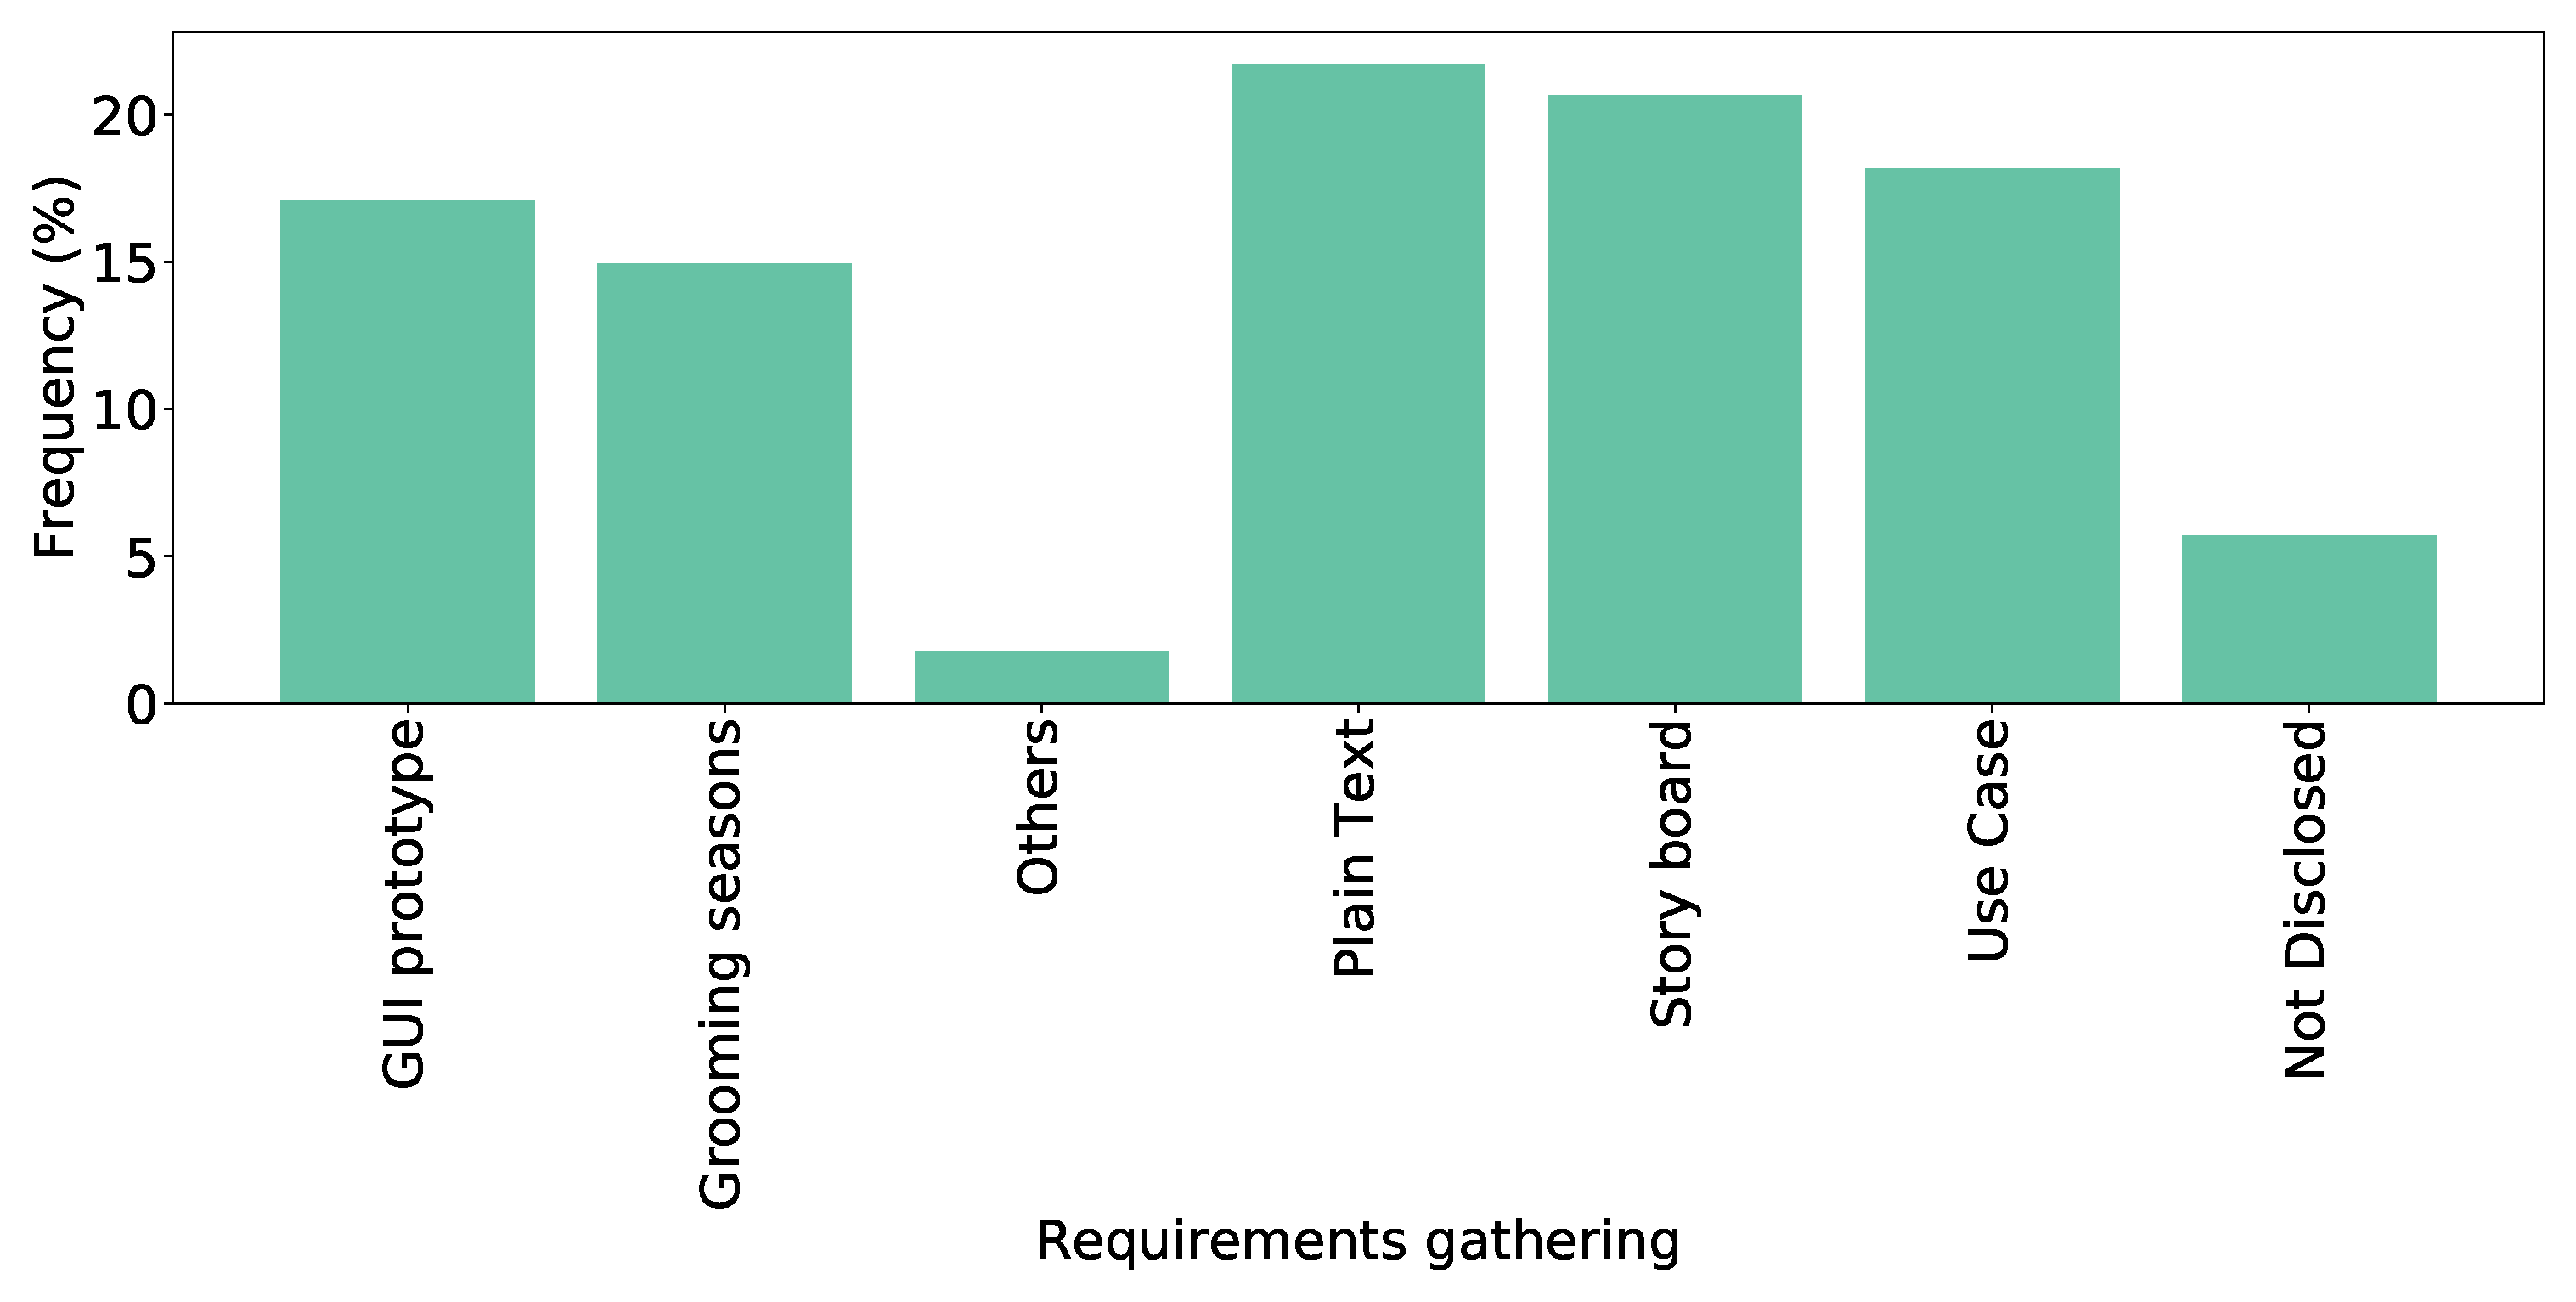
\includegraphics[scale=0.18]{Figures/Requirements_Gathering}
  \caption{Requirements gathering}
  \label{fig:requirements}
\end{figure}


\paragraph{Timeline of Development Activities}
Here, the participants were asked about the most time-consuming software development activities as far as their experience goes. We have presented the activities with respect to the percentage of the participants in Figure \ref{fig:activities}. We see that, according to 65\% of our respondents, most of the time is spent in the implementation stage, whereas the requirement analysis stage requires the second most according to 45\% response. The other usages are program design (37\%), project planning (30\%), testing (19\%), maintenance (17\%), etc.

\begin{figure}[h]
\centering
  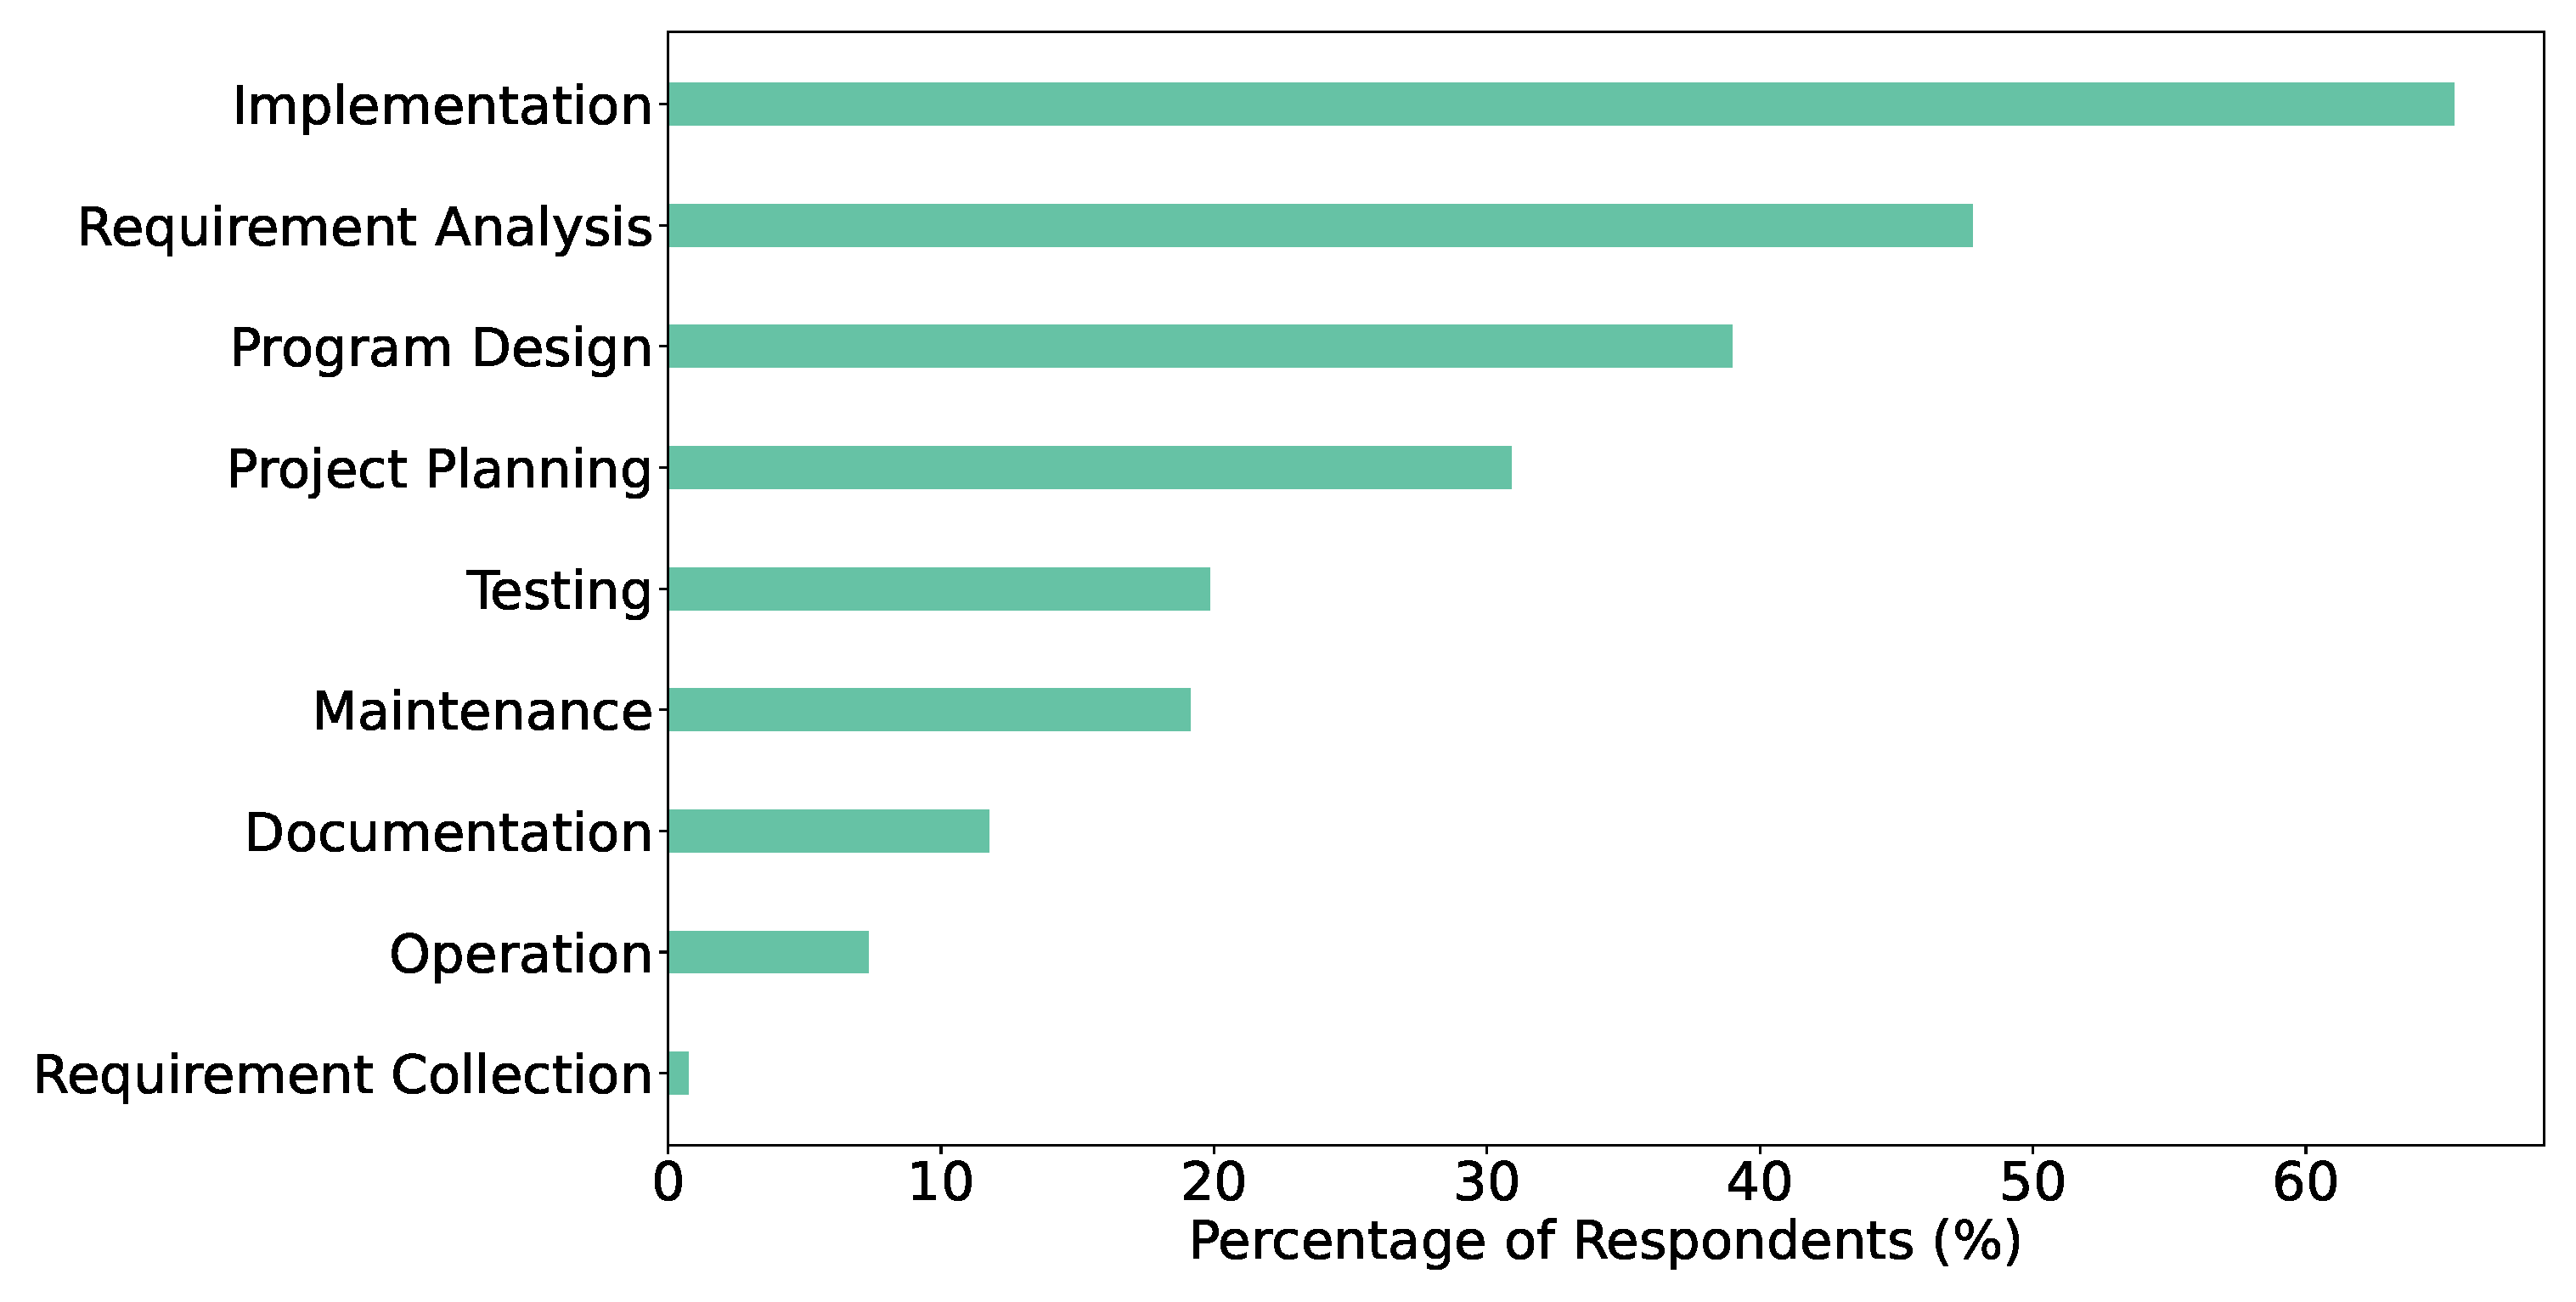
\includegraphics[scale=0.2]{Figures/Respondents_Activities}
  \caption{Software development activities}
  \label{fig:activities}
\end{figure}

We expected that there would be some correlation between software development methodologies (Q6) and the most time-consuming development activities (Q8). Some methodology may add extra time in development activities. \anindya{The previous line does not make clear sense. Can it be rephrased?}\partha{updated}. Thus we have calculated the Cramér`s V \cite{Cramer1946} between the choice of software development methodologies and most time spent activity of the respondents. Cramér`s V calculates the measure of association between two nominal variables\cite{Sheskin2007}. However, we have not found any significant correlation.

\begin{figure}[h]
\centering
  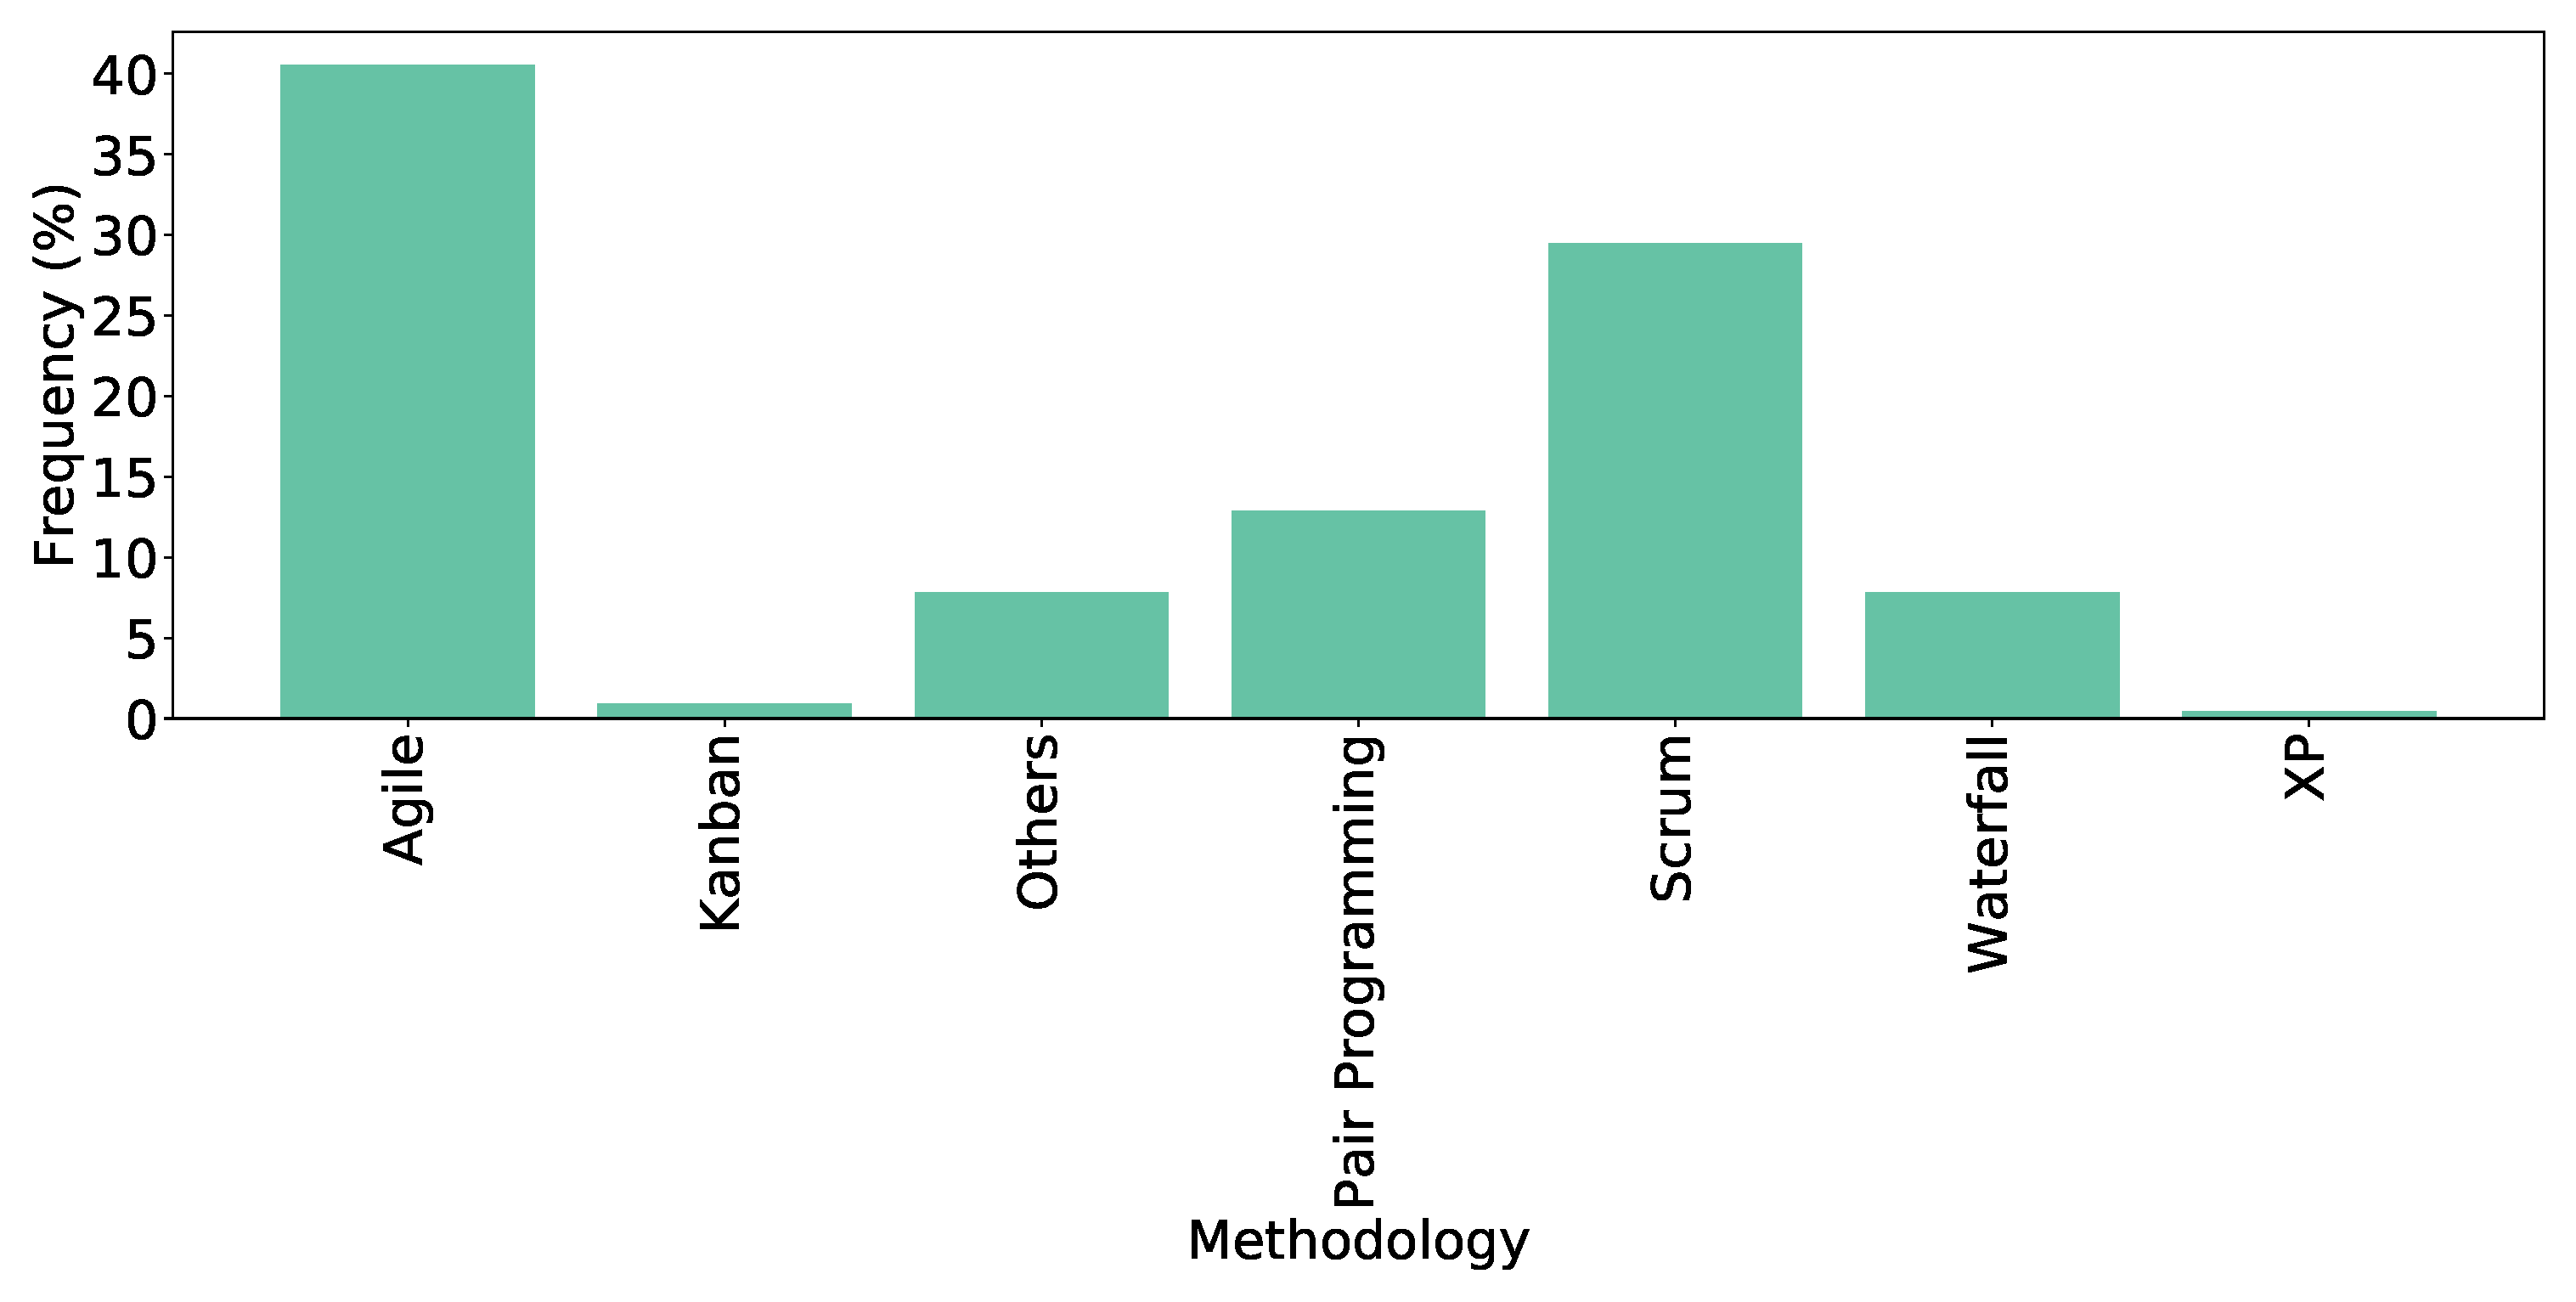
\includegraphics[scale=0.18]{Figures/Respondents_Methodology}
  \caption{Software development methodologies}
  \label{fig:methodologies}
\end{figure}

We guessed that there might be a relation between developers' experience and their activities. It is a general idea that senior developers spend most of their time in requirement specification and design activities, where junior developers spend their time implementing the solution. For analysis purposes, we divided our respondents into two groups based on their professional experience. The two groups are 1) Senior: Developers with more than 5 years of experience 2) Junior: Developers having less than 5 years of experience. We plotted the most time spent activity for the above-mentioned two groups in Figure \ref{fig:activity and seniority}. \anindya{This line is not clear.}\partha{updated}. We can see that our anticipation is right. Junior developers are mostly engaged in the implementation, where senior developers are engaged with requirement specifications.
\anindya{Do you consistently imply coding/development by implementation? In SE, it has a different meaning.}\partha{`Implementation' was one of the options of this closed question. It seems like respondents used it to mean coding/development. One of the responses to another question was `Implementation time carefulness and maintaining a well-developed coding standard.' Though I am not sure, it seems he means coding/development here}

\begin{figure}[h]
\centering
  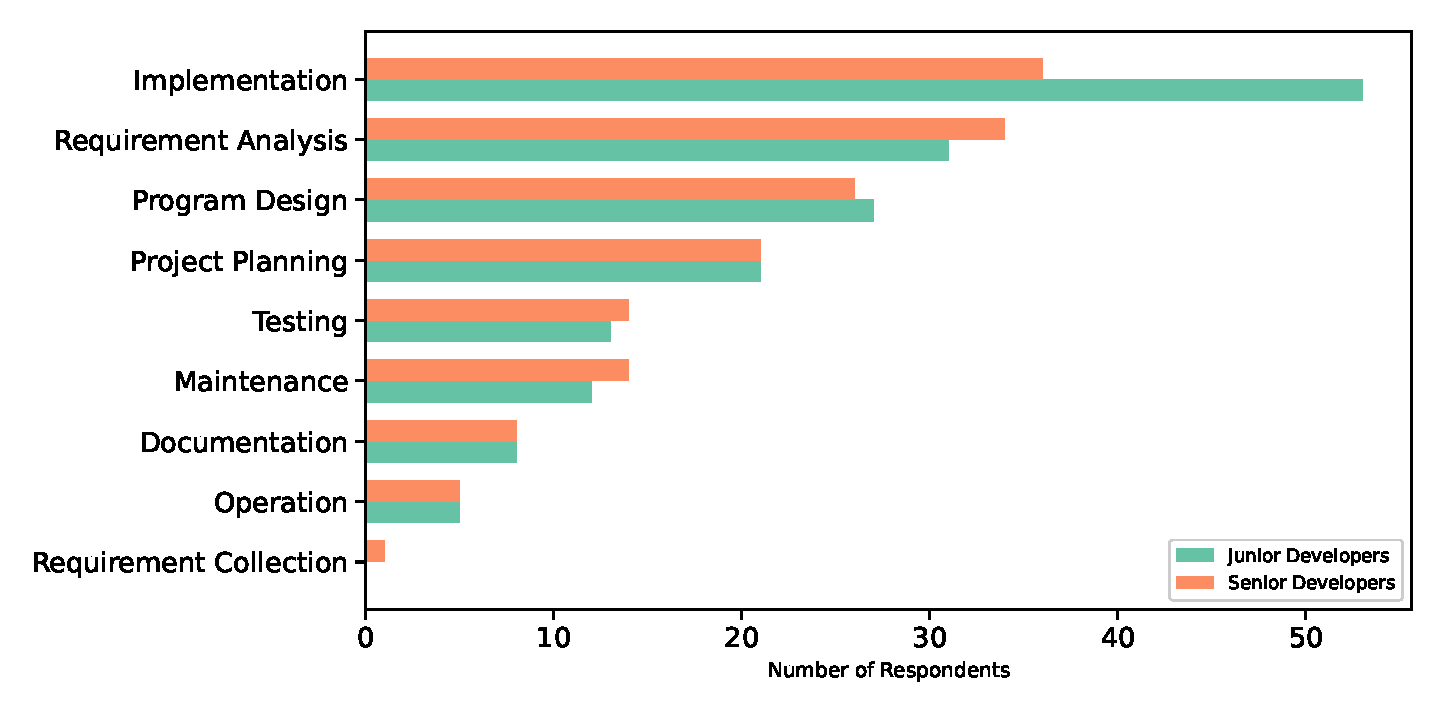
\includegraphics[scale=0.4]{Figures/Activity_and_Seniority.eps}
  \caption{Relation between seniority and activity}
  \label{fig:activity and seniority}
\end{figure}
\partha{In the survey the activity was a multiple choice field. Not sure we can perform any stat. analysis. Will it be theoretically correct?}

\boxtext{Developers of the Bangladeshi SE industry generally spend more time on implementation-related activities than planning and testing.}

\subsubsection{Software development tools and techniques used (D2)}
\label{tools}
%\anindya{Implementation or development??}
We ask five questions related to technologies and tools that are
adopted by software development professionals: \begin{inparaenum}
\item Technology Platform (Q9).
\item Operating System (Q10).
\item Programming Language (Q11).
\item Framework (Q12).
\item IDE (Q13).
\end{inparaenum}

For technology platforms (Q9), most of our survey respondents (80\%) work for the web
platform (Figure \ref{fig:platforms}). The rests are mobile (45\%), desktop (30\%), embedded/IoT
(8\%). This distribution is similar to the 2020 wordwide survey of JetBrains \cite{JetBrains2020}, which finds that 
websites are the
most common type of application developers work on, and the web platform is the
most preferable and popular to develop, followed by desktop and mobile. We have conducted a cross-aspect analysis to identify any relationship
between the technology platform and the requirement gathering process. The
bubble charts in Figure \ref{fig:requirement technology cross analysis}
visualize the cross-aspect analysis. It is clear from the figure that the
requirement gathering process is mostly practiced in GUI-based development
(e.g., web, desktop, mobile).
\begin{figure}[t]
\centering
  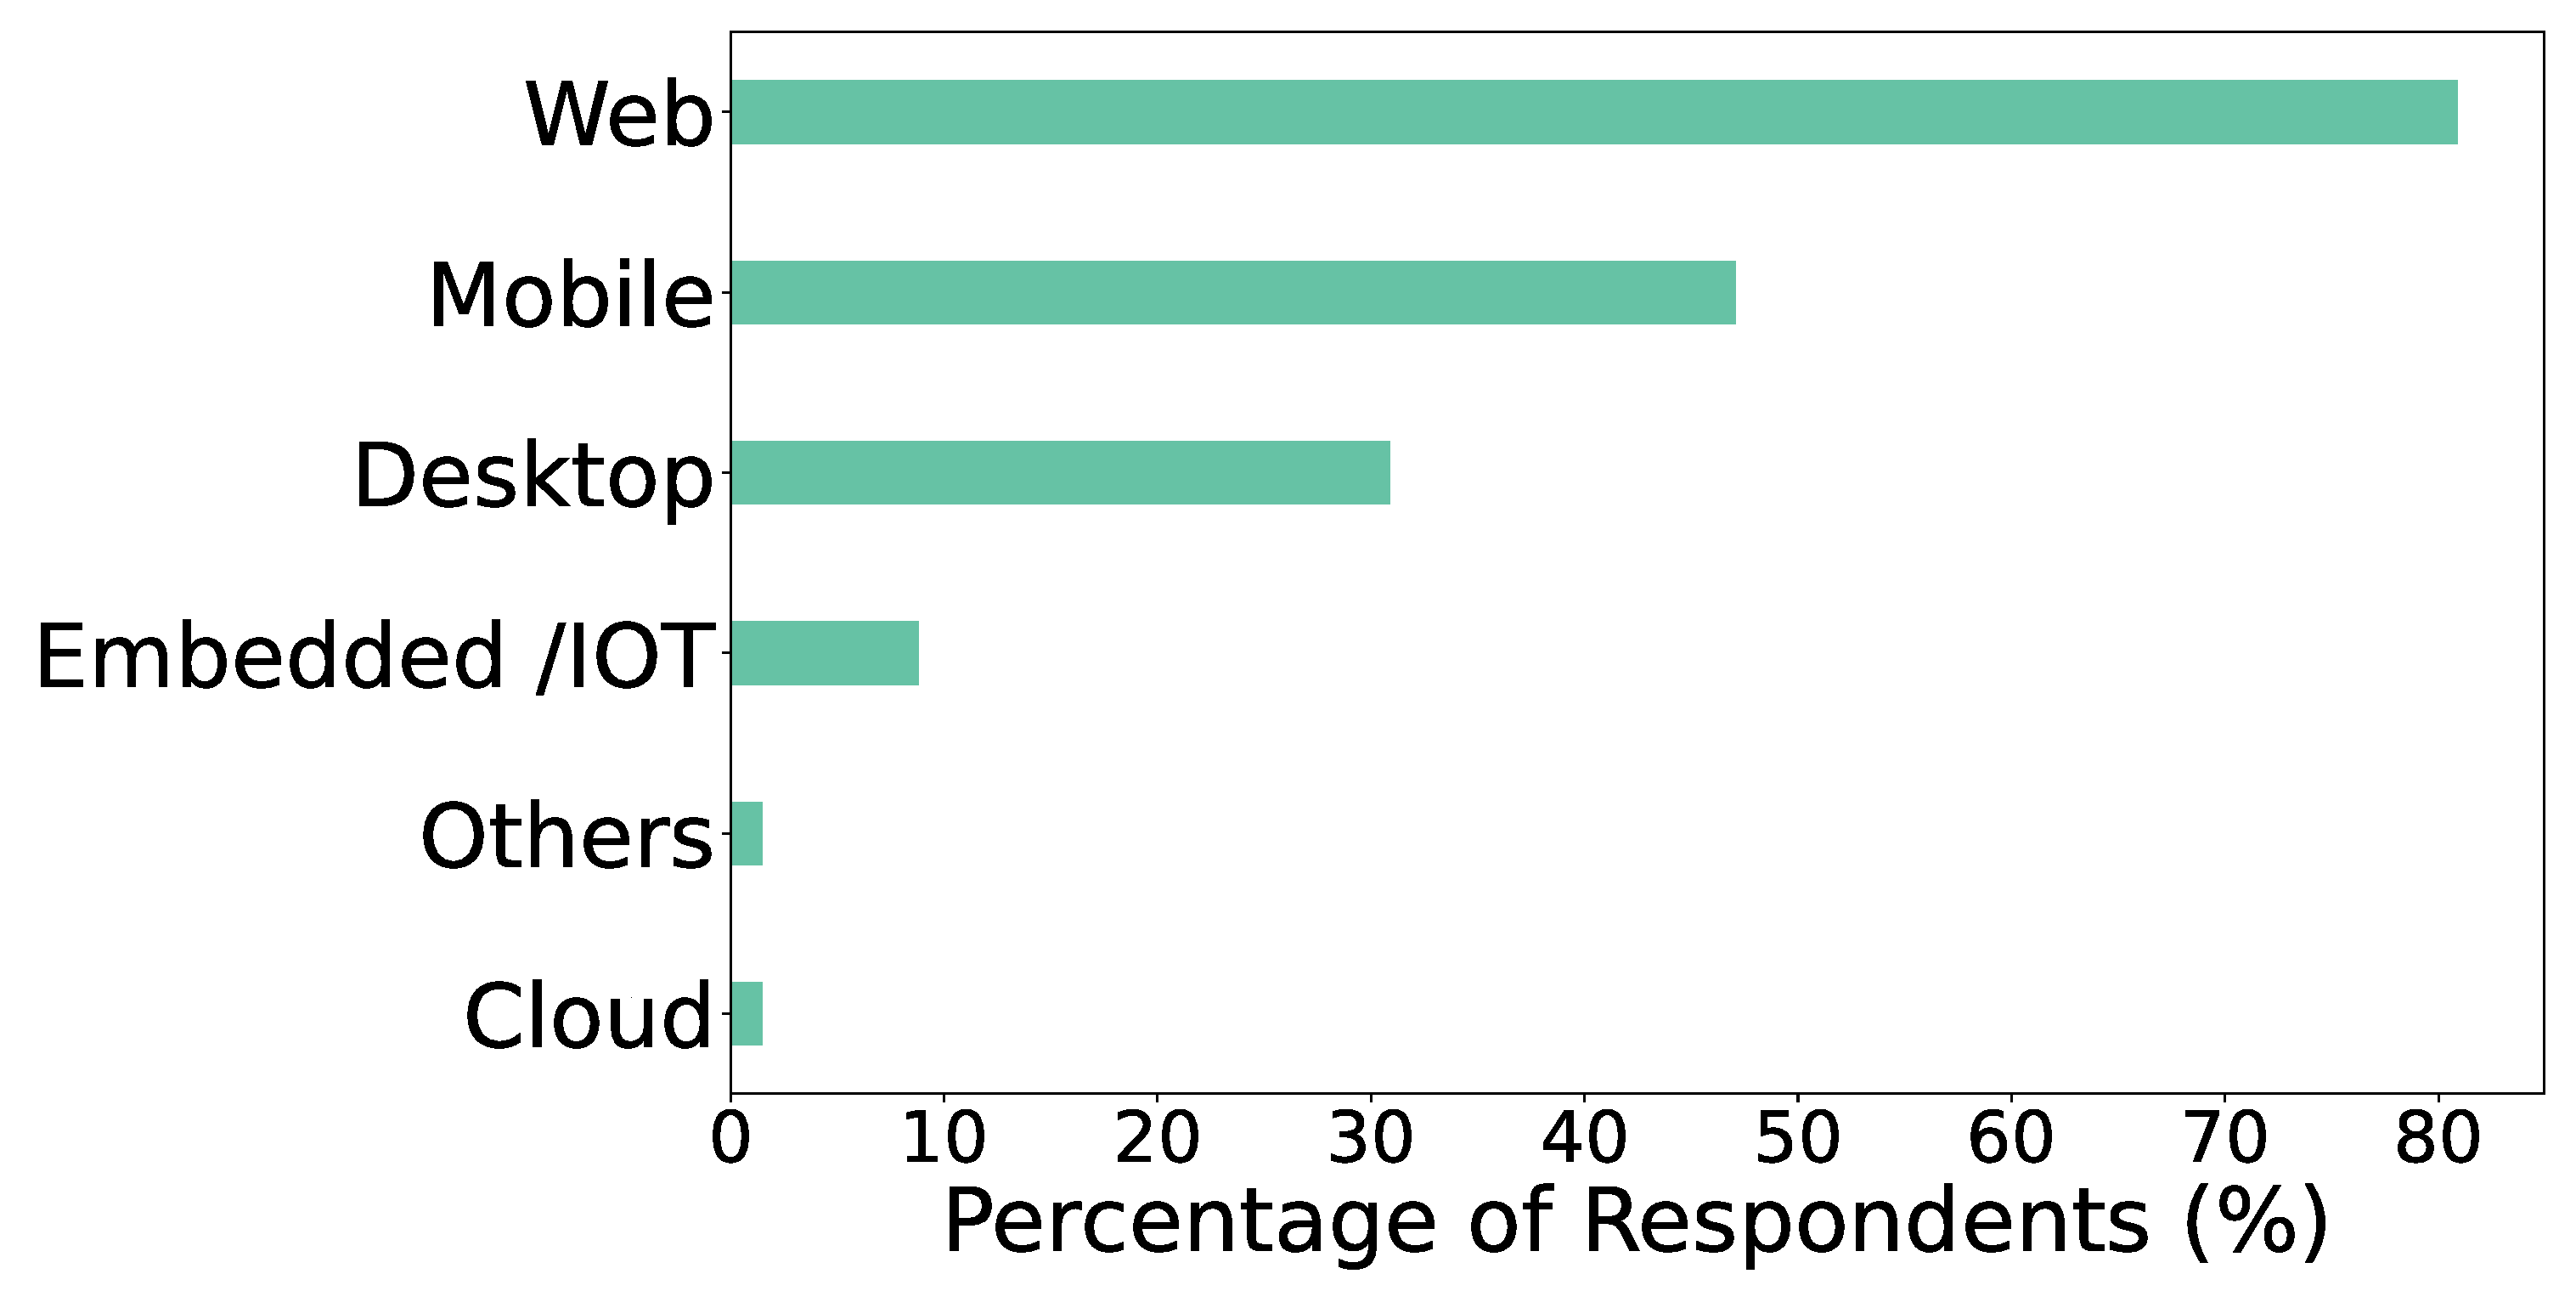
\includegraphics[scale=0.18]{Figures/Respondents_Technologies}
  \caption{Technology Platforms}
  \label{fig:platforms}
\end{figure}
\begin{figure}[t]
\centering
  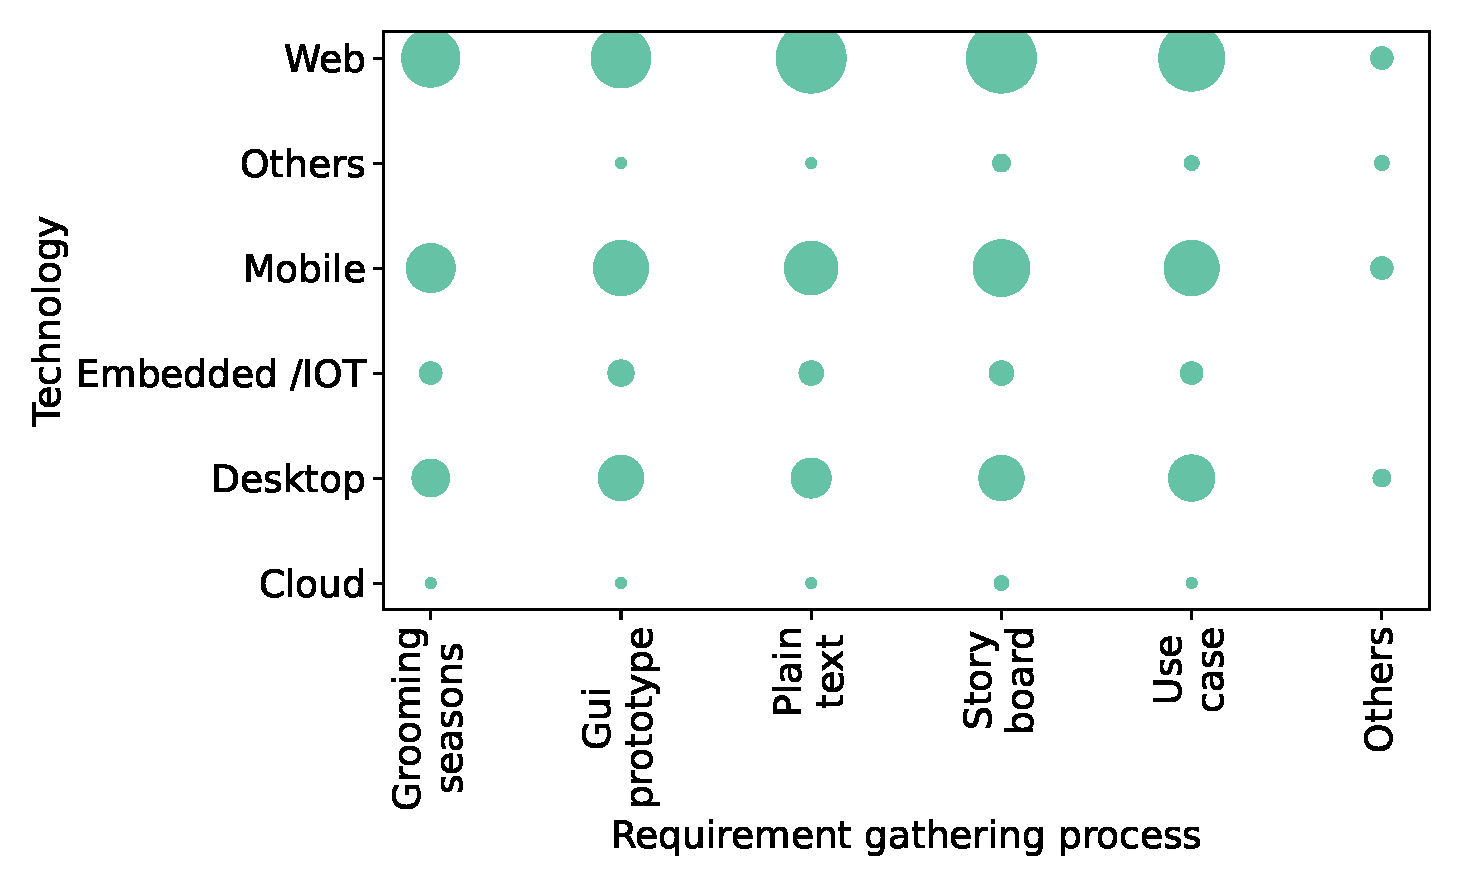
\includegraphics[scale=0.47]{Figures/Requirement_Technology_Cross_Analysis.eps}
  \caption{Cross aspect analysis of requirement gathering and technology platform}
  \label{fig:requirement technology cross analysis}
\end{figure}

%\paragraph{Operating Systems (Q10).} 

For operating systems (Q10), most of our
respondents preferred Linux based operating system (56\%) for their development (Figure \ref{fig:os}). The second frequently used
operating system is Windows (45\%) followed by MacOS (28\%). We
observed similar scenarios in the 2018 and 2019 StackOverflow (SO) surveys
\cite{StackoverflowSurvey2018,StackoverflowSurvey2019}. However, Windows ranked
first in the 2020 survey of both SO and JetBrains \cite{StackoverflowSurvey2020,
JetBrains2020}. The recent higher preference towards Windows could be due to the newly
included WSL (Windows Subsystem for Linux). This feature allows users to perform
almost any Linux-specific task on Windows. We anticipated that the use of OS
might be related to professional experience. Among the participants,
senior/expert developers (those with at least 5 years of experience) have significantly higher rates of Linux usage ($p=0.024$ based on Mann Whitney U test). 
\begin{figure}[h]
\centering
  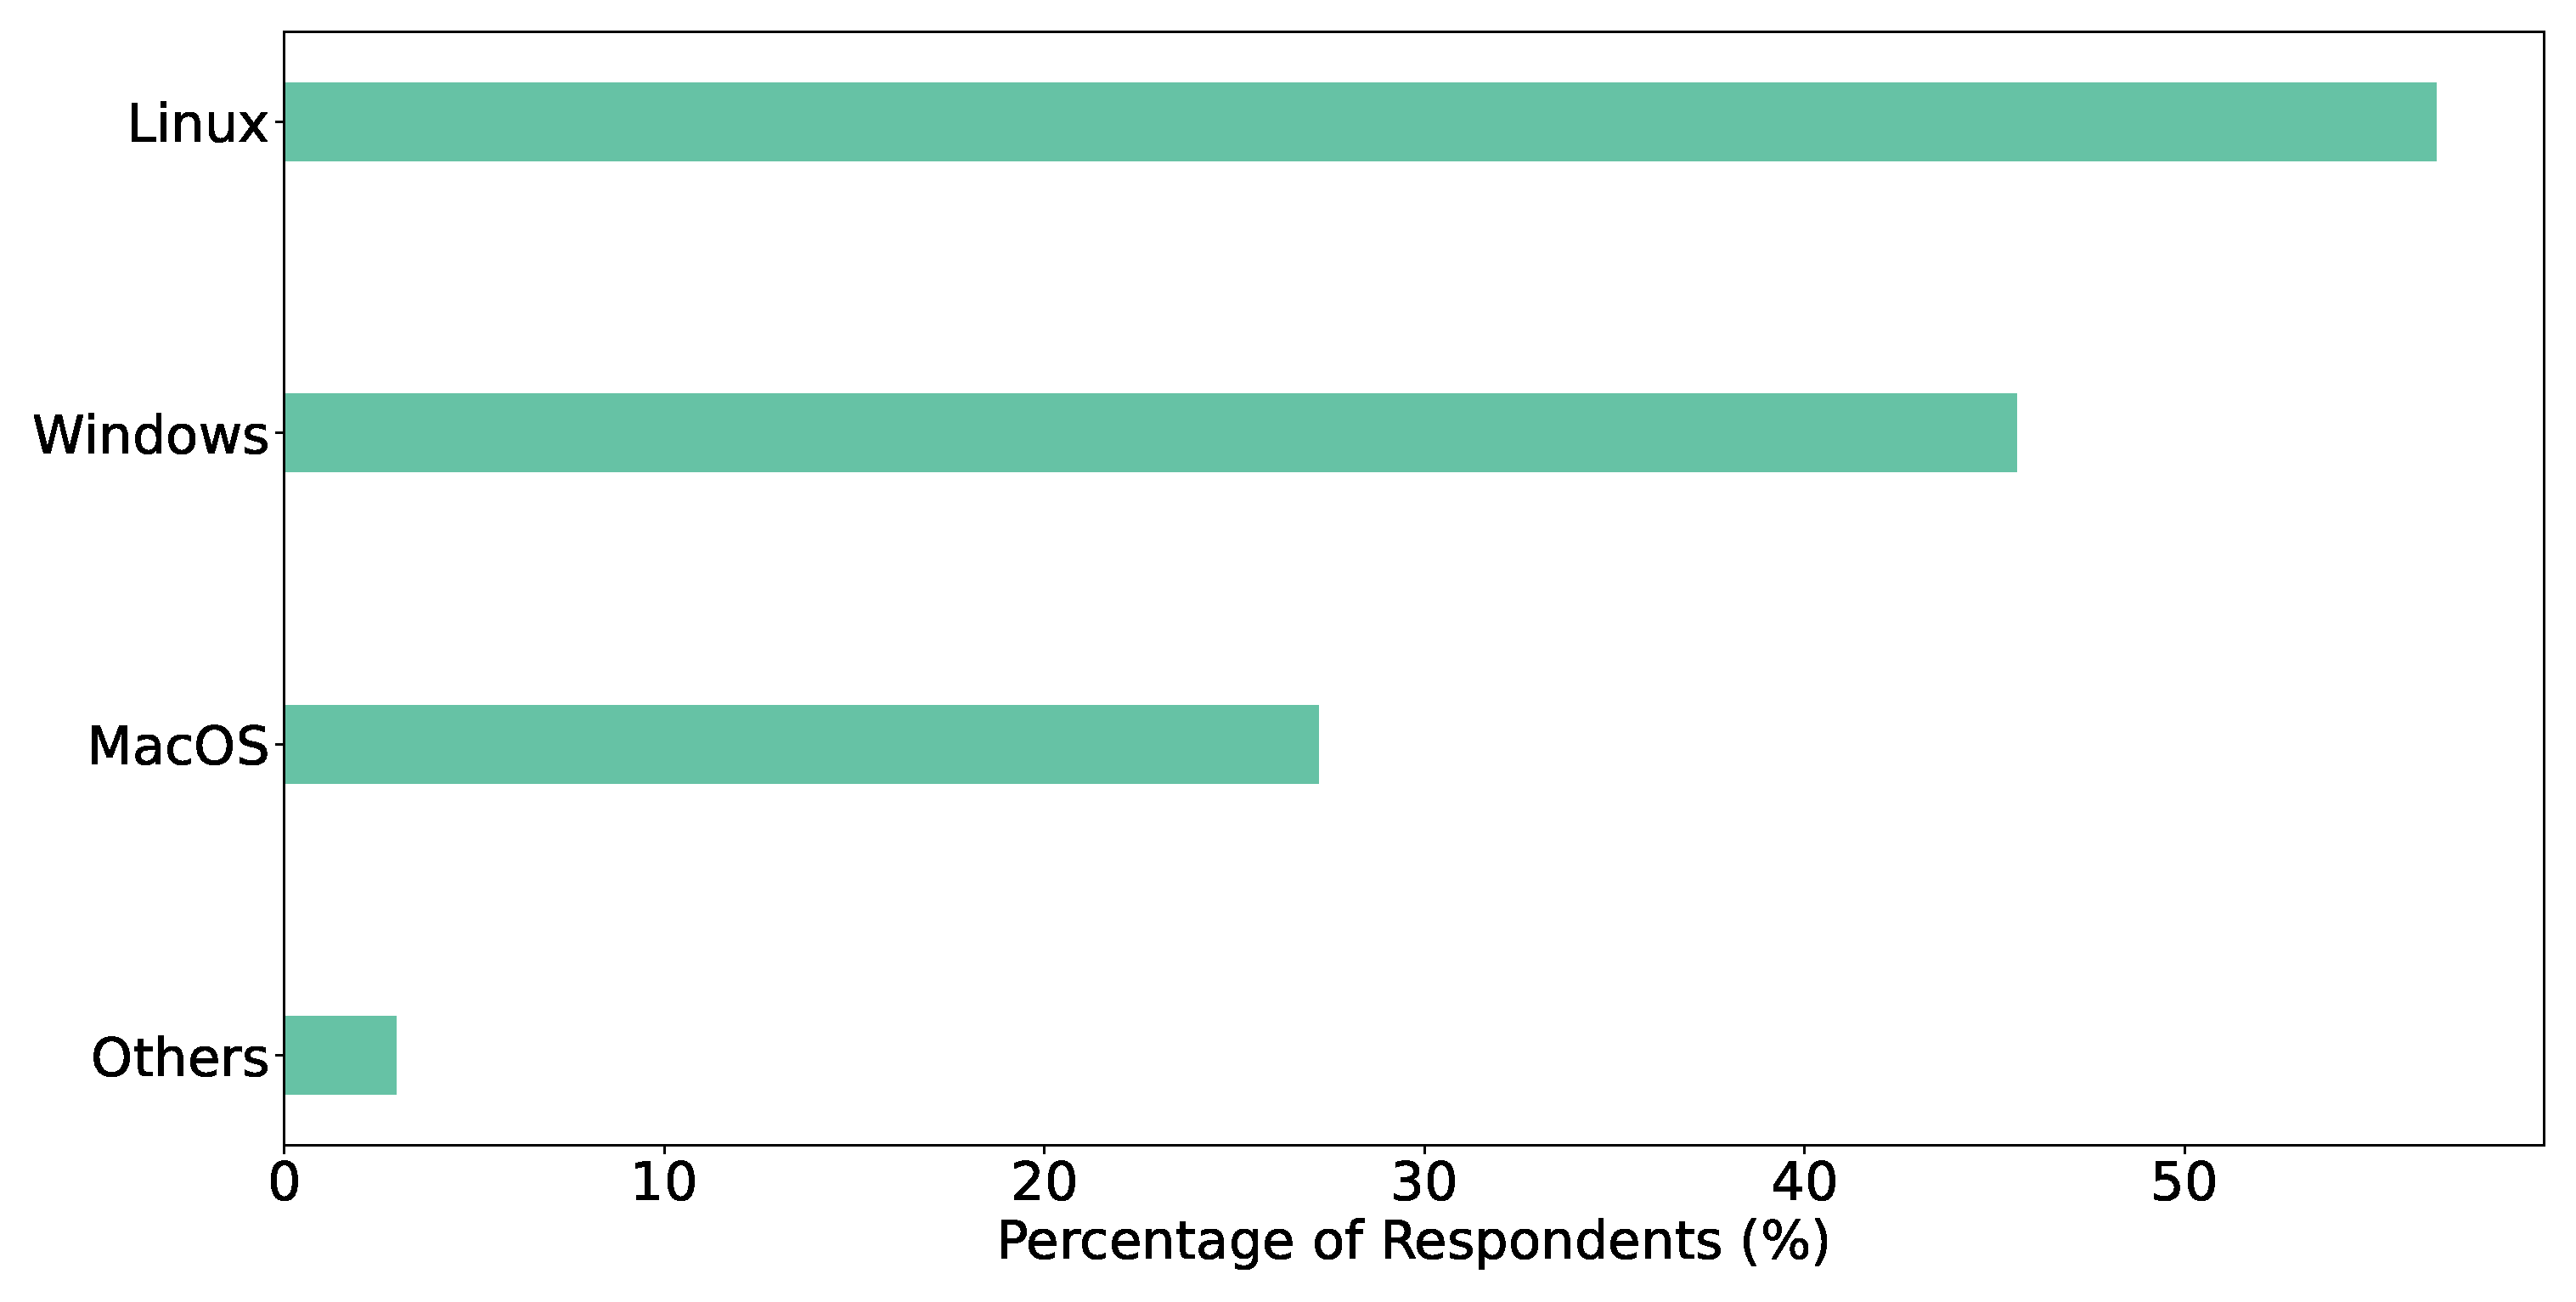
\includegraphics[scale=0.17]{Figures/Respondents_os}
  \caption{Operating Systems}
  \label{fig:os}
\end{figure}
%\paragraph{Programming Languages (Q11).} 
For programming languages (Q11), around 65\% and 60\% of our respondents use JavaScript and
Java, respectively, which are the two most used languages in Bangladesh (Figure
\ref{fig:languages}). Both JavaScript and Java are popular for web and mobile
platforms. A great percentage of our survey participants develop for both
web and mobile platforms. Other languages
like PHP (25\%), Python (25\%), and C\# (18\%) are also used, which indicates
that the software engineers are not biased towards a single specific language.
Our survey result matches with the last two years' Stack Overflow survey and the
GitHub stat. In all of the cases, JavaScript is the most used language, followed
by Java and Python \cite{StackoverflowSurvey2020, StackoverflowSurvey2019,
GithubStat}. We
observed that users using mobile and web platforms mostly use Java and
Javascript as programming languages. However, this is not statistically
significant ($p=0.1$). Though the use of the operating system can be influenced by
programming language (e.g., Swift and macOS), we do not find any significant correlation
between the two choices.
\begin{figure}[t]
\centering
  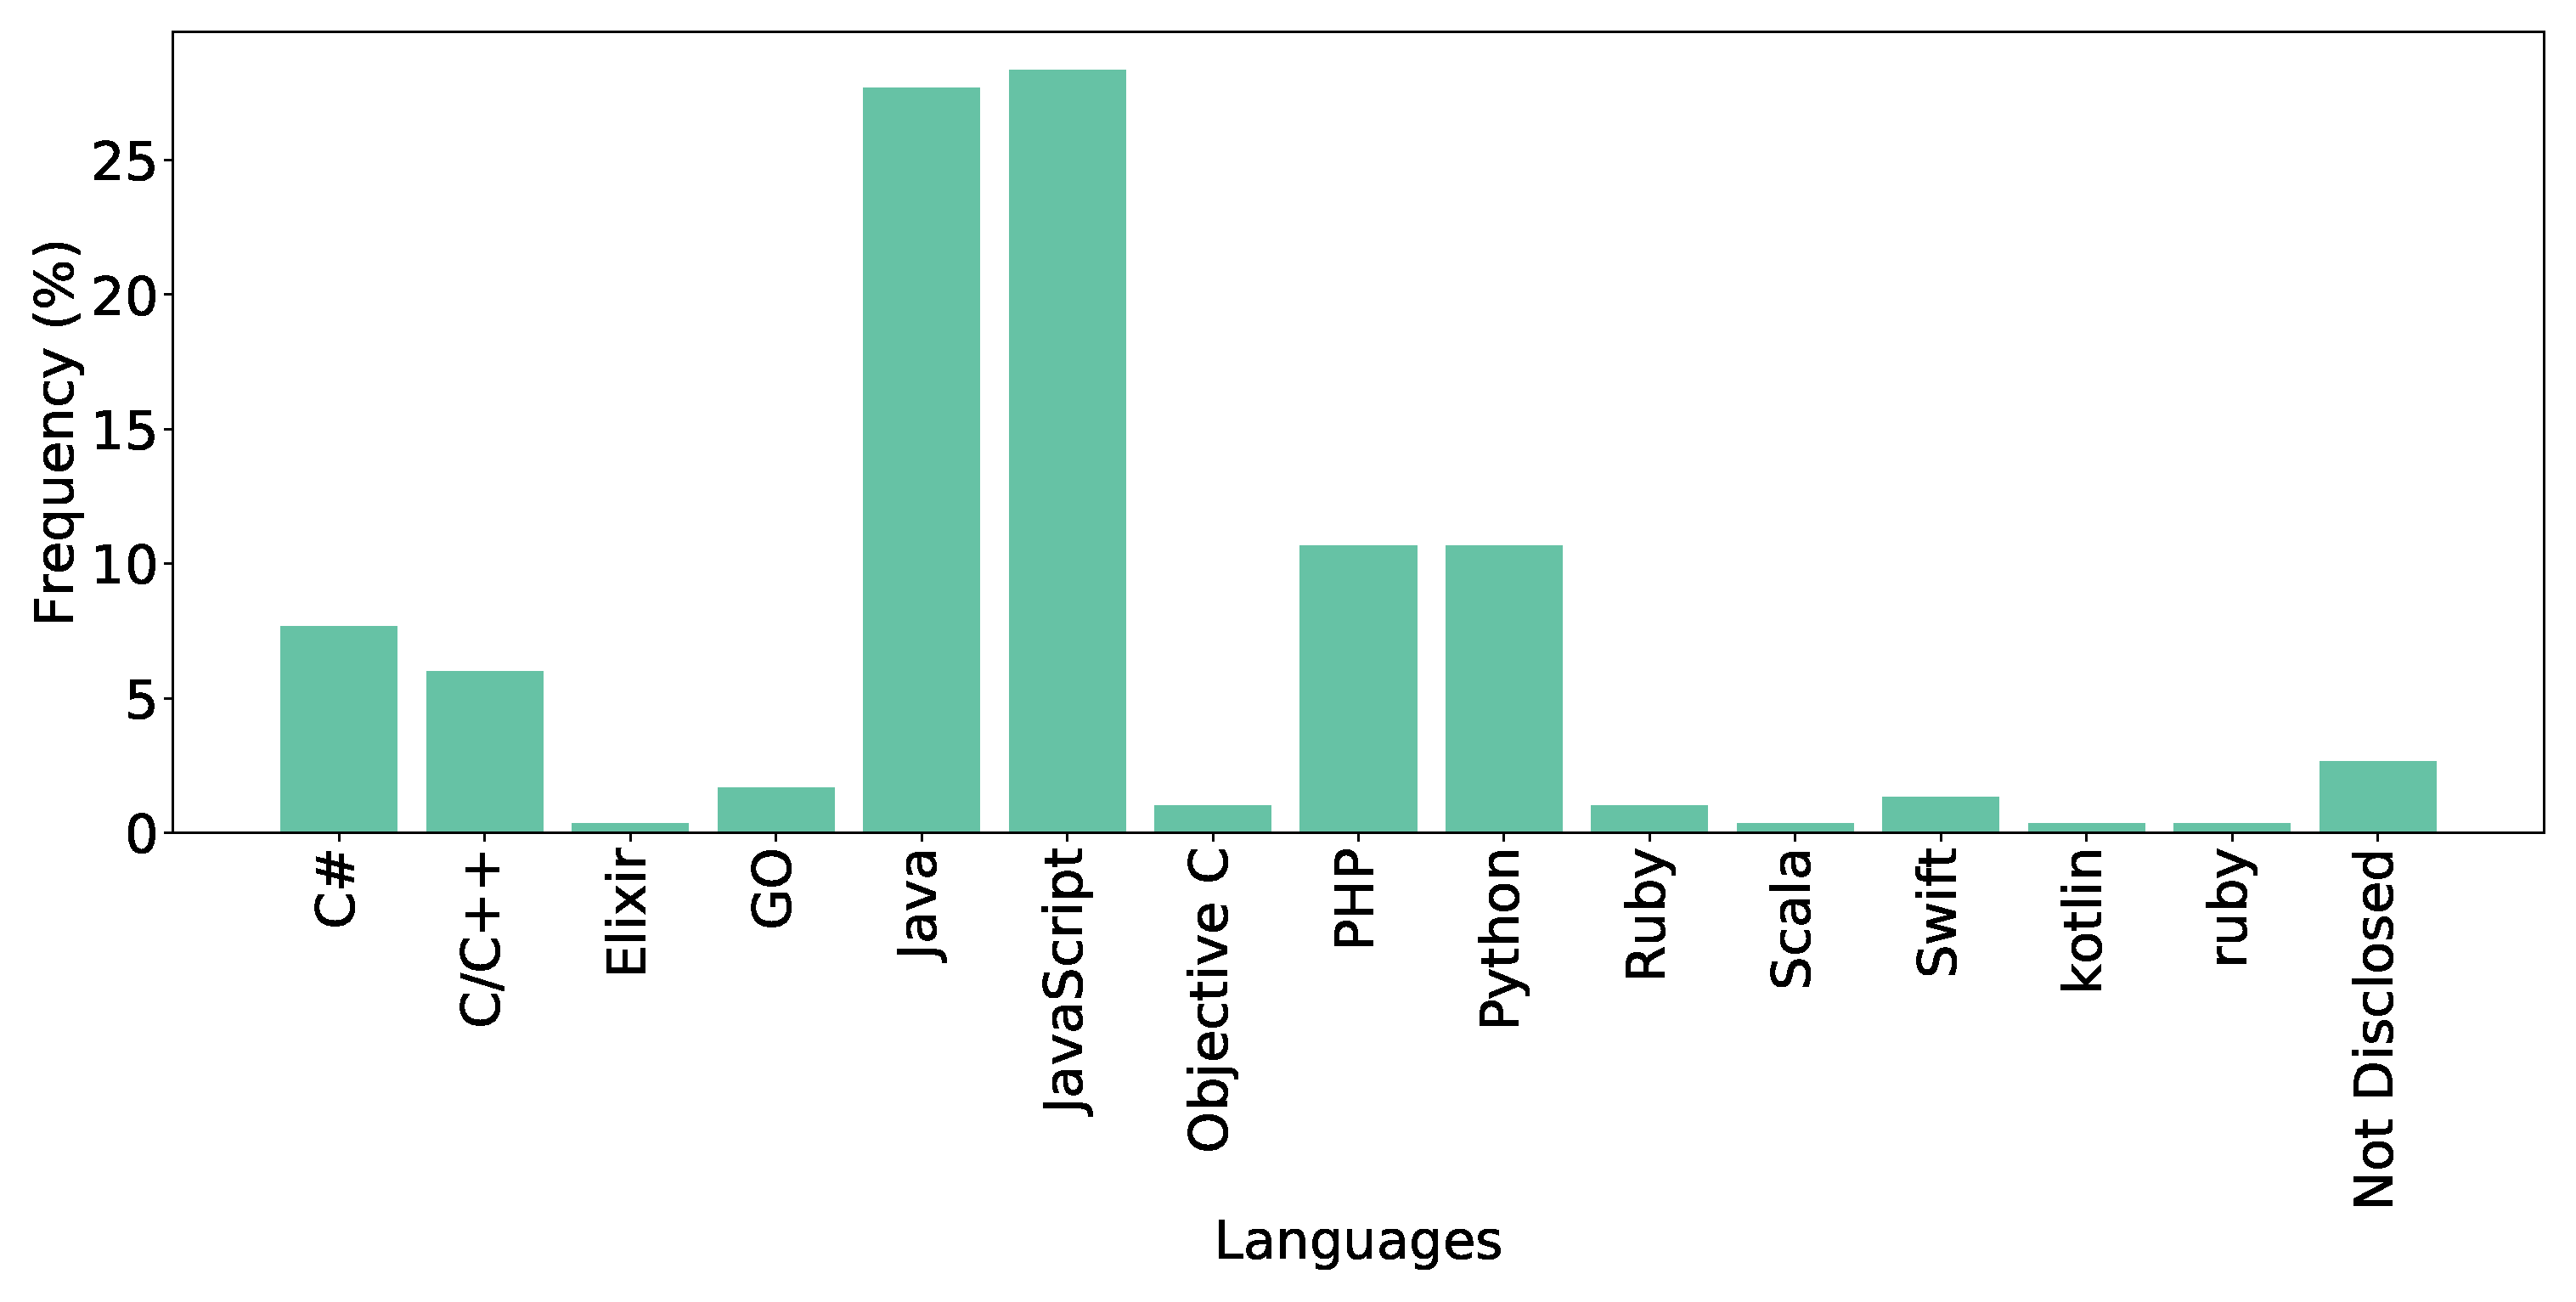
\includegraphics[scale=0.18]{Figures/Respondents_languages}
  \caption{Languages used in software development}
  \label{fig:languages}
\end{figure}

%\paragraph{Frameworks used in development}
For frameworkes used in development (Q12), as shown in Figure \ref{fig:frameworks} Spring boot (37\%) is the most used framework in the Bangladesh software industry. 
This observation is aligned with the result of Java's usage rate corresponding
to Figure \ref{fig:languages}. Since JavaScript is the most used language of our
respondents, they use various JavaScript frameworks such as React, Node.js,
Angular, Express, etc. ASP.NET, Django, and
Laravel are used in the same proportion based on around 15\% of our respondents.
React, Swift, Ruby on Rails, Node.js, etc., are comparatively less used. Other
than these, lots of frameworks such as Cocoa, Meteor, TestNG, Relay, Appium,
CakePHP, etc., are also used (presented as `Others' in Figure \ref{fig:frameworks}). For web development, Django
and Spring frameworks are mostly used in Bangladesh ($p=0.04$). We have compared
our results with the Stack Overflow 2016 to 2020
survey\cite{StackoverflowSurvey2017, StackoverflowSurvey2018,
StackoverflowSurvey2019, StackoverflowSurvey2020}. The only common framework in
the top five list in both surveys is ASP.NET. In the stack overflow survey, we
noticed that JavaScript-based frameworks (e.g., Jacqueline, Angular, React,
Node.js) occupy the top positions (top five), which is not the case for our
survey.

\begin{figure}[t]
\centering
  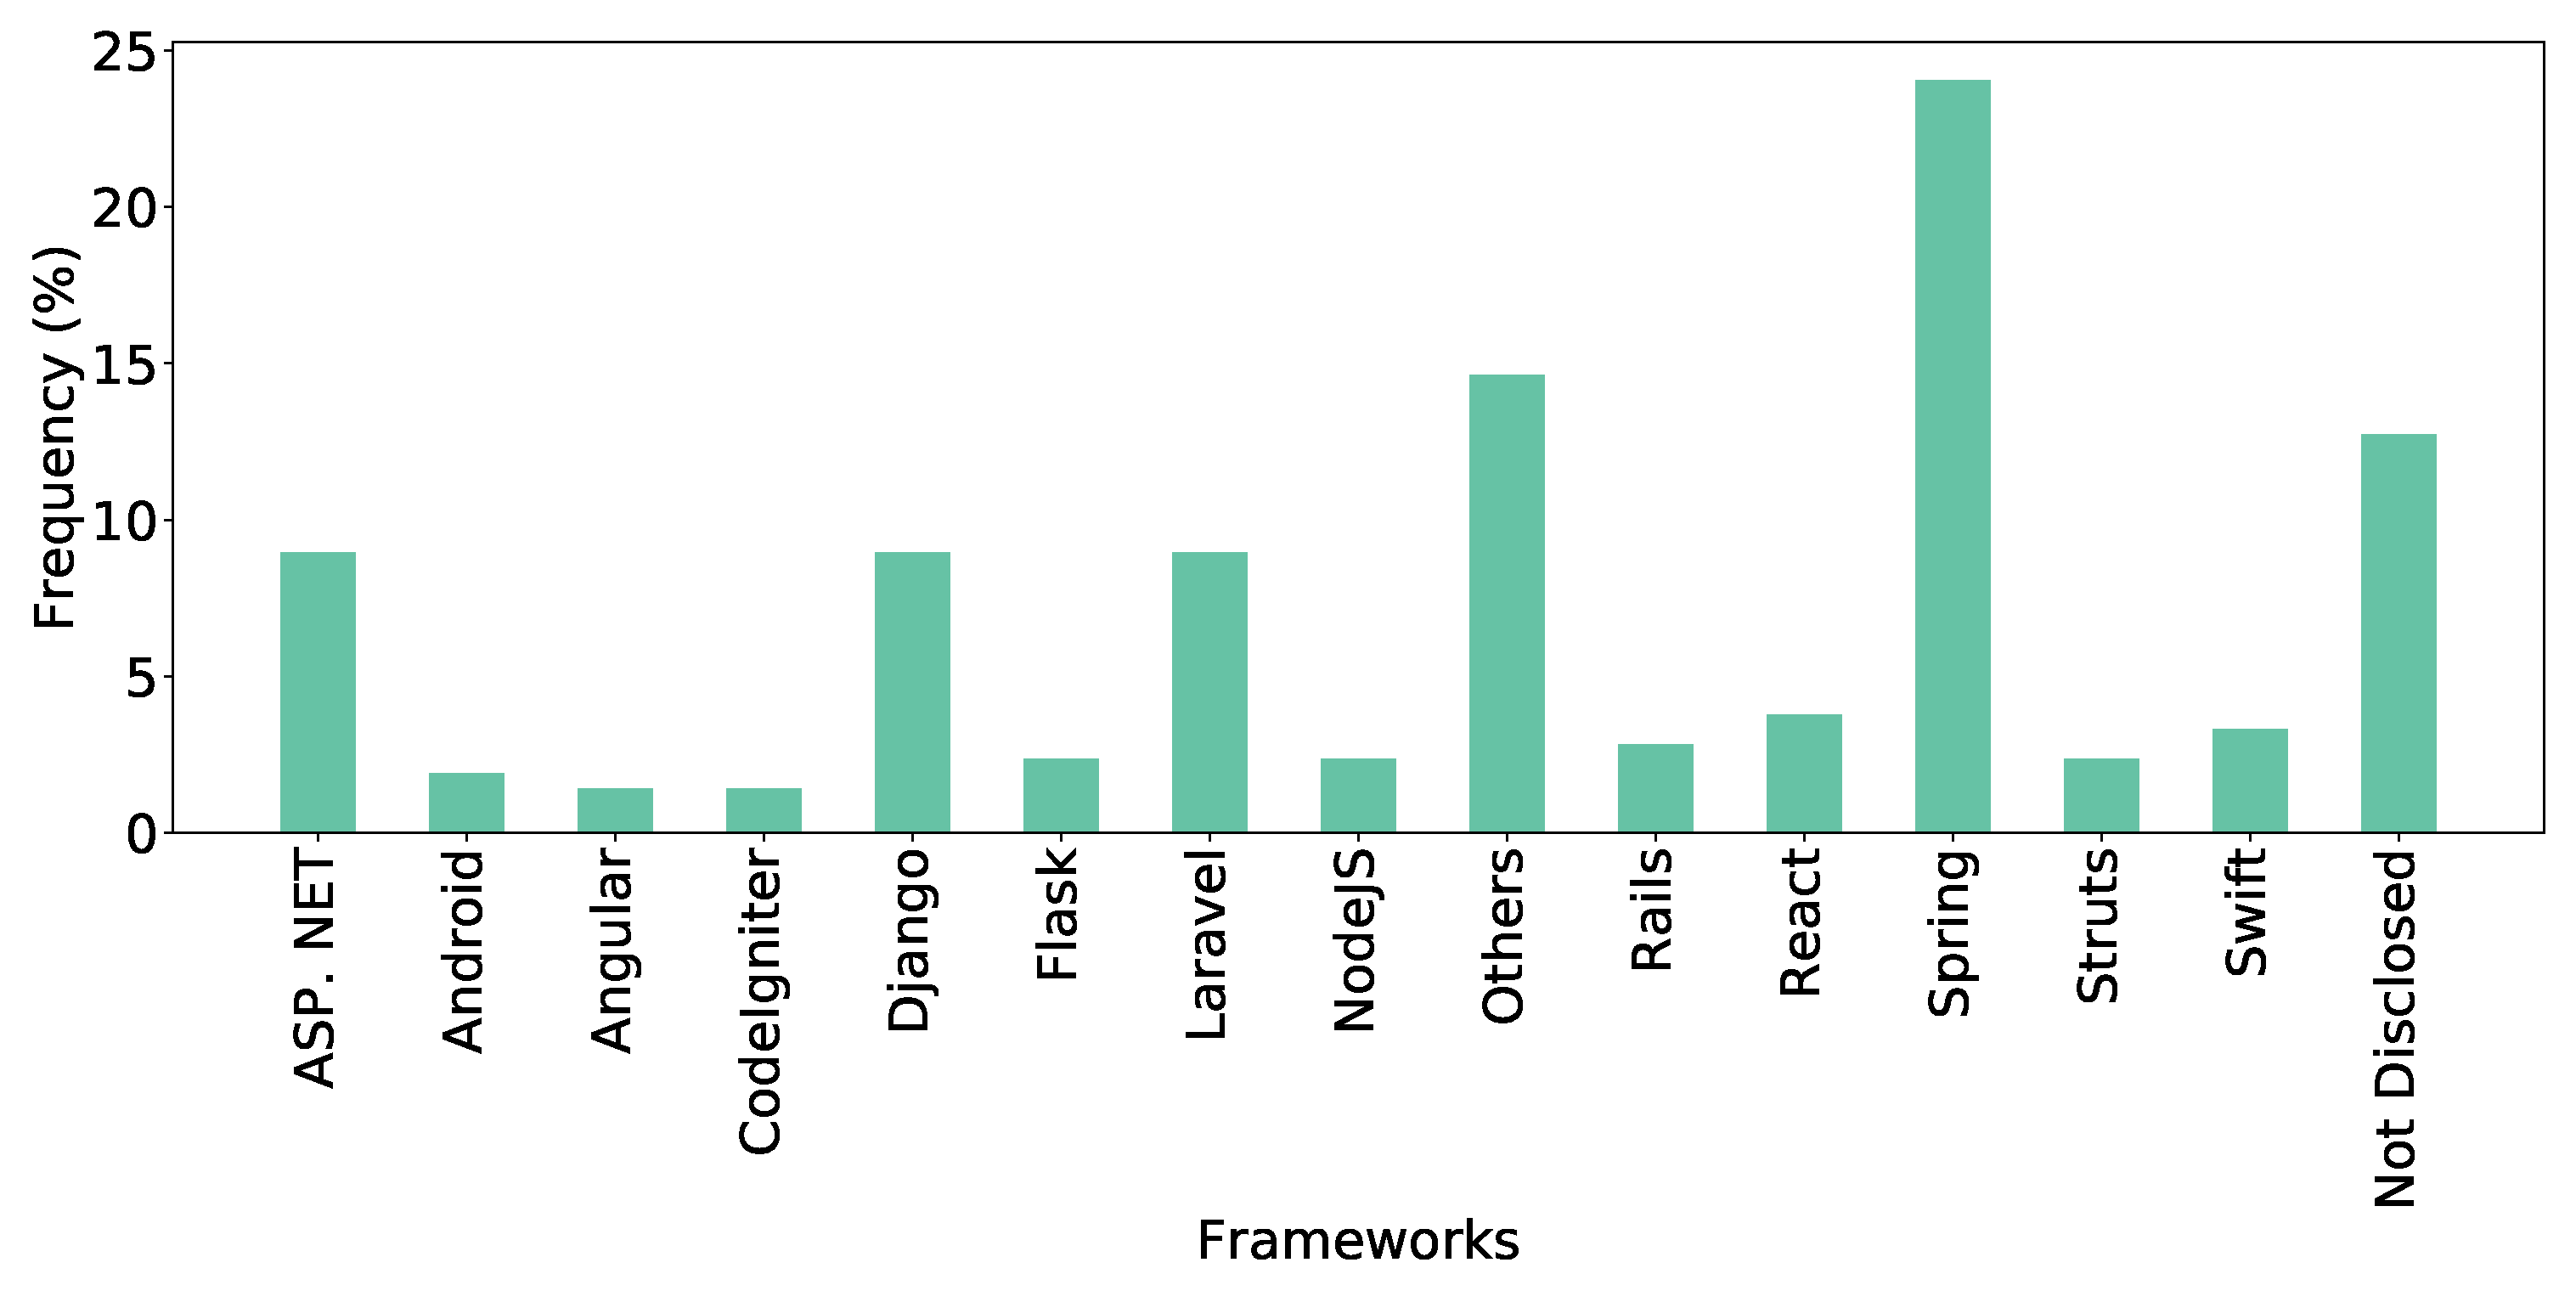
\includegraphics[scale=0.18]{Figures/Respondents_frameworks}
  \caption{Frameworks}
  \label{fig:frameworks}
\end{figure}

%\paragraph{IDE's used by the respondent's} 
Among the IDEs (Q13), as shown in Figure \ref{fig:IDEs},
IntelliJ, is used by most respondents (43\%). IntelliJ is a Java integrated development tool for developing software for the
enterprise, mobile, and web application, The
other IDEs used in SE industries are Visual Studio (30\%), Eclipse (24\%),
PyCharm (17\%), NetBeans (11\%), and Android Studio (7\%).

\begin{figure}[t]
\centering
  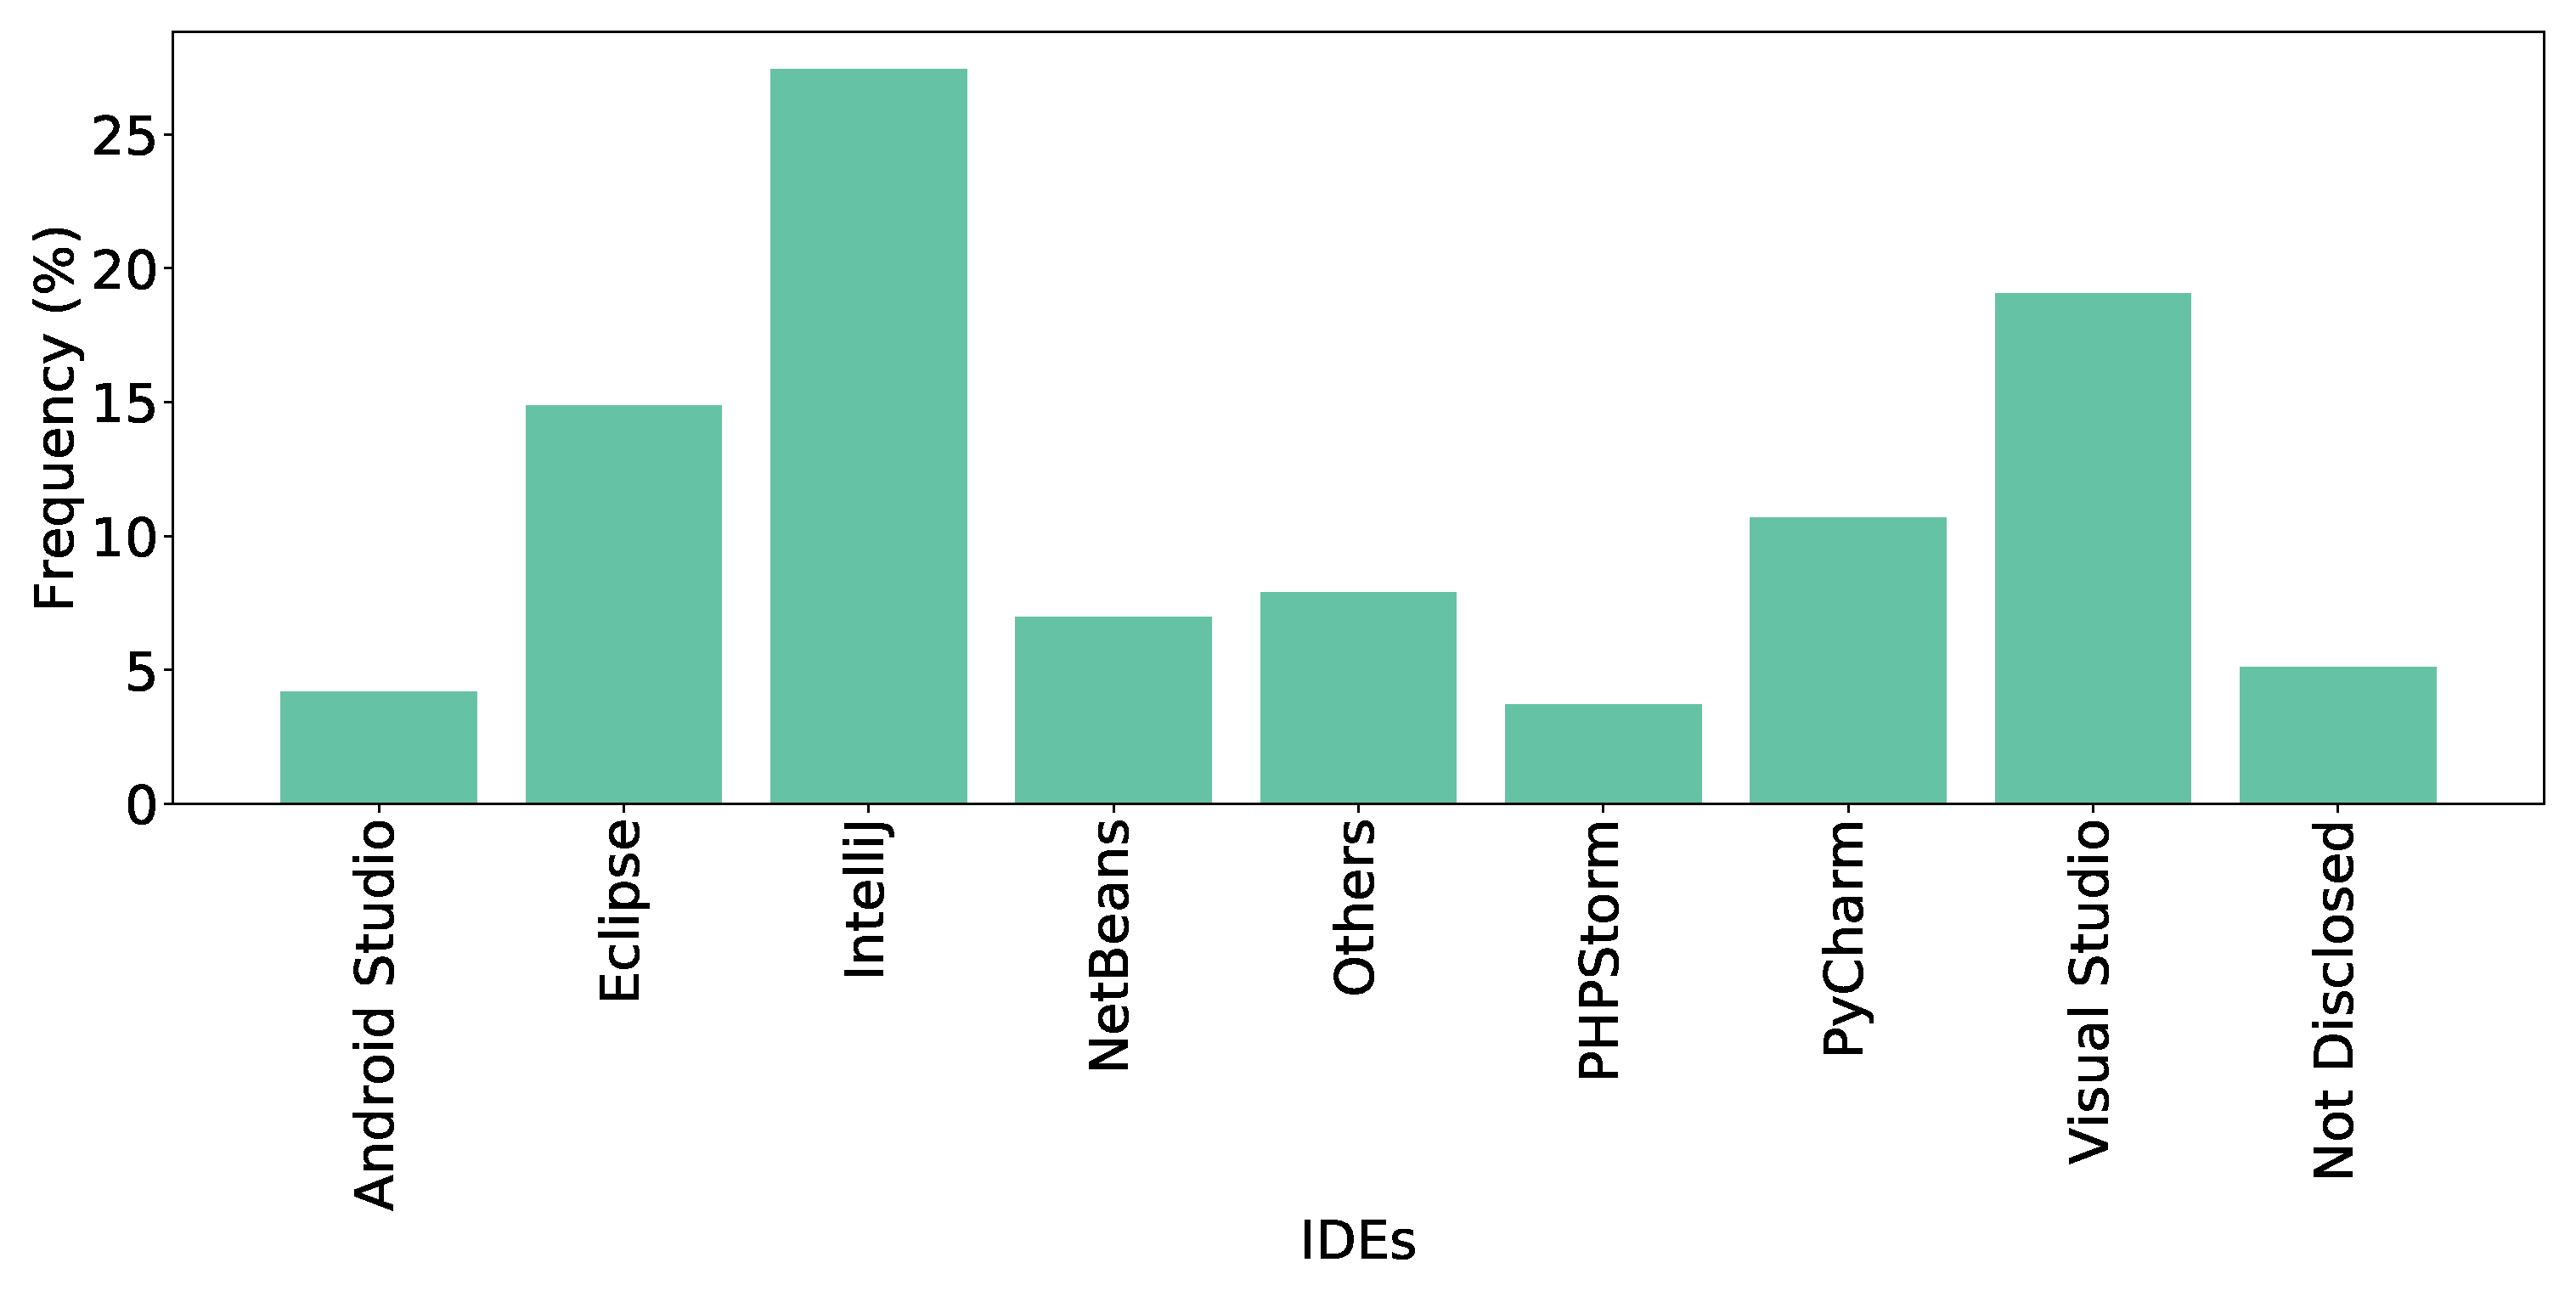
\includegraphics[scale=0.18]{Figures/Respondents_IDEs}
  \caption{IDE's}
  \label{fig:IDEs}
\end{figure}
\begin{tcolorbox}[flushleft upper,boxrule=1pt,arc=0pt,left=0pt,right=0pt,top=0pt,bottom=0pt,colback=white,after=\ignorespacesafterend\par\noindent]
\nd\it{\bf{RQ1-D2. Software development tools and techniques used.}} Web based software services top the list of development technologies. Requirement gathering process is mostly practiced in GUI-based development
(e.g., web, desktop, mobile) \gias{summarize findings from Q10-13 also here}
\end{tcolorbox}
% \boxtext{Web based software services top the list of development technologies. Requirement gathering process is mostly practiced in GUI-based development
% (e.g., web, desktop, mobile) \gias{summarize findings from Q10-13 also here}}

\subsubsection{What type of testing and deployment practices are used?}
\label{testing_practices}

Testing is an important process in improving the quality of the software product. The purpose of this process is to find errors, which might occur during specification, design, and code generation. We report the following results next:
\begin{itemize}
\item Software Testing Practices (Q 14)
\item Level of Automated Testing (Q 15)
\item Tools Used in Testing and QA (Q 16)
\item Continuous Deployment tools (Q 17)
\item Version Control (Q 18)
\end{itemize}


\paragraph{Software Testing Practices}
According to Figure \ref{fig:testing}, several numbers of testing practices are used during software development. The results show that most of the organizations have carried out unit testing (53\%), functional testing (49\%), user acceptance testing (39\%), GUI testing (31\%), etc. Unit testing also ranked first in the 2019 survey of JetBrains, where it was voted by 71\% participants across the globe \cite{JetBrains2019}. We observed in our survey that in some cases managers have reported to perform GUI testing and performance testing, which is unlikely due to their role/designation. However, the observation is not statistically significant ($p=0.12$). It may be deduced that in absence of enough specialized resource managers have to take additional responsibility. To identify the relation between testing practices and experience, we plotted them together in Figure \ref{fig:testing type and experience}. In Figure \ref{fig:testing type and experience}, we observed that junior developers mostly perform unit, integration, and functional testing, whereas senior developers mostly perform API testing. We conducted the Mann Whitney U test to assess the conjecture, and it is found statistically significant ($p$<$0.01$).
\begin{figure}[h]
\centering
  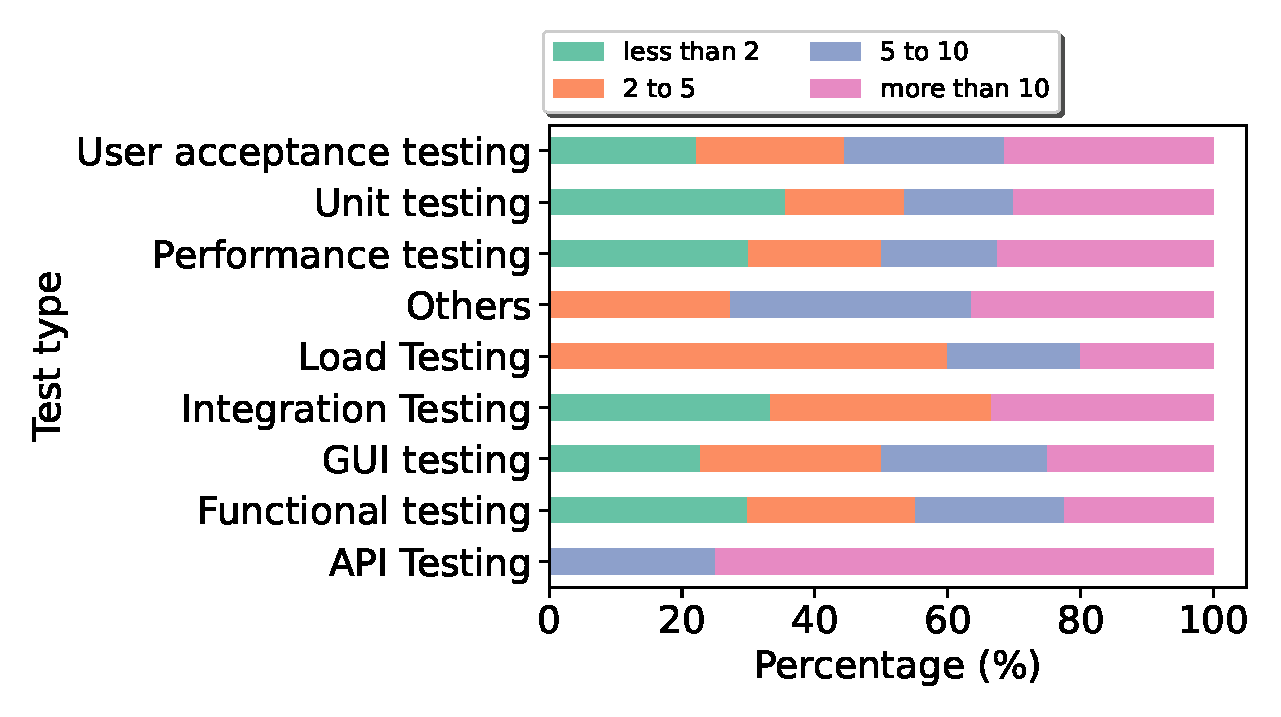
\includegraphics[scale=0.6]{Figures/Testing_Type_and_Experience}
  \caption{Testing practices ans professional experience}
  \label{fig:testing type and experience}
\end{figure}

\begin{figure}[h]
\centering
  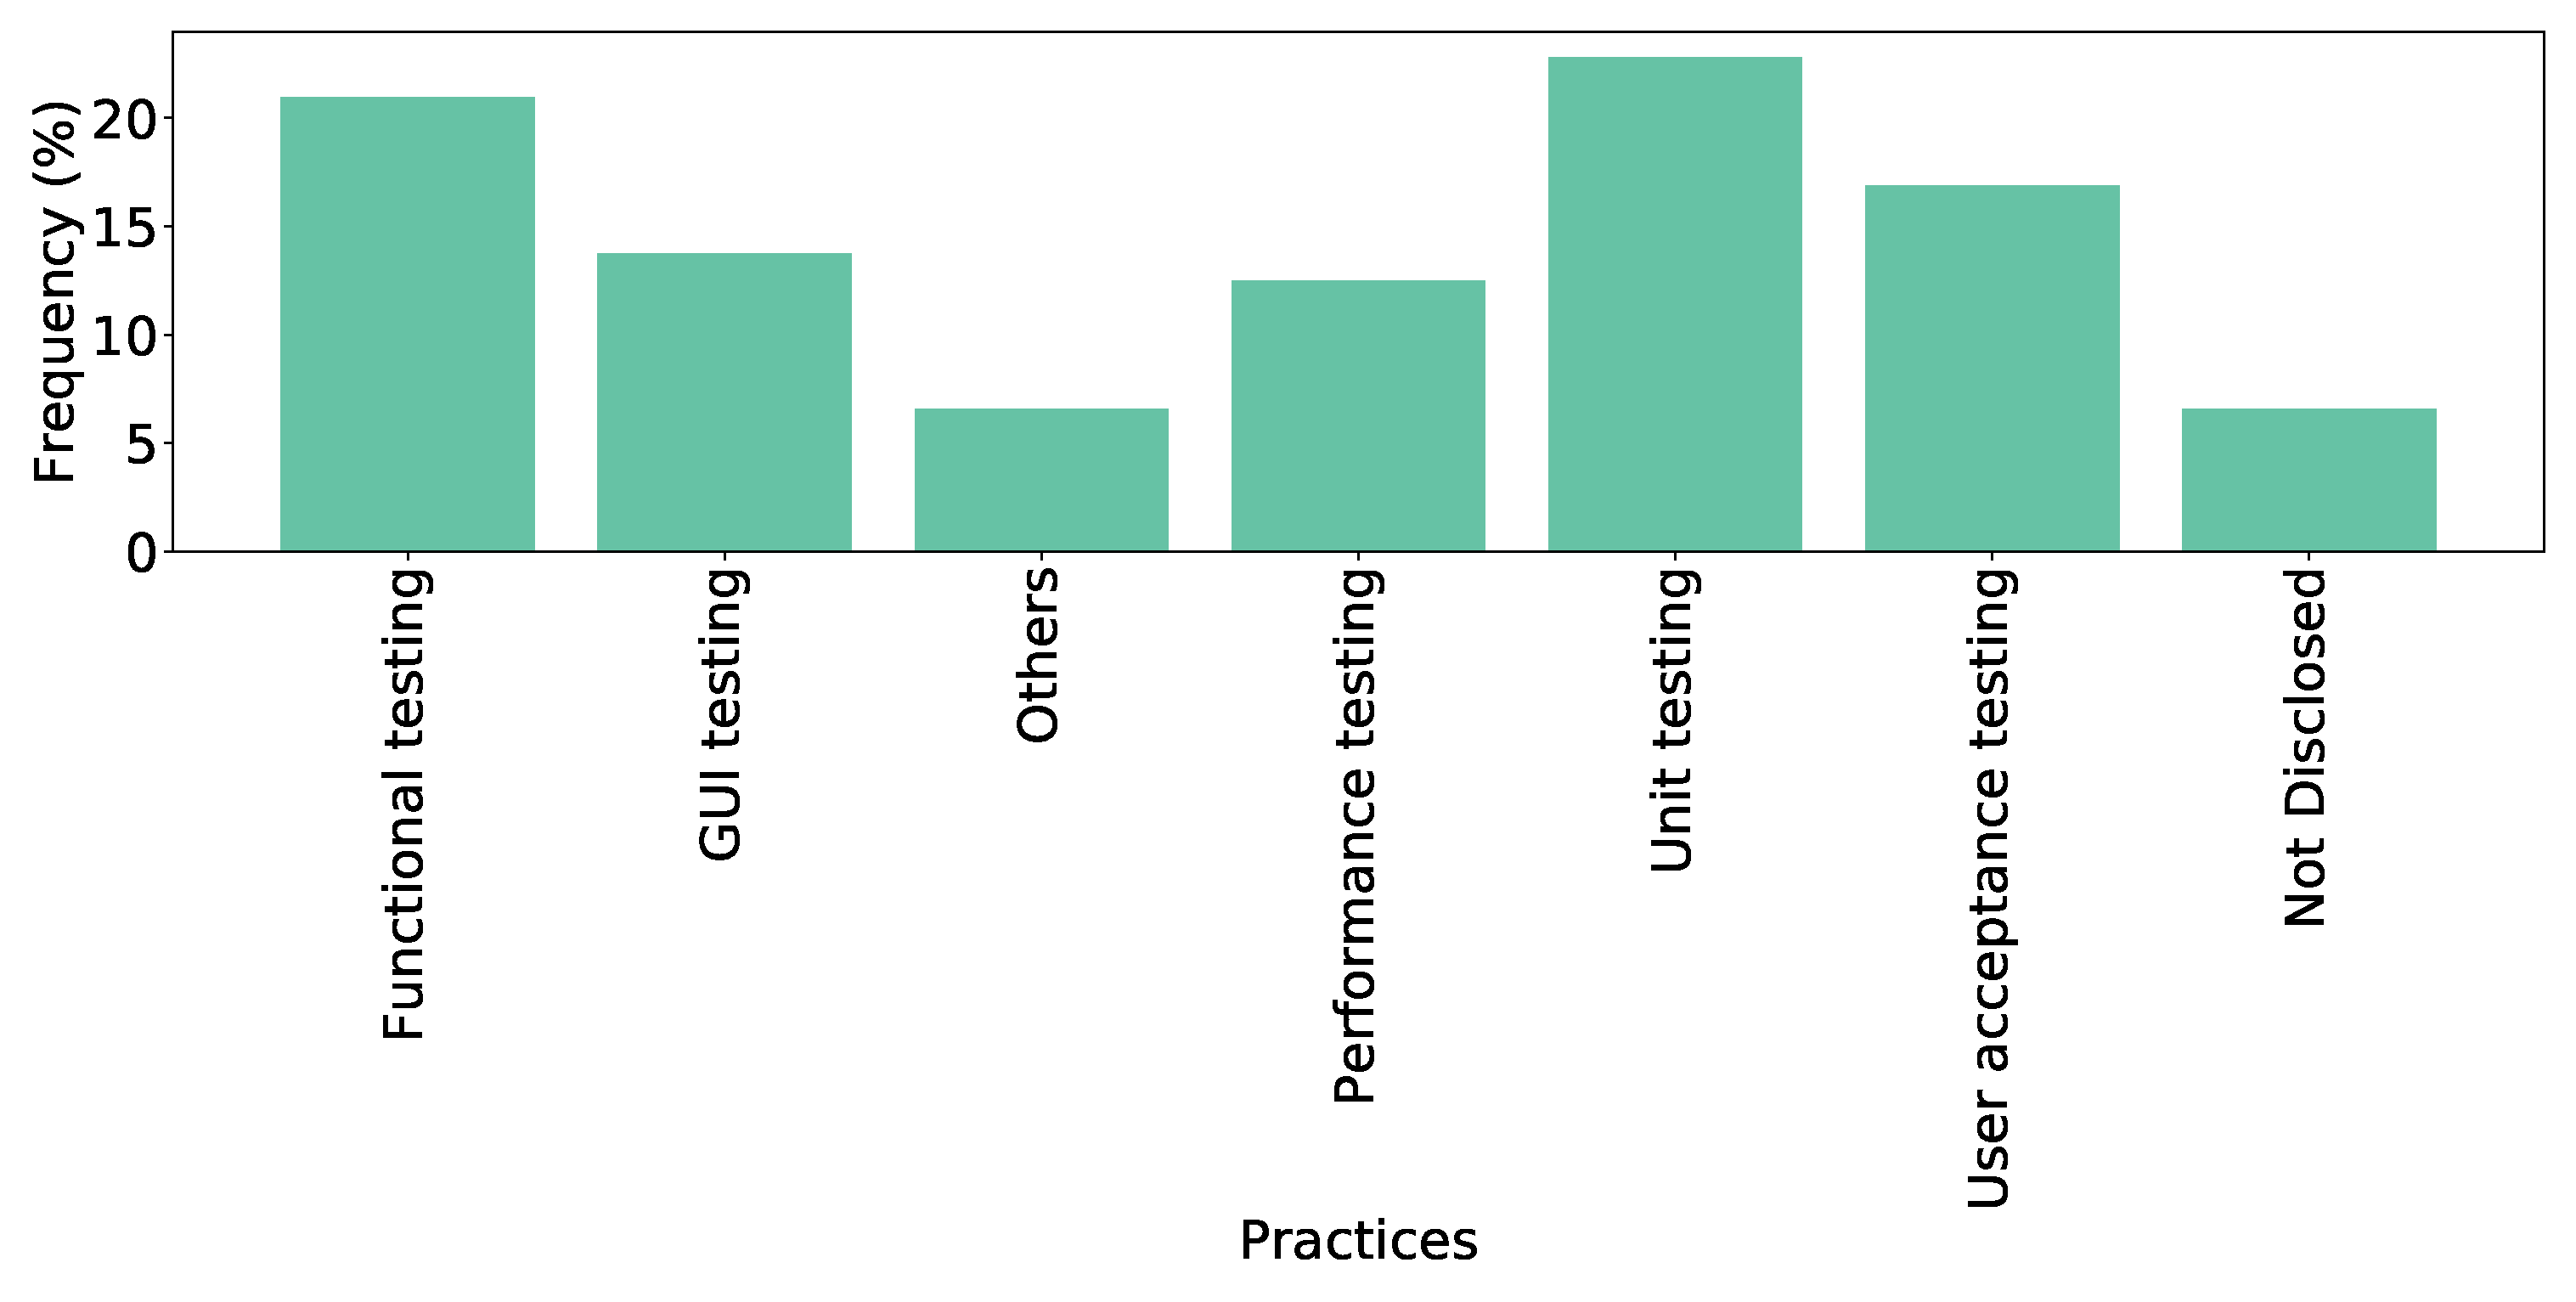
\includegraphics[scale=0.2]{Figures/Respondents_testing_practices}
  \caption{Testing Practices}
  \label{fig:testing}
\end{figure}


\paragraph{Level of Automated Testing}
Question 15 asked about the level of automated testing  performed in the company. The responses were gathered using the Likert scale. It was found that different respondents have very different experience in this context, i.e., some companies heavily practice automated testing, while others favor manual testing.  Results are shown in Figure \ref{fig:autoTest} which indicates that about 70\% of our respondents (others than who voted for level 5) do not use automated testing regularly. The level of automated testing might be related to the programming language/framework. The testing suite provided by framework/language might encourage developers to implement automated testing. The level of automated testing vs language and framework is plotted in Figures \ref{fig:language and autotest} and \ref{fig:framework and autotest}, respectively. It seems from Figure \ref{fig:language and autotest} that the highest level of automated testing is mostly practiced in Java, Javascript, Objective-C, and Php language. We conducted the Mann Whitney U test to assess our conjecture and it is found statistically significant ($p=0.01$). From Figure \ref{fig:framework and autotest}, we found that the highest level of automated testing is mostly performed in Android, Express, NodeJS, Struts, and Java EE framework, and the observation is statistically significant ($p=0.006$). Also, the highest level of automated testing is mainly used by developers (mostly use unit testing), and managers practice the lowest level of automated testing. The reason why managers use the lowest level of automated testing may be related to the type of testing they perform. We observed that managers mainly engaged in assessing the acceptability of the product from the end-user point of view. \anindya{Performance test may be automated. Thing about the previous comment. We may rather say that managers are likely to assess the acceptability from end user point of view.}\partha{updated} We guess that experience might be one of the factors that influence automated testing. Our conjecture was that senior developers might tend to use more automated tests than junior developers. We plotted experience and automated test levels in Figure \ref{fig:experience and autotest}. However, we found the opposite scenario, i.e., junior developers tend to use more automated testing than senior developers. However, the observation is not statistically significant ($p=0.08$). One of the reasons behind this observation may be that the senior developers perform certain testings (e.g., GUI testing), which are hard to automate.

\begin{figure}[h]
\centering
  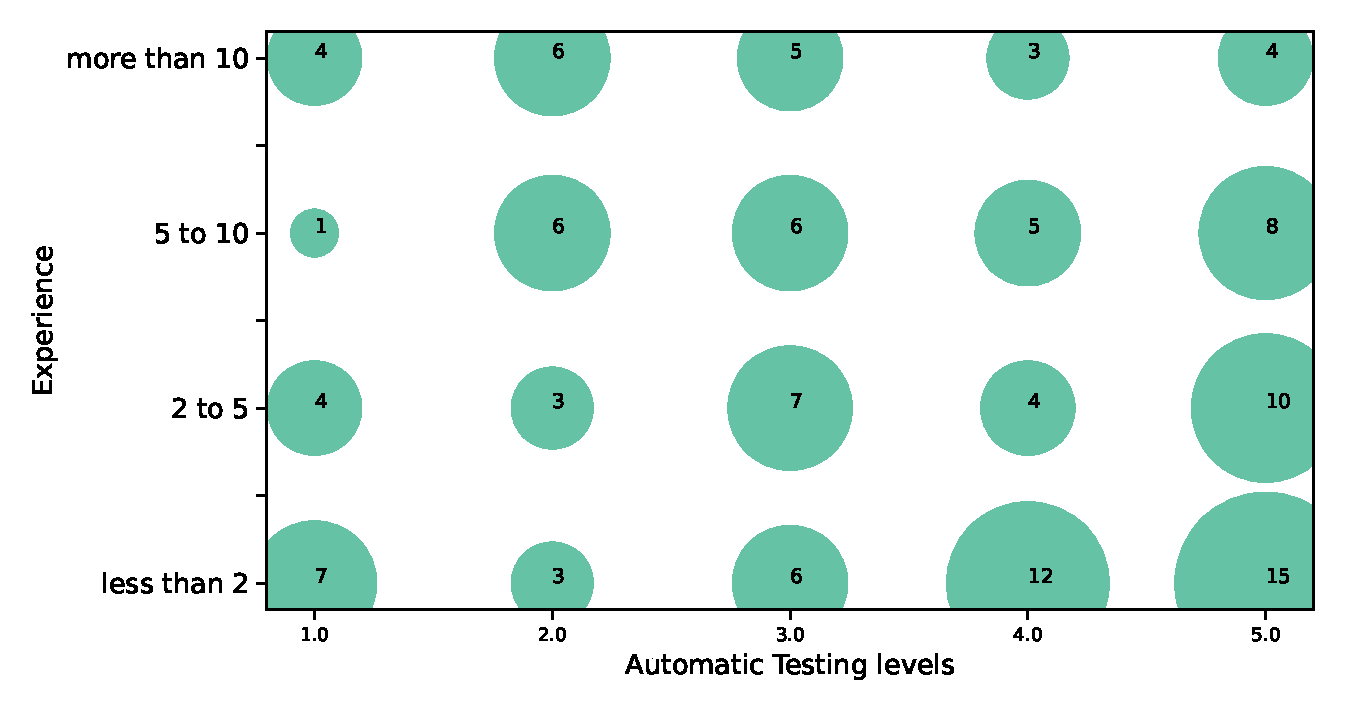
\includegraphics[scale=0.45]{Figures/Auto_Test_and_Experience}
  \caption{Experience and automated testing level}
  \label{fig:experience and autotest}
\end{figure}
\begin{figure}[h]
\centering
  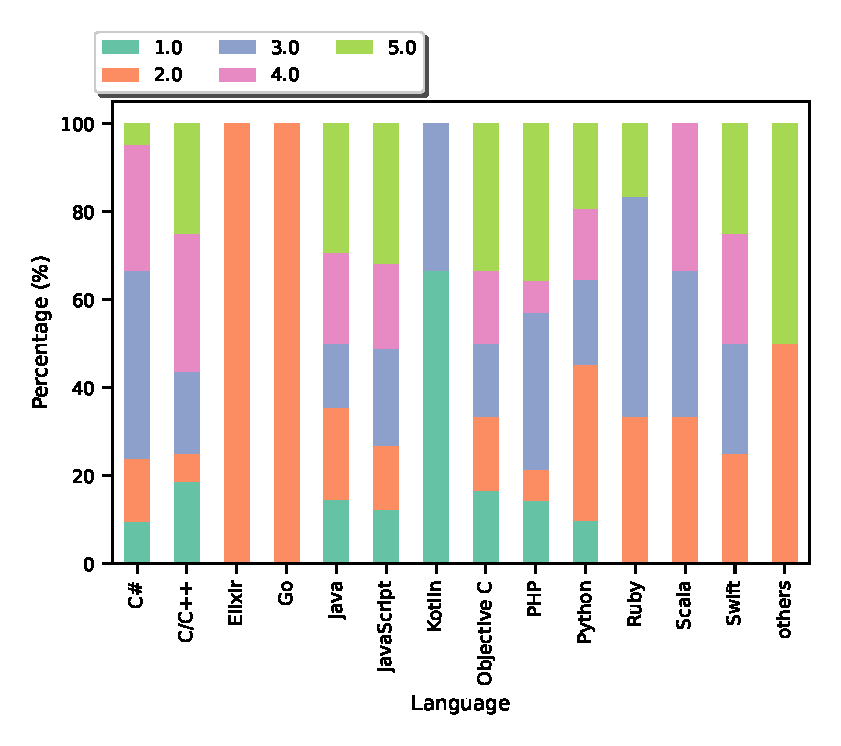
\includegraphics[scale=0.65]{Figures/Language_and_Test_Level}
  \caption{Programming language and automated testing level}
  \label{fig:language and autotest}
\end{figure}
\begin{figure}[h]
\centering
  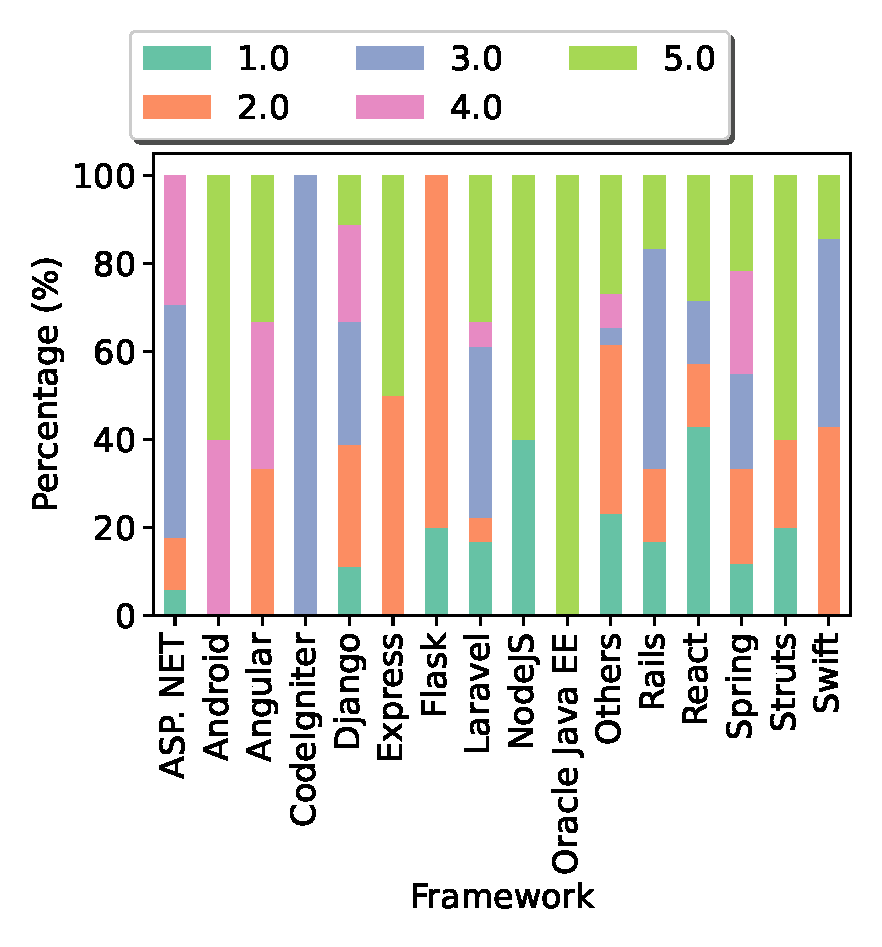
\includegraphics[scale=0.65]{Figures/Framework_and_Test_Level}
  \caption{Framework and automated testing level}
  \label{fig:framework and autotest}
\end{figure}

\begin{figure}[h]
\centering
  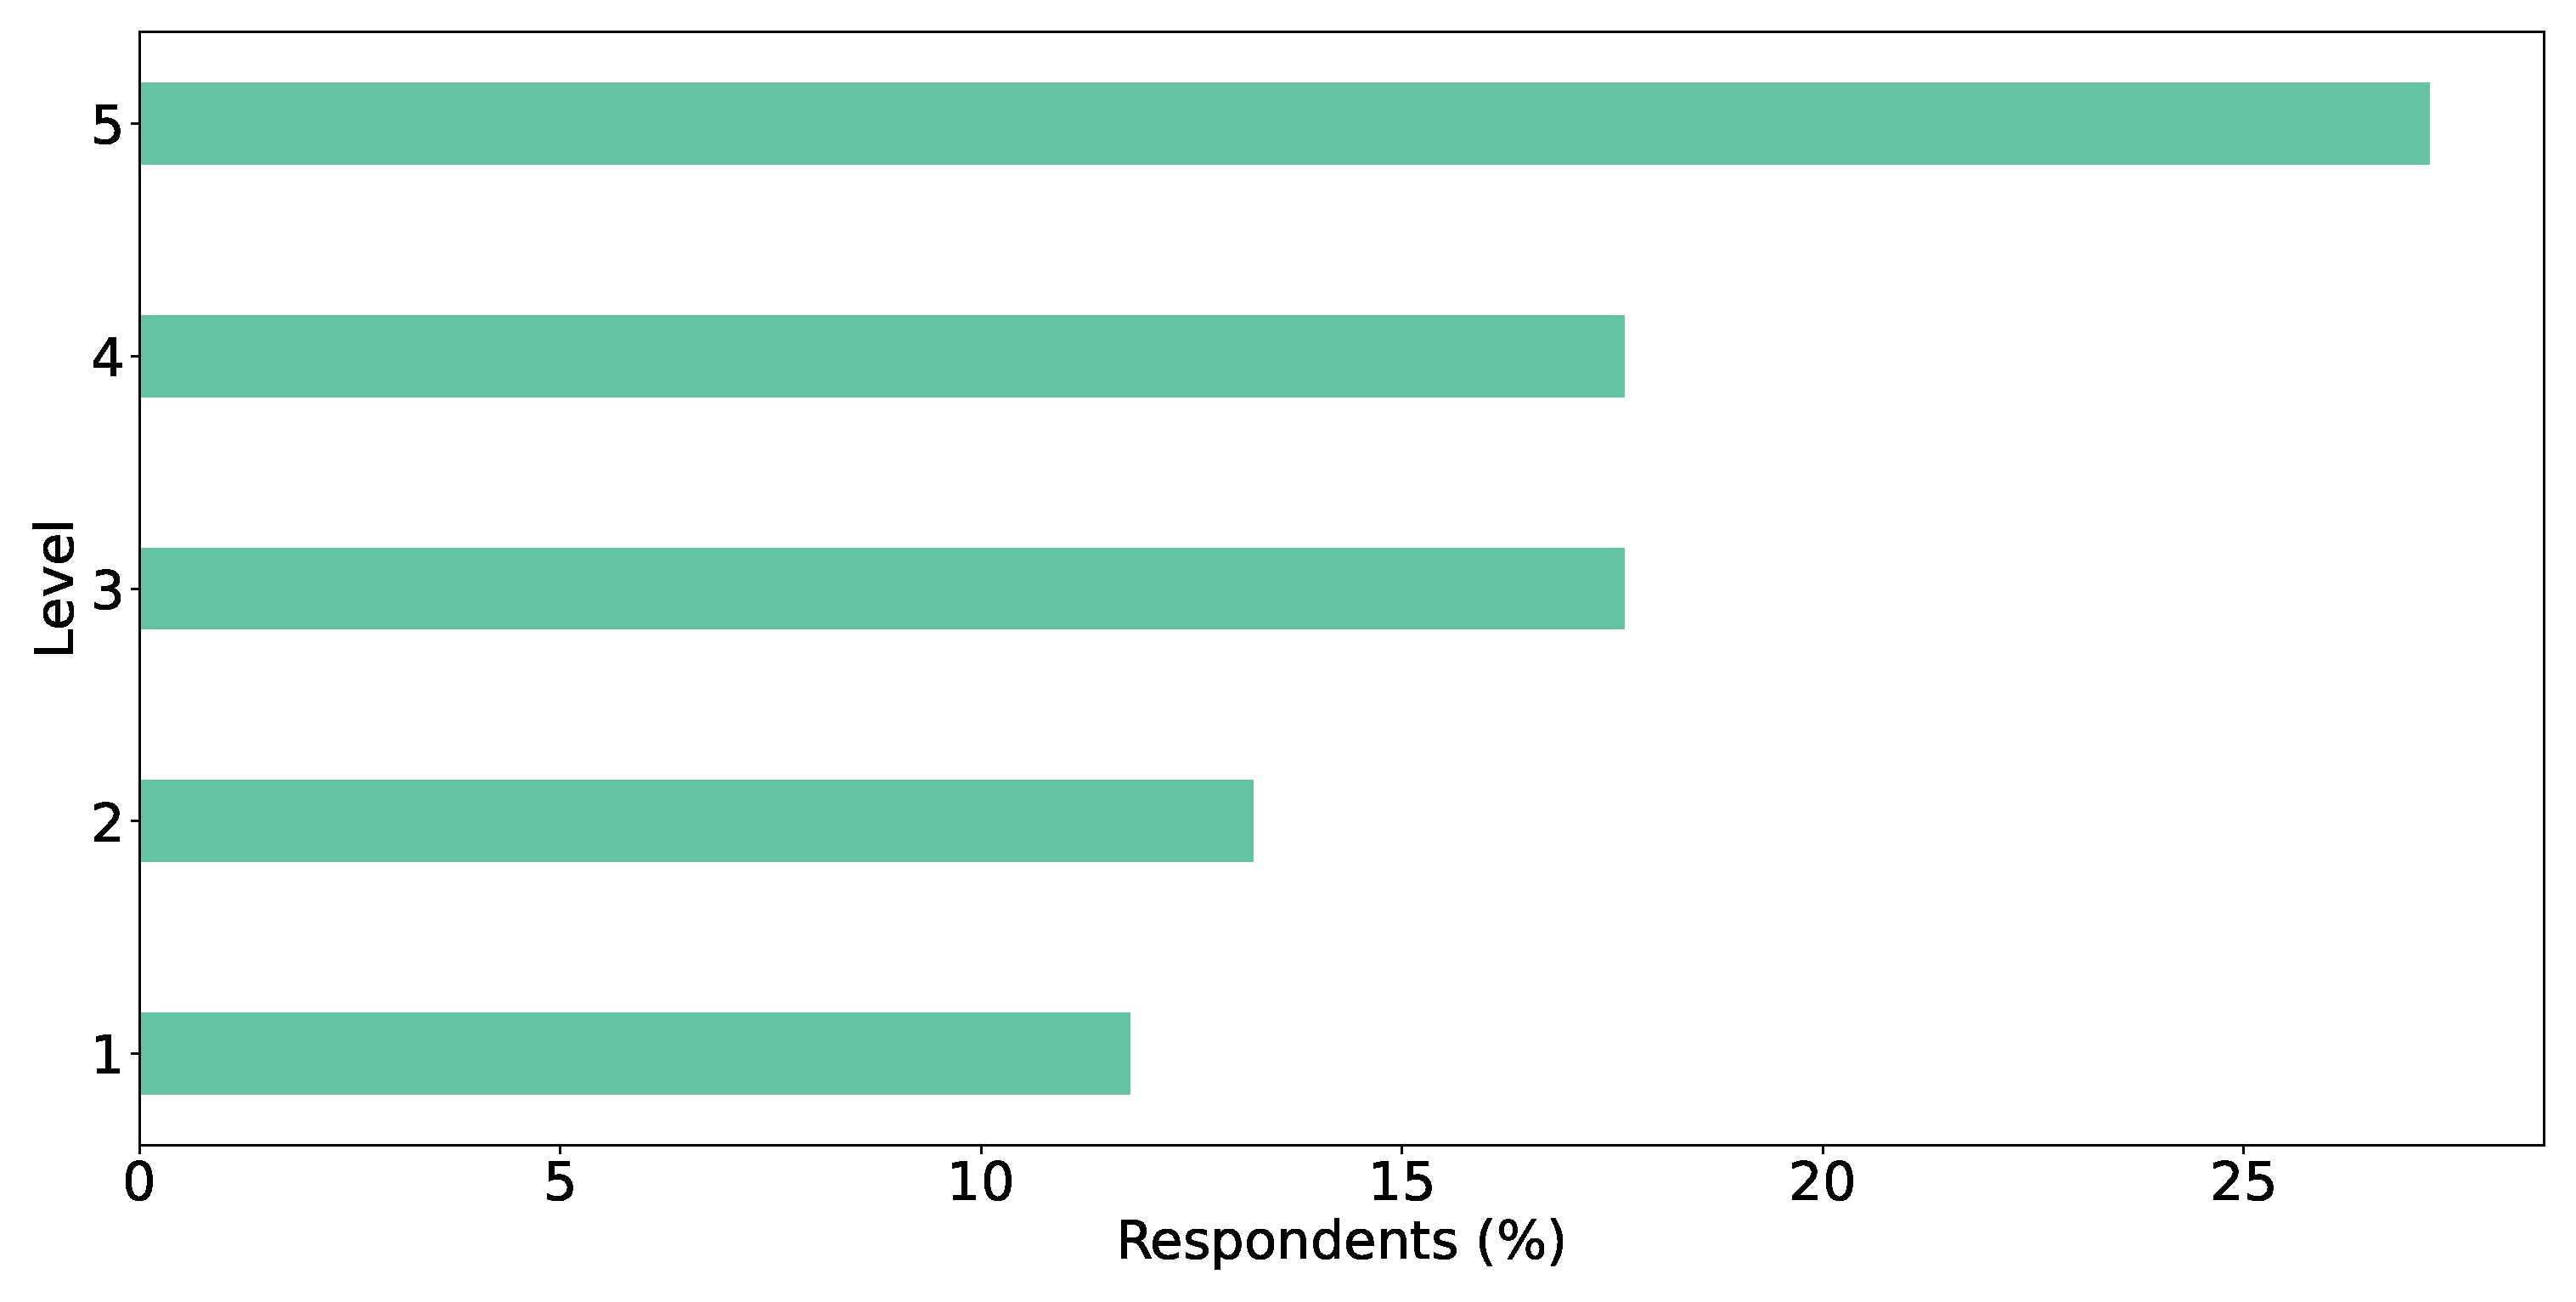
\includegraphics[scale=0.15]{Figures/Respondents_autotest_level}
  \caption{Automated Testing Level}
  \label{fig:autoTest}
\end{figure}

\boxtext{There exists a tendency among most of the Bangladeshi developers not to use automated testing regularly.}
\anindya{Can it be the case that automated testing is done by SQA team, not regular developers?}


\paragraph{Tools Used in Testing and QA}
Q16 asked about the tools used in testing and quality assurance. According to \ref{fig:testingTools}, we see that most of the respondents have used XUnit( eg, JUnit, NUnit) (30\%), selenium (27\%), Jenkins (20\%), others (9\%). These results show that there exists a great demand for testing tools in the software industry of Bangladesh. However, around 38\% of our respondents were not interested to reply to this question that is not surprising because the majority of the respondents (93\% approx.) were working on roles other than SQA engineer as per Table \ref{tab:role}, and they are not supposed to be involved in any testing themselves. \anindya{This may be because many developers are not involved in any sort of testing themselves and our respondents are dominated by developers.} \khalid{added}

\begin{figure}[h]
\centering
  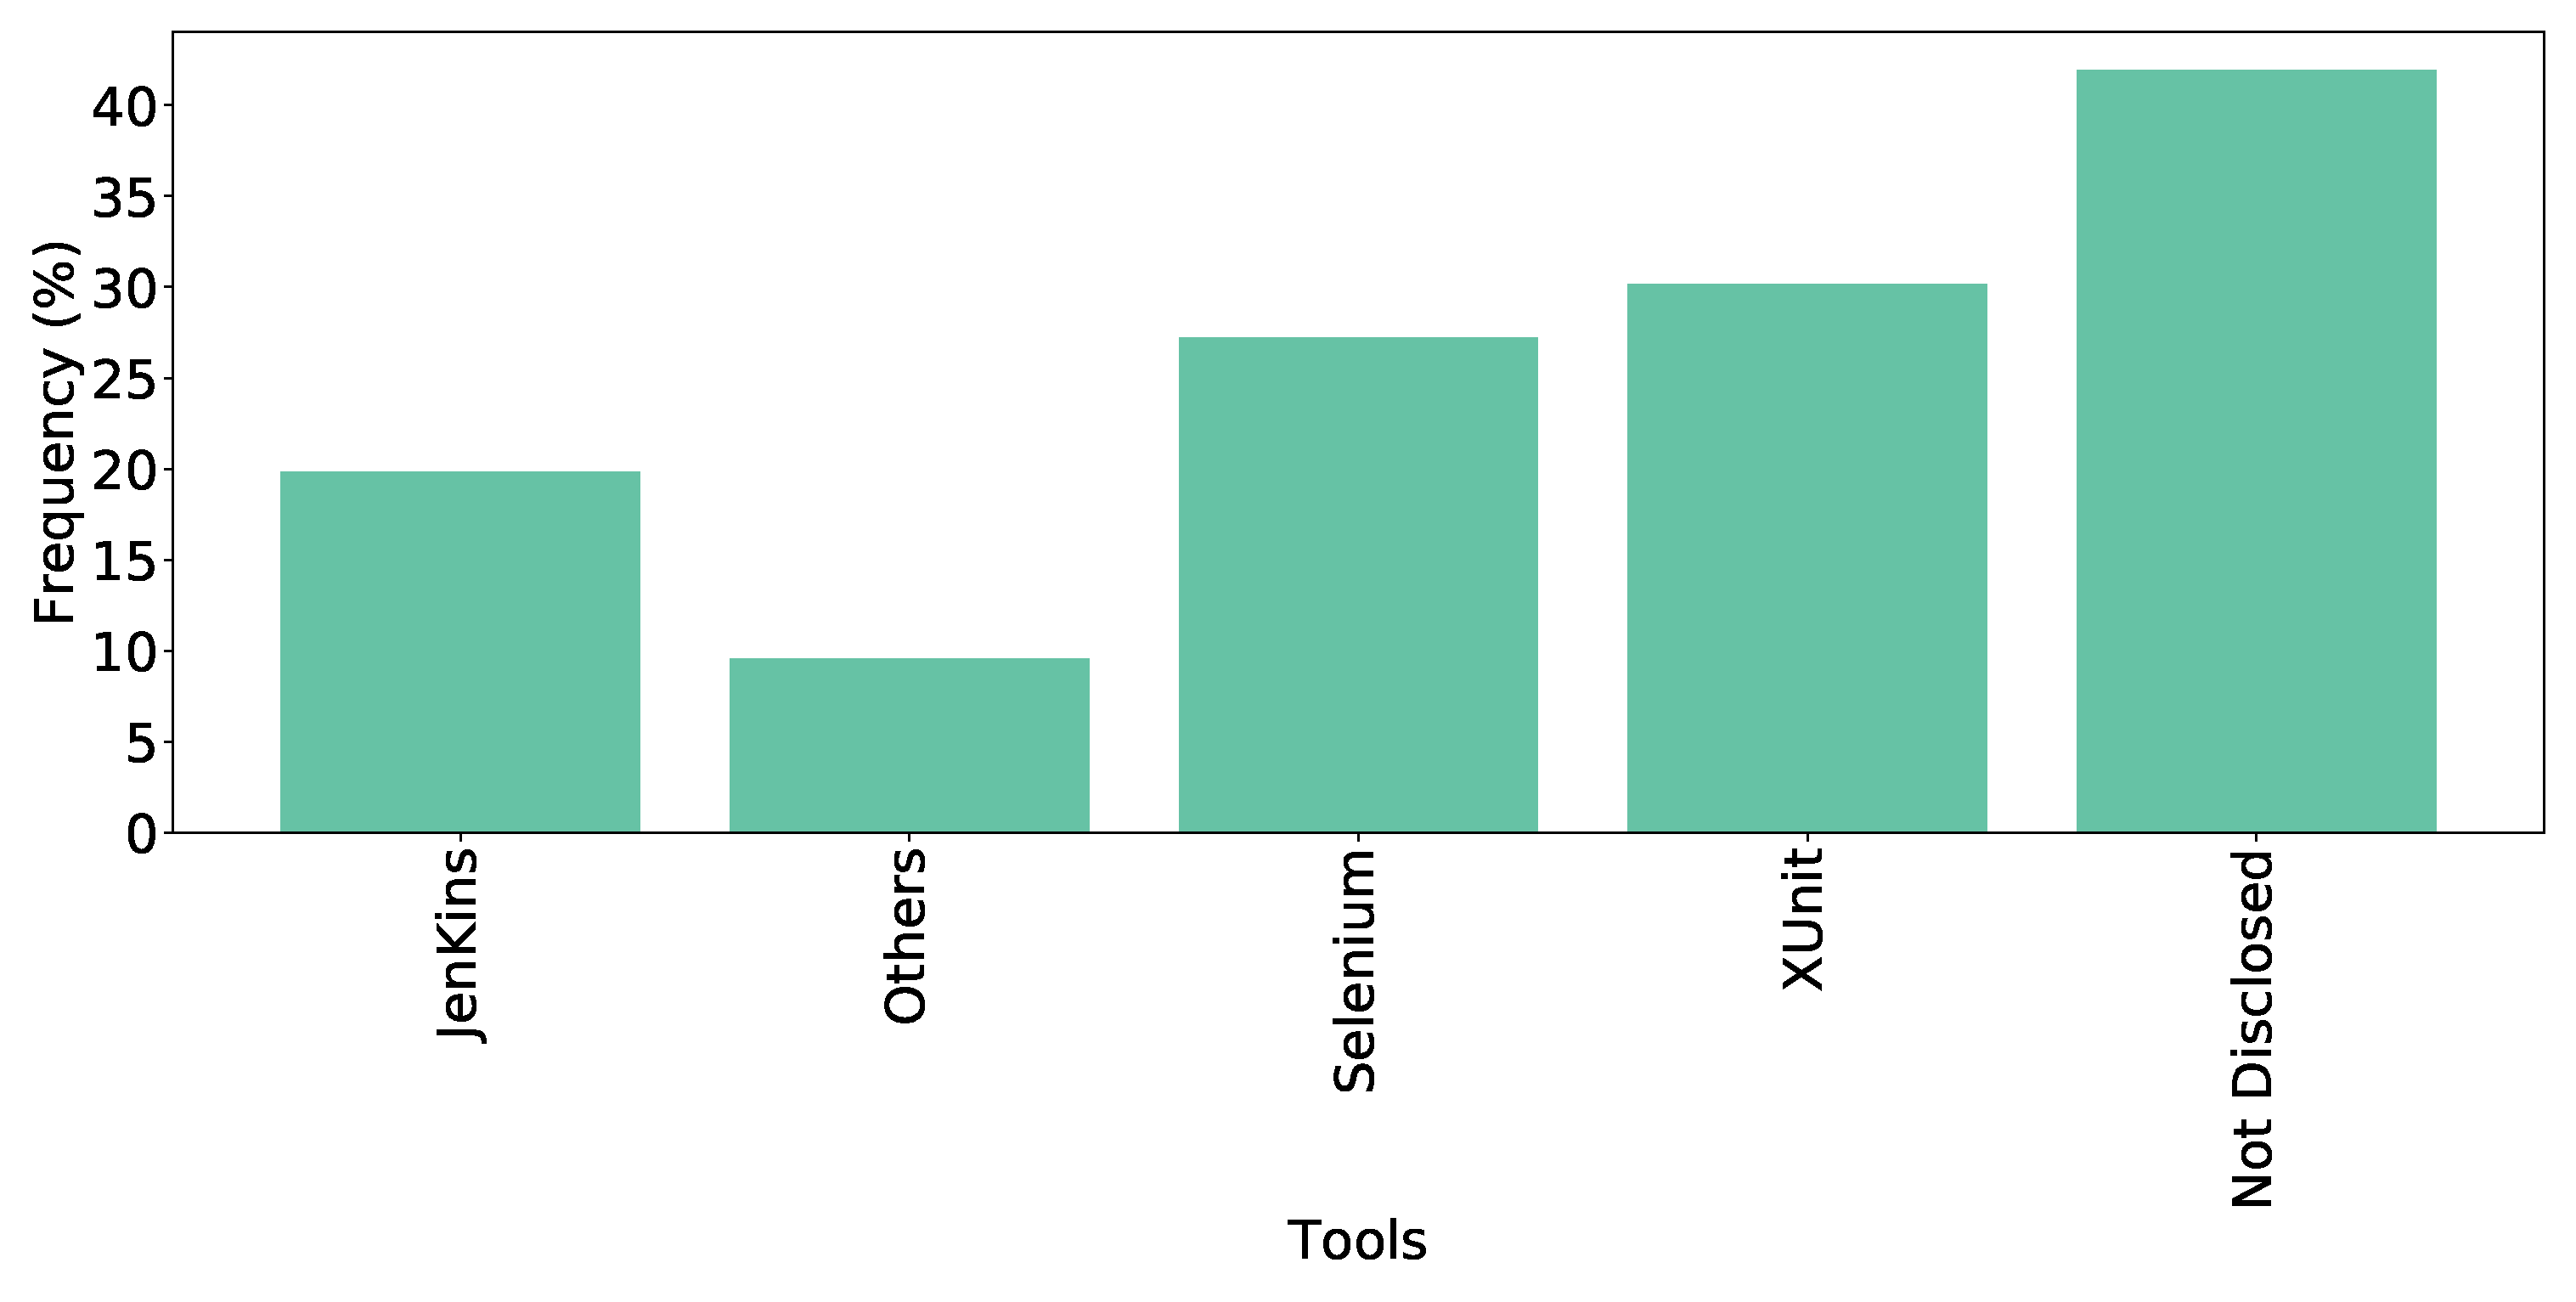
\includegraphics[scale=0.18]{Figures/Respondents_testing_tools}
  \caption{Testing \& QA Tools}
  \label{fig:testingTools}
\end{figure}

\boxtext{There has a large demand of software testing tools in Bangladesh.}


\paragraph{Deployment Tools}
According to \ref{fig:deployTools}, we see that most of the respondents deploy their implemented codes using AWS code-deploy (12\%) and Jenkins (12\%). The other deployment tools are Bamboo (5\%), TeamCity (4\%), Octopus (2\%), etc. Respondents voted none (4\%) as they didn't use any deployment tools and 53\% of the respondents were not interested in this topic. Anyhow, the percentage of the uninterested respondents does not seem unexpected. From Table \ref{tab:role} and \ref{tab:experience}, we can observe that a significant portion of our respondents is developers, and more than half of our respondents are experienced for less than five years respectively. As deployment is related to DevOps, it is quite likely that developers have not enough knowledge or have less interest in deployment. \anindya{Again, this is mostly a dev op related issue and the developers are not likely to respond in this regard.} \khalid{added} The outcome indicates that the usage rate of deployment tools in Bangladesh for continuous integration and continuous deployment is yet to be widespread. We also guessed that the practice of using deployment tools might be done only by senior practitioners. However, the hypothesis is not statistically significant ($p=0.37$).

\begin{figure}[h]
\centering
  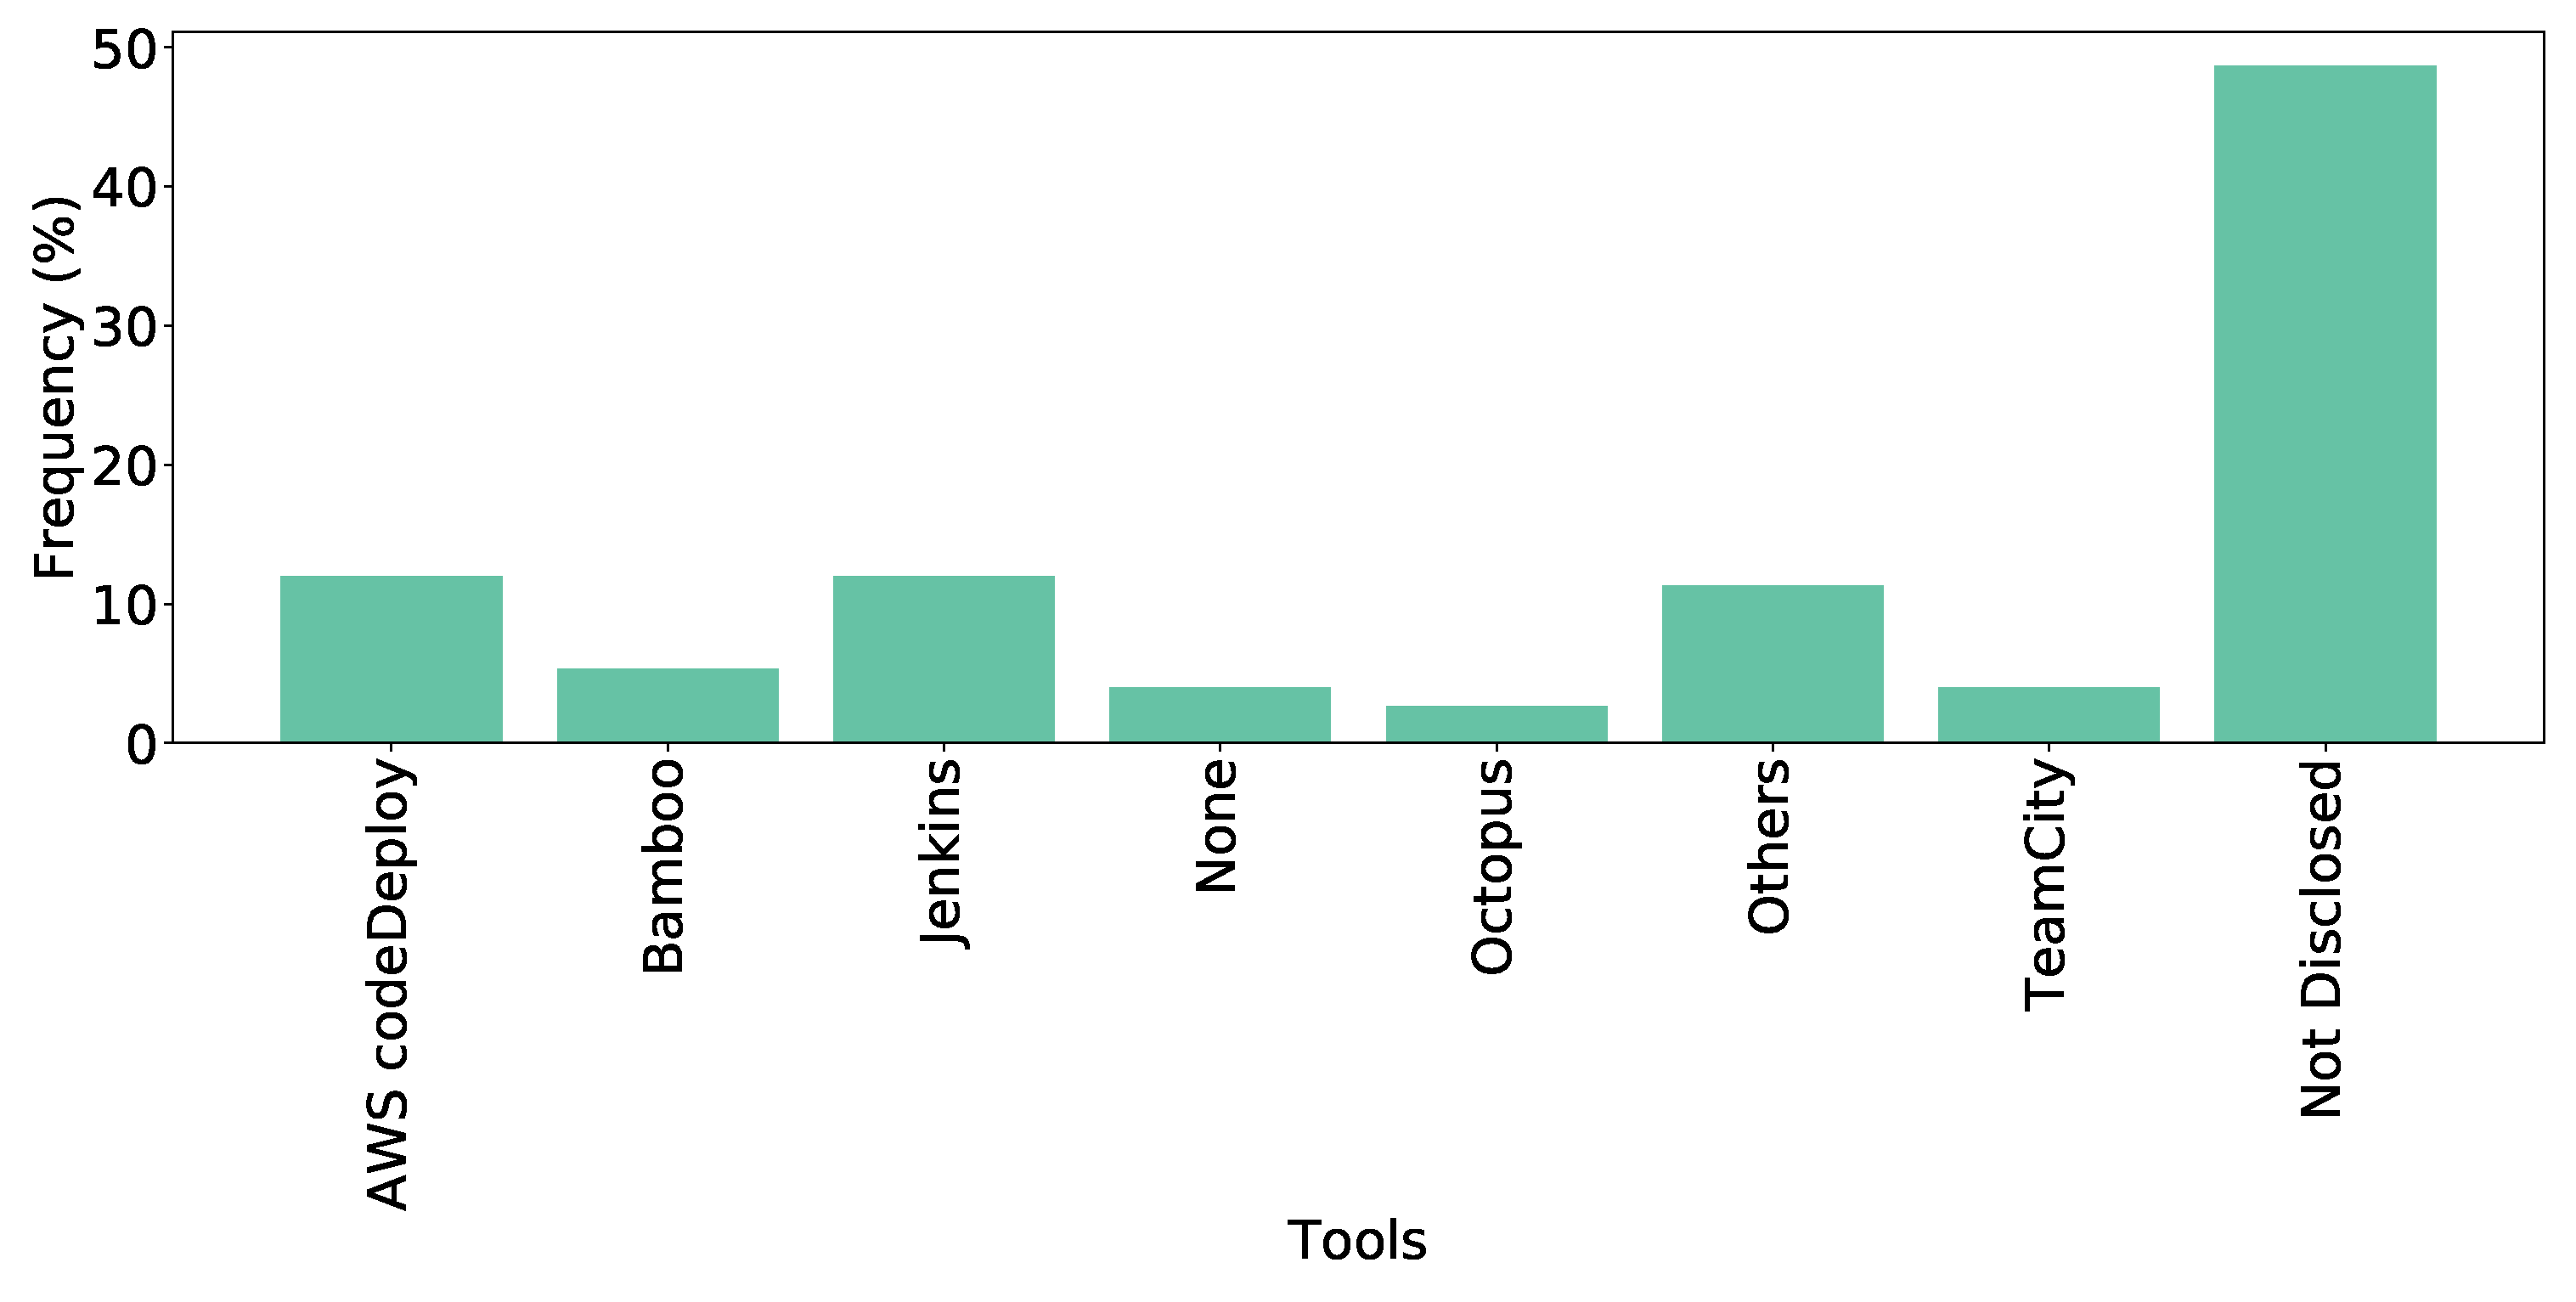
\includegraphics[scale=0.18]{Figures/Respondents_deployment_tools}
  \caption{Deployment Tools}
  \label{fig:deployTools}
\end{figure}


\paragraph{Version Control}
% \hfill\\

Respondents were allowed to select more than one option. As shown in Figure \ref{fig:versionControl}, Git (78\%) and Bit-Bucket (29\%) are mostly-used version control systems in the software industry. Besides these, Subversion (SVN) (5\%) and others (4\%) are used.  The 2018 Stack overflow survey\cite{StackoverflowSurvey2018} reports that the most popular version control system is Git (87.2\% developer uses Git) and the second most popular is SVN (16.1\% developer uses SVN). However, in our survey, we found a slightly different result, the most popular version control system is Git and the second most popular is Bit-bucket. This might be related to the declining popularity of SVN over the years. From the Stack overflow survey over the range 2017-2018, it is clear that SVN is losing popularity to Git. Nowadays, SVN is mainly used for versioning legacy projects. As the SE industry of Bangladesh is relatively young, this discrepancy observed is not surprising.
\anindya{It looks nice that you compared with external relevant source like SO. Is it possible to do it for other RQs? Also, you may mention such deviations from other trends in Introduction.} \khalid{added in `methodologies', `tech platform', `test practices'} \partha{added in `os', `languages', `framework'}
\begin{figure}[h]
\centering
  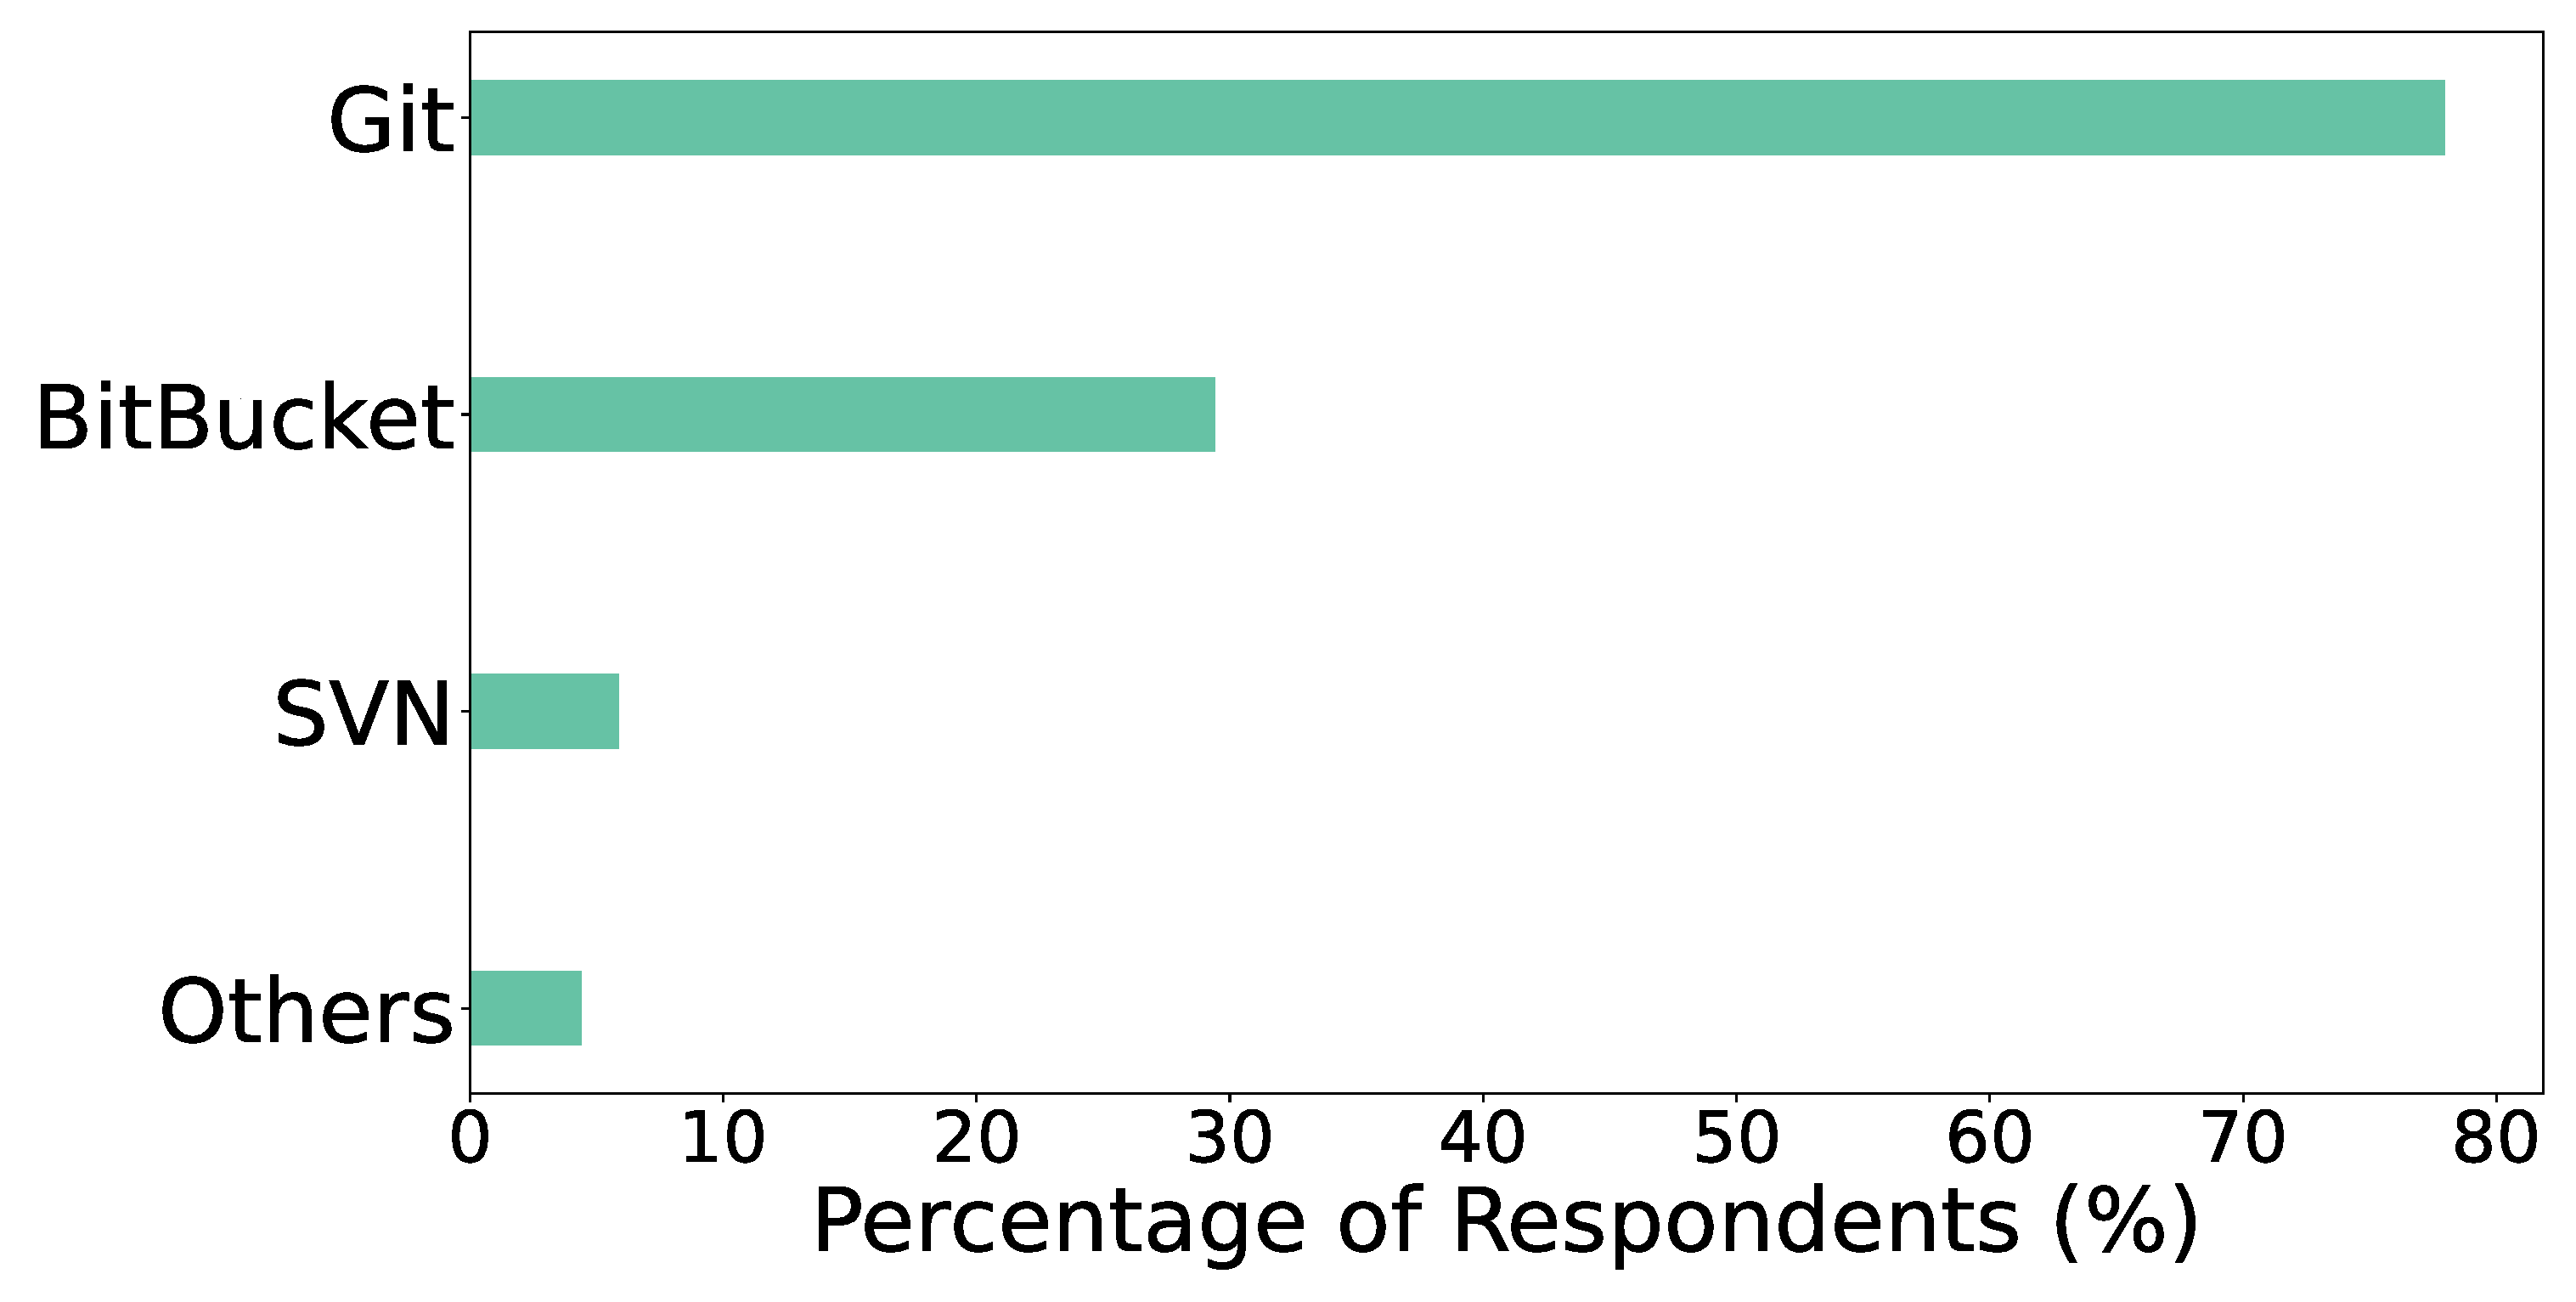
\includegraphics[scale=0.16]{Figures/Respondents_version_control}
  \caption{Version Control}
  \label{fig:versionControl}
\end{figure}

\subsubsection{Performance and security measures used (D4)}
\label{security_performance}
Security and performance are two of the most important non-functional requirements for any software product. 
We asked three open-ended questions with regards to the enforcement of security and performance-related features in software products in Bangladesh:
How do you ensure performance, scalability (Q21, Q22) and security (Q23) in your software products?

% To identify general practices among the Bangladeshi software companies regarding software products' security and performance, we have included two open-ended questions in the survey. This particular question covers how a company secures its developed products from security threats and maintain performance after deployment. However, the scalability of software directly impacts its performance\citep{Liu2009,Bondi2000}. Hence, we will cover the following points here:
% \begin{itemize}
%     \item Security
%     \item Performance
%     \item Scalability
% \end{itemize}


%\label{Security}

\begin{figure}[h]
\centering
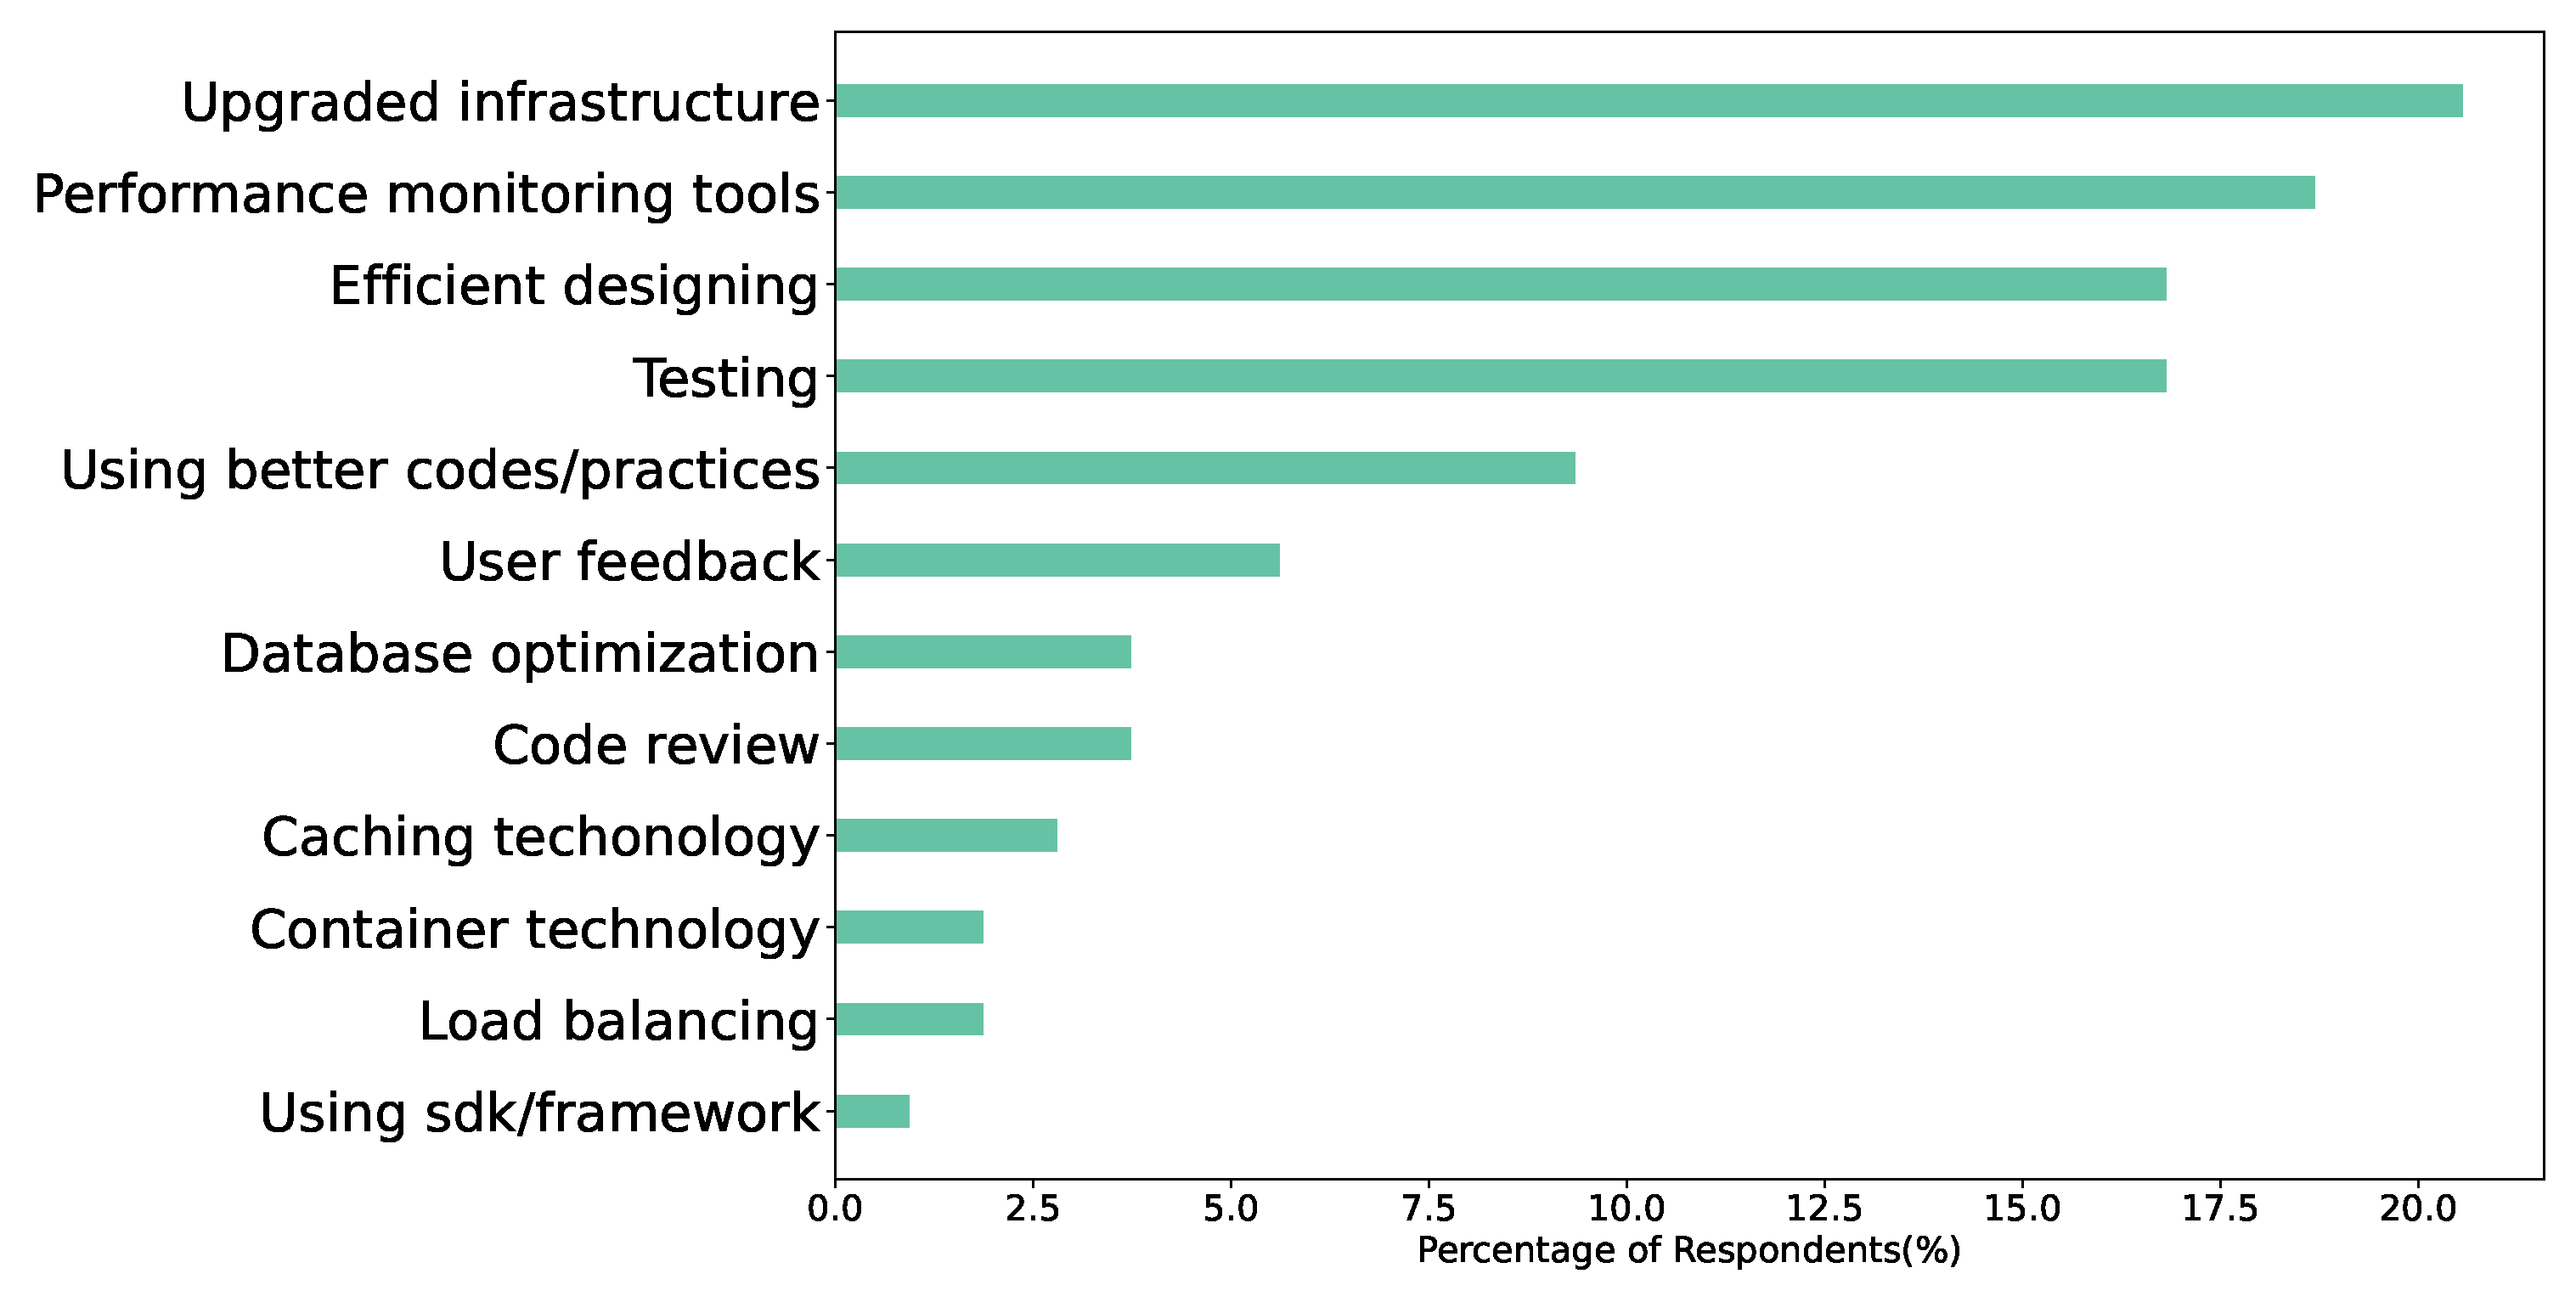
\includegraphics[scale=0.22]{Figures/PerformanceScalability.eps} 
\caption{Measures to ensure performance \& scalability of products}
\label{fig:Measures to ensure performance and scalability}
\end{figure}
\nd\bf{$\bullet$ Performance (Q21, Q22).} Software performance indicates how efficient the software is in terms of response time and resource consumption. 
We find nine types of performance measures that are practised in software products developed in Bangladesh (see Figure \ref{fig:Measures to ensure performance and scalability}).  
The twelve types are divided into four categories: 
\begin{inparaenum}
Use of \item tools and frameworks (46.72\%),
\item design principles/best practices (26.17\%),
\item testing (16.82\%), and
\item review and feedback (9.35\%).
\item database optimization (3.74\%)
\end{inparaenum} 

\begin{inparaenum}[(1)]
\item \ib{Exploitation of tools and frameworks.} Six out of twelve types belong to this category.
\begin{inparaenum}%[label=(\alph*)]
    \item \it{Tools}: Around 18.69\% respondents use tools and metrics to
    measure performance:  \emt{take help of different performance monitoring tools and dashboard, analyzed data, measure time and memory efficiency of process}($S_{35}$)
    \item \it{Infrastructure}: Around 20.56\% of respondents use upgraded
    infrastructure to ensure performance like cloud
    hosting (e.g., Amazon AWS), a high-end server, and new technologies.
    %\emt{Amazon Hosting and Quality Software}{85}
    \item \it{Caching}: Around 2.8\% respondents implemented caching to maintain
    software performance.
    % \emt{... Good Caching}{29}
    \item \it{Container Technology}: Containers enable users to scale their system without any dependency on the underlying OS. About 1.87\% of our respondents use container technologies to ensure their products scalability and performance.
    \item \it{Using SDK/framework}: About 0.93\% of respondents depend on the framework to maintain software performance and scalability.
    \item \it{Load Balancing}: Around 1.87\% respondents use load
    balancing as a measure to maintain performance:
    \emt{Optimizing number of HTTP requests, Asynchronous programming, Caching, CDN, Load Balancing, nginx, varnish, compression of data, 
    Continuous monitoring, Load testing, stress testing}($S_{42}$)
\end{inparaenum}
 
\item \ib{Use of design principles/best practices.}  Around 26.17\% respondents try to ensure software performance right from the design phase as follows.
\begin{inparaenum}%[label=(\alph*)]
    \item \it{Using better codes/practices}: Around 9.35\% respondents ensure performance by
    implementing industry-standard best practices like compression
    technology, enforcing design patterns, and refactoring.
    %\emt{Implementation time carefulness and maintaining a well developed coding standard}{40}
    \item \it{Efficient designing}: Around 16.82\% of respondents emphasize on
    performance-aware architecture design.
    %\emt{By careful designing}{24}
\end{inparaenum}

\item \ib{Use of testing.} Around 16.82\% respondents rely on the software testing strategy to ensure performance like load testing and stress testing.

\item \ib{Use of review and feedback.} Around 9.35\% of our respondents use user feedback (e.g., continuous feedback from QA team $S_{65}$) 
and code review to improve product performance. According to $S_{15}$: \emt{The code quality is assessed by the different team members during code review, followed by designing new ways to solve issues in the product that are time-intensive.}

\item \ib{Database Optimization.} Around 3.74\% of our respondents use database optimization to ensure performance and scalability. Database optimization includes sharding, clustering, indexing, and scaling. According to $S_{85}$: \emt{Besides scaling horizontally, database scaling is performed by partitioning tables, along with multi-threaded implementations}

\end{inparaenum}


\begin{figure}[h]
\centering
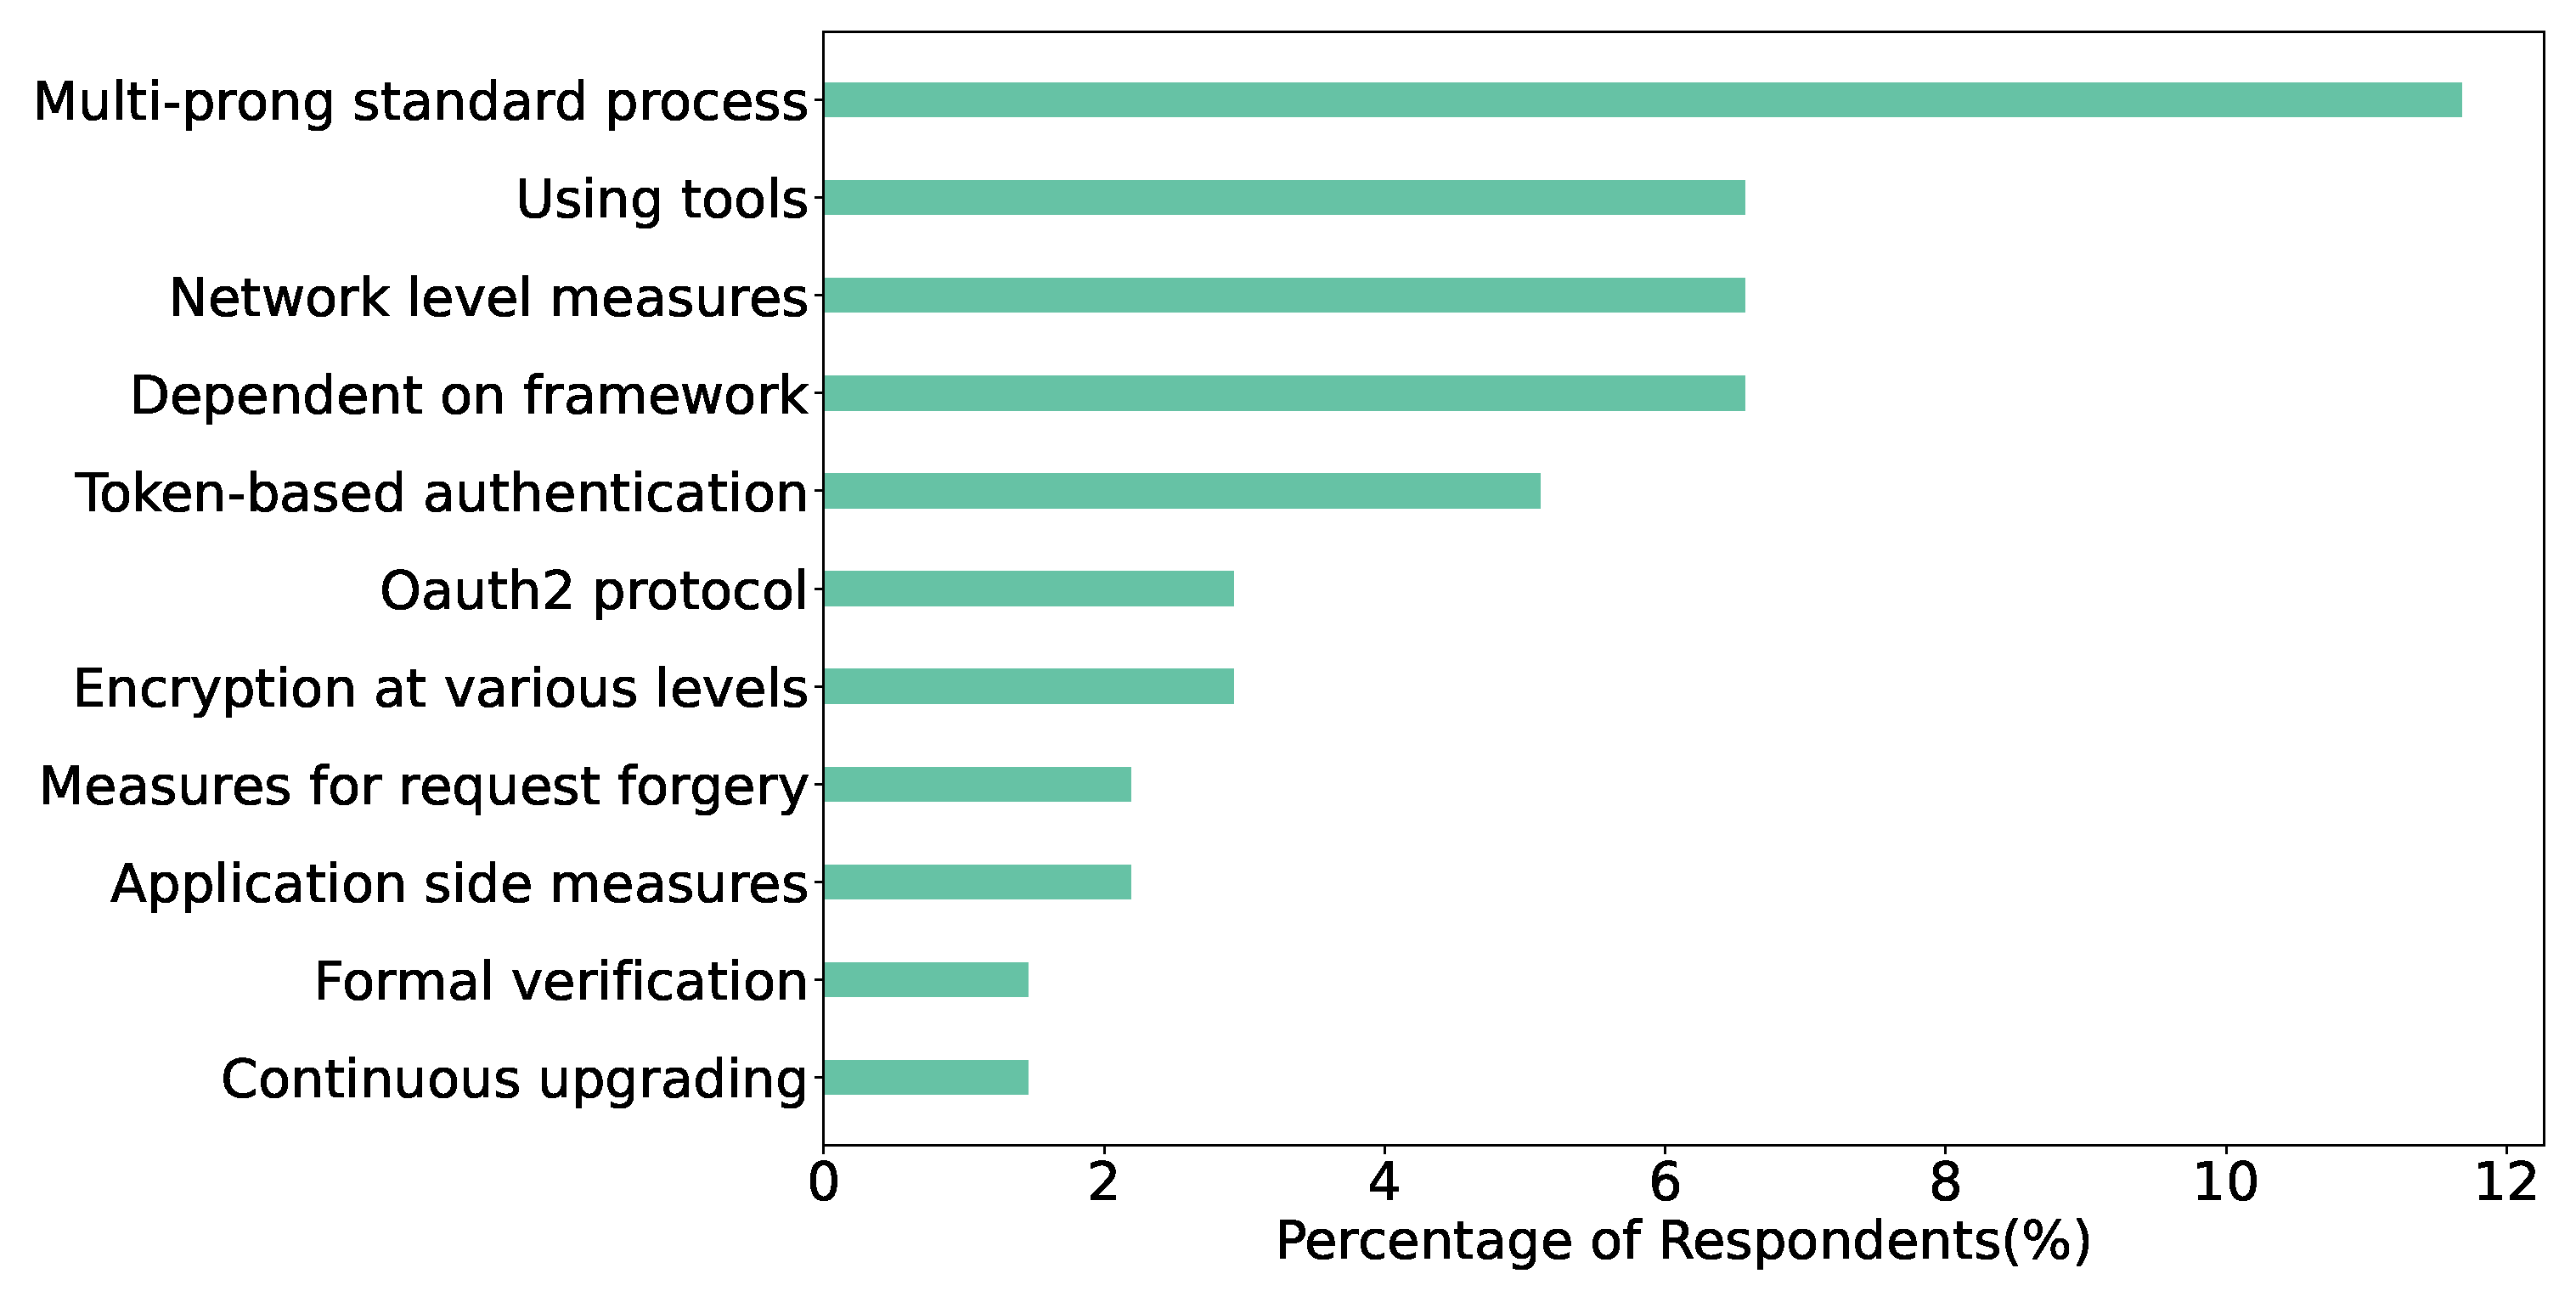
\includegraphics[scale=0.22]{Figures/Security.eps} 
\caption{Measures to ensure security of products}
\label{fig:Measures to ensure security}
\end{figure}
\nd\bf{$\bullet$ Security (Q23):} Our open coding of the survey responses reveals 11  
labels (see Figure \ref{fig:Measures to ensure security}). The 11 labels are are divided into three main categories of security-related development practices: 
\begin{inparaenum}
\item Measures related to authentication and authorization (64.82\%),
\item Exploitation of tools and techniques to ensure security in products (53.71\%), and 
\item Use of encryption technologies for data (7.41\%).
\end{inparaenum} We discuss the categories below.  


\begin{inparaenum}[(1)]
\item \ib{Measures related to authentication and authorization.} Six out of the 11 labels belong to this category. 
\begin{inparaenum}
\item \it{Multi-prong Standard Process}. About 29.6\% of the respondents
reported that they practice various security standards and protocol to
ensure security (e.g., ISO/IEC 27001, PA DSS).
\item \it{Token-based authentication.} About 13\% respondents reported to 
have implemented a token-based authentication system, which 
allows users to enter their username and password to obtain a token for authentication and authorization.
\item \it{OAuth 2.0} : Around 7.4\%) respondents use the OAuth 2.0
protocol as the primary way of maintaining security. OAuth 2.0 is the industry-standard protocol for
authorization. OAuth 2.0 focuses on client developer simplicity while providing
specific authorization flows for web applications, desktop applications, mobile
phones, and living room devices. %, e.g., \emt{OAuth 2.0,
\item \it{Application-side measures}: Around 5.6\% of respondents 
implement security measures at the application level like encryption of application data at the client-side, use of https while
pulling data from a server, secured architecture, etc.
\item \it{Measures for request forgery}: Around 5.6\% respondents implemented security measures against
Cross-site request forgery (e.g., attacks like
cross-origin resource sharing (CORS), cross-site request forgery (CSRF) or
one-click attack or XSRF). Security testing is paramount for this: \emt{Security testings
like: SQL injection, cross-site scripting, CSRF, API security, use of https, 
detecting malicious/suspicious HTTP requests and auto-blocking} (Respondent ID $S_{42}$)
    \item \it{Formal Verification}: Around 3.7\% respondents ensured the practice of formal code review to enforce security practices: \emt{There are some basic
    guidelines that we must follow and while code review this needs to be an
    absolute part that needs to be checked before the code gets merged} ($S_{112}$)
    \end{inparaenum}

\item \ib{Exploitation of tools and techniques to ensure security in products.} Four out of the 11 labels belong to this category. 
\begin{inparaenum}
  \item \it{Dependent on Framework}: Around 16.7\% 
  respondents depend on the underlying framework for security like Spring, HDIV, and Laravel. 
  \emt{https, popular framework which already prevents some type of attacks. rest of the things on case-by-case basis)}($S_{79}$)
  \item \it{Use of tools}: Respondents use various open-source/paid tools for
  scanning and testing like OWASP and penetration testing tools.
  %\emt{use encryption at different level of software (server, network, transmission layer, database and software layer.)}{35}
  \item \it{Network level Measures}: Network-level measures include
  IP-white-listing, port-blocking, VPN, and the use of HTTPS in software.
  16.7\% of respondents use at least one of the mentioned strategies to ensure
  security.
  %\emt{network blocking and common security measures}{2}
  \item \it{Continuous Upgrade}: Around 1.5\% 
  respondents reported that they arrange frequent hackathons, workshops, and
  security audits: \emt{We run security audit of our office environment. We also conduct security session per 6 months to introduce latest trend in threats and what we can do to avoid it}($S_{57}$)
\end{inparaenum}

\item \ib{Use of encryption technologies for data}. Around 7.4\% respondents use encryption at
the different levels of software architecture such as network, data, and
transmission.
\emt{use encryption at different level of software (server, network, transmission layer, database and software layer.)}($S_{35}$)
\end{inparaenum}
% 
% Authentication and authorization based security are the most prominent practices in the software industry of Bangladesh. The other techniques used widely include framework, platform, tools, and encryption. Under these categories, several measures are usually followed. The security measures of the Bangladesh SE industry is presented in Figure \ref{fig:Measures to ensure security}. The measures of each category are discussed below.
% 
% Measures under the \emph{authentication and authorization} category is practised by 53.71\% respondents to ensure security. The measures are 
% \begin{enumerate}[label=(\alph*)]
% 
%     \item \textbf{Multi-prong Standard Process}: About 29.63\% of the respondents reported that they practice various security standards and protocol to ensure security. The standard includes ISO/IEC 27001 and PA DSS.
%     \surveyquote{Multi Prong Standard Processes and Products}{110}
%     
%     \item \textbf{Token-based authentication}: A token-based authentication system allows users to enter their username and password to obtain a token, which allows them to fetch a specific resource without using their username and password. Once their token has been obtained, the user can offer the token, which offers access to a specific resource for a time period to the remote site. 12.96\% of people expressed its eligibility.
%     \surveyquote{Token based authentication for all of my rest service}{80}
%     
%     \item \textbf{OAuth 2.0} : OAuth 2.0 is the industry-standard protocol for authorization. OAuth 2.0 focuses on client developer simplicity while providing specific authorization flows for web applications, desktop applications, mobile phones, and living room devices. Many (7.41\%) respondents use the OAuth 2.0 protocol as the primary way of maintaining security.
%     \surveyquote{OAuth 2.0, JWT, Token Based Authentication, CORS Filter, XSRF}{127}
%     
%     \item \textbf{Application-side measures}: 5.56\% of respondents responded that they would implement security measures at the application level. This measure includes encryption of application data at the client-side, use of https while pulling data from a server, secured architecture, etc.
%     \surveyquote{At application level, could not achieve others yet}{72}
%     
%     \item \textbf{Measures for request forgery}: Cross-site forgery attacks include cross-origin resource sharing (CORS), cross-site request forgery (CSRF) or one-click attack or XSRF. 5.56\% of respondents implemented measures against  Cross-site request forgery to ensure security.
%     \surveyquote{Security testings like: SQL injection, cross-site scripting, CSRF, API security, use of https,  detecting malicious/suspicious HTTP requests and auto-blocking}{42}
%     
%     \item \textbf{Formal Verification}: A code-level review can mitigate security threats. 3.7\% respondents ensured the practice of formal code review.
%     \surveyquote{There are some basic guidelines that we must follow and while code review this needs to be an absolute part that needs to be checked before the code gets merged}{112}
%     
% \end{enumerate}

% 53.71\% respondents exploit several technologies, tools, and platforms to ensure the security of their products. Measures under the \emph{framework/platform/tools} can be categorized as follows:
% 
% \begin{enumerate}[label=(\alph*)]
%   \item \textbf{Dependent on Framework}: The common frameworks provide basic to intermediate level security measures in the application. 16.67\% of respondents depend on the framework for security. The frameworks include popular ones such as Spring and HDIV. We have found that respondents using Spring and Laravel framework mostly reported depending on the framework for security. However, the observation is not statistically significant.
%   \surveyquote{https, popular framework which already prevents some type of attacks. rest of the things on case-by-case basis)}{79}
%   
%   \item \textbf{Use of tools}: Respondents use various open-source/paid tools for scanning and testing. These tools help to find security threats in an existing system. The tools include OWASP provided and penetration testing tools.
%   \surveyquote{use encryption at different level of software (server, network, transmission layer, database and software layer.)}{35}
%   
%   \item \textbf{Network level Measures}: Network-level measures include IP-white-listing, port-blocking, VPN, and the use of HTTPS in software. 16.67\% of respondents use at least one of the mentioned strategies to ensure security.
%   \surveyquote{network blocking and common security measures}{2}
% 
%   \item \textbf{Continuous Upgrade}: As security threats evolve continuously, the applications need continuous up-gradation at a frequent interval. 1.46\% of respondents said that they would arrange frequent hackathons, workshops, and security audits to address the continuously evolving security threats.
%   \surveyquote{We run security audit of our office environment. We also conduct security session per 6 months to introduce latest trend in threats and what we can do to avoid it}{57}
% \end{enumerate}

%\boxtext{Security testing and the use of security standards are prevalent in the Bangladesh SE industry.}


% To maintain security of software product SE industry of Bangladesh is mainly dependent on standard process which includes cloud based security, third party software, OS hardening followed by uses of security tools, network level measures and framework security. As found by Harrison et al.\citep{Harrison2010} network level measures are the first choice in ensuring security of software product which matches with our findings. Srinivasan et al.\citep{Srinivasan2017} listed top 10 web framework in terms of security testing where Spring framework achieved 7\textsuperscript{th} position. From figure ~\ref{fig:frameworks} we have seen that most of our respondents use Spring framework for software development. This might be the reason that a lot number of respondents dependent on framework for ensuring security.


% 
% Software performance indicates how efficient the software is in terms of response time and resource consumption. Our open coding of the survey responses reveals four main categories of performance-related development practices: 
% The measures are presented in Figure \ref{fig:Measures to ensure performance}.

% 
%  The use of framework/tools/platform to ensure software performance is a dominant (58.18\%) practice in the SE industry. Respondents in our survey reported multiple measures under these categories.
%  The measures belonging to \emph{framework/tools/platform} category are as follows:
% 
% \begin{enumerate}[label=(\alph*)]
%     \item \textbf{Performance Monitoring Tools}: There are various automated performance monitoring tools from which we can measure the overall and component-wise performance. 36.36\% of respondents use these tools to measure performance. Respondents use several performance metrics such as error/crash rate, response time, uptime, etc.
%     \surveyquote{take help of different performance monitoring tools and dashboard, analyzed data, measure time and memory efficiency of process}{35}
%     
%     \item \textbf{Upgraded Infrastructure}: 12.73\% of respondents use upgraded infrastructure to ensure performance. This infrastructure includes cloud hosting, a high-end server, and new technologies.
%     \surveyquote{Amazon Hosting and Quality Software}{85}
%     
%     \item \textbf{Caching Technology}: Caching mechanism improves performance by reducing response time. 5.45\% of respondents rely on caching to maintain software performance.
%     \surveyquote{... Good Caching}{29}
%     
%     \item \textbf{Load Balancing}: Load balancing can improve the system performance by ensuring an equal load to all servers. 3.64\% of respondents use load balancing as a measure to maintain performance.
%     \surveyquote{Optimizing number of HTTP requests, Asynchronous programming, Caching, CDN, Load Balancing, nginx, varnish, compression of data, Continuous monitoring, Load testing, stress testing}{42}
% 
% \end{enumerate}
% 
% 
% 32.73\% of respondents try to ensure software performance right from the design phase. Measures of this category are as follows:
% 
% \begin{enumerate}[label=(\alph*)]
% 
%     \item \textbf{Using better codes/practices}: Industry-standard best practices can improve system performance. 18.18\% respondents ensure performance by implementing best practices. The best practices include compression technology, enforcing design patterns, and refactoring.
%     \surveyquote{Implementation time carefulness and maintaining a well developed coding standard}{40}
%     
%     \item \textbf{Efficient designing}: Software performance is dependent on the architecture of the system. 14.55\% of respondents emphasize on performance-aware design to ensure performance.
%     \surveyquote{By careful designing}{24}
% 
% \end{enumerate}
% 
% 21.82\% of respondents of our survey relies on the software testing strategy to ensure performance. Performance testing includes load testing and stress testing.\anindya{Integration testing is not performance testing.}\partha{updated}
%  \surveyquote{By rigorous testing and checking performance testing}{17}
%  
%  Peer code review, user and tester feedback can be a good strategy to ensure performance. 18.18\% of our respondents use measures from this category to ensure performance. Measures under this category are:
%  
%  \begin{enumerate}[label=(\alph*)]
%  
%      \item \textbf{User Feedback}: It is a great source of performance measure. Taking time to time feedback from the clients helps a company realize how their products are performing. Many (10.91\%) respondents have highly recommended it.
%     \surveyquote{Continuous feedback from clients and QA team}{65}
%     
%     \item \textbf{Code Review}: About 7.27\% people have said that a proper and attentive code review can reduce the codes' faults and, therefore, enhance the performance of a software.
%     \surveyquote{The code quality is assessed by the different team members during code review, followed by designing new ways to solve issues in the product that are time-intensive.}{15}
%  
%  \end{enumerate}
%\boxtext{For performance, the SE industry in Bangladesh is largely dependent on monitoring tools and software testing.}


% \paragraph{Scalability}
% \label{Scalability}
% \begin{figure}[h]
% \centering
% 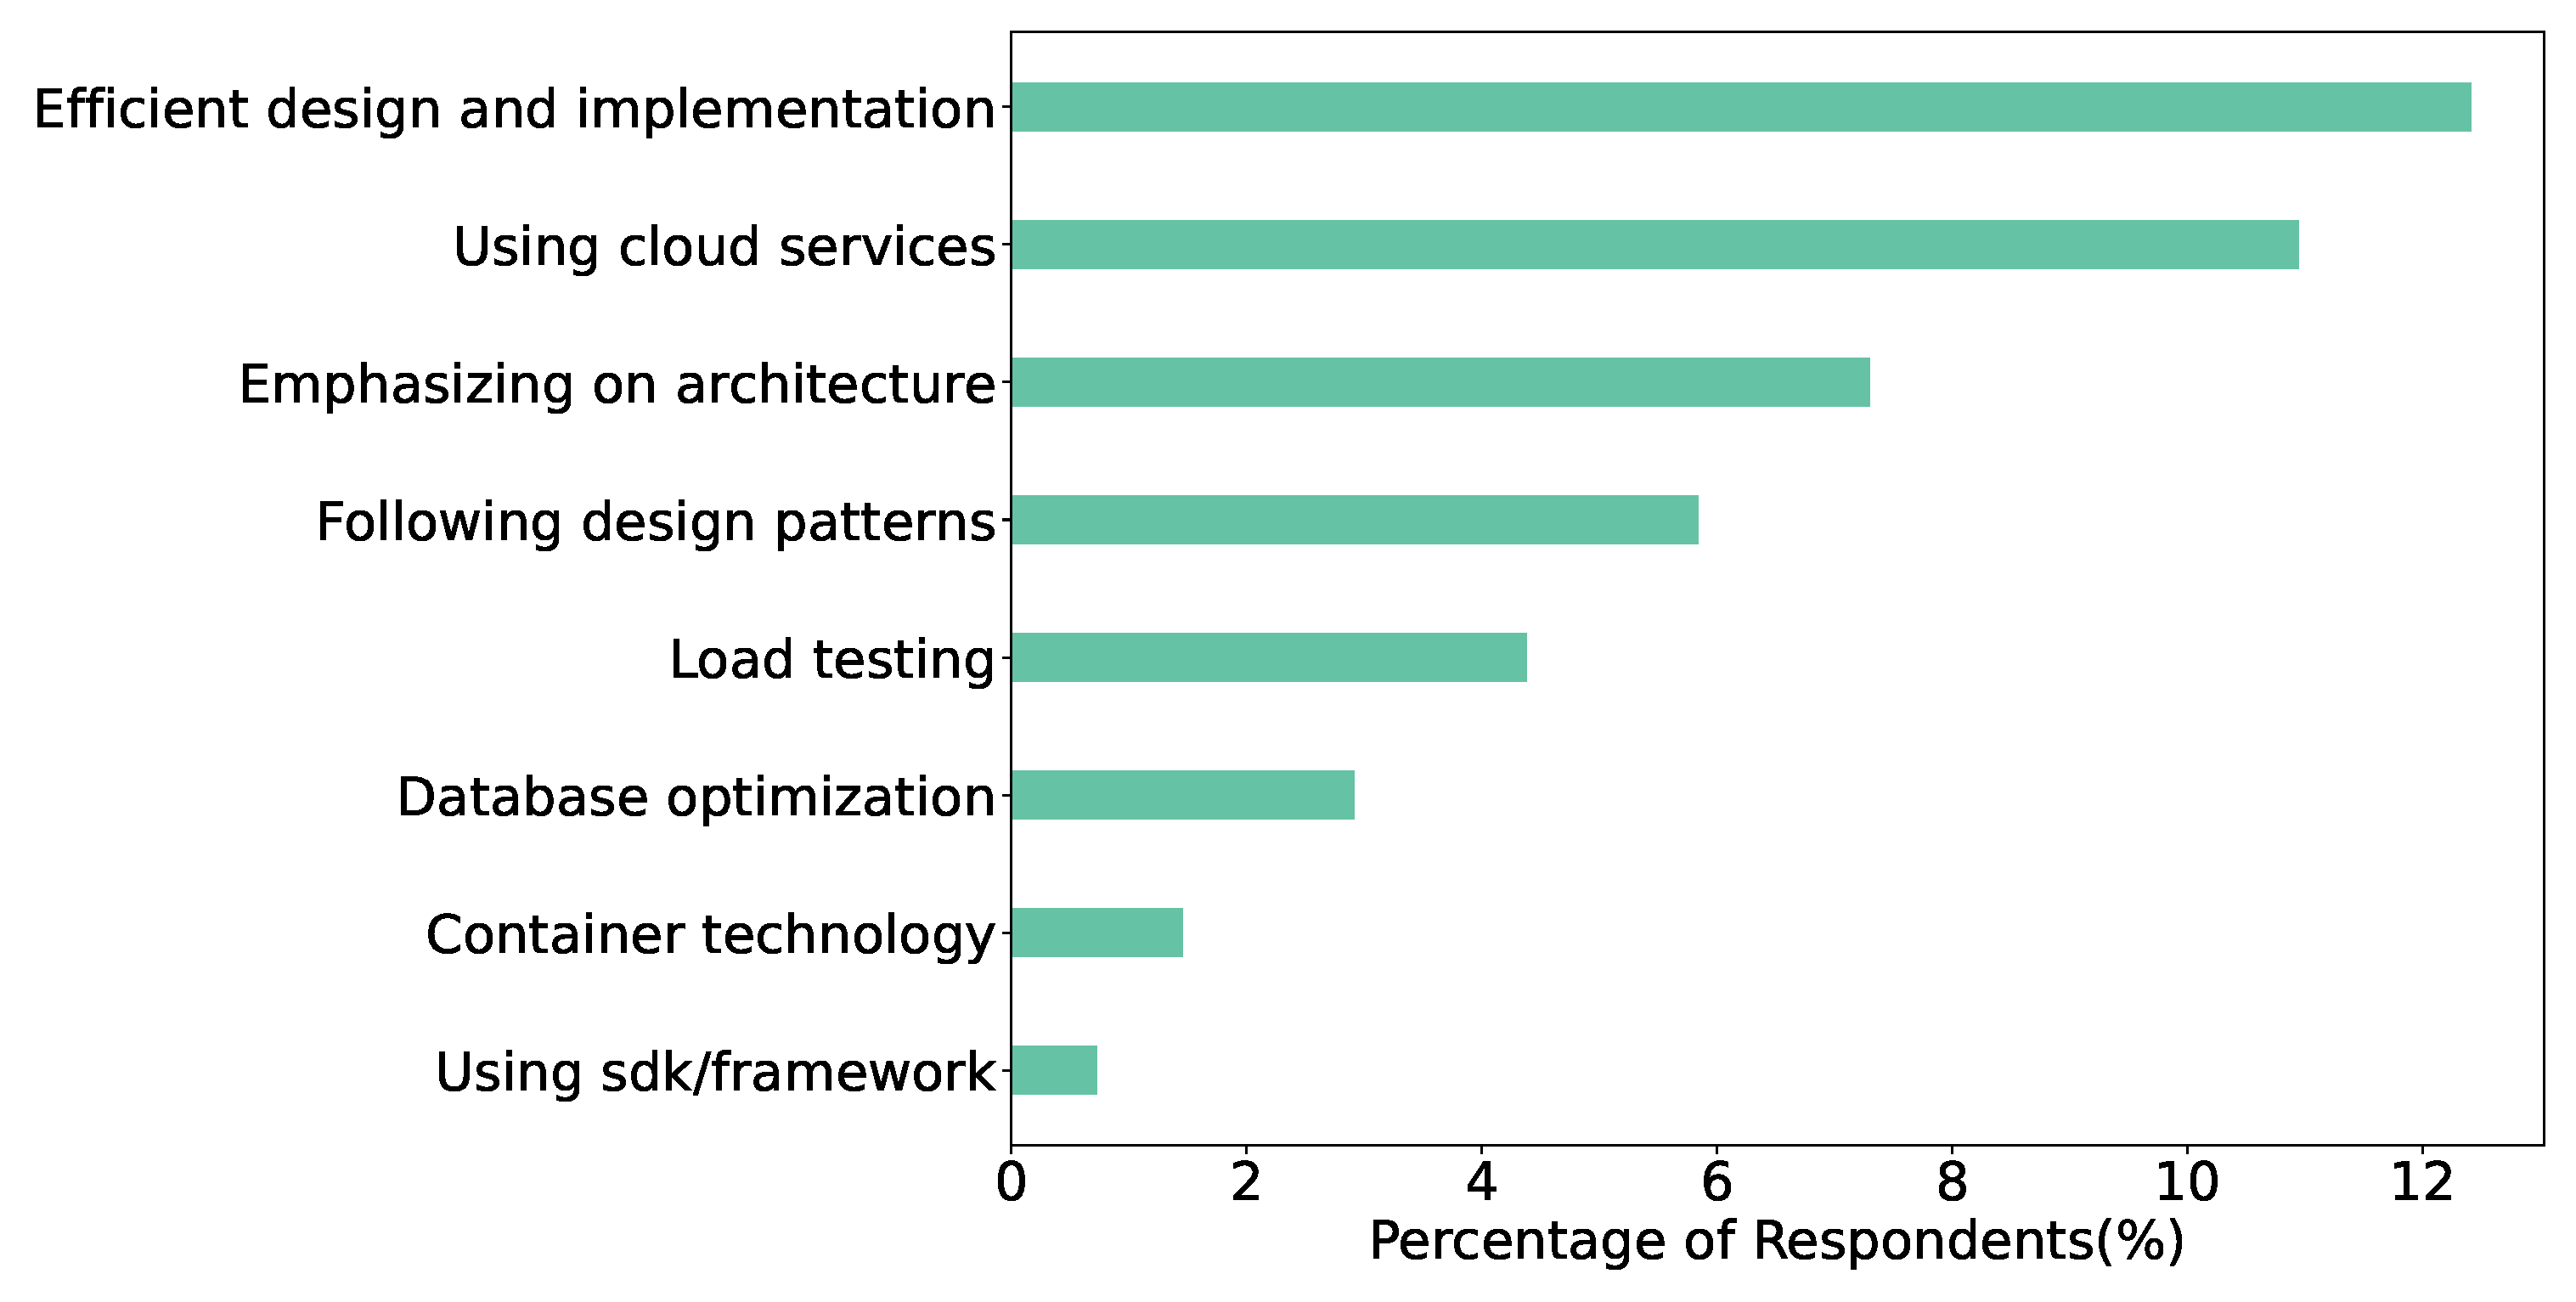
\includegraphics[scale=0.22]{Figures/Scalability.eps} 
% \caption{Measures to ensure scalability of products}
% \label{fig:Measures to ensure scalability}
% \end{figure}
% 
%  Software scalability defines the ability to scale up a solution. Issues with little importance can impede scaling up. Thus proper measures should be taken from the design stage to ensure the scalability of the system. Scalability ensured by efficient software design is the most common strategy in the Bangladesh SE industry. Our open coding of the survey responses reveals four main categories of scalability-related development practices: 
% \begin{inparaenum}
% \item Use of design principles to ensure software scalability (67.3\%).
% \item Exploitation of tools and frameworks to ensure software scalability (34.62\%). 
% \item Use of testing to ensure software scalability(11.54\%), and
% \item Use of database design standards to ensure software scalability (7.69\%).
% \end{inparaenum} 
% The measures practiced in the Bangladesh SE industry are presented in Figure \ref{fig:Measures to ensure scalability}.
% 
% 
%  Scalability ensured by efficient software design is the most common strategy in the Bangladesh SE industry. 67.3\% reported using at least one of the measures in this category. The measures in \emph{efficient software design} category are:
% % Recent days the cloud services offer tools to accomodate custom reactive scaling strategies. Thus, it has become easier to ensure scalability using cloud services \citep{Falatah2014}. Our results  also follows the world trend, usage of cloud services has placed 2\textsuperscript{nd} in terms popularity of scalability measures in SE industry of Bangladesh.
%  \begin{enumerate}[label=(\alph*)]
%  
%      \item \textbf{Efficient Design and Implementation}: 32.69\% of respondents emphasize on the design and implementation of a scalable architecture. 
%     \surveyquote{During implementation we always keep in mind about the scaling factor}{40}
%     
%      \item \textbf{Emphasizing on architecture}: 19.23\% of respondents emphasized on architecture. It is mostly micro-service architecture which they use to ensure scalability.
%     \surveyquote{We follow the micro-service architecture. In a nutshell, we scale up the module vertically which is necessary. We use docker along with Jenkins for automatic deployments and scaling.}{10}
% 
%     
%     \item \textbf{Following Design Patterns}: Some design patterns inherently help in scaling. 15.38\% of respondents think that implementing these design patterns will be of great use for software scalability.
%     \surveyquote{Following certain design patterns}{8}
%  
%  \end{enumerate}
%  
% 34.62\% of respondents of our survey use framework or tool to ensure scalability. The measures in this category are as follows:
% \begin{enumerate}[label=(\alph*)]
% 
%     \item \textbf{Using Cloud Services}: 28.85\% users depend on cloud services such as AWS and Azure for the scalability of the system. Modern features like elastic load balancing and auto-scaling make it easy to ensure scalability.
%     \surveyquote{Using AWS Elastic Load Balancer}{28}
%     
%     \item \textbf{Container Technology}: Container technologies include Docker, Kubernetes, etc. which ensure OS-level virtualization. By standardizing the system, container technologies ease the scaling of infrastructure. 3.85\% of the respondents use these measures to ensure product scalability. Containers enable users to scale their system without any dependency on the underlying OS.
%     \surveyquote{We used Docker technology}{85}
%     
%     \item \textbf{Using SDK/framework}: Modern frameworks ensure scalability by default. 1.92\% of respondents solely depend on the framework for scalability.
%     \surveyquote{following flexible framework which allows better scalability}{14}
%   
% \end{enumerate}
%  
%  
% There is one measure under the software testing category, which is load testing. Load testing can be used to check the scalability of a system. 11.54\% of respondents use load tests to check whether their system is scalable or not.
% \surveyquote{through load testing and load simulation.}{35}
% 
% There is also one measure under the Database Design category, which is database optimization. Database optimization includes sharding, clustering, indexing, and scaling. 7.69\% of respondents optimize the database to scale their system.
% \surveyquote{Besides scaling horizontally, database scaling is performed by partitioning tables, along with multi-threaded implementations}{85}
%\boxtext{Typically software scalability is considered at the design phase in the SE industry of Bangladesh.}
%\boxtext{The use of cloud services is one of the common measures to ensure scalability.}
\begin{tcolorbox}[flushleft upper,boxrule=1pt,arc=0pt,left=0pt,right=0pt,top=0pt,bottom=0pt,colback=white,after=\ignorespacesafterend\par\noindent]
\nd\it{\bf{RQ1-D4. Security and performance measures used.}} Bangladesh software
industry uses various methods to ensure security, but the adoption of tools is not widespread. 
We have noticed that the Bangladesh
software industry mostly uses performance monitoring tools and software testing
to ensure product performance. Software scalability is generally considered at
the design stage (e.g., efficient design) in the Bangladesh SE industry. 
\end{tcolorbox}

\subsection{Comparison of Development Practices Among Countries (RQ2)}
\label{RQ2}
Given Bangladesh is a developing country with a rapidly emerging software development industry, our observations of Bangladesh SE industry can 
offer insights into how such an industry is operating in other similar countries and how such observations 
could differ from countries with matured SE industries. In this section, we offer a comparative assessment of the 
our observations in Bangladesh SE industry against observations reported previously in other countries like 
Canada, Turkey, Netherlands, New Zealand, etc.~\citep{Garousi2013, Garousi2015, Vonken2012, Wang2018}. 
Similar to RQ1, we present the comparisons along four dimensions: \begin{inparaenum}[D1.]
  \item Software development methodologies used (Section \ref{sec:rq2-d1}), 
  \item Software tools and techniques used (Section \ref{sec:rq2-d2}),
\item Software testing and devops practices used (Section \ref{sec:rq2-d3}), and
\item Security and performance measures used (Section \ref{sec:rq2-d4}). 
\end{inparaenum}
The summary of the comparison is presented in Table~\ref{table:comparison_summary}.
%   
% This section presents a comparative discussion on different dimensions of software development practices and processes among different regions of the world along with Bangladesh. We make the comparison along the following dimensions:
% 
% \begin{itemize}
% \item Development methods and practices
% \item Implementation technologies
% \item Quality assurance
% \item Release and iterations
% \end{itemize}
% 
% The following subsections describe these dimensions.

\subsubsection{Development methods and practices}
\label{dev_methods}

To find out the overall comparison of this section, we report the following sub-sections:

\begin{itemize}
\item Software development methodologies (Q 6).
\item Requirements gathering (Q 7).
\item Most time consuming software development activities (Q 8).
\end{itemize}

\paragraph{Software development methodologies}
From the study we see that the most acceptable model that was regularly and always used is the agile model (64\%) in Bangladesh but the usage of the scrum (44\%) in New Zealand has greater usage followed by agile (30\%) \cite{Wang2018} and in Turkey, waterfall is mostly used based on the earlier 2015 survey \cite{Garousi2015}. Again, in both Bangladesh and New Zealand, extreme programming (XP) has a lower percentage of usage.

\paragraph{Requirements Gathering}
According to \ref{fig:requirements}, using plain text (44\%) and story board (41\%) are the most widely used requirements gathering. This result is similar with the survey of Vonken et al. \cite{Vonken2012}. From their study we can find that the textual description of specifying requirements is a firm favourite in Netherlands.

\paragraph{Development activities timeline}
According to study \cite{Wang2018}, most time was spent on implementation and coding and also relatively less time was spent on maintenance in both Bangladesh and New Zealand. But requirement analysis, the activity, requires the second most time to spend in Bangladesh according to 45\% respondents where in New Zealand, it is testing (36\%) practices.

\subsubsection{Software development tools and techniques used (D2)} \label{sec:rq2-d2}
% \begin{table}[!ht]
\caption{Comparison of tech platforms, OS and programming languages between our findings and prior findings}
\begin{tabular}{llll}

\hline
\multicolumn{1}{c}{\textbf{Practices}} & \multicolumn{1}{c}{\textbf{Our Study}} & \multicolumn{1}{c}{\textbf{Prior Study}} & \multicolumn{1}{c}{\textbf{Comparison}}\\ 
\hline 


\multicolumn{1}{l|}{\multirow{3}{*}{\parbox{0.14\textwidth}{Which implementation technologies and tools are adopted by software development professionals?}}
} 

&

\multicolumn{1}{l|}{\multirow{3}{*}{\parbox{0.26\textwidth}{
\vspace{-45pt} (1) Majority of our participants were related to the various types of web-based applications that convey the market demand for web-based apps in Bangladesh. (2) Linux is mainly used for development purposes while macOS is highly preferred by managers. (3) Javascript and Java are two mostly used programming languages in the Bangladesh SE industry since the demand for web-based services as well as mobile apps.
}}} 
& 
\multicolumn{1}{l|}{\comparisoncell{0.25}{{\vspace{40pt} There exists a high level focus on web-based platforms in the software industry of New Zealand \citep{Wang2018}.
}}}
& 
\multirow{3}{*}{\parbox{0.21\textwidth}{
We have observed that web-based platforms have widespread demand among different countries along with Bangladesh. Besides, in using programming languages like Java and python, Bangladesh has similarities with Turkey but is different from New Zealand.
}} \\ \cline{3-3}

\multicolumn{1}{l|}{}                                       
& 
\multicolumn{1}{l|}{}                                       
& 

\multicolumn{1}{l|}{\comparisoncell{0.25}{{
\vspace{40pt} Windows is highly preferable among developers of New Zealand \citep{Wang2018}.
}}}                                                         
&                                                       
\\ \cline{3-3}

\multicolumn{1}{l|}{}               
& 
\multicolumn{1}{l|}{}                                        
& 

\multicolumn{1}{l|}{\comparisoncell{0.25}{
\vspace{40pt} The use of Java as a programming language is spacious in Turkey \citep{Garousi2015}. However, in New Zealand, the usage rate of Java, as well as python ranks somewhat low \citep{Wang2018}.
}} 
&                                                           
\\ \hline

\end{tabular}
\label{table:tech_comparison}
\end{table}

We compare our observations from three questions: \begin{inparaenum}
\item Technology Platform (Q9).
\item Operating System (Q10).
\item Programming Language (Q11).
%\item Framework (Q12).
%\item IDE (Q13).
\end{inparaenum} The observations from two questions (Programming language Q11 and IDE used Q12) could not be compared, because 
those were not previously asked in the context of other countries. The comparisons are discussed below.

% To find out the overall comparison of this section, we report the following sub-sections:
% \begin{itemize}
% \item Technology Platform (Q9).
% \item Operating System (Q10).
% \item Programming Language (Q11).
% \end{itemize}
% 
% We have compared our study findings on these sub-topics to get similarities and dissimilarities with the countries like Turkey, New Zealand, etc., on which a couple of relevant studies have been conducted. We compare the major findings of our study with the similar findings of previous studies in Table \ref{table:tech_comparison}.
%\paragraph{Technology Platforms}

\nd\bf{$\bullet$ Technology platforms (Q9).} As shown in
Figure~\ref{fig:platforms}, most of our survey respondents (80\%) work in web
platforms. This outcome is similar to the result of the survey of Wang et al.
\citep{Wang2018} in which the authors found that most of their respondents also
develop in web platforms in New Zealand.


%\paragraph{Operating Systems}
\nd\bf{$\bullet$ Operating Systems (Q10).} We have found an interesting point
that Windows is mostly used among developers of New Zealand based on the study
\citep{Wang2018} nevertheless, Linux is mostly used in the case for Bangladeshi
developers corresponding to our survey presented in Figure~\ref{fig:os}.

%\paragraph{Programming Languages}
\nd\bf{$\bullet$ Programming Languages (Q11).} According to the study of Wang et
al.\citep{Wang2018}, Java ranks quite low in New Zealand; nevertheless, it is
the second most used programming language in Bangladesh as per our study
reported in Figure~\ref{fig:languages} as well as the most used language in
Turkey \citep{Garousi2015}. Again, Python did not have a good standing in the
ranking of languages used in New Zealand; nevertheless, it is used significantly
in Bangladesh.

\begin{tcolorbox}[flushleft upper,boxrule=1pt,arc=0pt,left=0pt,right=0pt,top=0pt,bottom=0pt,colback=white,after=\ignorespacesafterend\par\noindent]
\nd\it{\bf{RQ2-D2. Software development tools and techniques used.}}
Like other SE industries, the web is the main technology platform in Bangladesh.
Linux is the preferred OS in Bangladesh's SE industry, while it is  Windows in 
New Zealand SE industry. Although Java and Python are popular languages in the
SE industry in Bangladesh, we have noticed that they are not very popular in the
New Zealand SE industry.
\end{tcolorbox}
\subsubsection{What type of testing and deployment practices are used?}

To get the picture of quality assurance (QA) in countries such as Malaysia, Turkey, France, etc., different studies have been carried out. In Table \ref{table:testing_comparison}, we compare the major outcomes of testing and deployment related responses from our study with the similar results of the previous studies. The comparative picture is discussed below.

\begin{itemize}
    % \item Requirements Clarity
    \item Software Testing Practices (Q14)
    \item Level of Automated Testing (Q15)
\end{itemize}

\begin{table}[]
\caption{Comparison of testing practices and test automation between our findings and prior findings}

\begin{tabular}{llll}

\hline
\multicolumn{1}{c}{\textbf{Practices}} & \multicolumn{1}{c}{\textbf{Our Study}} & \multicolumn{1}{c}{\textbf{Prior Study}} & \multicolumn{1}{c}{\textbf{Comparison}} \\ 
\hline 


\multicolumn{1}{l|}{\multirow{2}{*}{\parbox{0.1\textwidth}{What type of testing and deployment practices are used?}}
} 
& 
\multicolumn{1}{l|}{\multirow{2}{*}{\parbox{0.25\textwidth}{
\vspace{-50pt} (1) Around half of our respondents responded about carrying out unit testing and functional testing. Also, the utilization rate of acceptance and UI testing has an appreciable percentage in Bangladesh. (2) Automated testing exercise is not usual in Bangladesh as per the majority of our respondents.
}}
} 
& 
\multicolumn{1}{l|}{\comparisoncell{0.25}{\vspace{50pt}Unit testing is observed to be the most exercised in Malaysia (68.29\%) \citep{Baharom2006}, Canada (79.27\%) \citep{Garousi2013}, New Zealand (73\%) \citep{Wang2018} in a great percentage.
}}                                  

&

\multirow{2}{*}{\parbox{0.23\textwidth}{
\vspace{-70pt} We have perceived that unit testing is moderately practiced in Bangladesh, though its usage is comparatively spacious in other countries. In the adoption of test automation, the software industry of Bangladesh is way behind France though the usage rate might have similar to other European countries.
}} \\ \cline{3-3}

\multicolumn{1}{l|}{}                                       
& 
\multicolumn{1}{l|}{}                                       
& 

\multicolumn{1}{l|}{\comparisoncell{0.25}{
\vspace{50pt} Test automation is highly embraced by France software industry and comparatively less adopted in overall Europe~\citep{dutta1999}.
}} 
&                                         
\\ \hline

\end{tabular}
\label{table:testing_comparison}
\end{table}



\paragraph{Software Testing Practices}
From our study, as per \ref{fig:testing}, we see an interesting point that unit testing (53\%) and functional testing (49\%) are moderately used in Bangladesh, whereas from \citep{Garousi2013} and \citep{Wang2018} we can see that relatively a high percentage of their survey respondents in both Canada New Zealand rely on unit testing with 79.27\% and 73\% respectively. On the other hand, the adoption of acceptance testing and UI testing is quite similar to these countries. In Malaysia, based on \citep{Baharom2006}, Baharom et al. reported that, according to their survey, unit testing (68.29\%), integration testing (78.05\%), system testing (85.37\%), and acceptance testing (78.05\%) are used by most organizations in a high percentage, and about half of the organizations are carrying out alpha and beta testing.

\boxtext{Software developers around the world usually give unit testing the top priority, but the developers in Bangladesh have comparatively less participation.}
\rifat{Is the above observation correct? 53\% usage of unit testing reported.}\khalid{added percentages. The response rate of unit testing in our survey lags compares to others. Is it okay now?}

\paragraph{Level of Automated Testing}
We have found that as per \ref{fig:autoTest}, around 25\% of our respondents are highly concerned that they have to use automated testing for their projects, while around 35\% of our respondents have expressed medium level concern and the remaining are hardly concerned about using automated testing. From the study of Dutta et al. \citep{dutta1999}, we have found that in automated testing practices, Bangladesh is quite similar to all of Europe but lags behind France. According to their study, the usage rate of automation testing tools in overall Europe is 26\%, where in France, it is as high as 61\%. But in Israel, this rate is the only 9\%.

\begin{tcolorbox}[flushleft upper,boxrule=1pt,arc=0pt,left=0pt,right=0pt,top=0pt,bottom=0pt,colback=white,after=\ignorespacesafterend\par\noindent]
\nd\it{\bf{RQ2-D3. Software testing and devops practices used.}} 
\gias{summarize}
\end{tcolorbox}

% \subsubsection{Release and Iterations}
\label{vcs_comparison}

\subsubsection{How are the security and performance ensured in the products of a company?}

Several studies have been performed to identify security and performance practices in countries like Canada, New Zealand, and Turkey. We have found some differences as well as similarities in the practices of those countries with others. In Table \ref{table:open_ended_comparison}, we compare the major findings of our study against the findings of previous studies.

% Please add the following required packages to your document preamble:
% \usepackage{multirow}
\begin{table}[!ht]
\caption{Comparison of security, performance, scalability between our findings and prior findings}
\begin{tabular}{llll}

\hline
\multicolumn{1}{c}{\textbf{Practices}} & \multicolumn{1}{c}{\textbf{Our Study}} & \multicolumn{1}{c}{\textbf{Prior Study}} & \multicolumn{1}{c}{\textbf{Comparison}} \\ 
\hline

\multicolumn{1}{l|}{\multirow{3}{*}{\parbox{0.1\textwidth}{
How are the security and performance is ensured in a product of a company?
}}}

&

\multicolumn{1}{l|}{\multirow{3}{*}{\parbox{0.22\textwidth}{
(1) The practice of security architecture and security testing as a security measure are not prevalent in the Bangladesh SE industry. (2) Performance testing and peer review are the two least practiced performance measure in the Bangladesh SE industry. (3) Cloud service and architecture are two of the top three scalability measures.
}}} 

&

\multicolumn{1}{l|}{\comparisoncell{0.30}{
\vspace{13pt} Security testing is found to be the least practiced in the software industry in Turkey\citep{Garousi2015}, Malaysia\citep{Farvin2016}, India\citep{Bahl2011}, and New Zealand\citep{Sung2006}
}}                                                          

& 

\multirow{3}{*}{\parbox{0.22\textwidth}{
We found that the practice of `no security' measures is less in Bangladesh compared to other countries. Though the practice of security testing Bangladesh has similarities with other countries, it lags behind the practices of matured industries. However, like the matured and grown software industries, cloud service is a popular measure in Bangladesh.
}} 
\\ \cline{3-3}

\multicolumn{1}{l|}{}                                       
& 
\multicolumn{1}{l|}{}                                       
&

\multicolumn{1}{l|}{\comparisoncell{0.30}{
\vspace{13pt} Performance testing is a common practice in some \citep{Garousi2013,Garousi2015,Phillips2003} SE industry. However, it is hardly practiced in the Pakistan\citep{Jahan2019} SE industry. Also, peer review is a common practice among Turkish\citep{Garousi2015} developers.
}}                                                          

& 
\\ \cline{3-3}
\multicolumn{1}{l|}{}                                       
& 
\multicolumn{1}{l|}{}  
& 

\multicolumn{1}{l|}{\comparisoncell{0.30}{
\vspace{13pt} To ensure scalability, there are many practices prevalent in other countries' SE industry, such as micro-service architecture\citep{Laihonen2018} and containerization technologies\citep{Hussain2017}.
}} 
& 
\\ \hline


\end{tabular}
\label{table:open_ended_comparison}
\end{table}

\label{security_comparison}
A very few percentages (3.64\%) of our survey respondents reported not to use any security measures in their product. This practice is also prevalent in the Indian and Malaysian software industries. Bahl et al.\citep{Bahl2011} reported that due to misalignment with organization design, goal, and strategy in some Indian software firms, security measures are not practiced. In a study with Malaysian developers, Farvin et al.\citep{Farvin2016} found that 31\% of respondents think it is not required to add security in the requirement analysis of a product. Basharat et al.\citep{Basharat2013} reported a sense of false security in the small software industry and standard security practices are hardly followed. It is likely to be applicable to the industry in Bangladesh as well. From the response of a survey on the Turkish software industry, Garousi et al.\citep{Garousi2015} ranked different design activities in terms of frequency. Security architecture was ranked second out of five (five is for always used activities and one is for never used activities). The ranking represents that security architecture is not a frequent activity in the Turkish software industry. However, in our survey, we see very few respondents reported to practice security design principles while designing system architecture. Our survey found that 2.19\% of respondents rely on security architecture/security design principles to ensure security in their product. The software industries of Bangladesh, Turkey, and New Zealand have a resemblance in the practice of security testing. Garousi et al.\citep{Garousi2015} reported that security testing is least widely used among all kinds of testing (e.g., unit testing, integration testing). Sung et al.\citep{Sung2006} found that in the New Zealand software industry, security testing and recovery testing practices are negligible compared to functional testing. The scenario is the same for Bangladesh; we found that 6.57\% of respondents reported security testing to ensure security.


% \subsubsection{Performance measures}
% \label{performance_comparison}
8.76\% respondents of our survey use performance testing to ensure the performance of their product. \anindya{Should we say respondents or the companies they work? Think about it as we mention this at different places.}\partha{The survey question was `How do you ensure security of your products?' participants may answer this question from both personal and company perspective. It seems to me that the goal was to find out the participants' security practices. What do you suggest?} However, it is the second least practiced measure among all the measures. Garousi et al.\citep{Garousi2015} found that developers mark the lack of performance testing as the main challenge in software maintenance in the Turkish software industry. However, the scenario is different for the Canadian software industry. Participants of the survey of Garousi et al.\citep{Garousi2013} reported that 40\% of them conduct performance testing, and 30\% of their total testing effort is spent on performance testing. The New Zealand software industry follows the practice similar to Canada as reported by Phillips et al.\citep{Phillips2003}. %reported that performance testing is a common testing practice in New Zealand.
The practice in Bangladesh matches that of Pakistan. 
%In Pakistan software industry, performance testing is hardly practiced.
In the survey of Shah Jahan et al.\citep{Jahan2019}, only 5\% of participants reported conducting performance testing. It seems that performance testing is less popular in growing software industries such as Bangladesh and Pakistan.

Peer review is the least practiced measure in the Bangladesh software industry. However, in the Turkish software industry, peer review is ranked as the most frequent activity\citep{Garousi2015} (ranked five on a five-point Likert scale), though the practice is only limited to code review. Architecture/design review is hardly practiced in turkey (ranked one on a five-point Likert scale). We found that peer review is limited to only code review in the Bangladeshi software industry, and the only 2.92\% of our participants reported practicing peer review.

% \subsubsection{Scalability measures}
% \label{scalability_comparison}
There is no study focusing on scalability practices in specific software industries, so it isn't easy to compare scalability practices. However, in a study on Finnish DevOps, Laihonen\citep{Laihonen2018} found that the Finnish software industry prefers cloud services as it helps them automate quality assurance. He also reported that DevOps is inclined towards micro-service architecture when selecting a product rather than monolithic architecture. Hussain et al.\citep{Hussain2017} conducted a study to identify trends in the DevOps practices in New Zealand. For this study, besides interviewing the DevOps, they examined the job advertisements for a DevOps role. They found that containerization technologies (e,g., Docker, Kubernetes) have a high demand in the New Zealand software industry. 94\% of job advertisement requires expertise in one or multiple containerization technologies. This indicates the popularity of docker technology in the New Zealand software industry. However, in the Bangladeshi software industry, the scenario is different. Cloud services are the second most popular (10.95\%) measure to ensure scalability where the use of containerization technologies are not that much popular (1.46\%)

\begin{tcolorbox}[flushleft upper,boxrule=1pt,arc=0pt,left=0pt,right=0pt,top=0pt,bottom=0pt,colback=white,after=\ignorespacesafterend\par\noindent]
\nd\it{\bf{RQ2-D4. Security and performance measures used.}} \gias{summarize RQ2-D4 here}
\end{tcolorbox}




% \subsection{Development Practices and Processes in Bangladesh (RQ1)}
\label{RQ1}

We divide this into following four sub-questions which examine software development practices and processes in Bangladesh in more detail.

\subsubsection{What software methodology are used in your project?}
\label{methodology}
Software development methodology in software engineering is a framework that is used to pursue the development of information systems in a very deliberate, structured and methodical way. To find out the overall answer of this question, we report the following results:
\begin{itemize}
\item Software development methodologies (Q 6).
\item Requirements gathering (Q 7).
\item Most time consuming software development activities (Q 8).
\end{itemize}

\paragraph{Software development methodologies}
The most-widely used model is Agile with usage rate of 64\%. The next widely-used model is scrum with usage rates of 46\%. The other methodologies has lower usage rates, namely: pair programming (20\%), Waterfall (12\%) etc.

% \begin{figure}[htbp]
% \centering
%   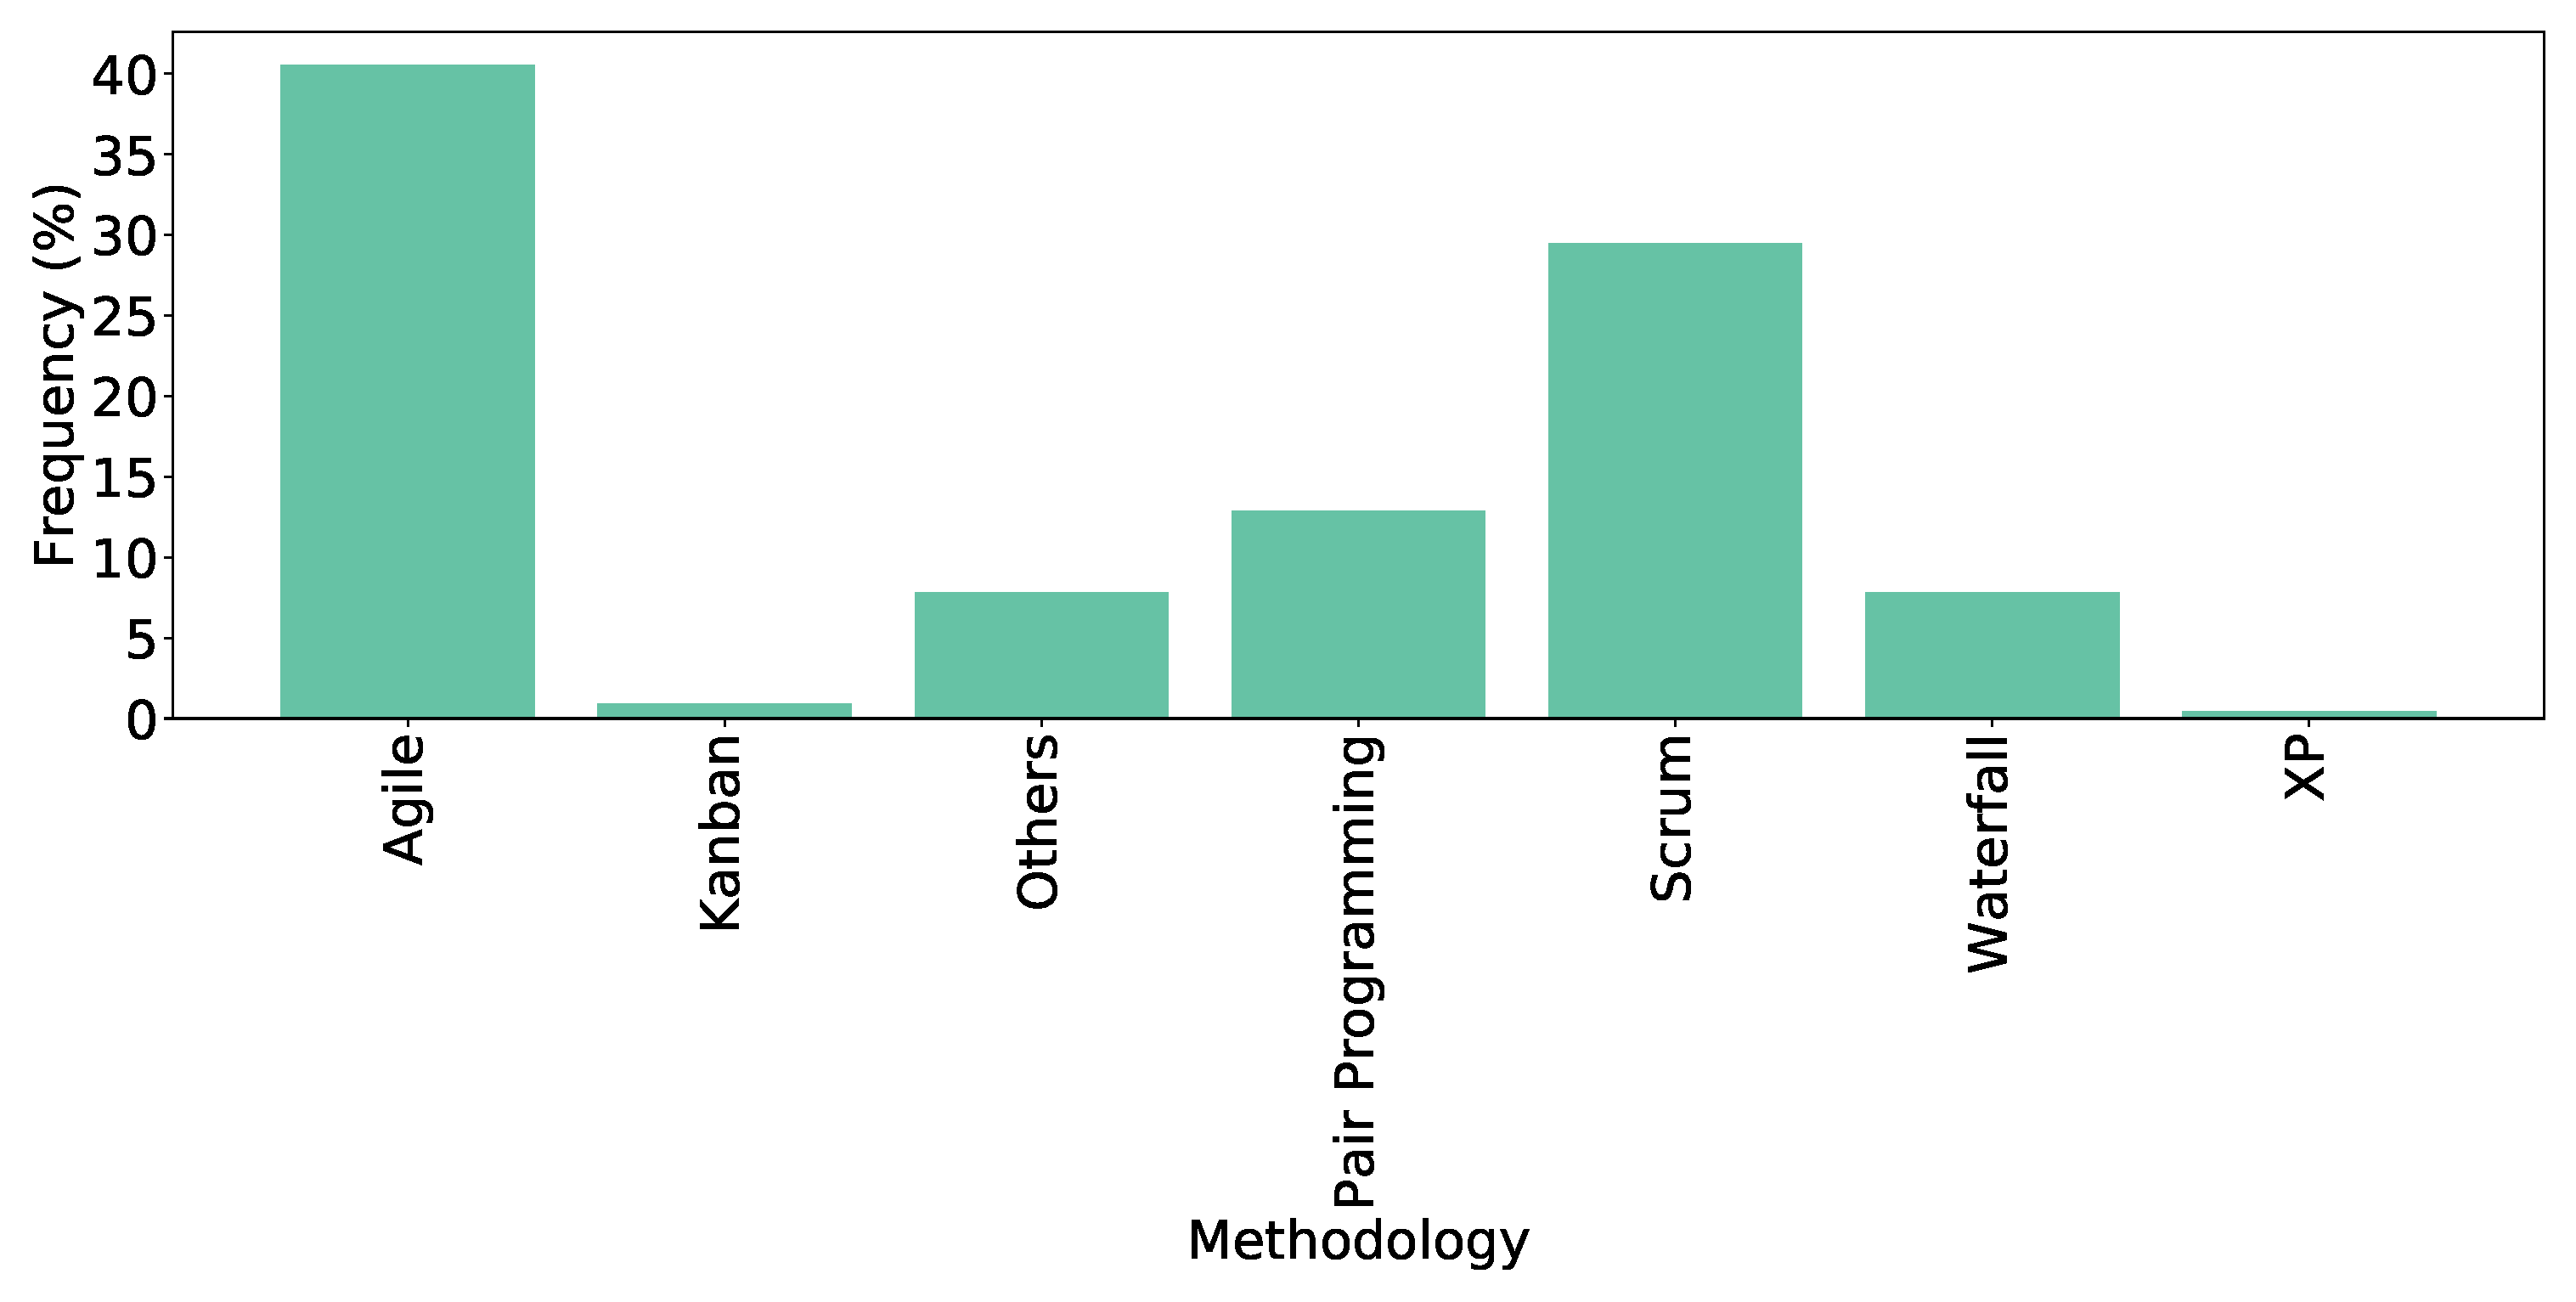
\includegraphics[width=0.8\textwidth]{Figures/Respondents_Methodology}
%   \caption{Software development methodologies}
%   \label{fig:methodologies}
% \end{figure}

\paragraph{Requirements Gathering}
The most critical activity that always arises during software development is the collecting requirement of the proposed system. According to \ref{fig:requirements}, using plain text (44\%) and story board (41\%) are the most widely used requirements gathering. The other requirements gathering usage rates are: Use case (36\%), GUI prototype (35\%), grooming session (30\%) etc. This is an important finding that requires further analysis for causes and to analyze the potential effects of not documenting requirements.

% \begin{figure}[htbp]
% \centering
%   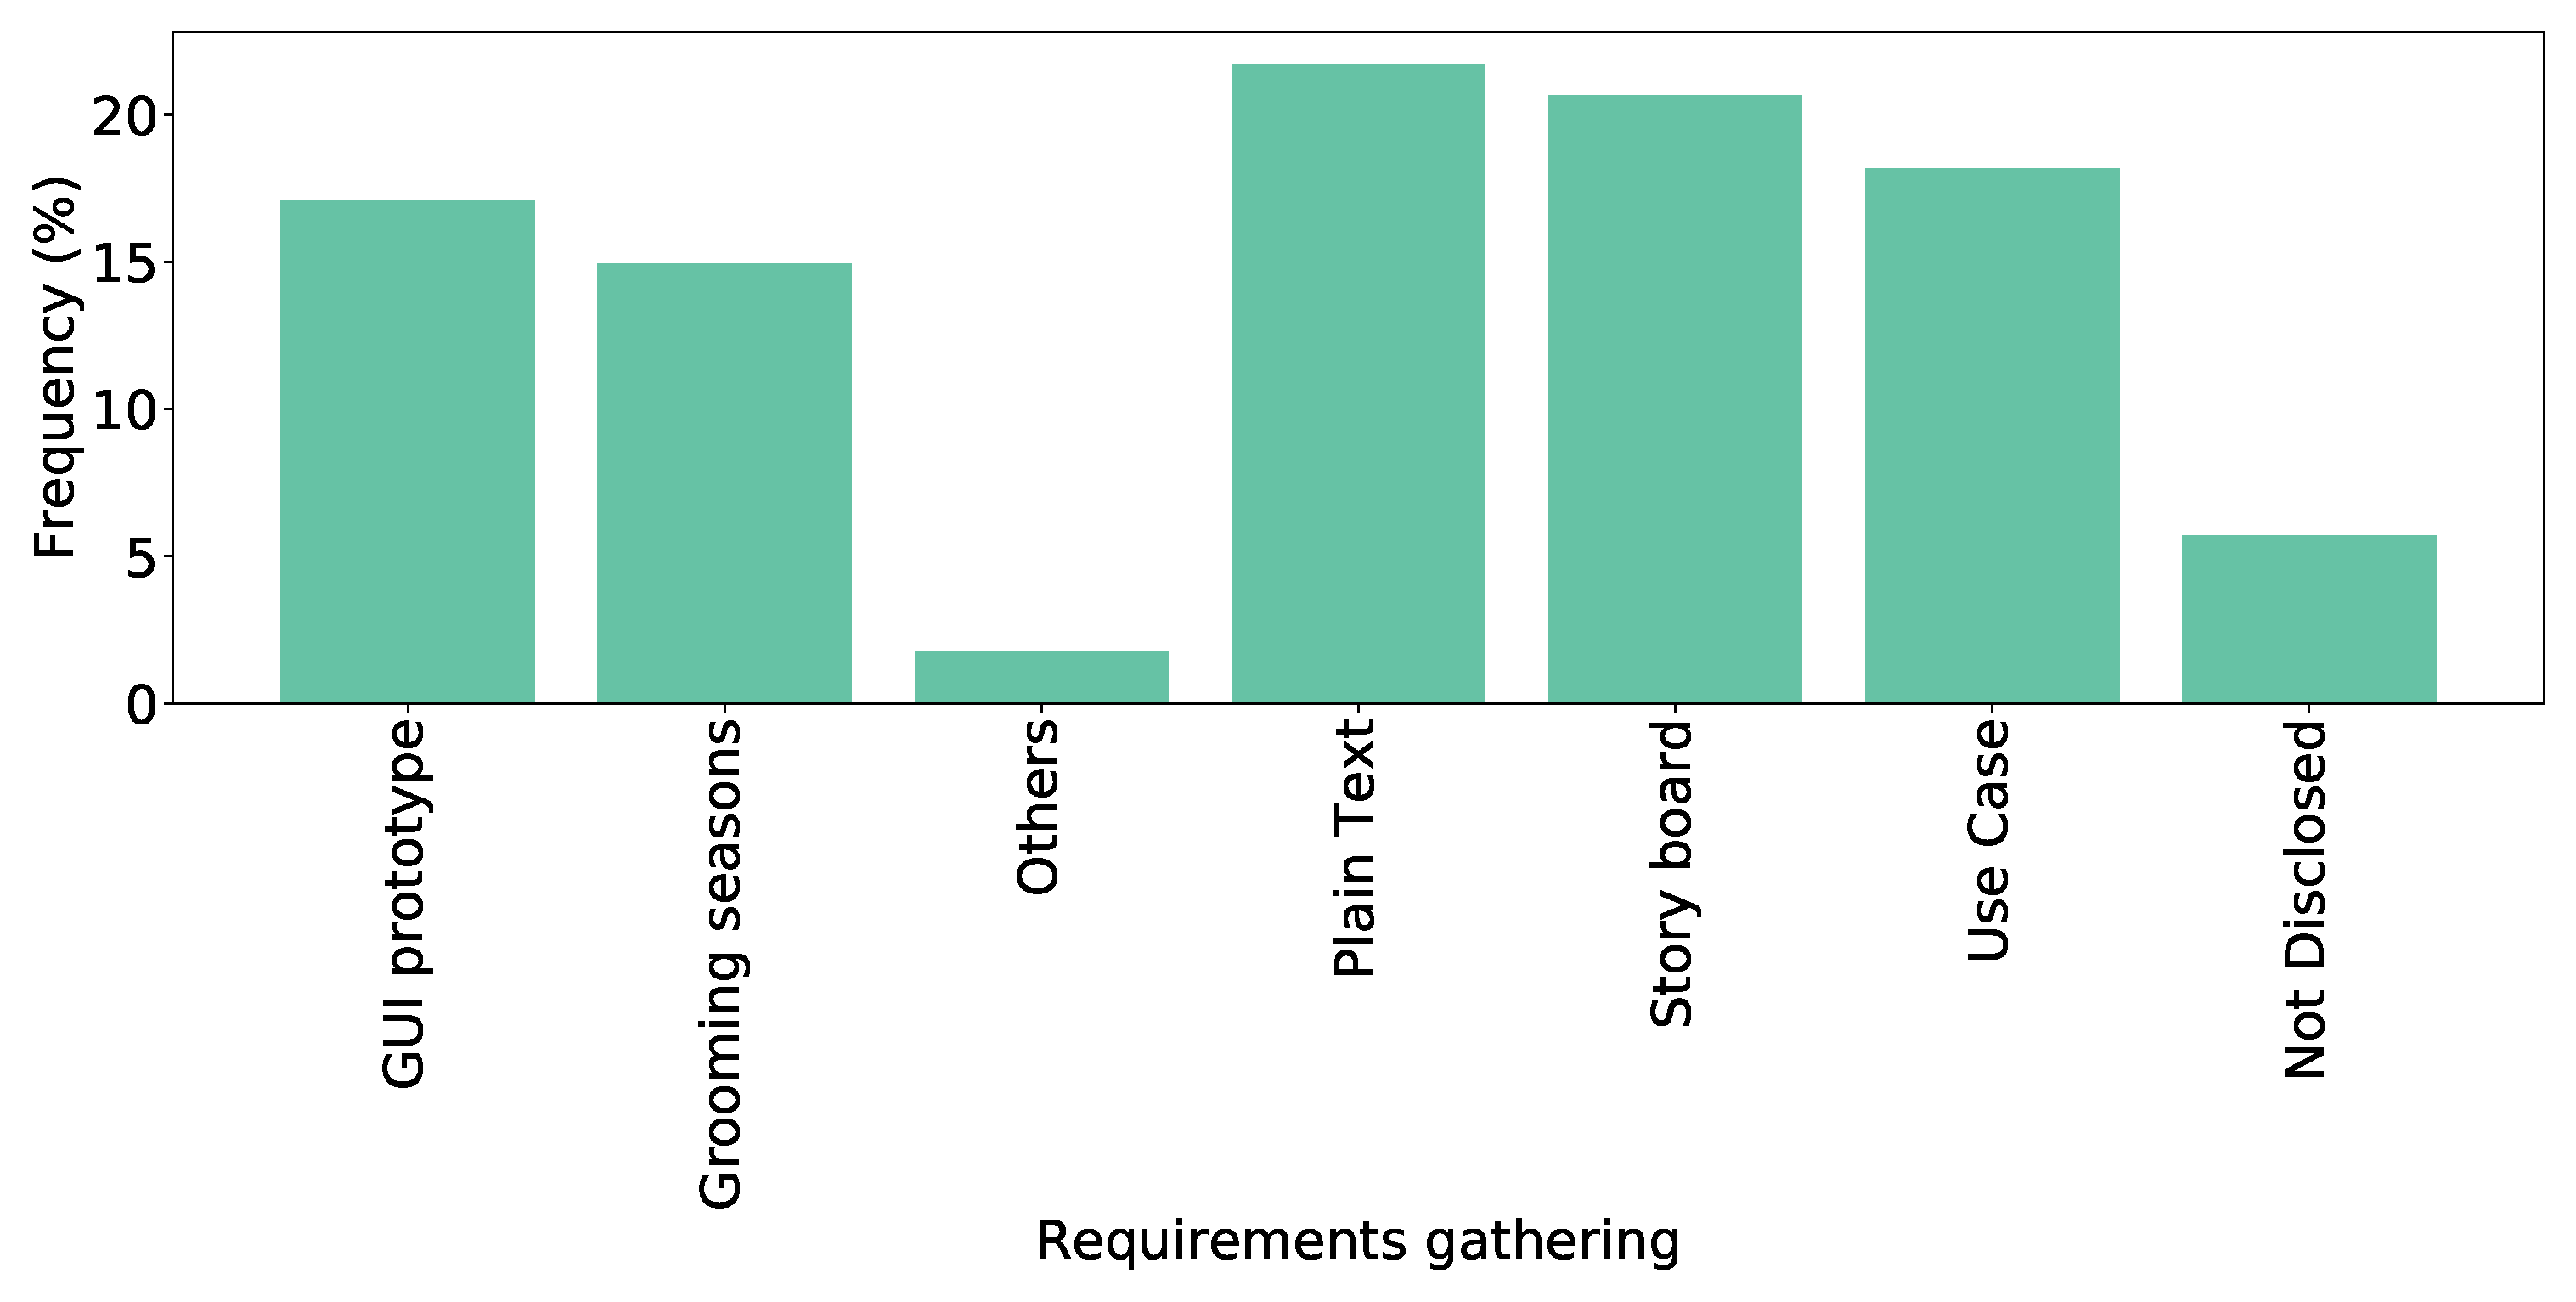
\includegraphics[width=0.8\textwidth]{Figures/Requirements_Gathering}
%   \caption{Requirements gathering}
%   \label{fig:requirements}
% \end{figure}

\paragraph{Development activities timeline}
In this section participants were asked about the most time consuming software developing activities they had spend. As we see in \ref{fig:activities}, most of the time spent in implementation stage according to 65\% our respondents and requirement analysis stage requires second most according to 45\% response. The other usages are: Program design (37\%), project planning (30\%), testing (19\%), maintenance (17\%) etc.

% \begin{figure}[htbp]
% \centering
%   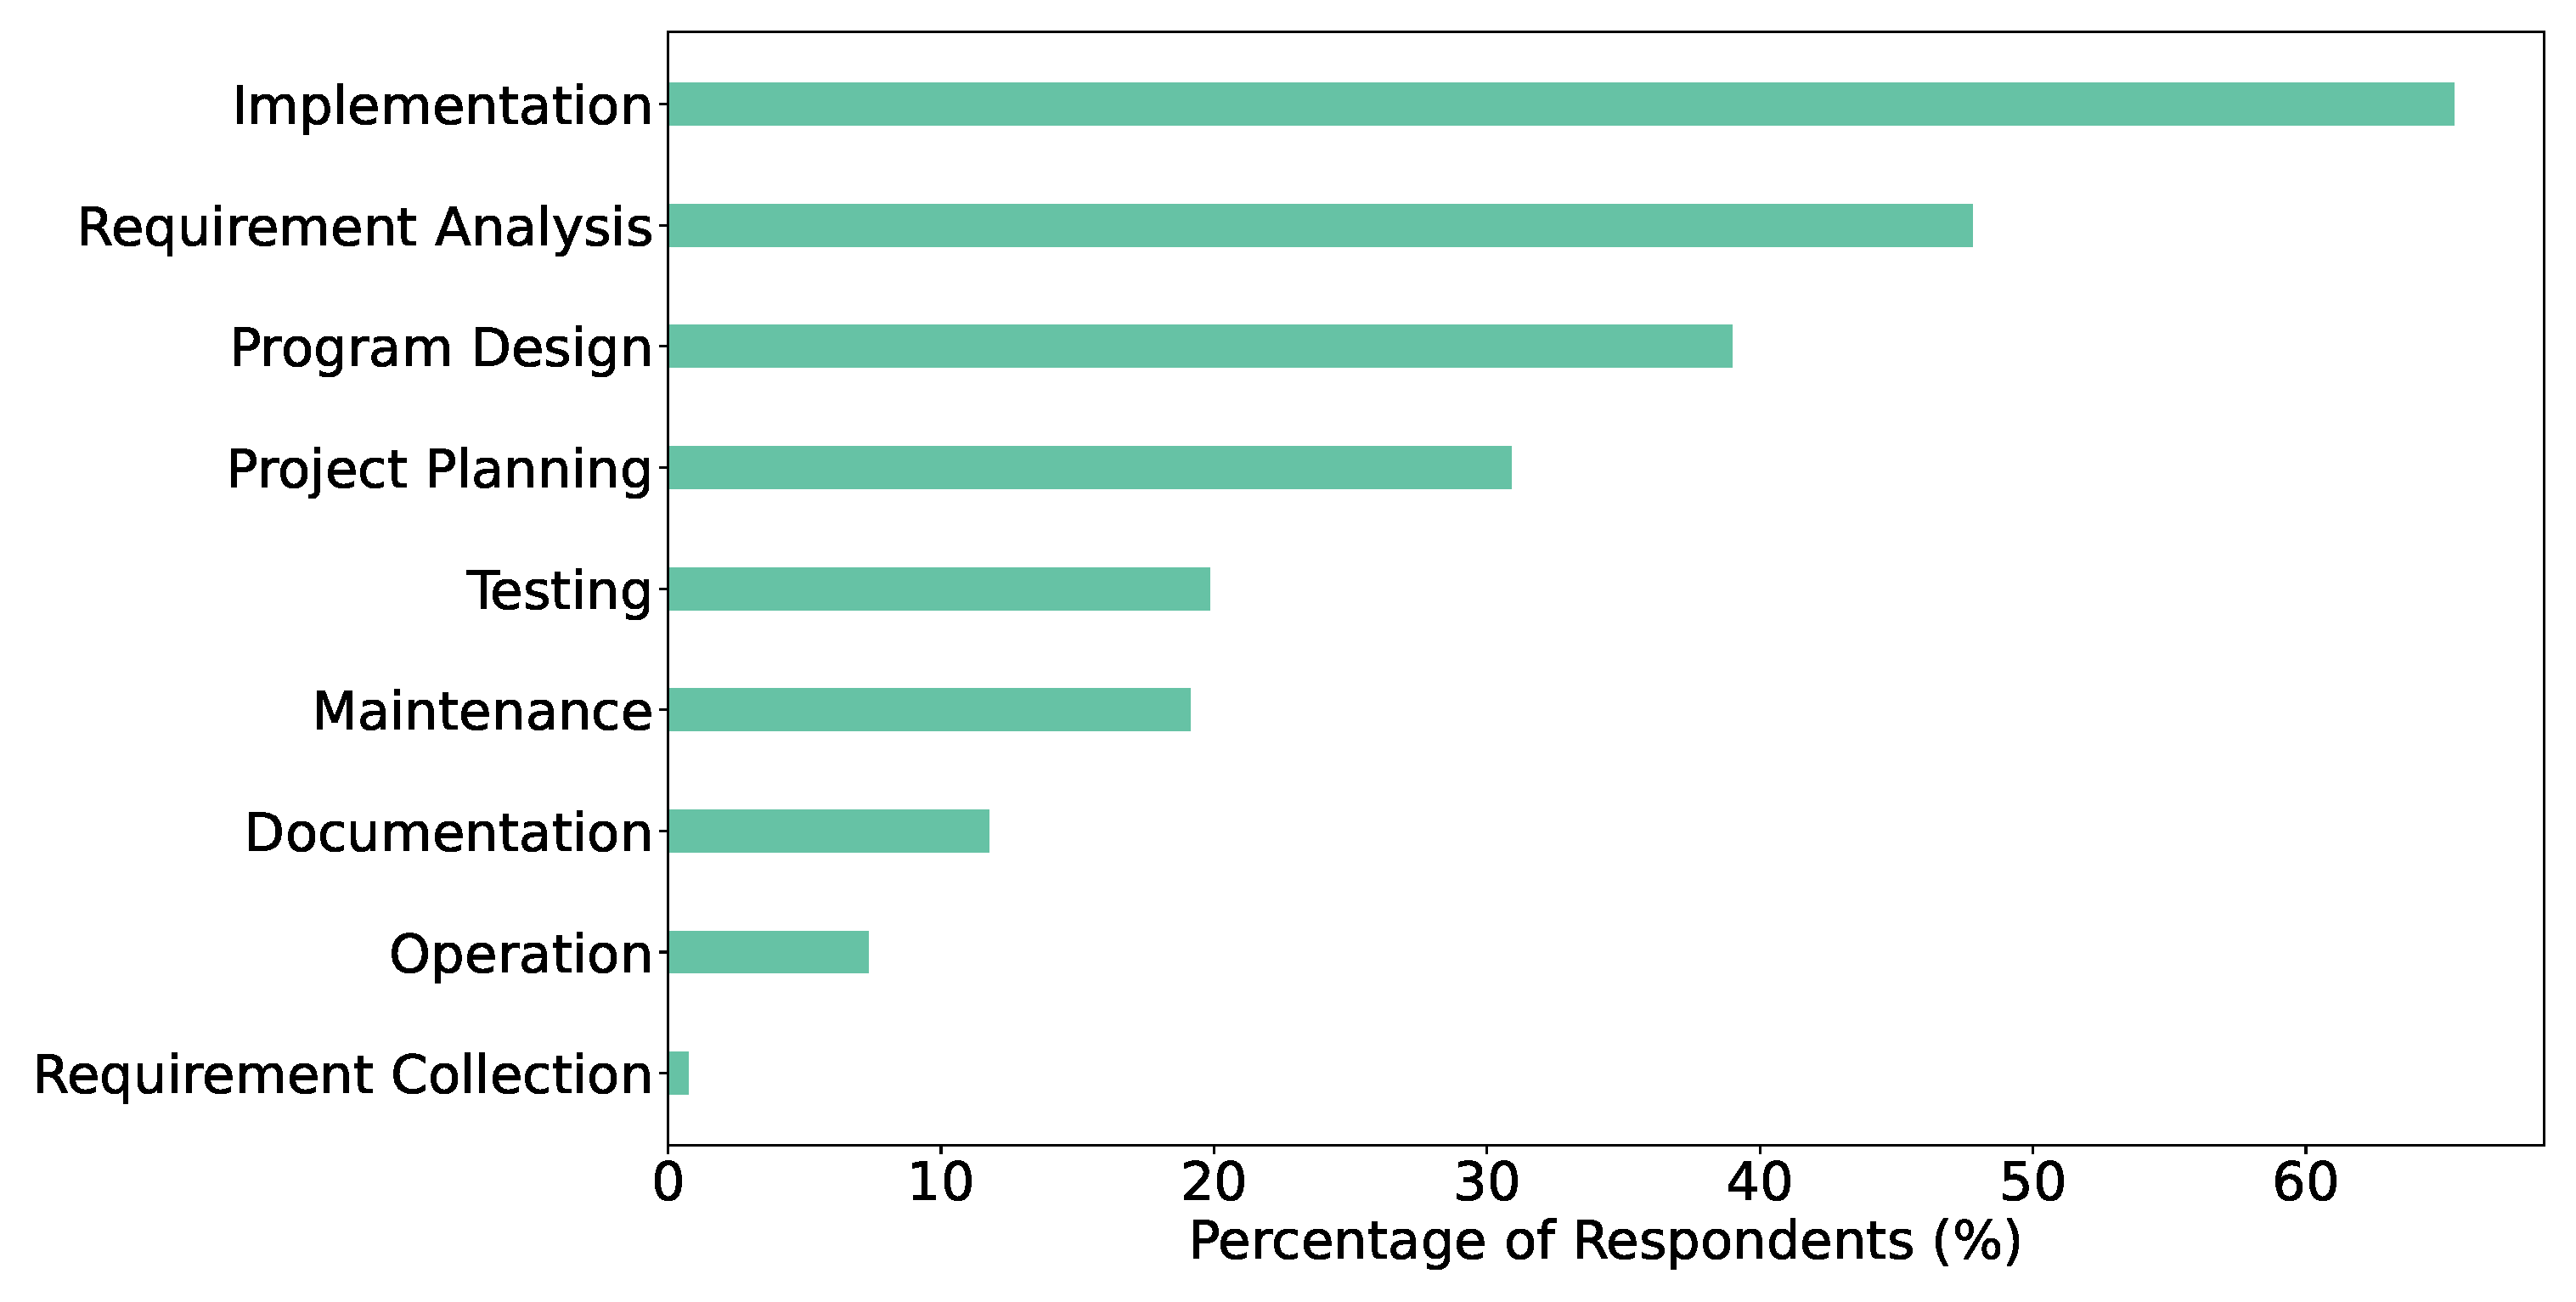
\includegraphics[width=0.8\textwidth]{Figures/Respondents_Activities}
%   \caption{Software development activities}
%   \label{fig:activities}
% \end{figure}


\subsubsection{Which implementation technologies and tools are adopted by software development professionals?}
\label{tools}

Our survey included five questions to find technologies and tools that are adopted by software development professionals. To answer this question fully, we report the following results:
\begin{itemize}
\item Technology Platform (Q 9).
\item Operating System (Q 10).
\item Programming Language (Q 11).
\item Framework (Q 12).
\item IDE (Q 13).
\end{itemize}

\paragraph{Technology Platforms}
Participants were allowed to choose multiple options. As shown in \ref{fig:platforms}, most of the respondents (80\%) worked in web platform. The rests were mobile (45\%), Desktop (30\%), Embedded/IOT (8\%).
% \begin{figure}[htbp]
% \centering
%   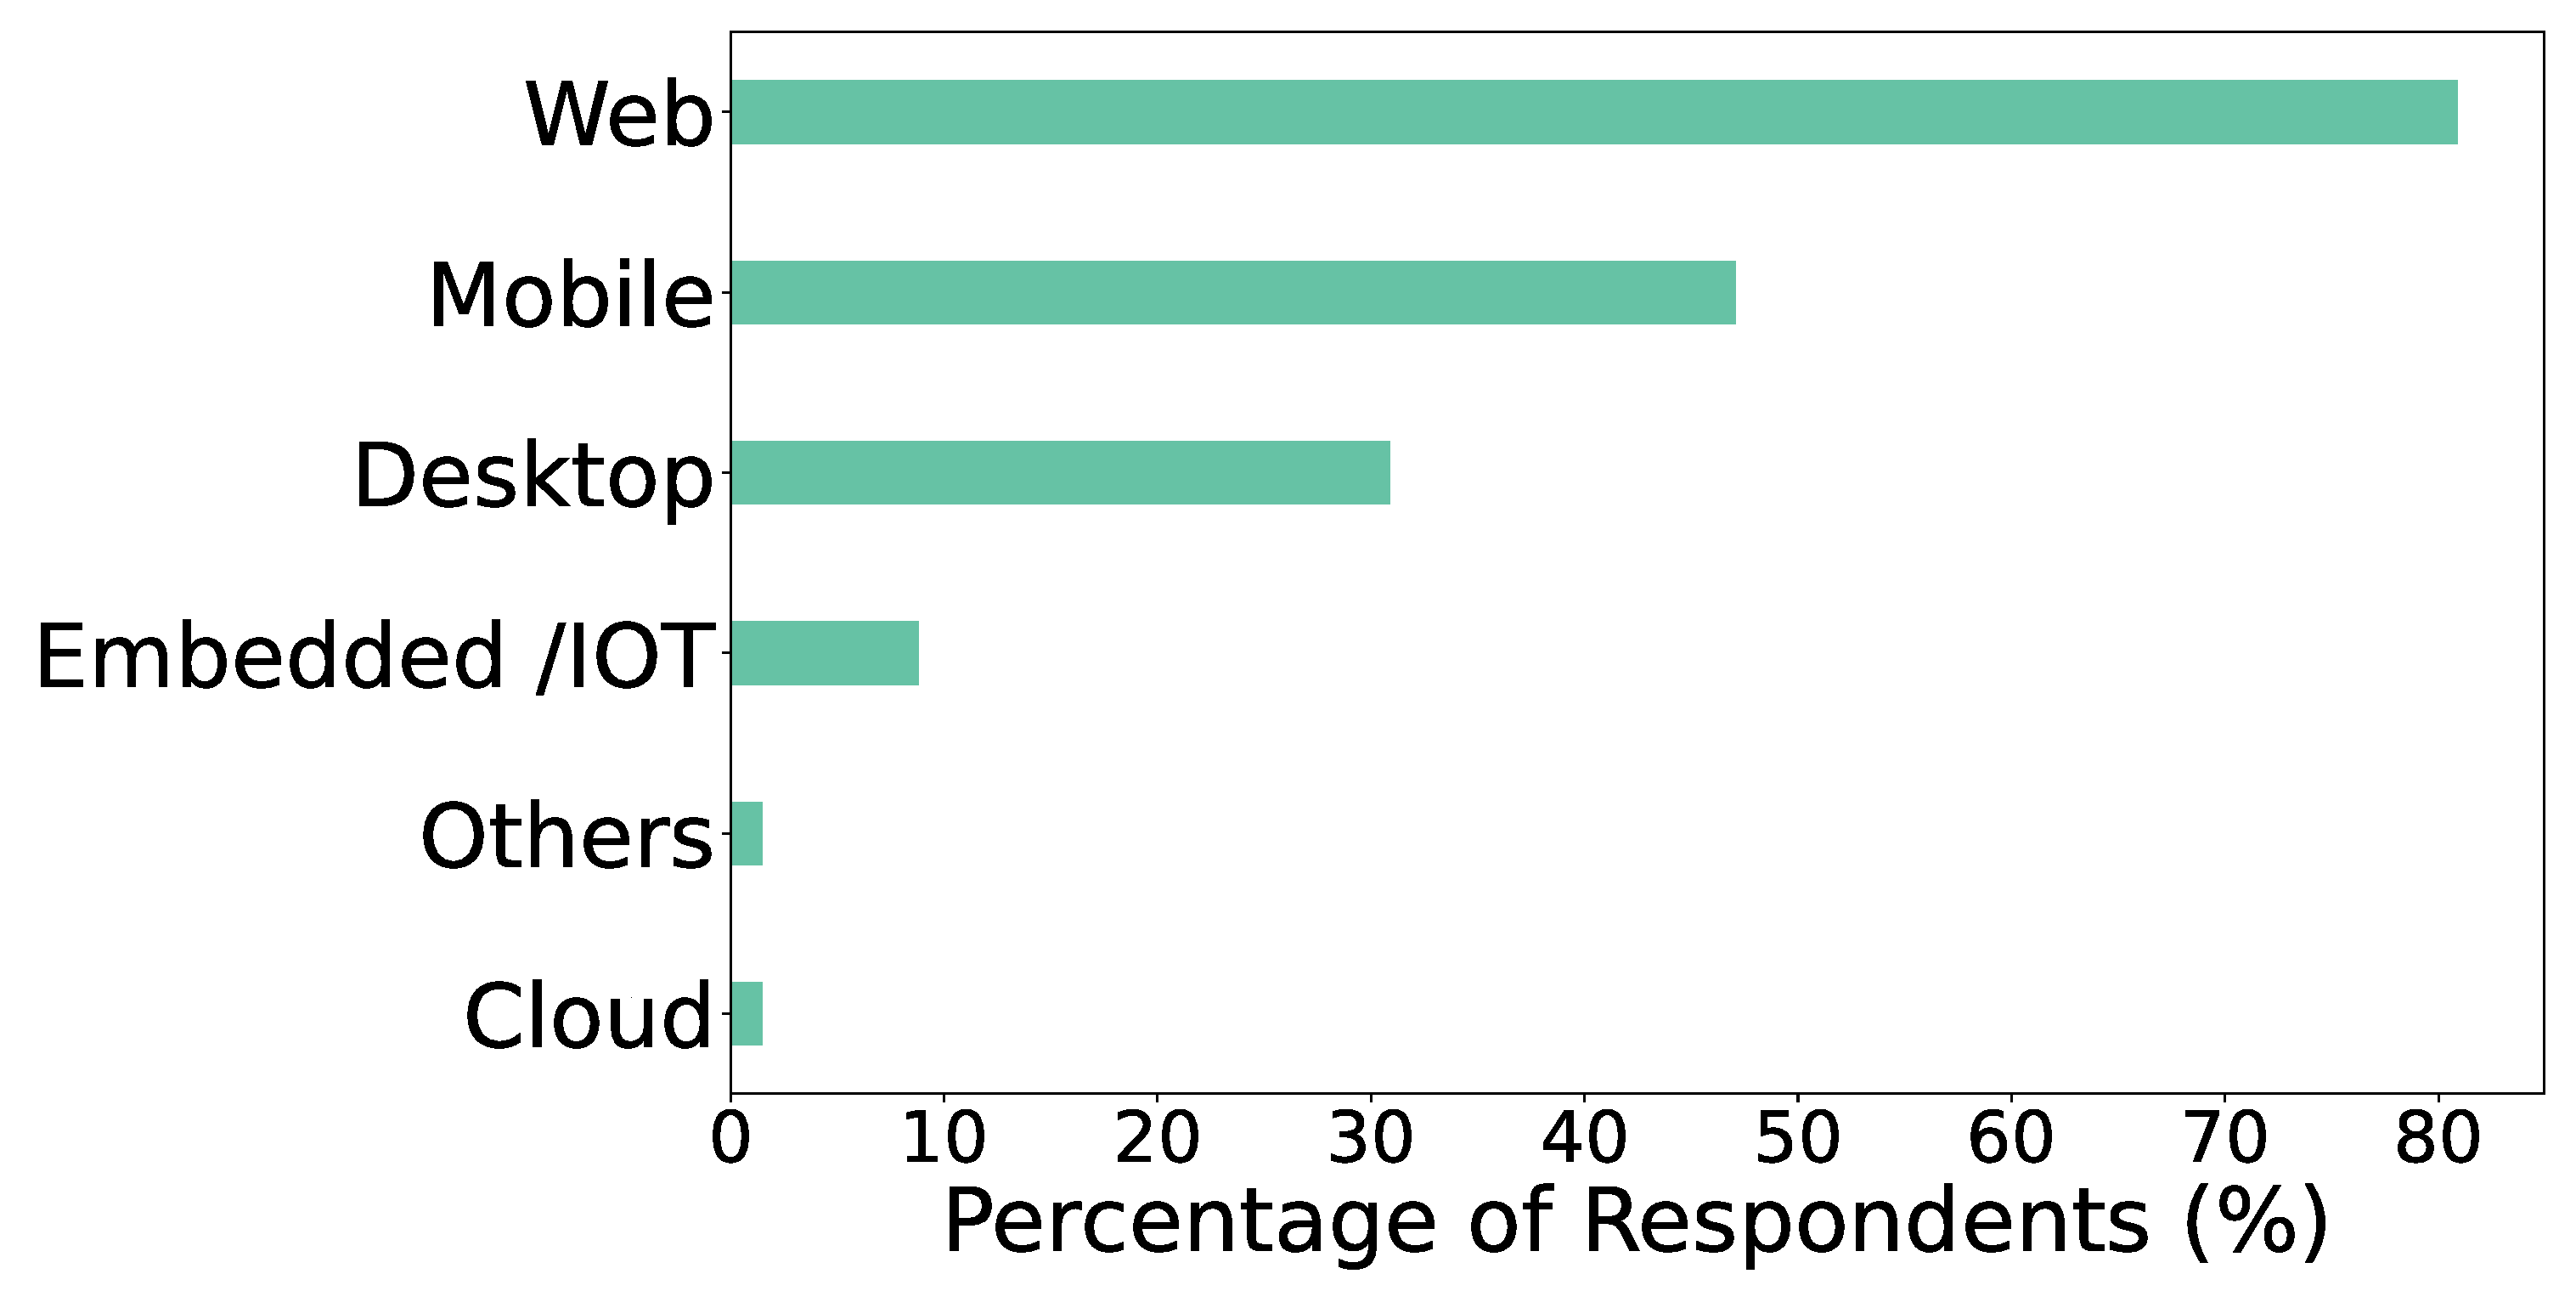
\includegraphics[width=0.8\textwidth]{Figures/Respondents_Technologies}
%   \caption{Technology Platforms}
%   \label{fig:platforms}
% \end{figure}

\paragraph{Operating Systems}
Most of our respondent's used linux based operating system (56\%). The second best used operating system is windows (45\%).

% \begin{figure}[htbp]
% \centering
%   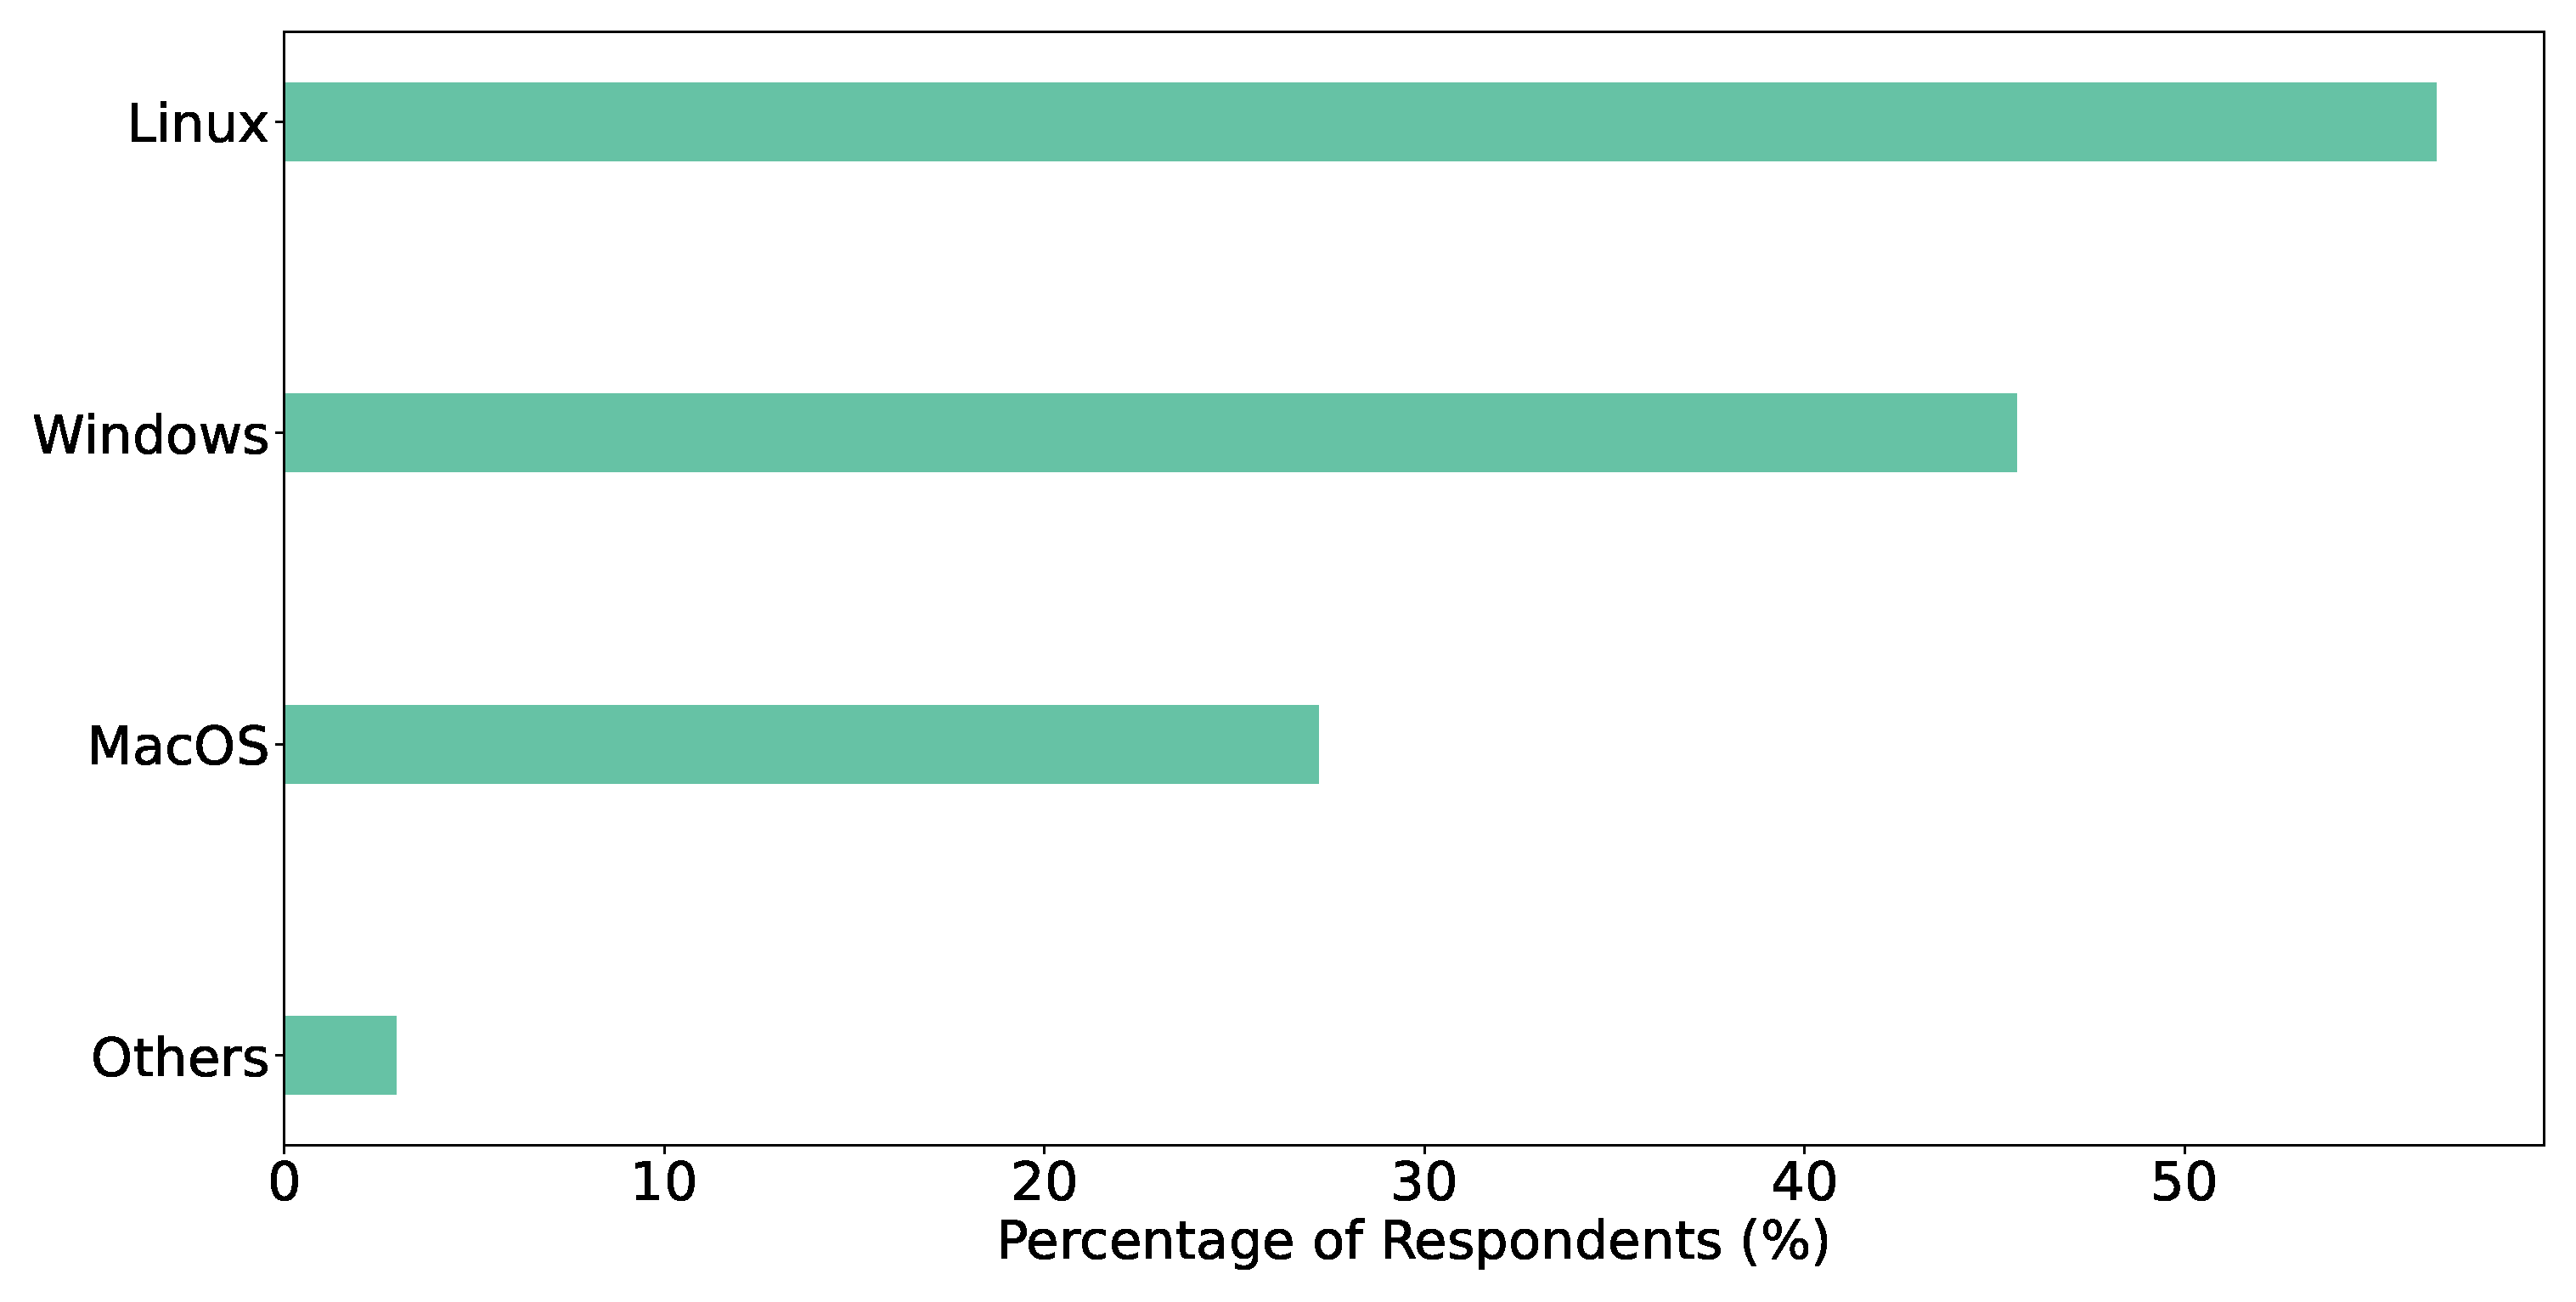
\includegraphics[width=0.8\textwidth]{Figures/Respondents_os}
%   \caption{Operating Systems}
%   \label{fig:os}
% \end{figure}

\paragraph{Programming Languages}
According to \ref{fig:languages}, around 61\% of our respondent's used Java and Javascript each. Other languages like php (25\%), python (25\%), c\# (18\%) are also used which indicates that the software engineers are not inclined towards a single specific language. Also the choice of programming languages used for development can have important inferences for the testing practices of a software company.

% \begin{figure}[htbp]
% \centering
%   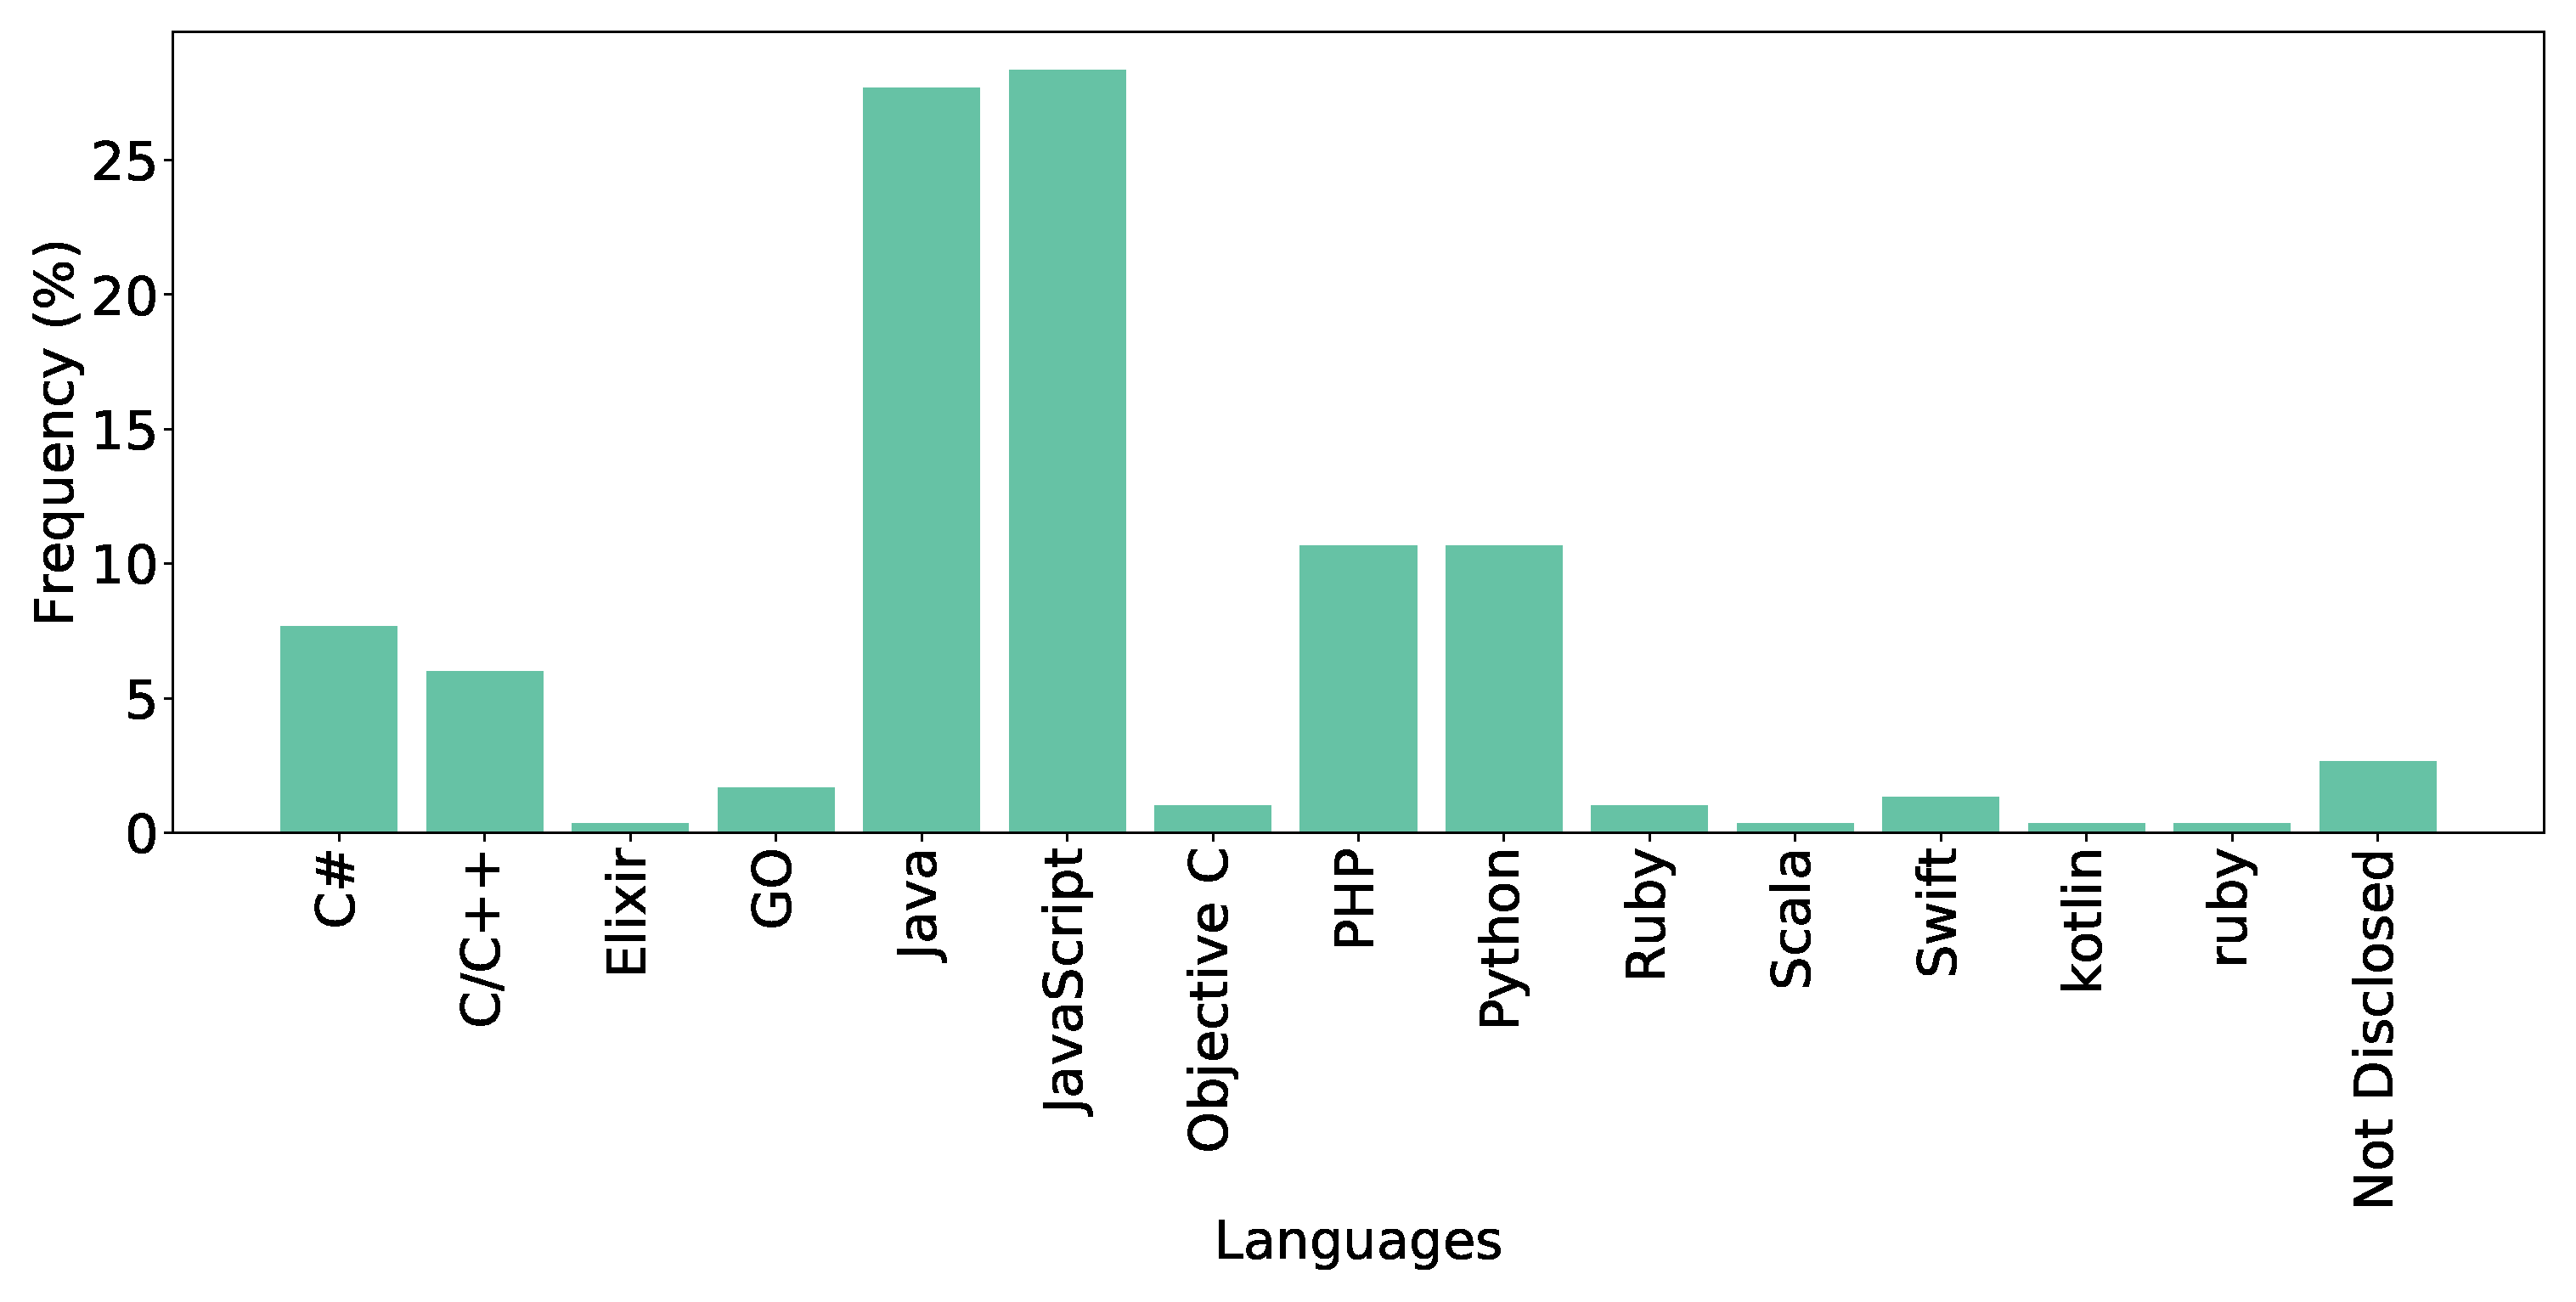
\includegraphics[width=0.8\textwidth]{Figures/Respondents_languages}
%   \caption{Languages used in software development}
%   \label{fig:languages}
% \end{figure}

\paragraph{Frameworks used in development}
As shown in \ref{fig:frameworks}, variety of frameworks have been used during development. Spring boot (37\%) is the mostly used framework in the industry. ASP.NET, Django and Laravel are used in same proportion (14\%).
% \begin{figure}[htbp]
% \centering
%   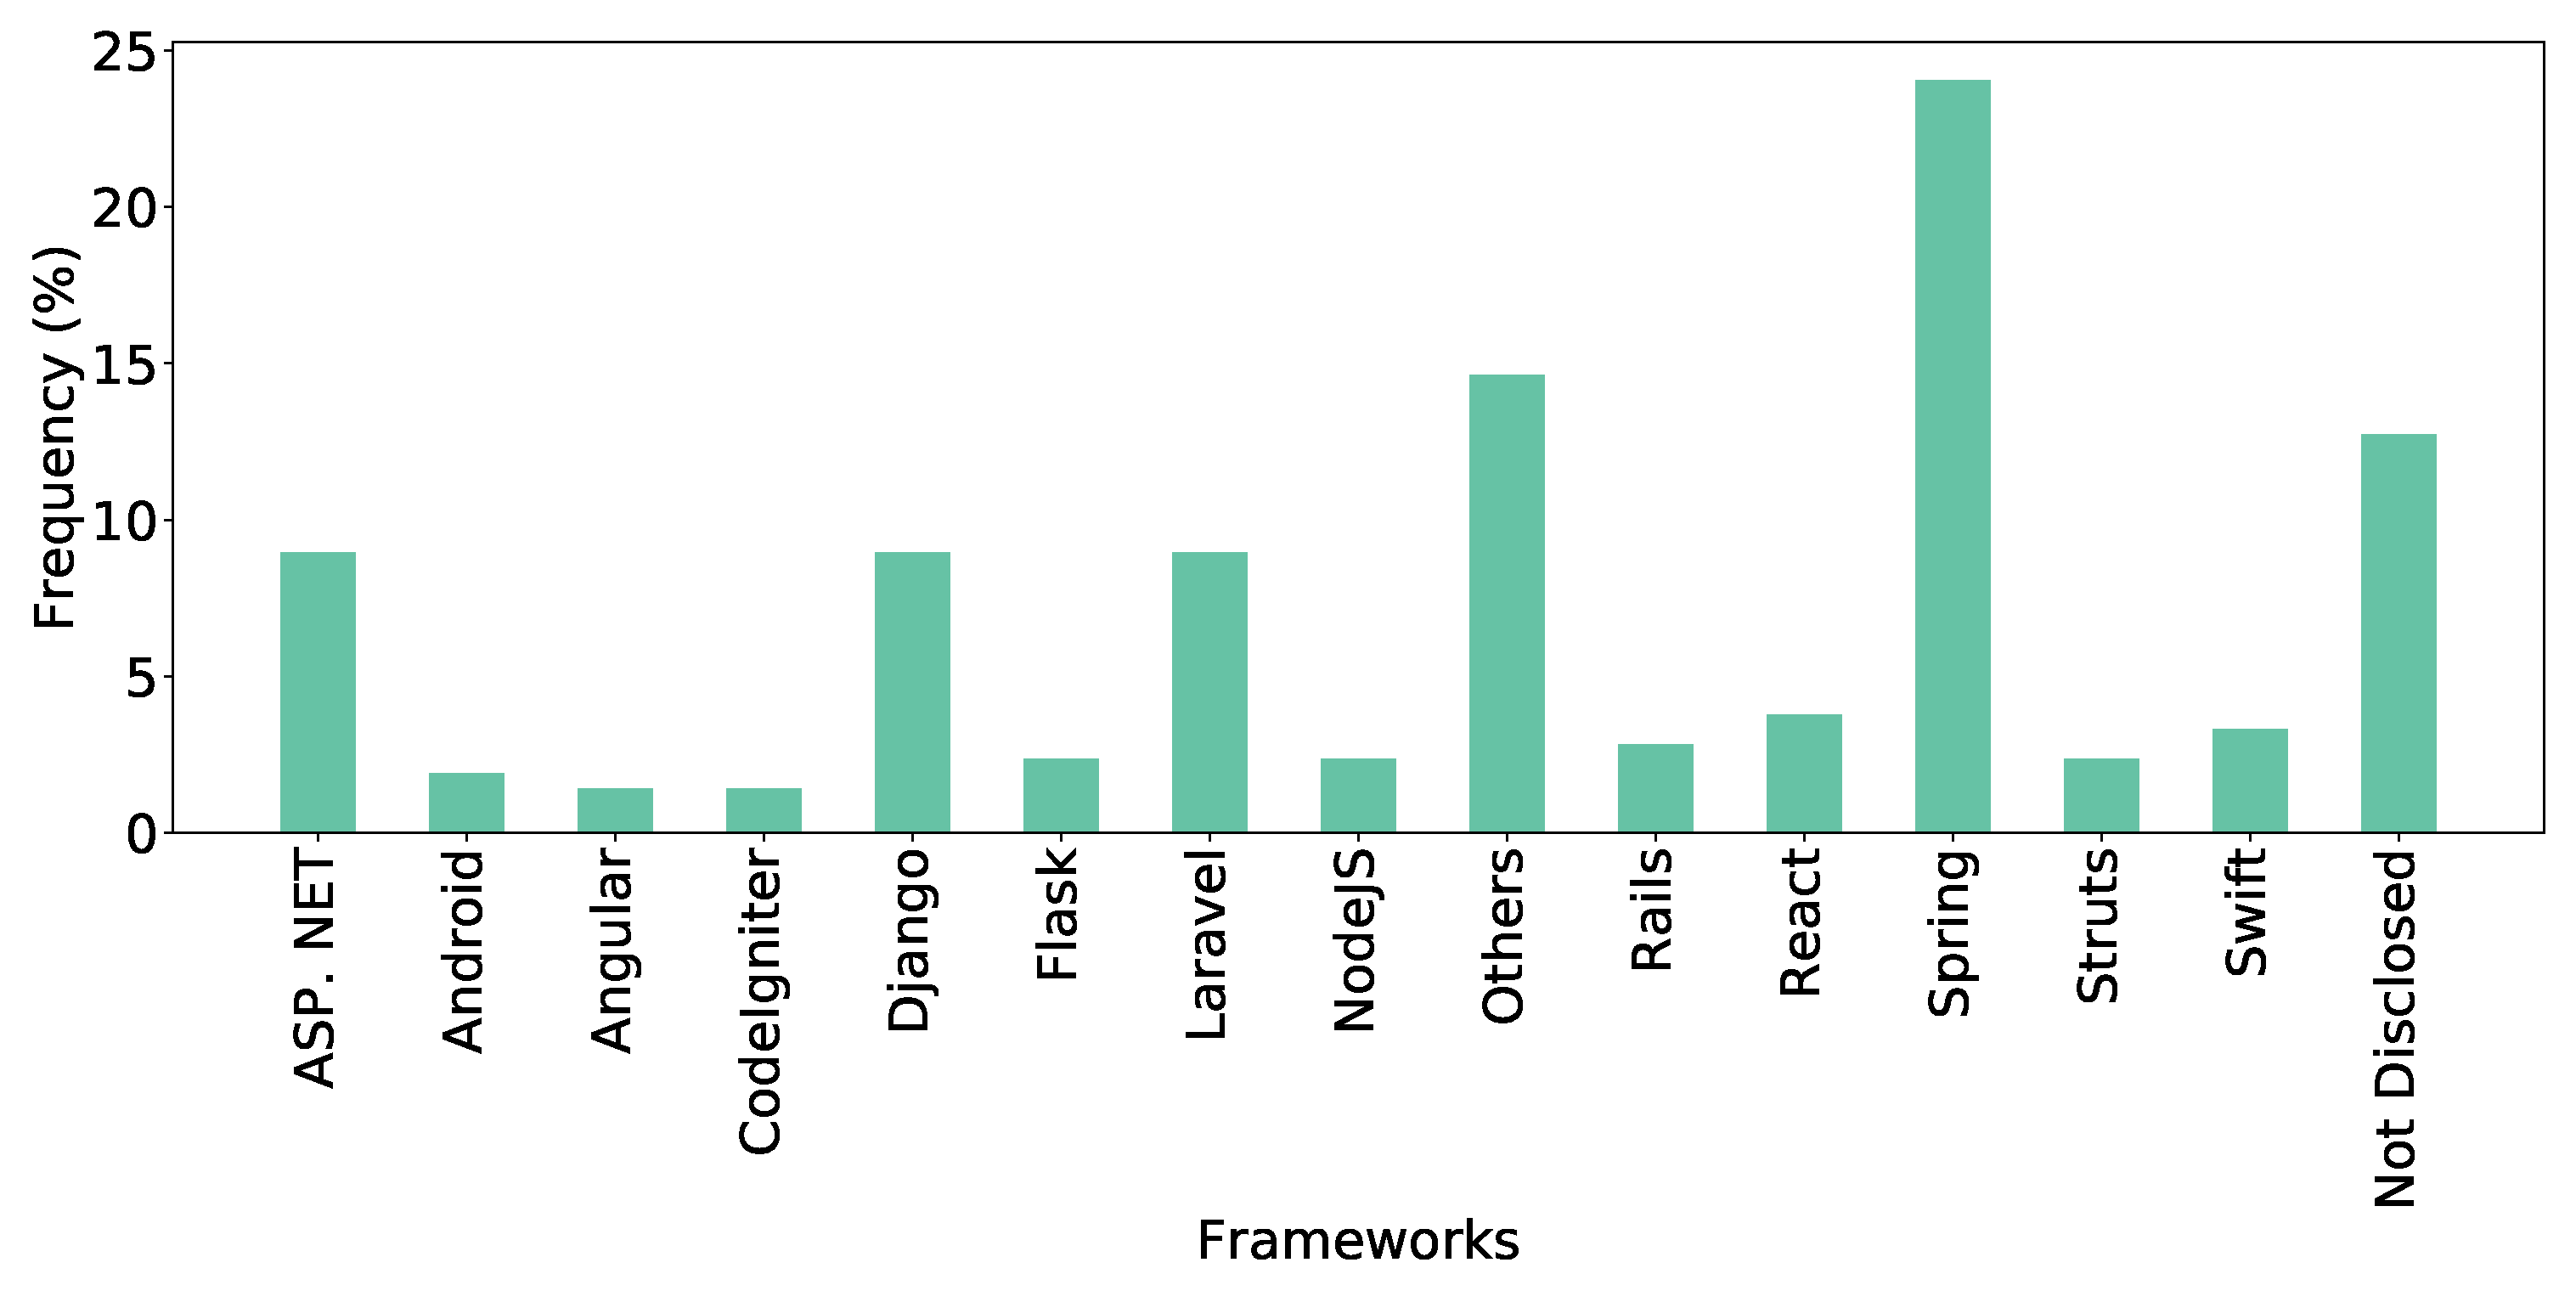
\includegraphics[width=0.8\textwidth]{Figures/Respondents_frameworks}
%   \caption{Frameworks}
%   \label{fig:frameworks}
% \end{figure}

\paragraph{IDE's used by the respondent's}
According to \ref{fig:IDEs}, IntelliJ, a Java integrated development environment for developing computer software for enterprise, mobile, and web development used by most of the respondents (43\%). The other IDEs used in SE industries are: visual studio (30\%), Eclipse (24\%), PyCharm (16\%), NetBeans (10\%), Android Studio (6\%).
% \begin{figure}[htbp]
% \centering
%   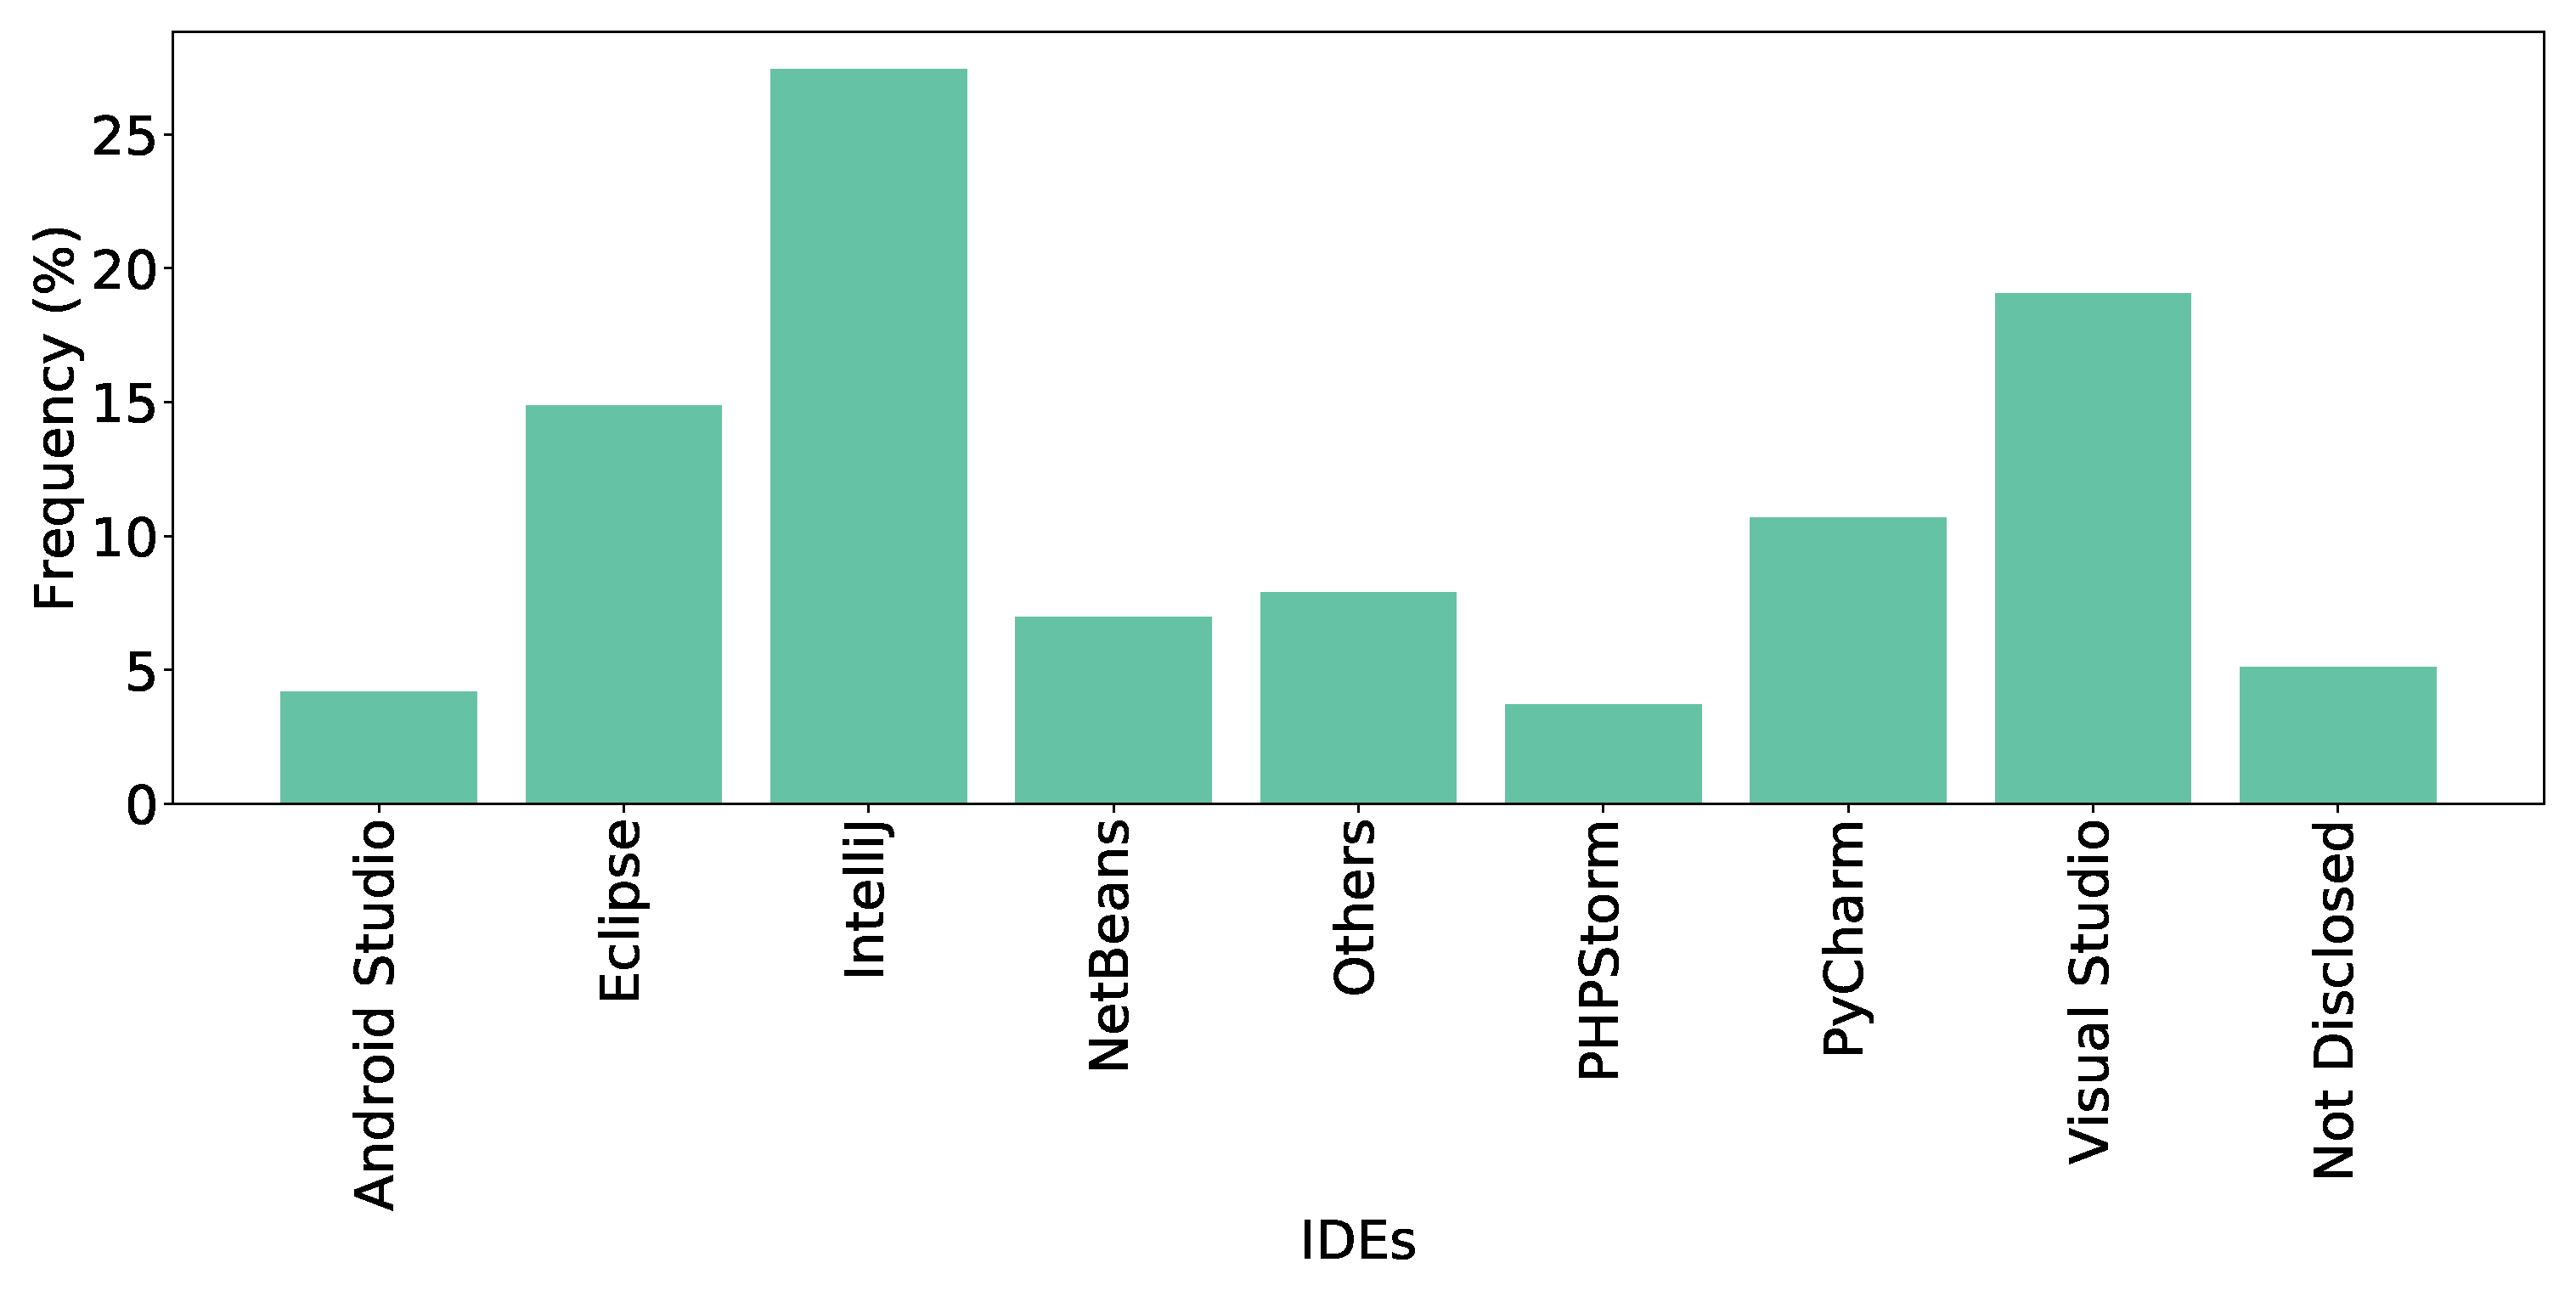
\includegraphics[width=0.8\textwidth]{Figures/Respondents_IDEs}
%   \caption{IDE's}
%   \label{fig:IDEs}
% \end{figure}

\subsubsection{What type of testing and deployment practices are used?}
\label{testing_practices}

Testing is an important process in improving the quality of the software product. The purpose of this process is to find errors, which might occur during specification, design and code generation. Here we report the following results next:
\begin{itemize}
\item Software Testing Practices (Q 14)
\item Level of Automated Testing (Q 15)
\item Tools Used in Testing and QA (Q 16)
\item Continuous Deployment tools (Q 17)
\item Version Control (Q 18)
\end{itemize}


\paragraph{Software Testing Practices}
According to \ref{fig:testing}, several number of testing practices are used during software development. The results show most of the organizations carried out unit testing (53\%), functional testing (49\%), user acceptance testing (39\%), GUI testing (31\%) etc.

% \begin{figure}[htbp]
% \centering
%   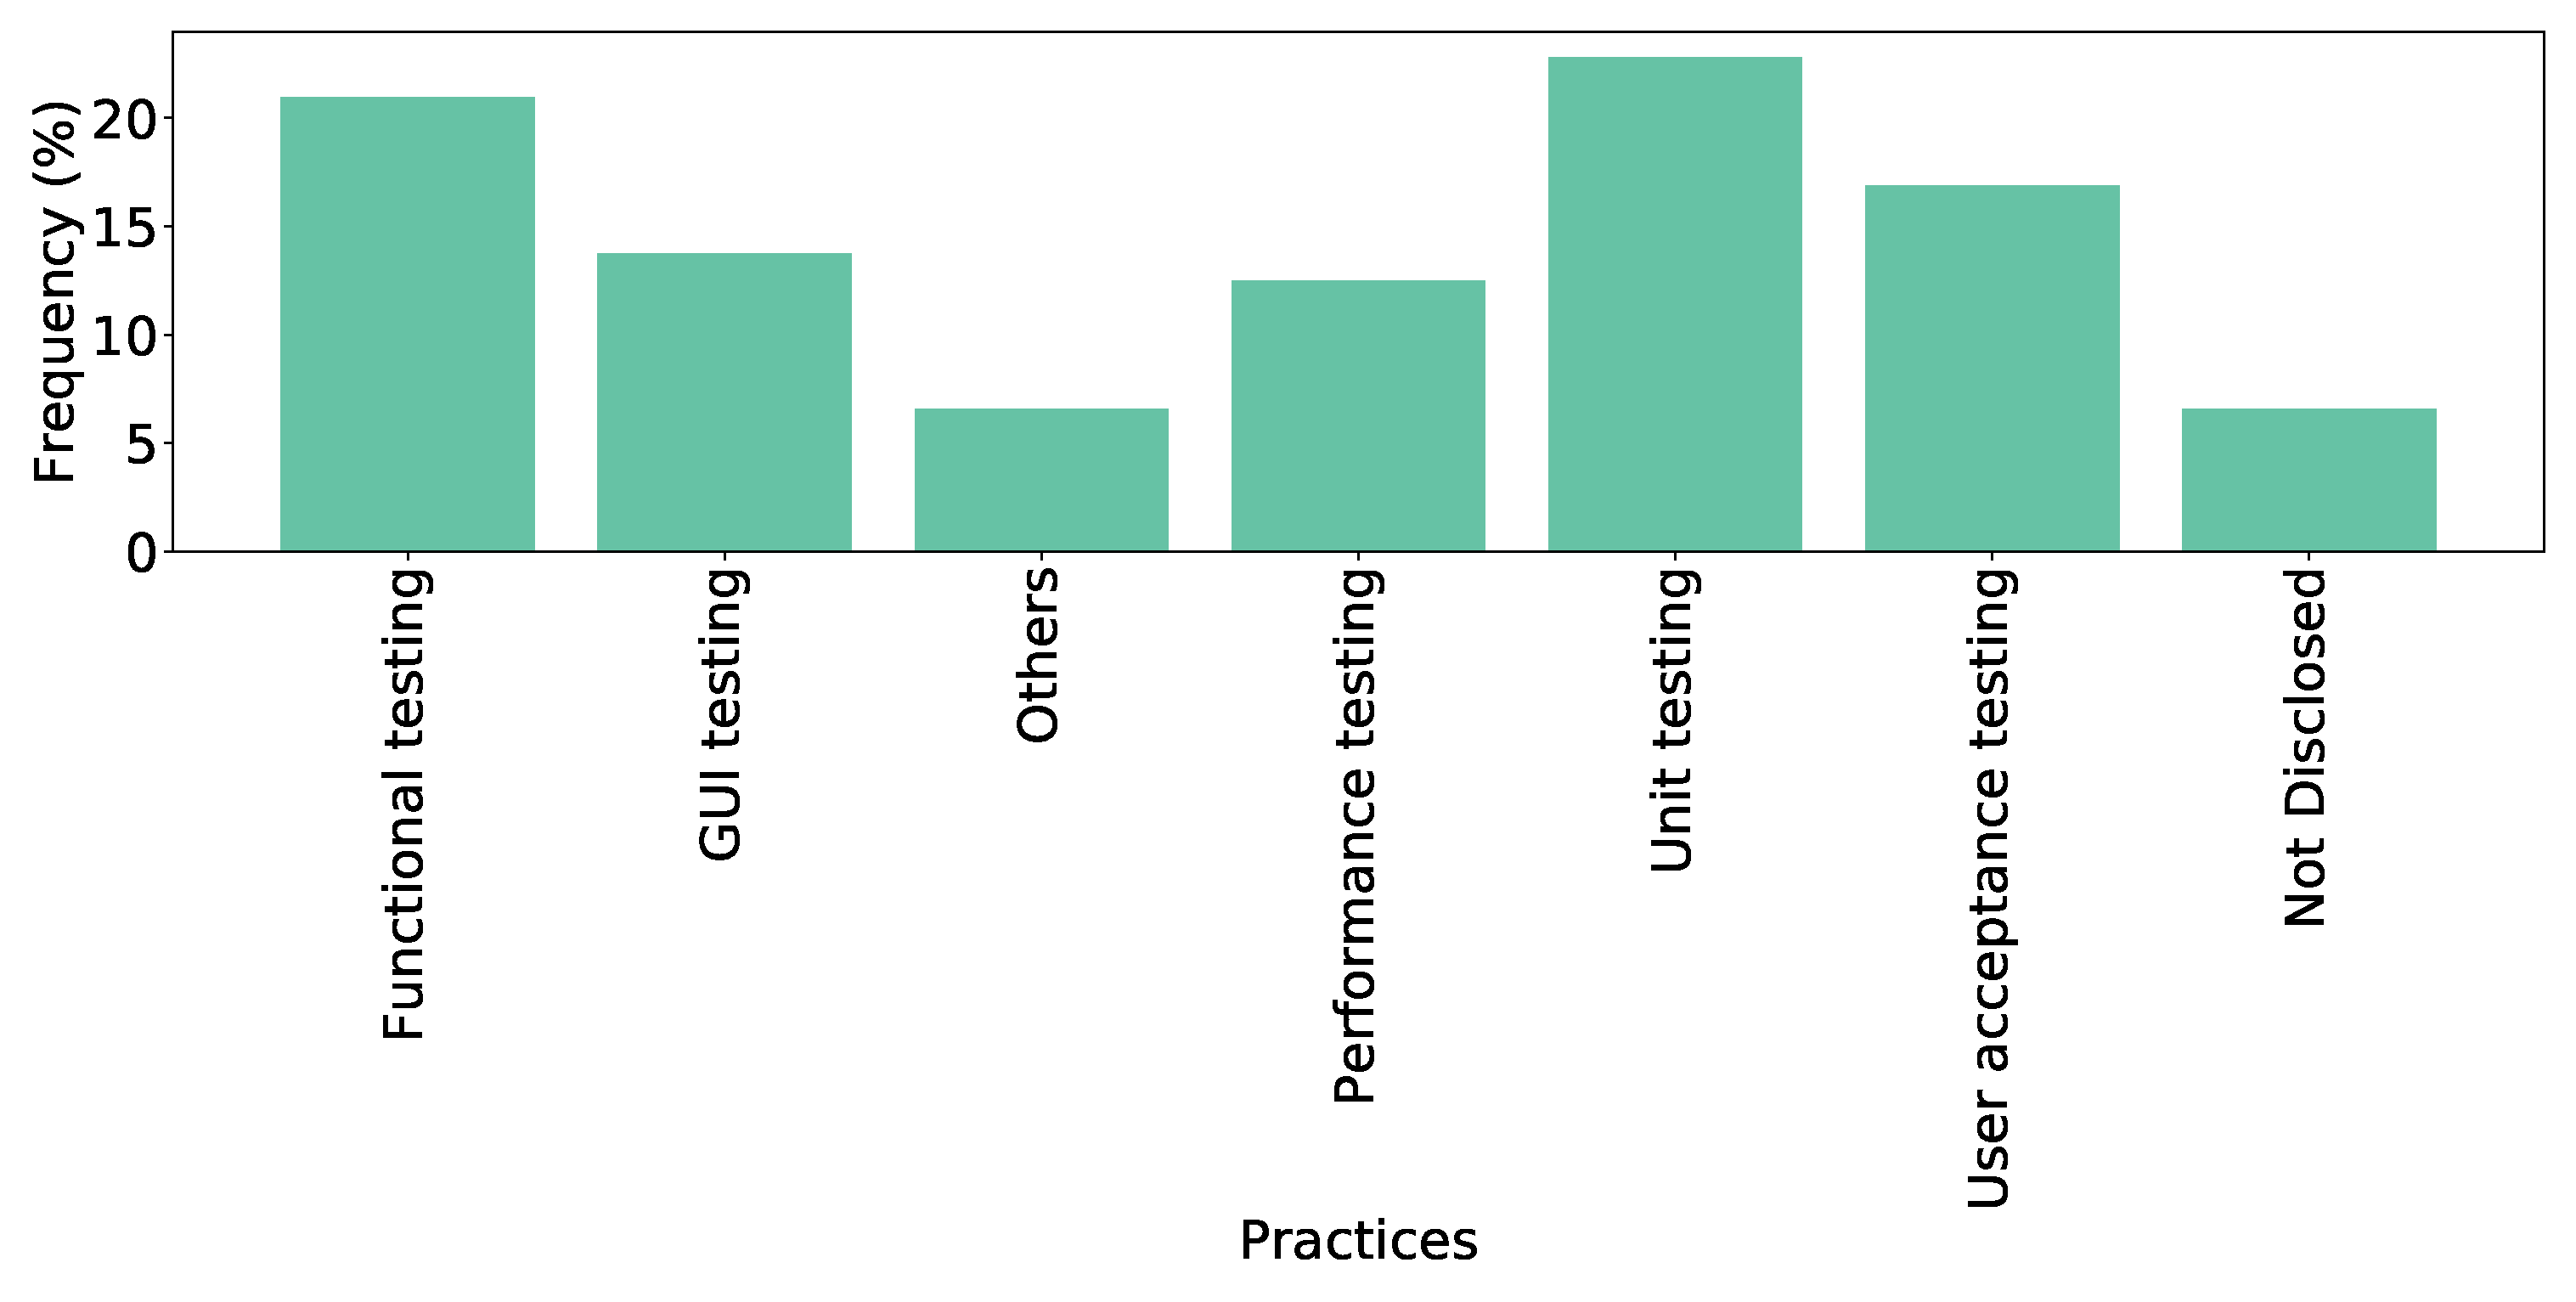
\includegraphics[width=0.8\textwidth]{Figures/Respondents_testing_practices}
%   \caption{Testing Practices}
%   \label{fig:testing}
% \end{figure}


\paragraph{Level of Automated Testing}
Question 15 asked about the level of automated testing. The responses were gathered using the Likert scale. This denotes that different respondents have very different practices in this context, i.e., some heavily practice automated testing, while others favor manual testing. Results are shown in \ref{fig:autoTest}.

% \begin{figure}[htbp]
% \centering
%   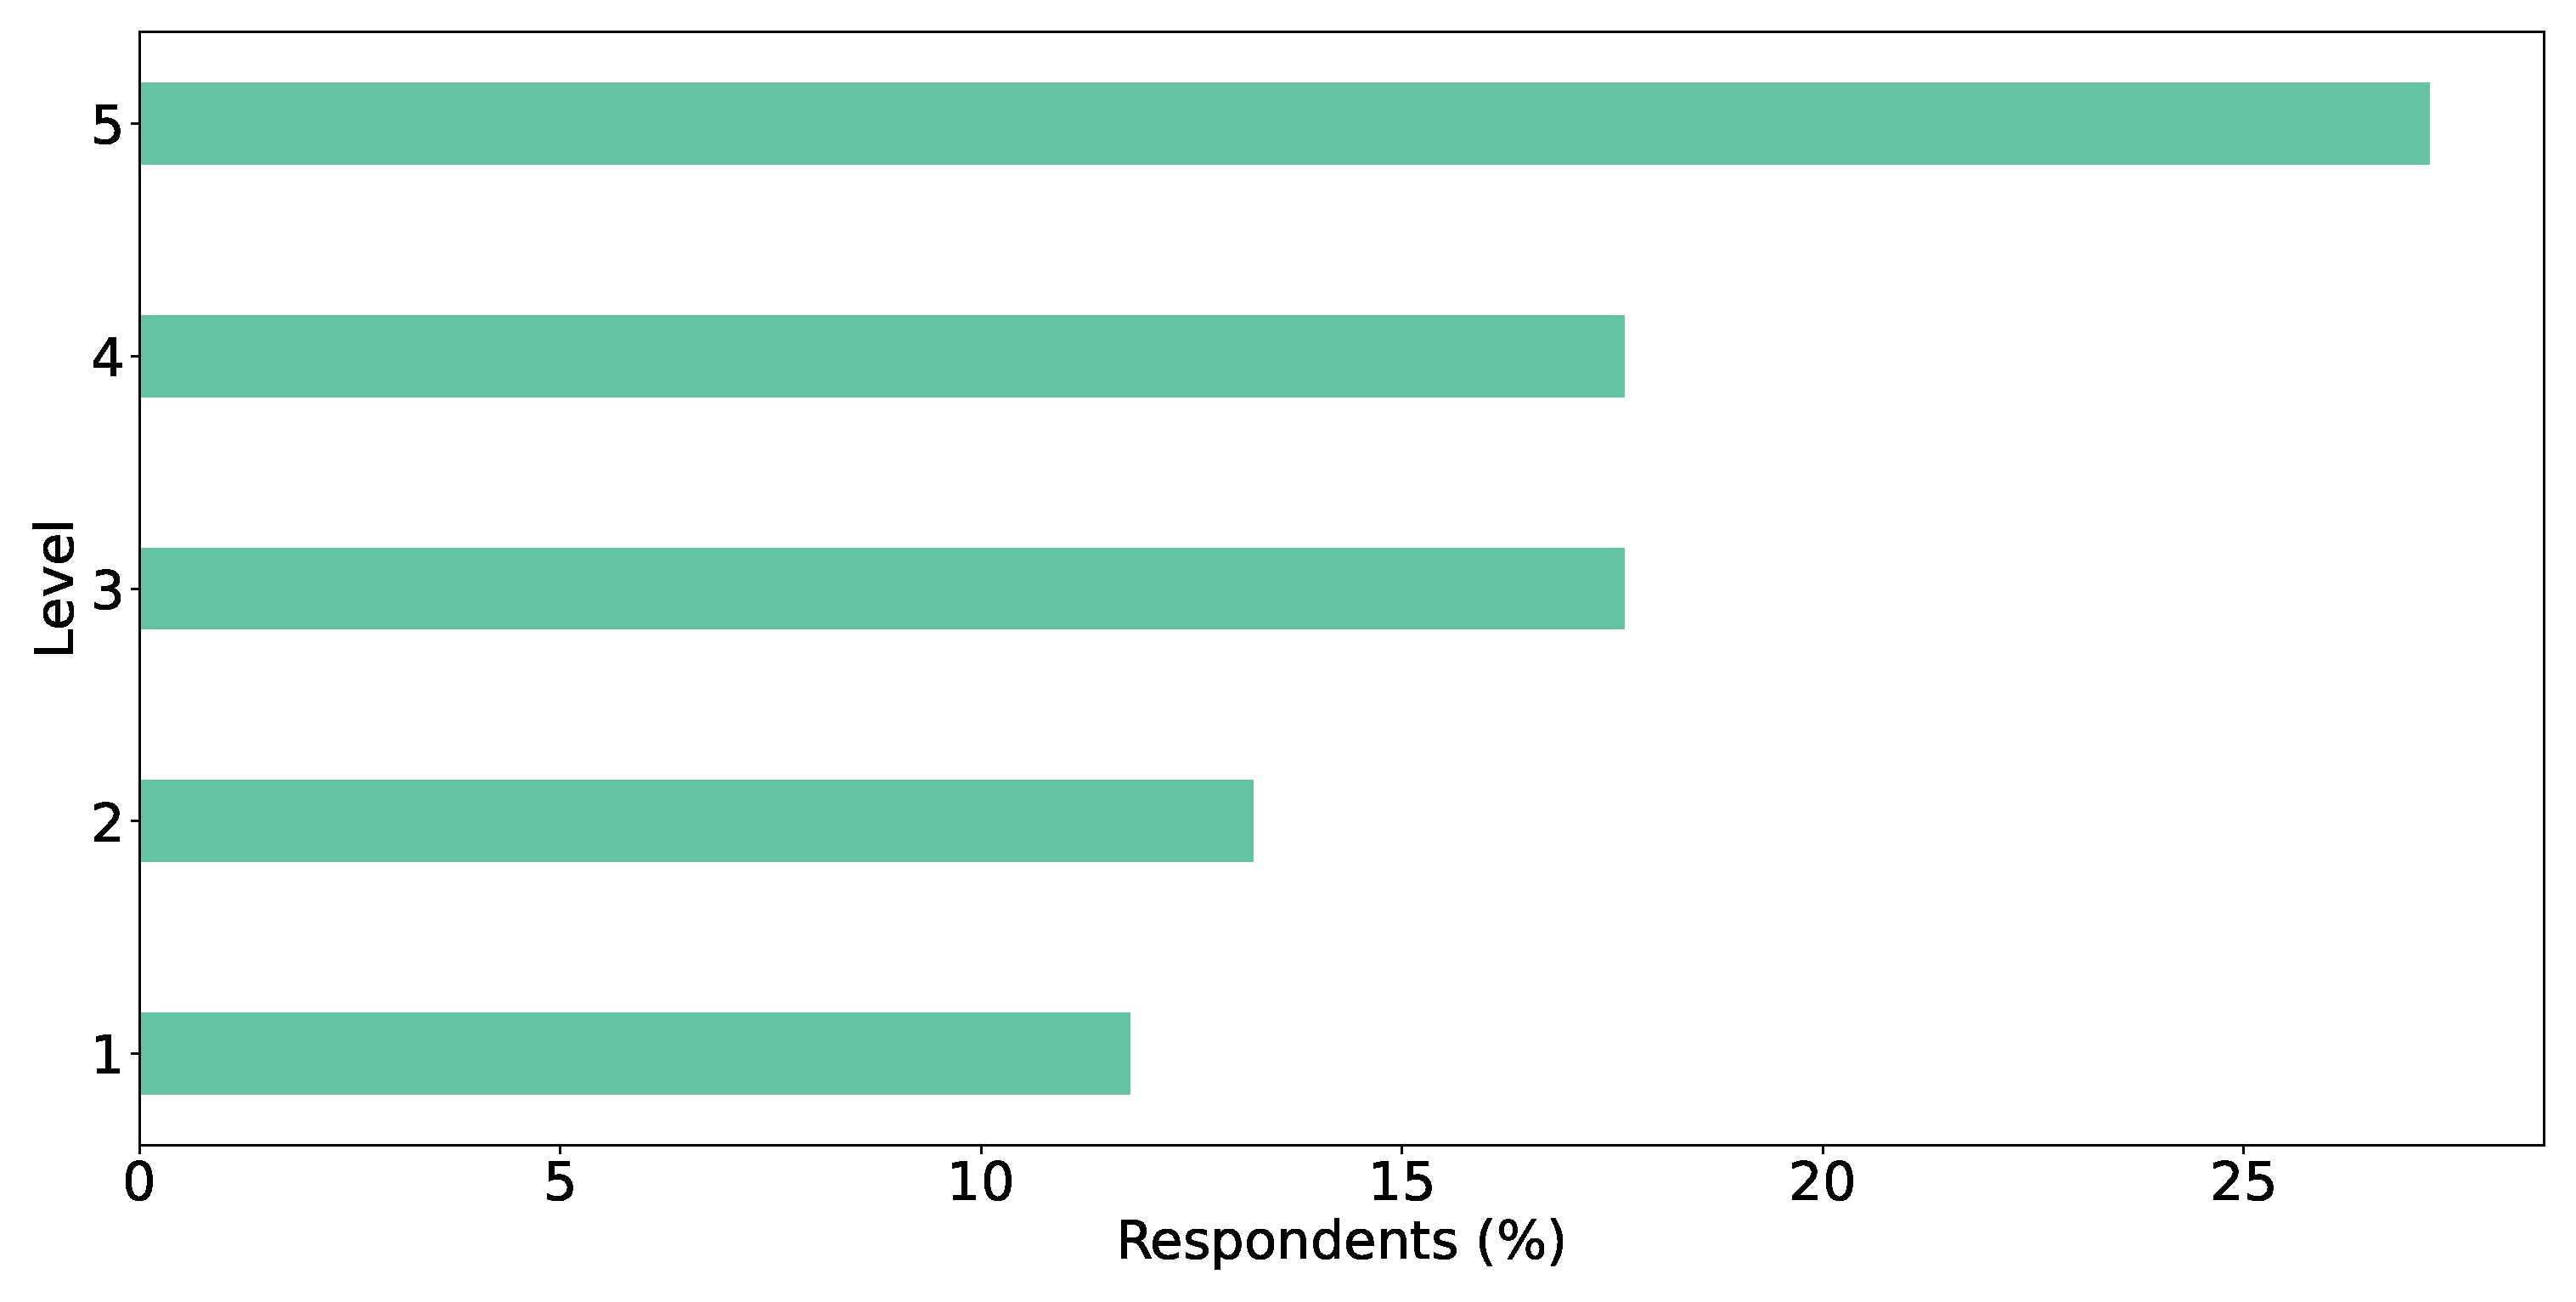
\includegraphics[width=0.8\textwidth]{Figures/Respondents_autotest_level}
%   \caption{Automated Testing Level}
%   \label{fig:autoTest}
% \end{figure}


\paragraph{Tools Used in Testing and QA}
Q 16 asked about the tools used in testing and quality assurance. According to \ref{fig:testingTools}, we see that most of the respondents have been used XUnit( eg, JUnit, NUnit) (30\%), selenium (27\%), Jenkins (20\%), others (9\%).

% \begin{figure}[htbp]
% \centering
%   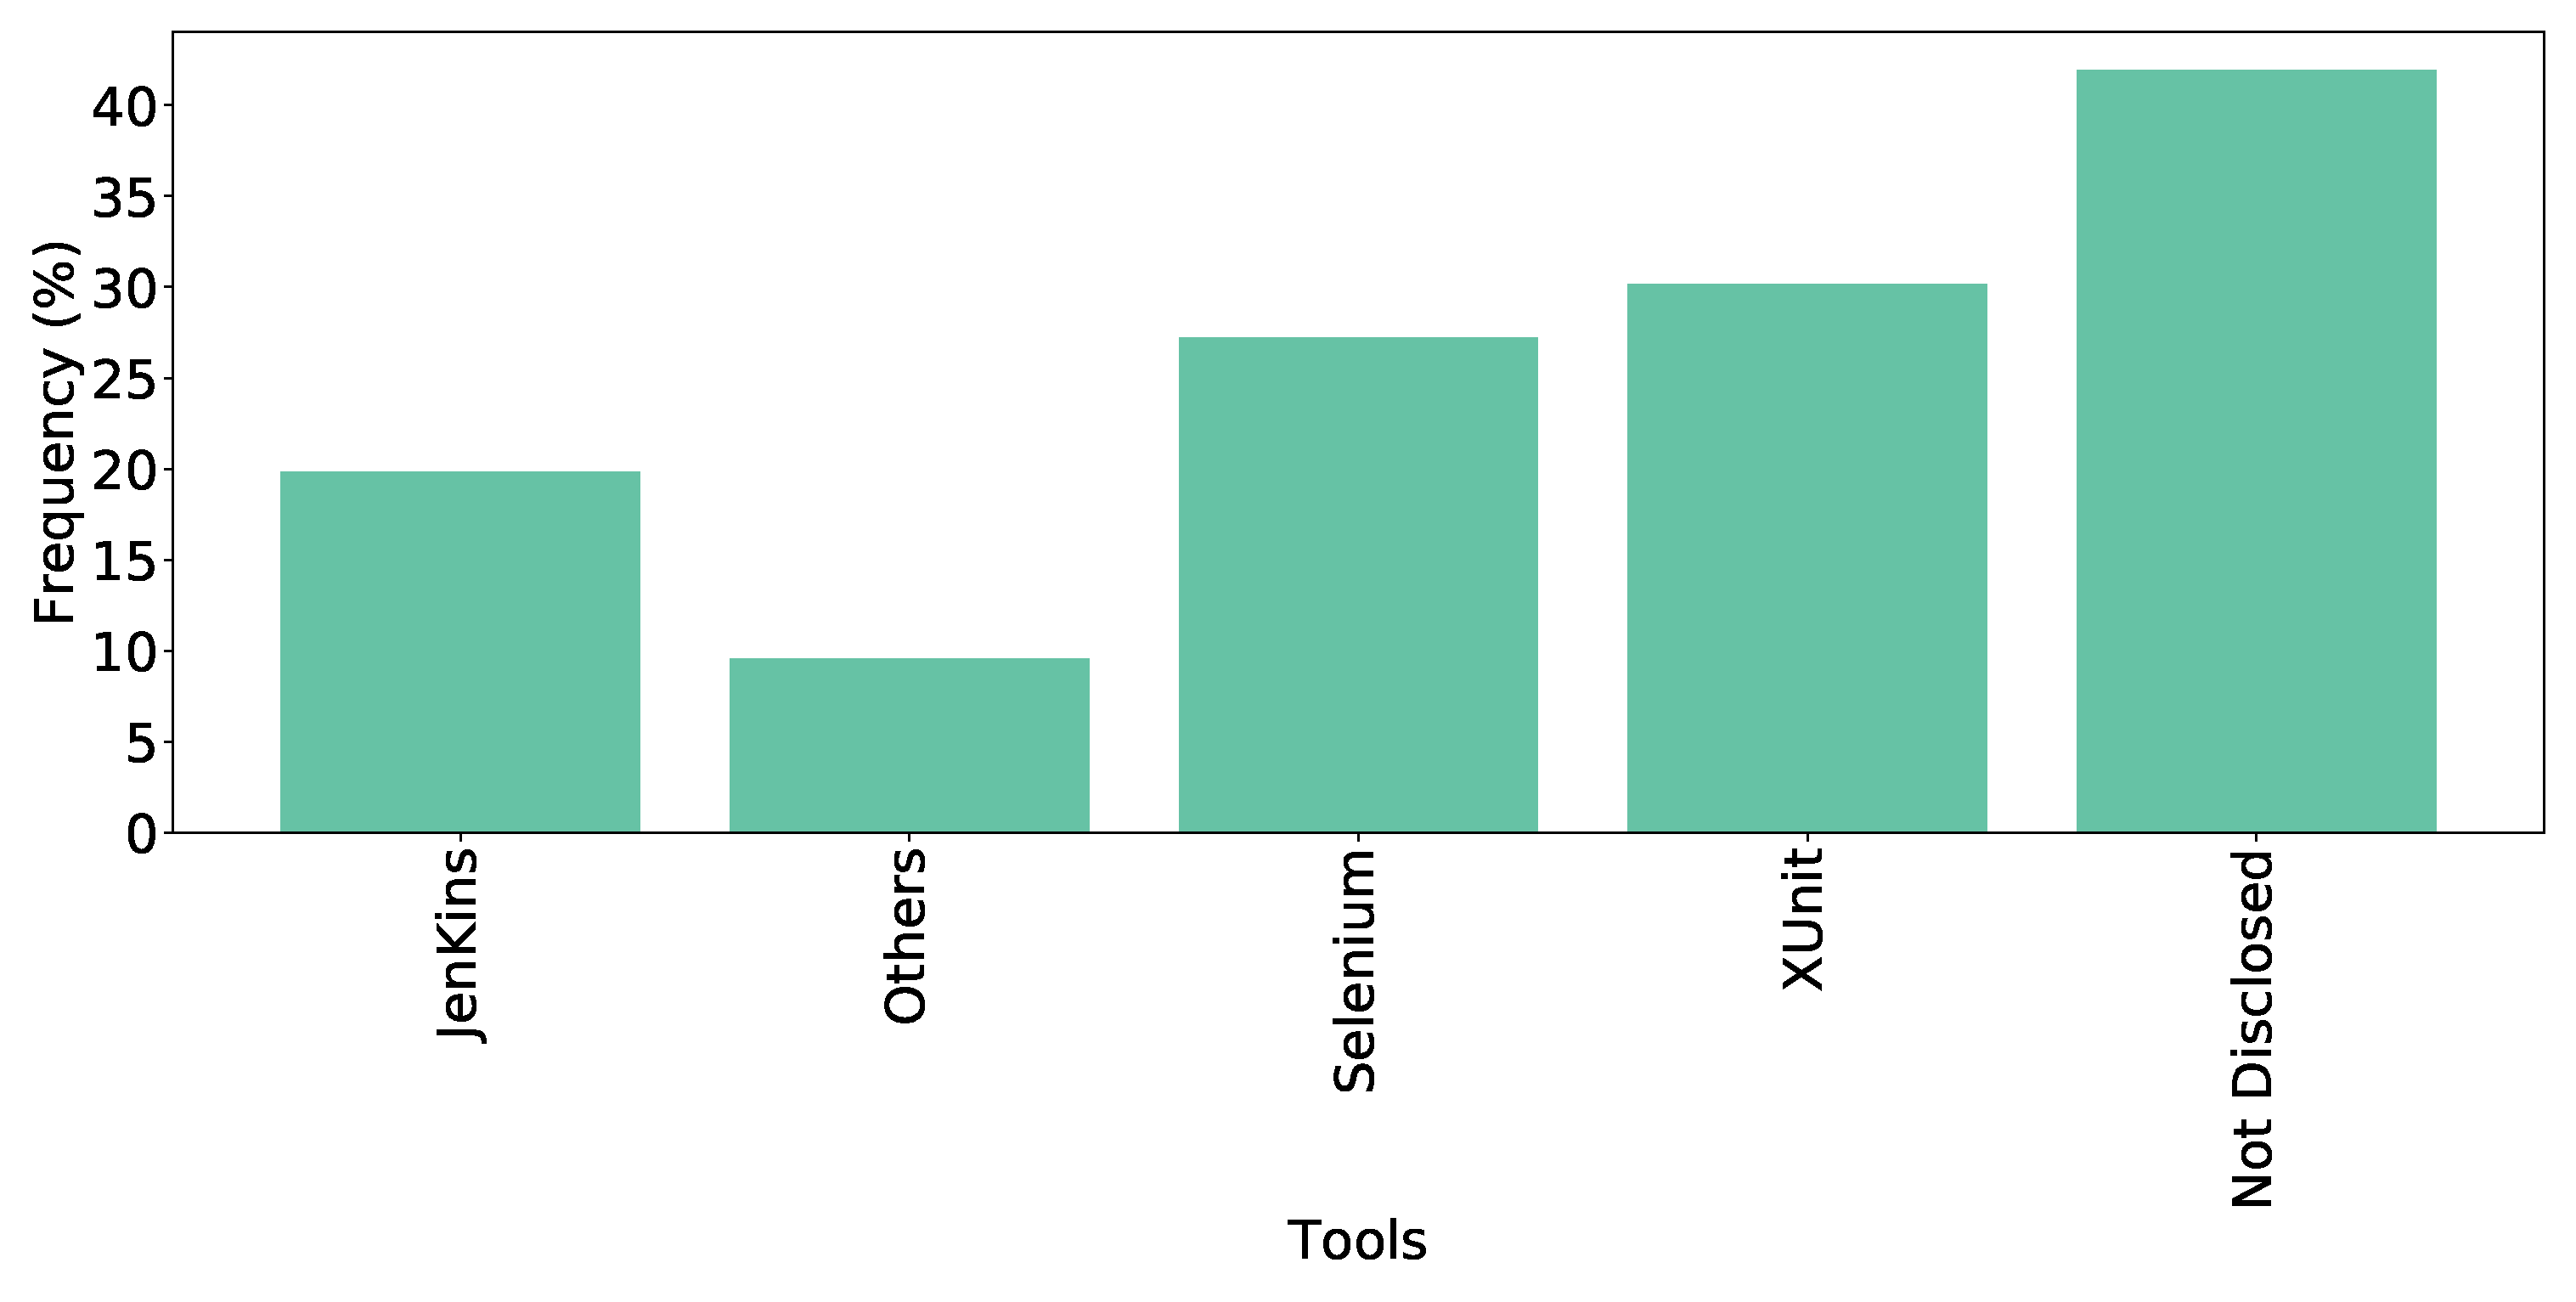
\includegraphics[width=0.8\textwidth]{Figures/Respondents_testing_tools}
%   \caption{Testing \& QA Tools}
%   \label{fig:testingTools}
% \end{figure}


\paragraph{Deployment Tools}
According to \ref{fig:deployTools}, wee see that most of the respondents use AWS code-deploy (12\%) and JenKins (12\%). The other deployment tools are Bamboo (5\%), teamcity (4\%), octopus (2\%). Respondents voted none (4\%) as they didn’t use any deployment tools.

% \begin{figure}[htbp]
% \centering
%   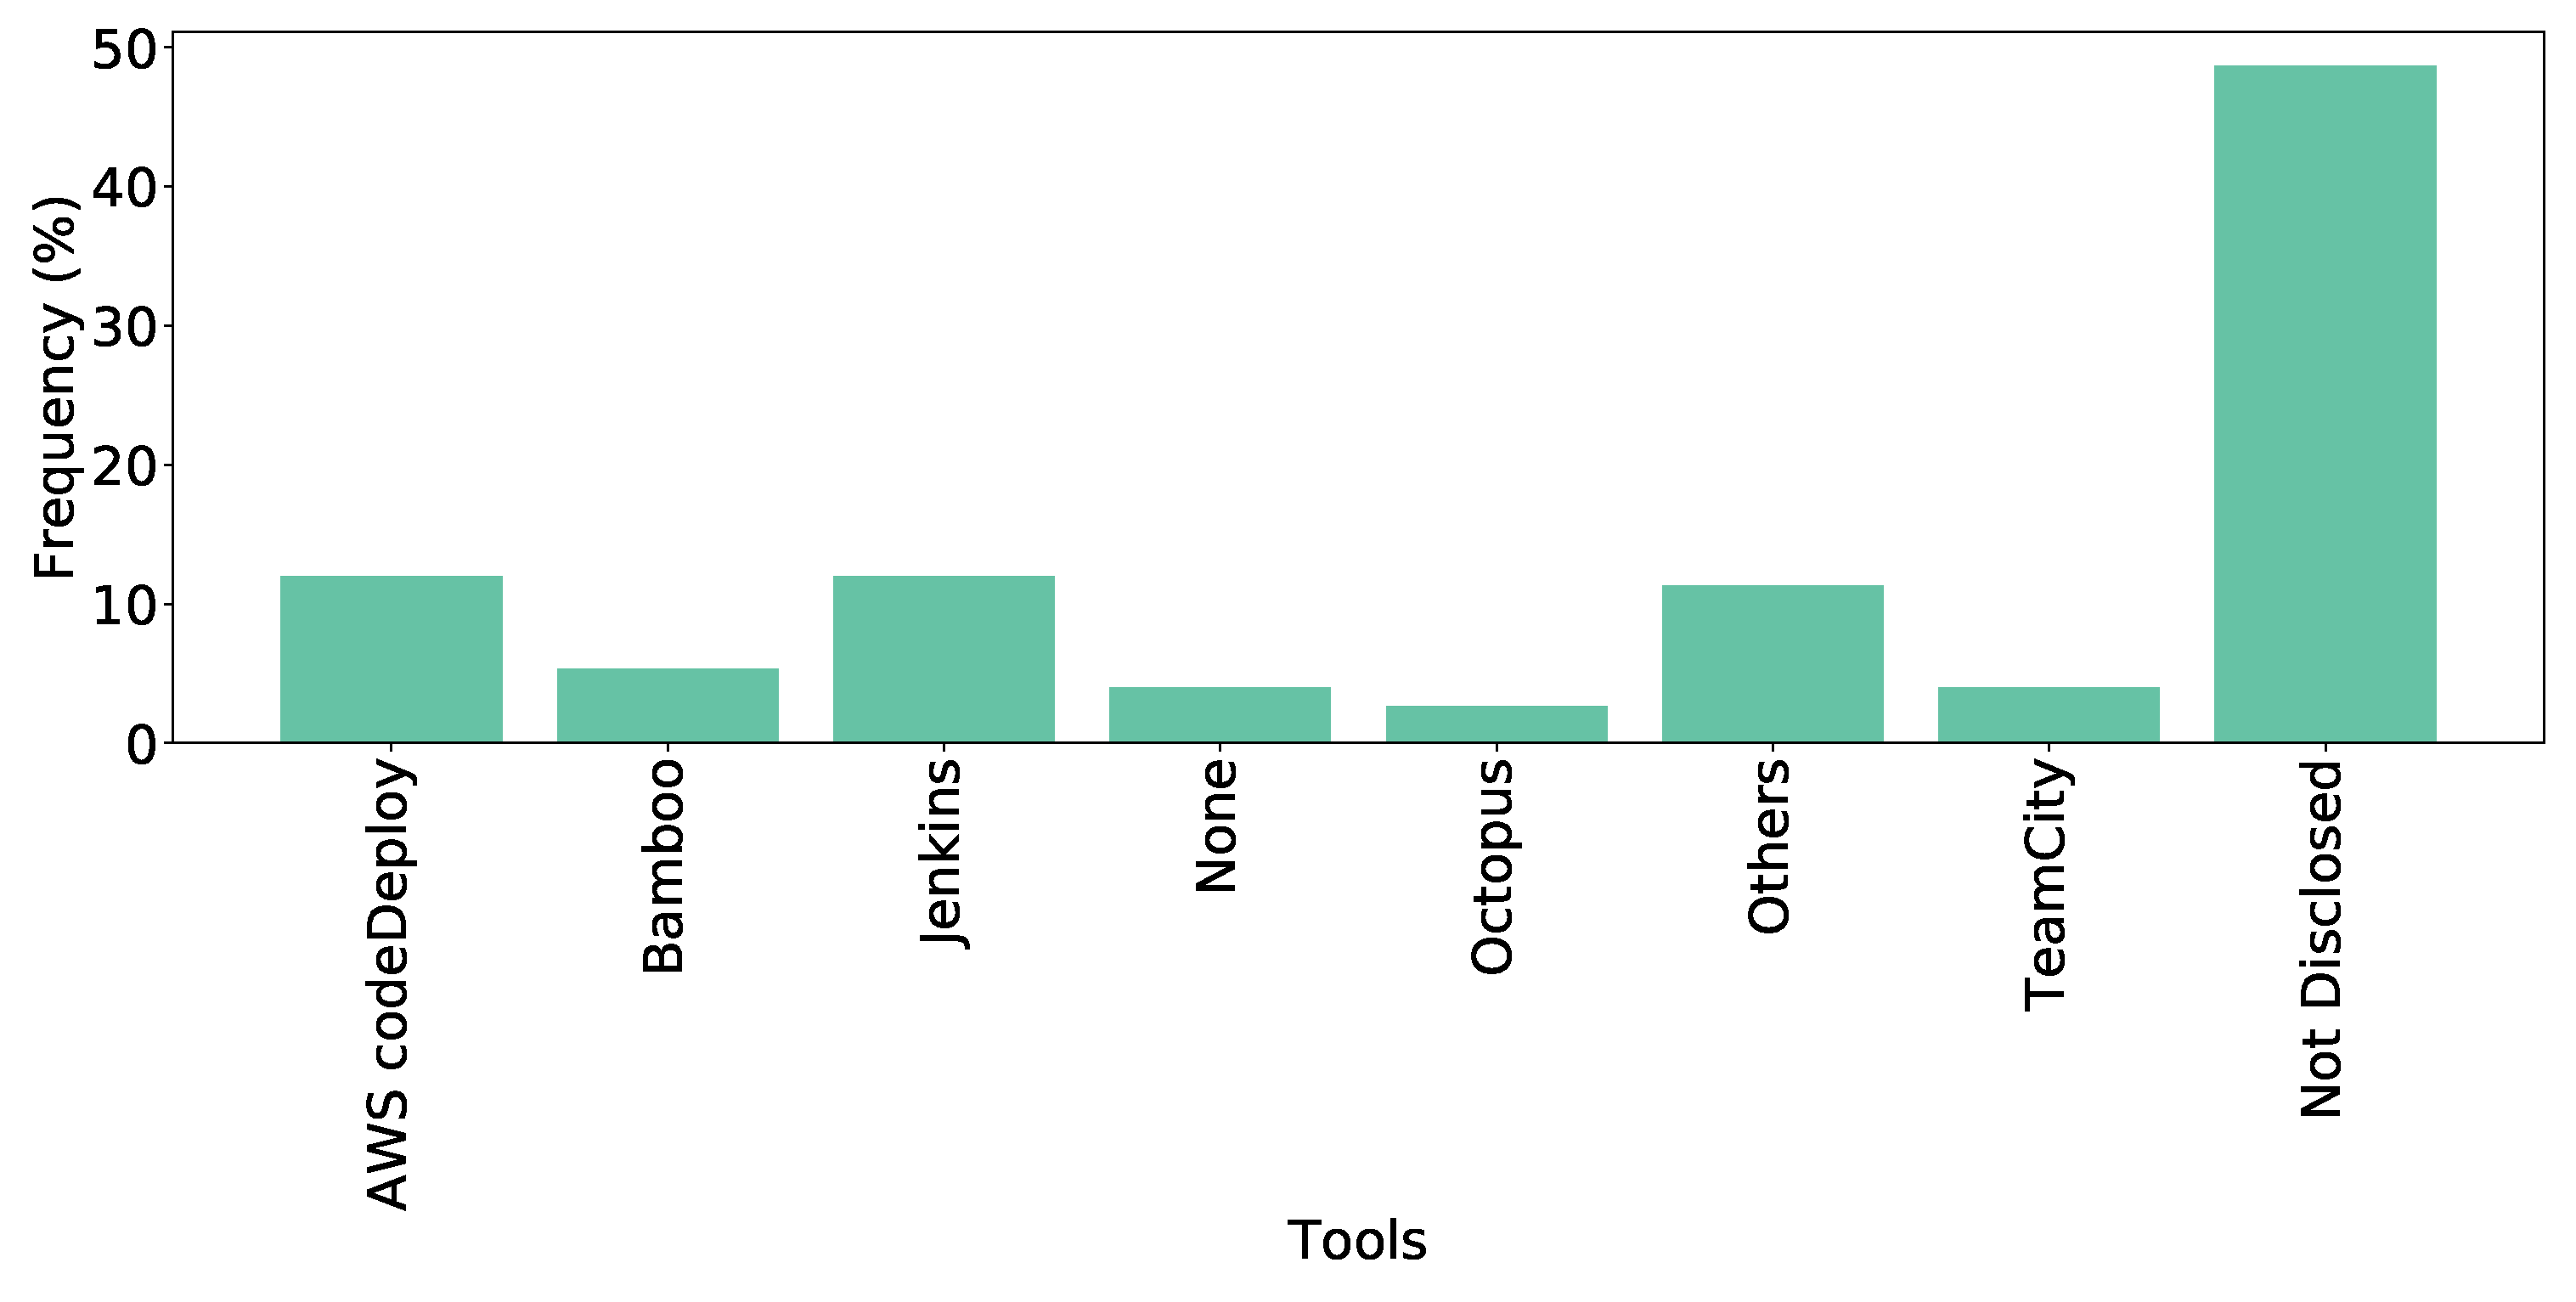
\includegraphics[width=0.8\textwidth]{Figures/Respondents_deployment_tools}
%   \caption{Deployment Tools}
%   \label{fig:deployTools}
% \end{figure}

\paragraph{Version Control}
% \hfill\\
Respondents were allowed to select more than one option. As shown in figure \ref{fig:versionControl}, Git (78\%) and Bit-Bucket (29\%) are mostly-used version control in the software industry. Beside these Subversion (SVN) (5\%), others (4\%) are used.  The 2018 Stack overflow survey\cite{StackoverflowSurvey2018} reports that  the most popular version control system is Git (87.2\% developer uses Git) and the second most popular is SVN (16.1\% developer uses SVN). However, in our survey, we found slightly different result,the most popular version control system is Git and the second most popular is Bit-bucket. This might be related  to the declining popularity of SVN over the years. From the Stack overflow survey over the range 2017-2019, it is clear that SVN is losing popularity to Git. Nowadays, SVN is mainly used for versioning legacy projects. As the SE industry of Bangladesh is quite new, we observe such discrepancy in the popularity of SVN.

% \begin{figure}[htbp]
% \centering
%   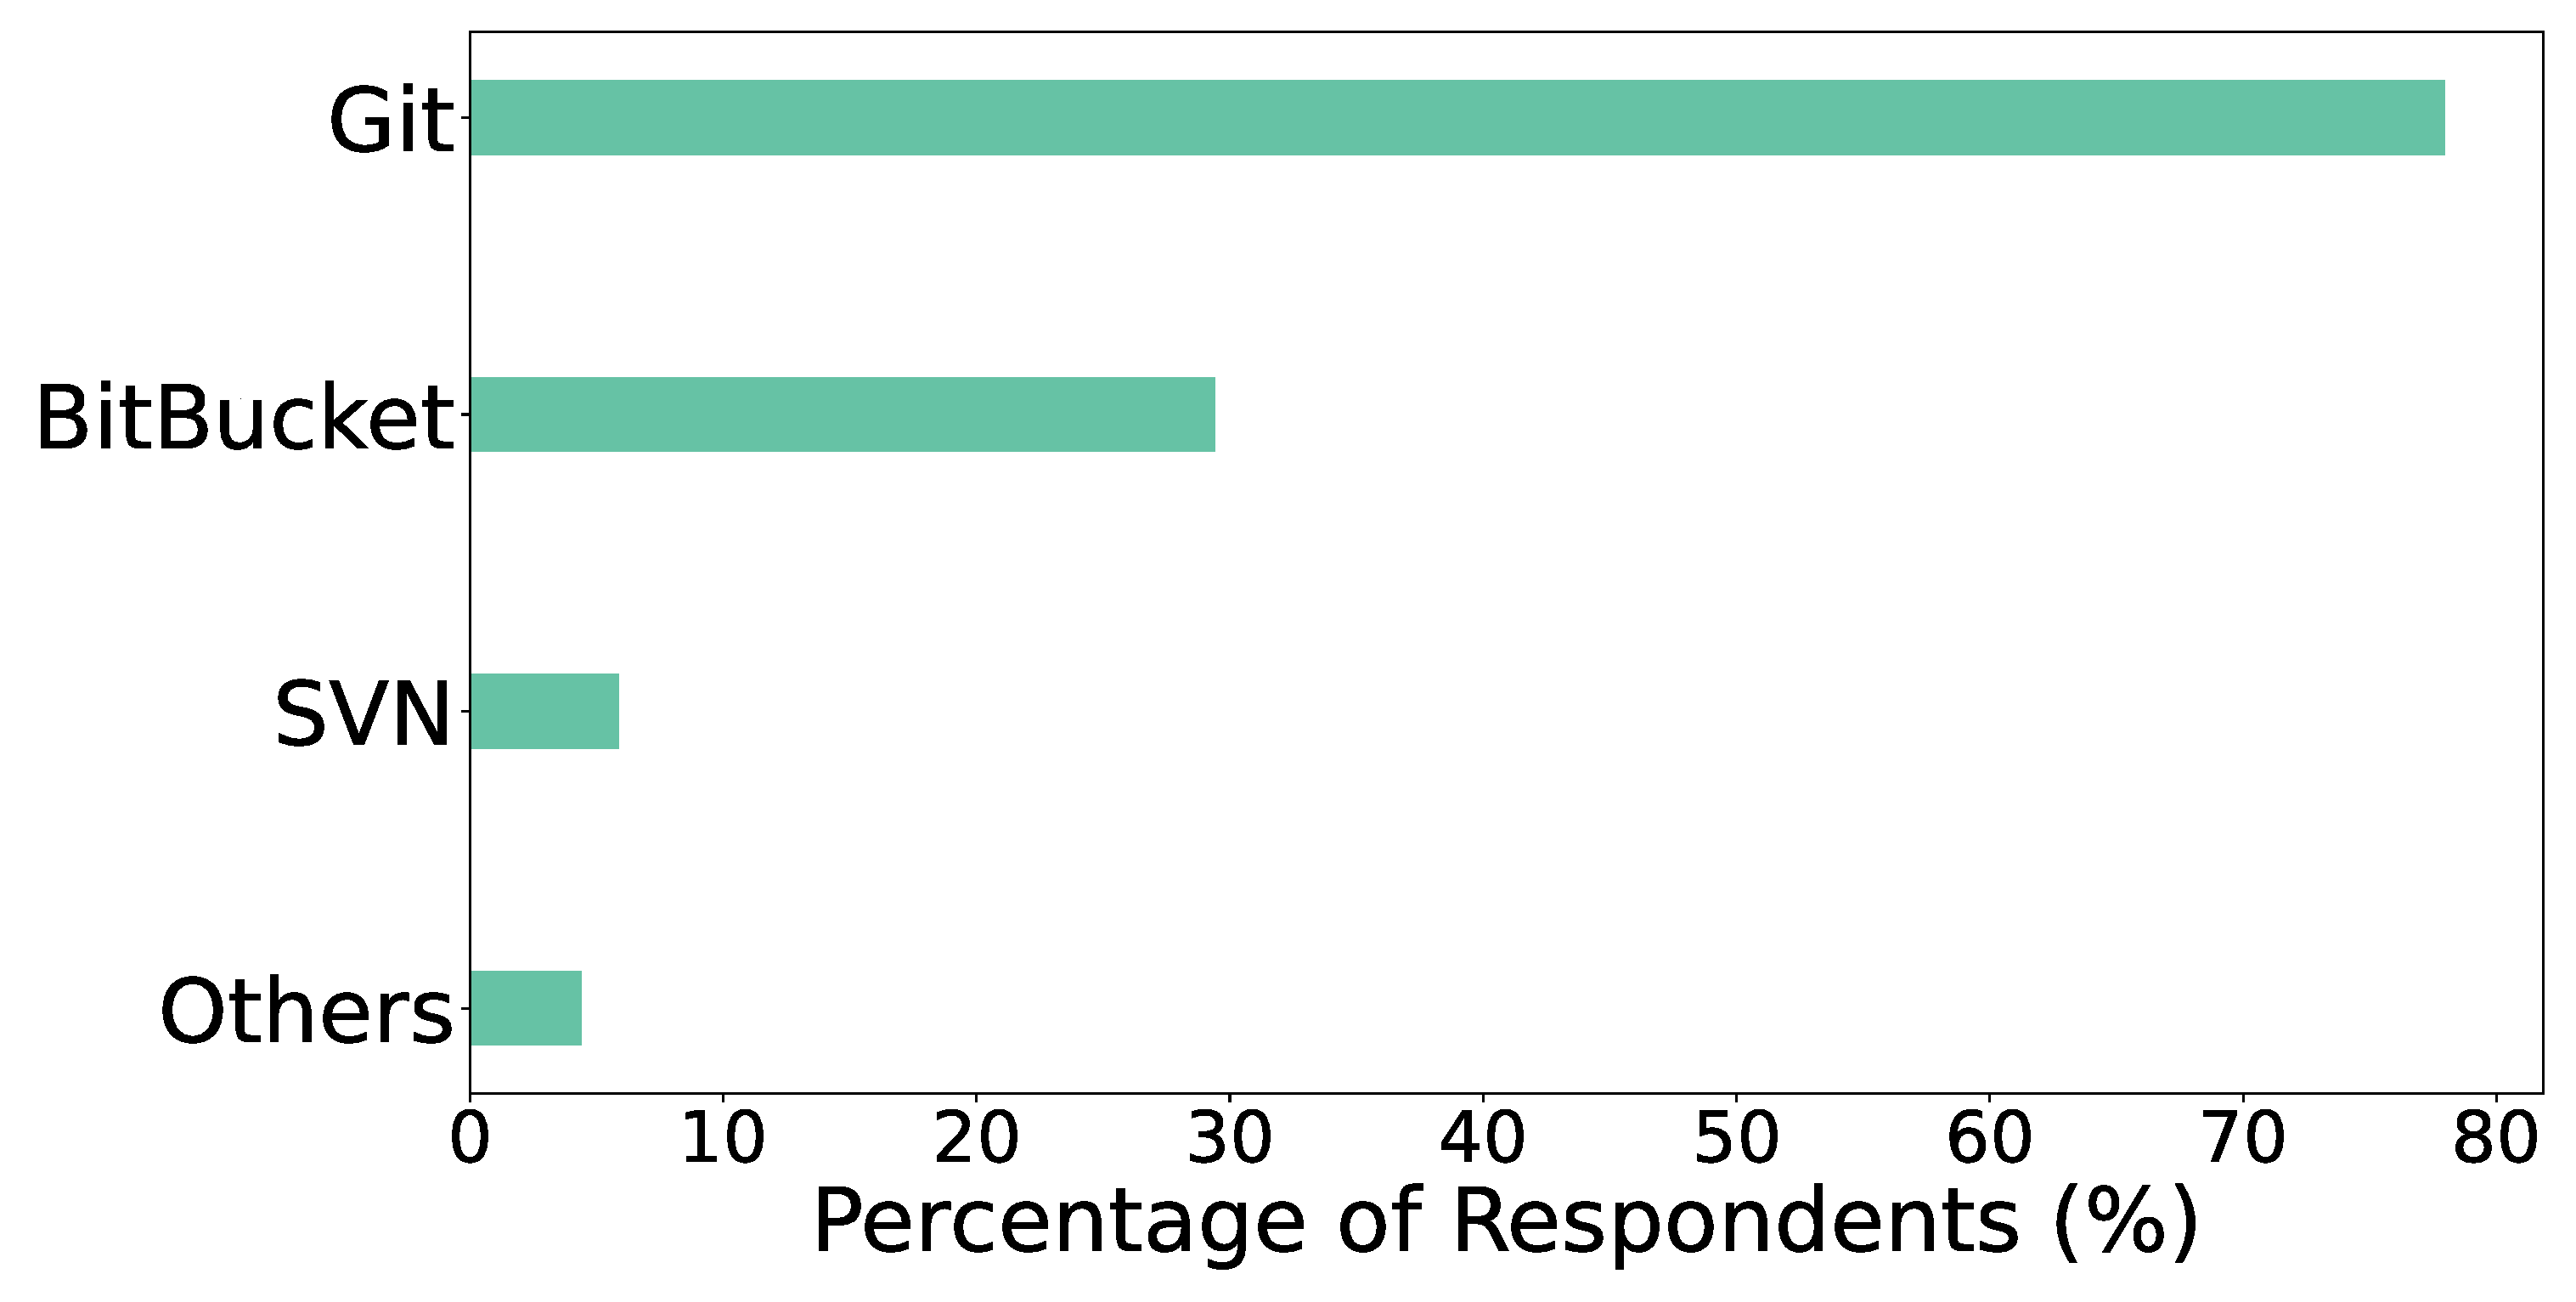
\includegraphics[width=0.8\textwidth]{Figures/Respondents_version_control}
%   \caption{Version Control}
%   \label{fig:versionControl}
% \end{figure}
\subsubsection{How are the security and performance is ensured in a product of a company?}
\label{security_performance}

To identify general practices among the Bangladesh software industry regarding software products' security and performance, we have included two open-ended questions in the survey. This particular question covers how a company secures its code from external attack and maintain its performance after deployment. However, the performance of a software product is related to the scalability of the solution. So, we will cover the following points here:
\begin{itemize}
    \item Security
    \item Performance
    \item Scalability
\end{itemize}


\paragraph{Security:}
\label{Security}
% \begin{figure}[htbp]
% 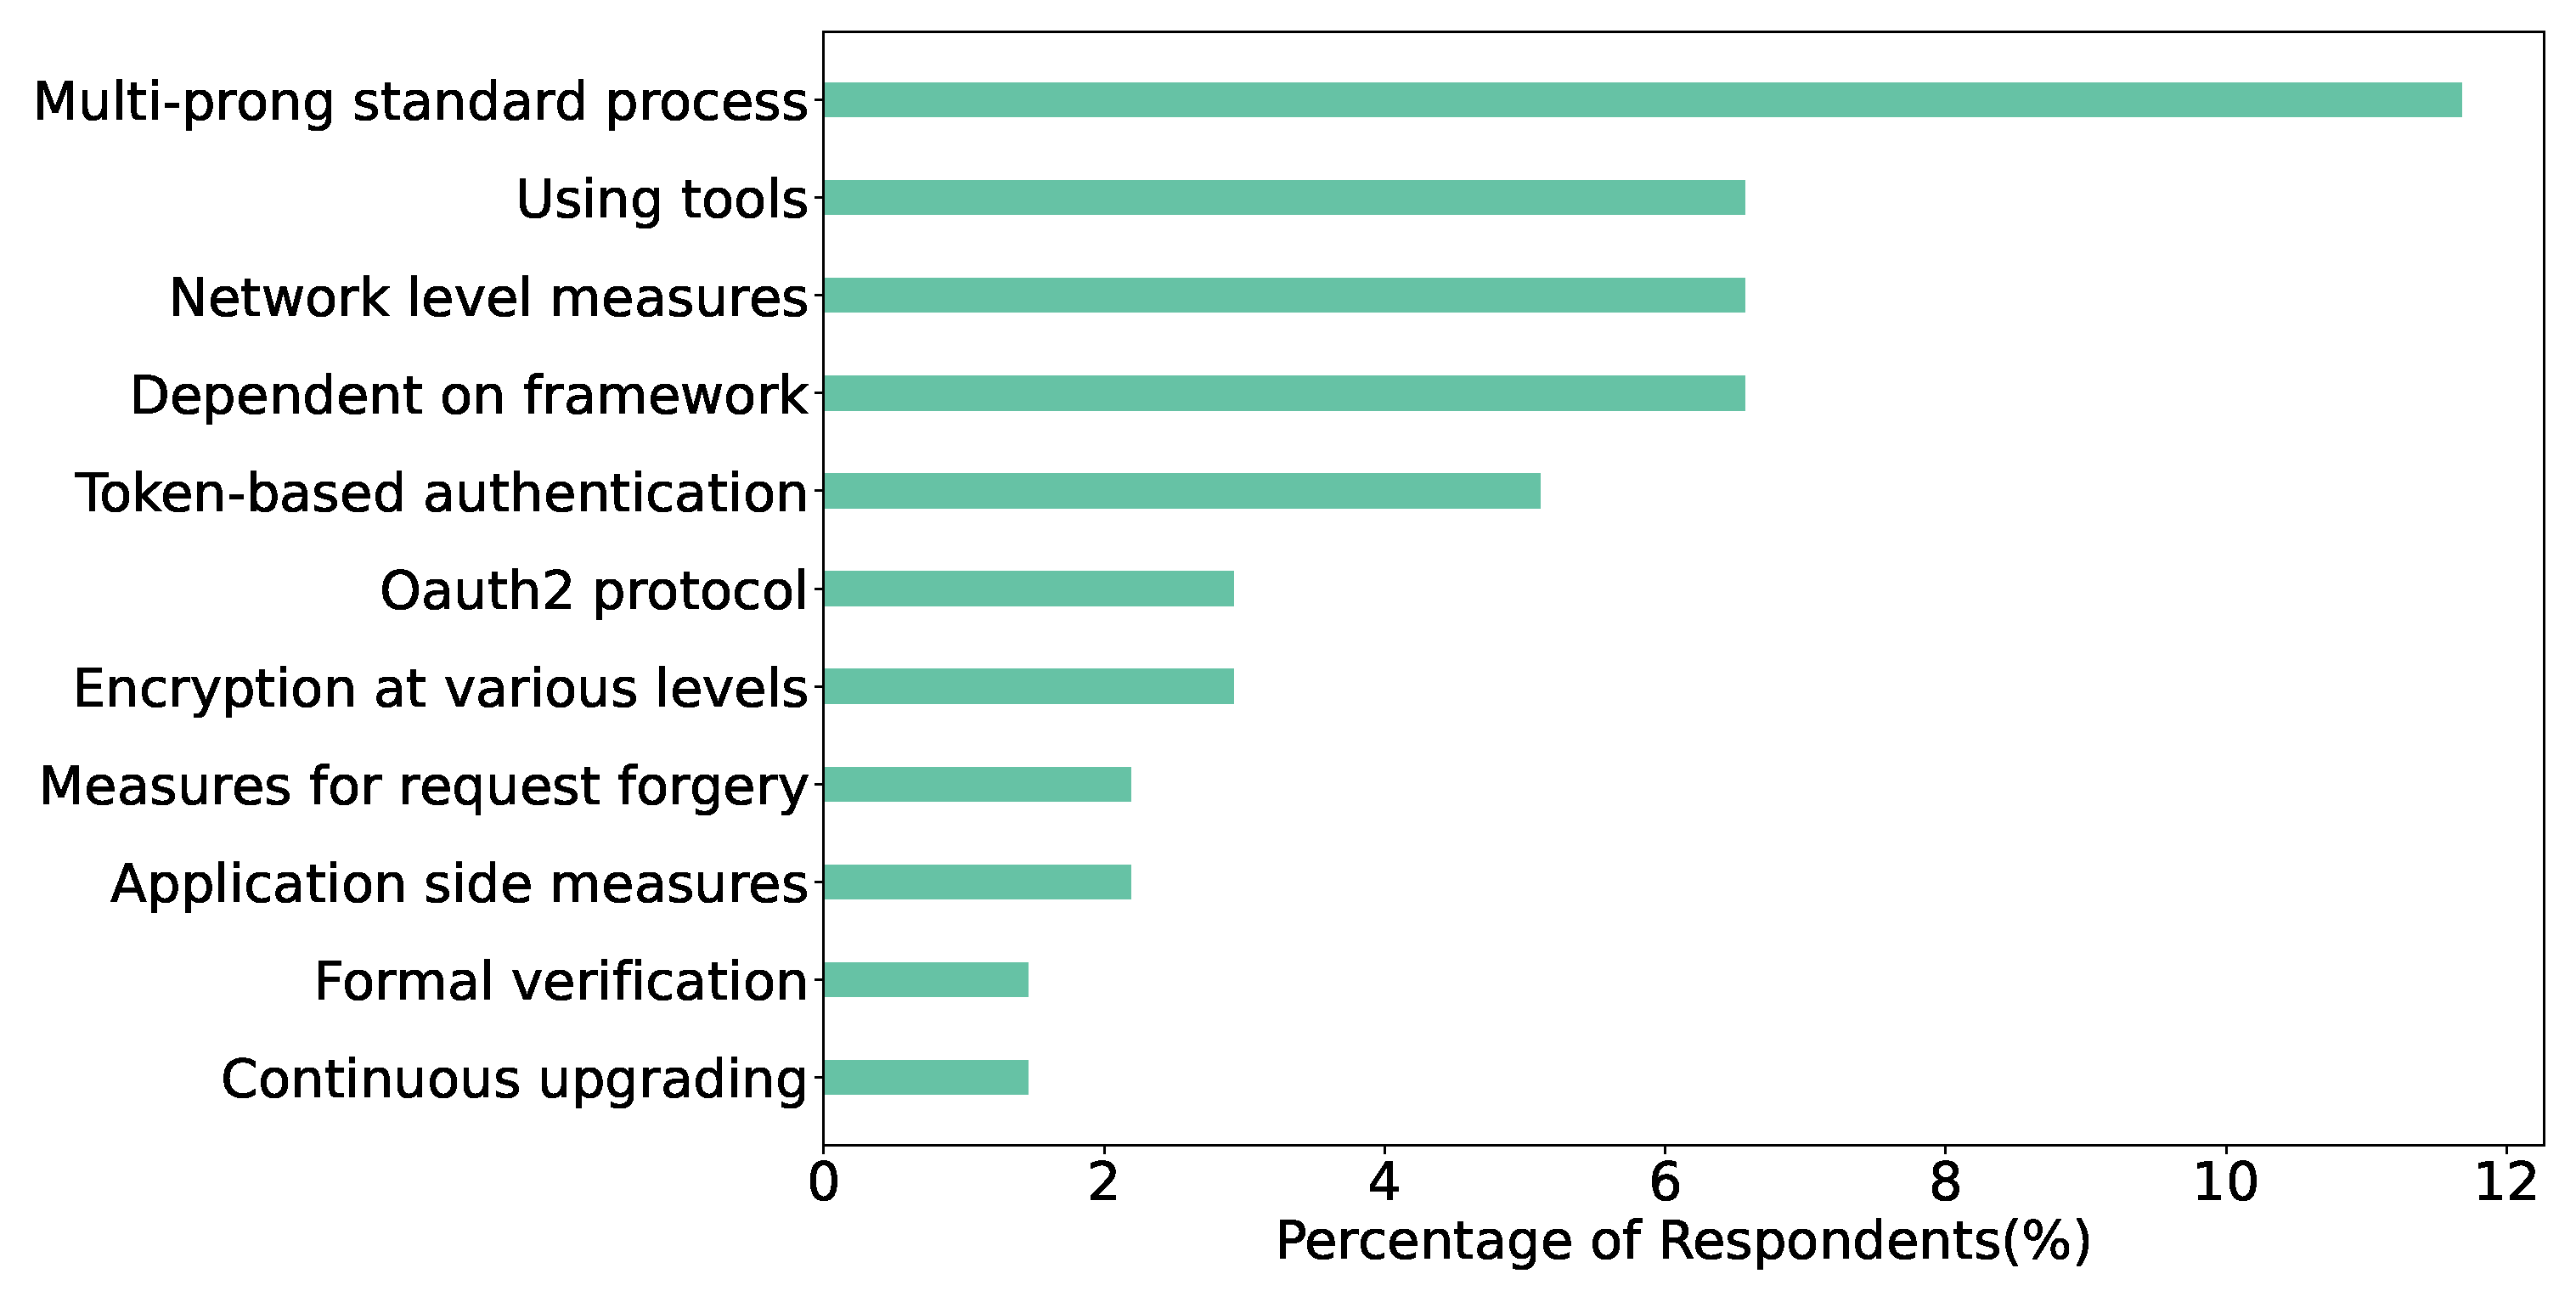
\includegraphics[scale=0.28]{Figures/Security.eps} 
% \caption{Measures to maintain security of products}
% \label{fig:Measures to ensure security}
% \end{figure}
% \hfill\\

Authentication and authorization-based security are the most prominent practice in the Bangladesh software industry to ensure software products' security. The other categories are security based on framework/platform/tools and encryption. Under these categories, several measures are usually followed. The measures of the security categories are discussed below,
Measures under the \emph{authentication and authorization} category is practised by 25.5\% respondents to ensure security. The measures are 
\begin{enumerate}[label=(\alph*)]

    \item \textbf{Multi-prong Standard Process} : About 10.22\% of the total respondents reported that they practices various security standard and protocol to ensure security. The standard includes ISO/IEC 27001 , and PA DSS
    \surveyquote{Multi Prong Standard Processes and Products}{110}
    
    \item \textbf{Token-based authentication} : A token-based authentication system allows users to enter their username and password to obtain a token, which allows them to fetch a specific resource - without using their username and password. Once their token has been obtained, the user can offer the token, which offers access to a specific resource for a time period - to the remote site. 5.11\% of people expressed its eligibility.
    \surveyquote{Token based authentication for all of my rest service}{80}
    
    \item \textbf{OAuth 2.0} : OAuth 2.0 is the industry-standard protocol for authorization. OAuth 2.0 focuses on client developer simplicity while providing specific authorization flows for web applications, desktop applications, mobile phones, and living room devices. Many (2.92\%) respondents use the OAuth 2.0 protocol as the main way of maintaining security.
    \surveyquote{OAuth 2.0, JWT, Token Base Authentication, CORS Filter, XSRF}{127}
    
    \item \textbf{Application Side Measures}: 2.19\% of respondents responded that they implement security measures at the application level. This measure includes encryption of application data at the client-side, use of https while pulling data from a server, secured architecture etc.
    \surveyquote{At application level, could not achieve others yet}{72}
    
    \item \textbf{Measures for request forgery}: Measures against cross-site forgery are implemented to ensure security. This includes CORS or cross-origin resource sharing, CSRF, or cross-site request forgery or one-click attack or XSRF. 2.19\% of respondents implemented measures against  Cross-site request forgery to ensure security.
    \surveyquote{Security testings like: SQL injection, cross-site scripting, CSRF, API security, use of https,  detecting malicious / suspicious HTTP requests and auto-blocking}{42}
    
    \item \textbf{Formal Verification}: A code-level review can mitigate security threats. 1.46\% respondents ensured the practice of formal code review.
    \surveyquote{There are some basic guidelines that we must follow and while code review this needs to be an absolute part that needs to be checked before the code gets merged}{112}
    
\end{enumerate}

21.17\% respondents use several technology, tools,platform to ensure security of their product. Measures under the \emph{framework/platform/tools} category are,
\begin{enumerate}[label=(\alph*)]

     \item \textbf{Dependent on Framework} : The common frameworks provide basic to intermediate level security measures in the application. 6.57\% of respondents depend on the framework for security. The framework includes popular frameworks such as spring and  HDIV.
    \surveyquote{https, popular framework which already prevents some type of attacks. rest of the things on case-by-case basis)}{79}
    
    \item \textbf{Use of tools} : Respondents use various open-source/ paid tools for scanning and testing. These tools help to find security threats in an existing system. The tools include OWASP based tools and  penetration testing tools.
    \surveyquote{use encryption at different level of software (server, network, transmission layer, database and software layer.)}{35}
    
    \item \textbf{Network level Measures}: Network-level measures include IP-white-listing, port-blocking, VPN, and use of HTTPS  in software. 6.57\% of respondents use at least one of the before-mentioned strategies to ensure security.
    \surveyquote{network blocking and common security measures}{2}

    \item \textbf{Continuous Upgrading}: As security threats are evolving; thus, current systems need continuous up-gradation in a frequent interval. 1.46\% of respondents said they arrange frequent hackathons, workshops, and security audits to address the continuously evolving security threat.
    \surveyquote{We run security audit of our office environment. We also conduct security session per 6 months to introduce latest trend in threats and what we can do to avoid it}{57}

\end{enumerate}

2.92\% of respondents use encryption technologies to encrypt their data. Respondents use encryption at the different levels of software architecture such as network, data, transmission, and ensure their security.
\surveyquote{use encryption at different level of software (server, network, transmission layer, database and software layer.)}{35}

% To maintain security of software product SE industry of Bangladesh is mainly dependent on standard process which includes cloud based security, third party software, OS hardening followed by uses of security tools, network level measures and framework security. As found by Harrison et al.\cite{Harrison2010} network level measures are the first choice in ensuring security of software product which matches with our findings. Srinivasan et al.\cite{Srinivasan2017} listed top 10 web framework in terms of security testing where Spring framework achieved 7\textsuperscript{th} position. From figure ~\ref{fig:frameworks} we have seen that most of our respondents use Spring framework for software development. This might be the reason that a lot number of respondents dependent on framework for ensuring security.


\paragraph{Performance}
\label{Performance}

% \begin{figure}[htbp]
% 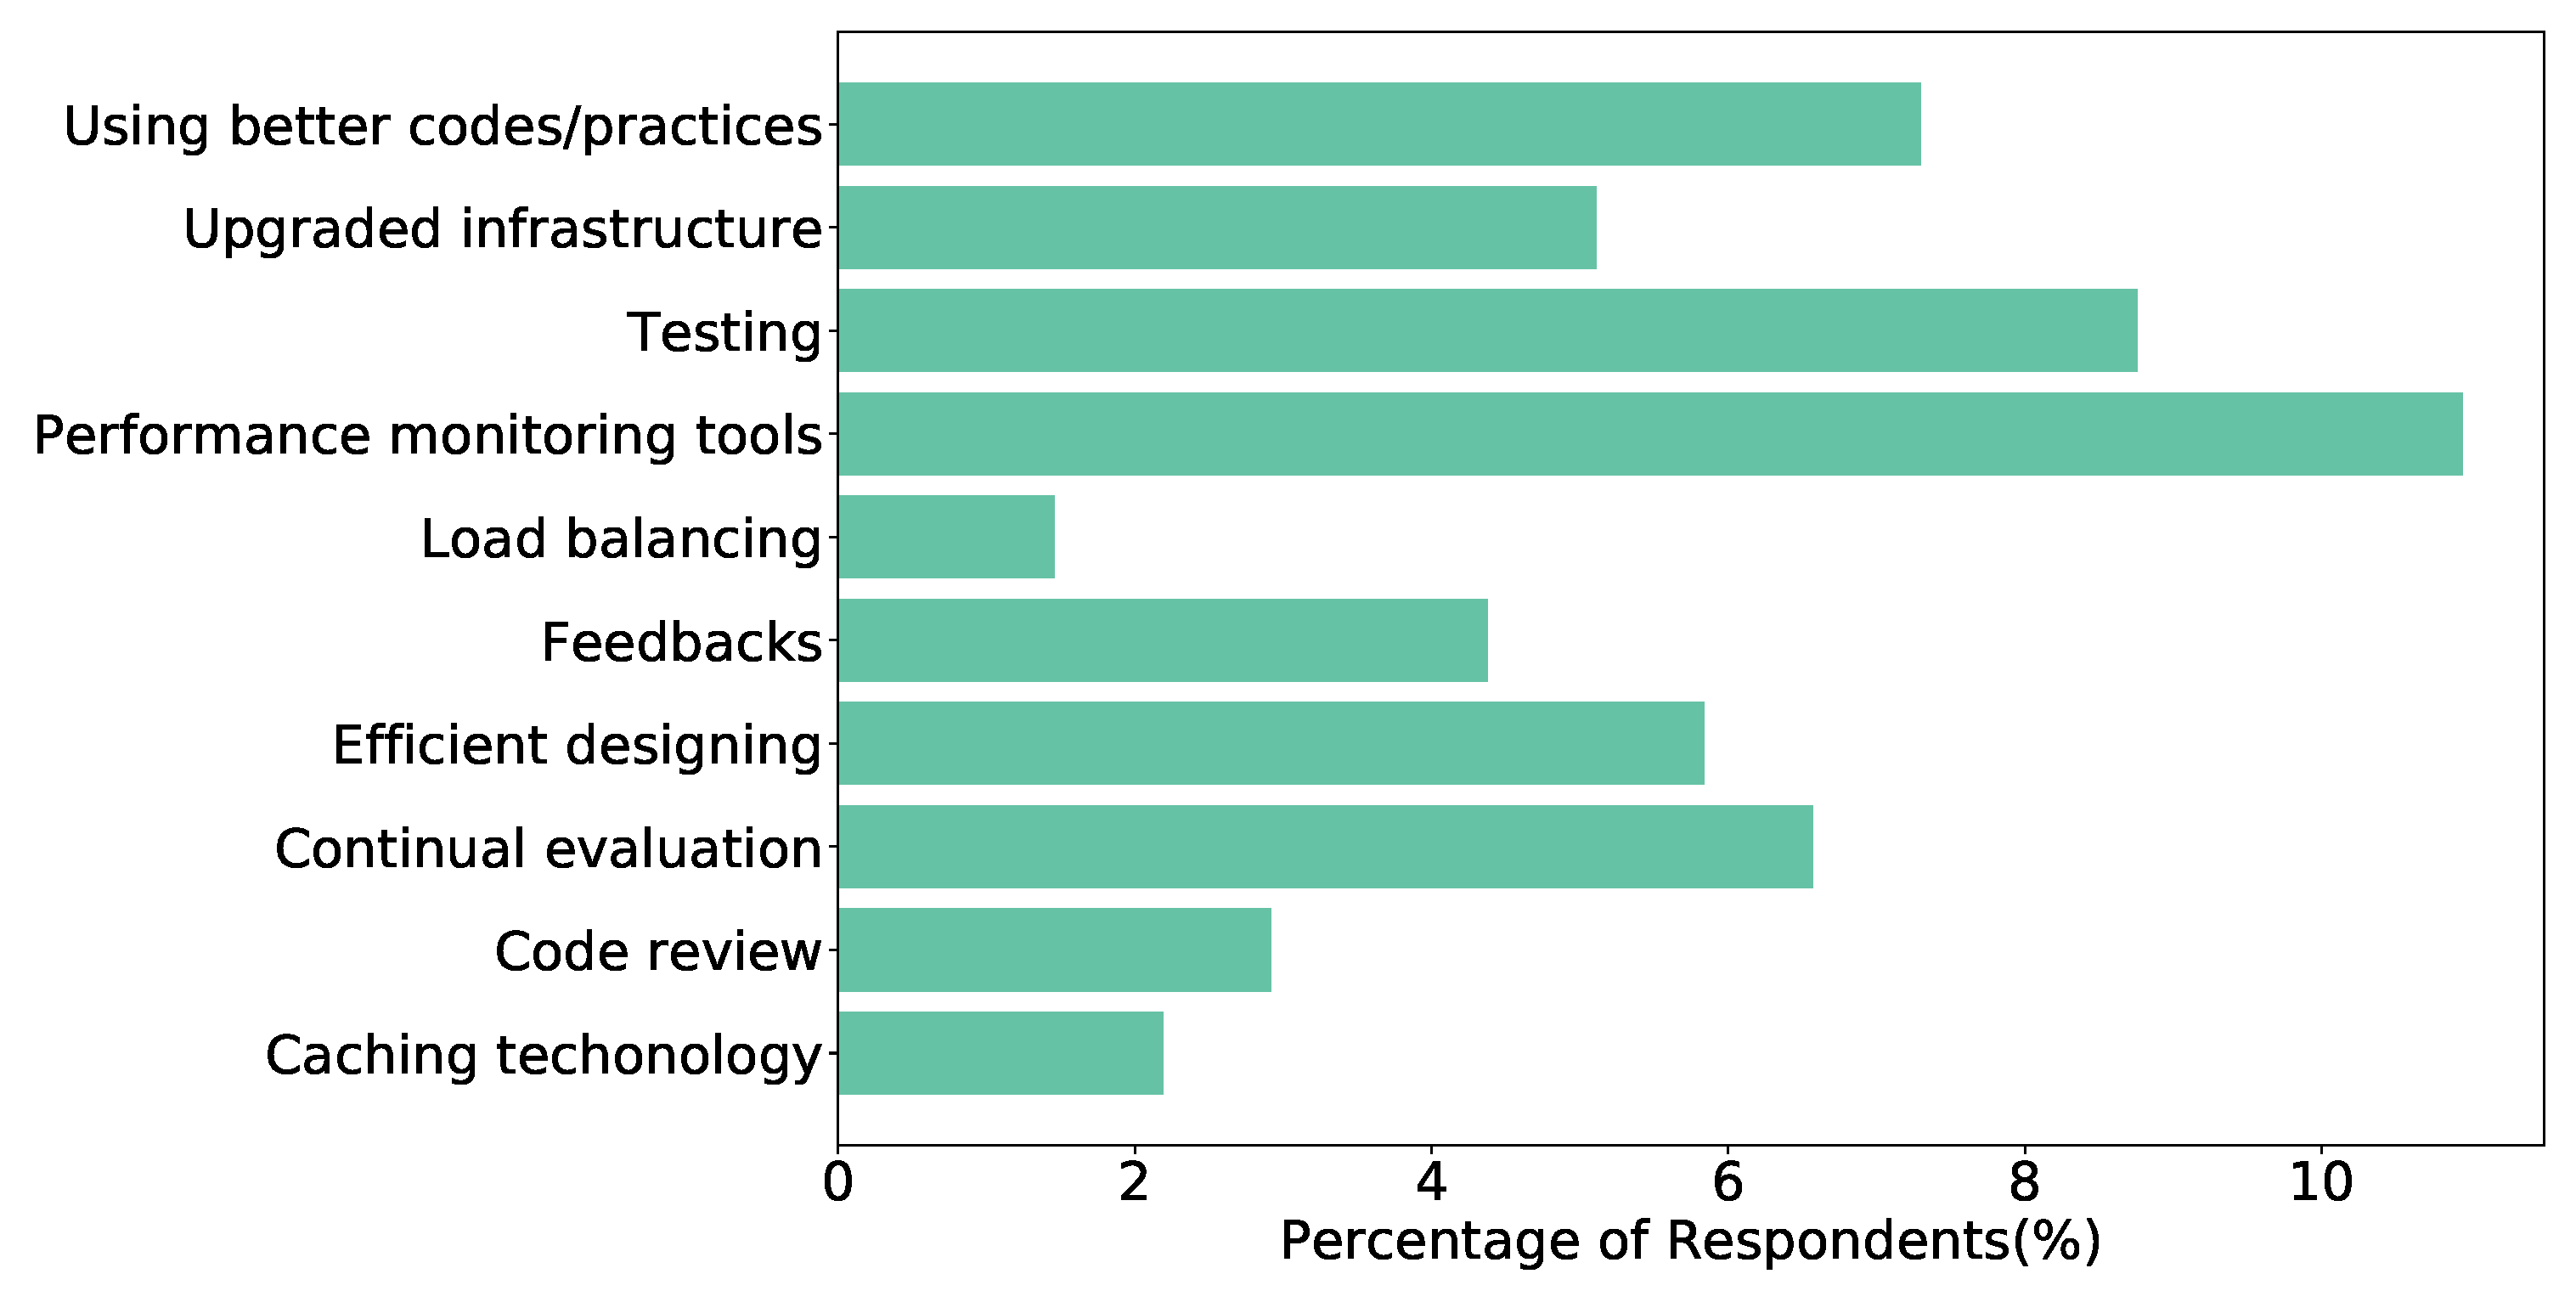
\includegraphics[scale=0.28]{Figures/Performance.eps} 
% \caption{Measures to ensure performance of products}
% \label{fig:Measures to ensure performance}
% \end{figure}
% \hfill\\

Software performance indicates how efficient the software is in terms of resources and time. Use of framework/tools/platform to ensure software performance is a dominant practice in the Bangladesh SE industry. The other type of practices is peer-review, software design, and software testing. Respondents in our survey reported multiple measures under these categories. The measures in \emph{framework/tools/platform} category are,
\begin{enumerate}[label=(\alph*)]

    \item \textbf{Load Balancing}: Load balancing can improve the system performance by ensuring an equal load to all servers. 27.1\% of respondents think of using load balancing as a measure to maintain performance.
    \surveyquote{Optimizing number of HTTP requests, Asynchronous programming, Caching, CDN, Load Balancing, nginx, varnish, compression of data, Continuous monitoring, Load testing, stress testing}{42}
    
    
    \item \textbf{Performance Monitoring Tools}: There are various performance monitoring automated tools from which we can measure the overall and component-wise performance. 10.95\% of respondents use these tools to measure performance. Respondents use several performance metrics such as error/crash rate, response time, uptime, etc.
    \surveyquote{take help of different performance monitoring tools and dashboard, analyzed data , measure time and memory efficiency of process}{35}
    
    \item \textbf{Upgraded Infrastructure}: 5.11\% of respondents use upgraded infrastructure to ensure performance. This infrastructure includes cloud hosting, a high-end server, and new technologies.
    \surveyquote{Amazon Hosting and Quality Software}{85}
    
    \item \textbf{Caching Technology}: Caching mechanism improves performance by reducing response time. 2.92\% of respondents rely on caching to maintain software performance.
    \surveyquote{... Good Caching}{29}

\end{enumerate}


13.14\% of respondents ensure software performance  at design phase. Measures of this category are,

\begin{enumerate}[label=(\alph*)]

    \item \textbf{Using better codes/practices}: Industry-standard best practices can improve system performance. 7.3\%respondents ensure performance by implementing best practices. The best practices include compression technology, enforcing design patterns, and refactoring.
    \surveyquote{Implementation time carefulness and maintaining a well developed coding standard}{40}
    
    \item \textbf{Efficient designing}: Software performance is dependent on the architecture of the system. 5.84\% of respondents emphasize design to ensure performance.
    \surveyquote{By careful designing}{24}

\end{enumerate}

 8.76\% of respondents of our survey rely on the software testing strategy to ensure performance. Performance is ensured by various rigorous testing phase. The phase includes load testing, stress testing, integration testing.
 \surveyquote{By rigorous testing and checking performance testing}{17}
 
 Reviewing peer and user, tester feedback can be a good strategy to ensure performance. 7.3\% of our respondents use measures from this category to ensure performance. Measures under this category are,
 
 \begin{enumerate}[label=(\alph*)]
 
     \item \textbf{User Feedback}: It is a great source of performance measure. Taking time to time feedback from the clients helps a company realize how their products are performing. Many (4.38\%) respondents have highly recommended it.
    \surveyquote{Continuous feedback from clients and QA team}{65}
    
    \item \textbf{Code Review}: About 2.92\% of people have said that a proper and attentive code review can reduce the codes' faults and, therefore, enhance the performance of a software.
    \surveyquote{The code quality is assessed by the different team members during code review, followed by designing new ways to solve issues in the product that are time-intensive.}{15}
 
 \end{enumerate}



\paragraph{Scalability}
% \label{Scalability}
% \begin{figure}[htbp]
% 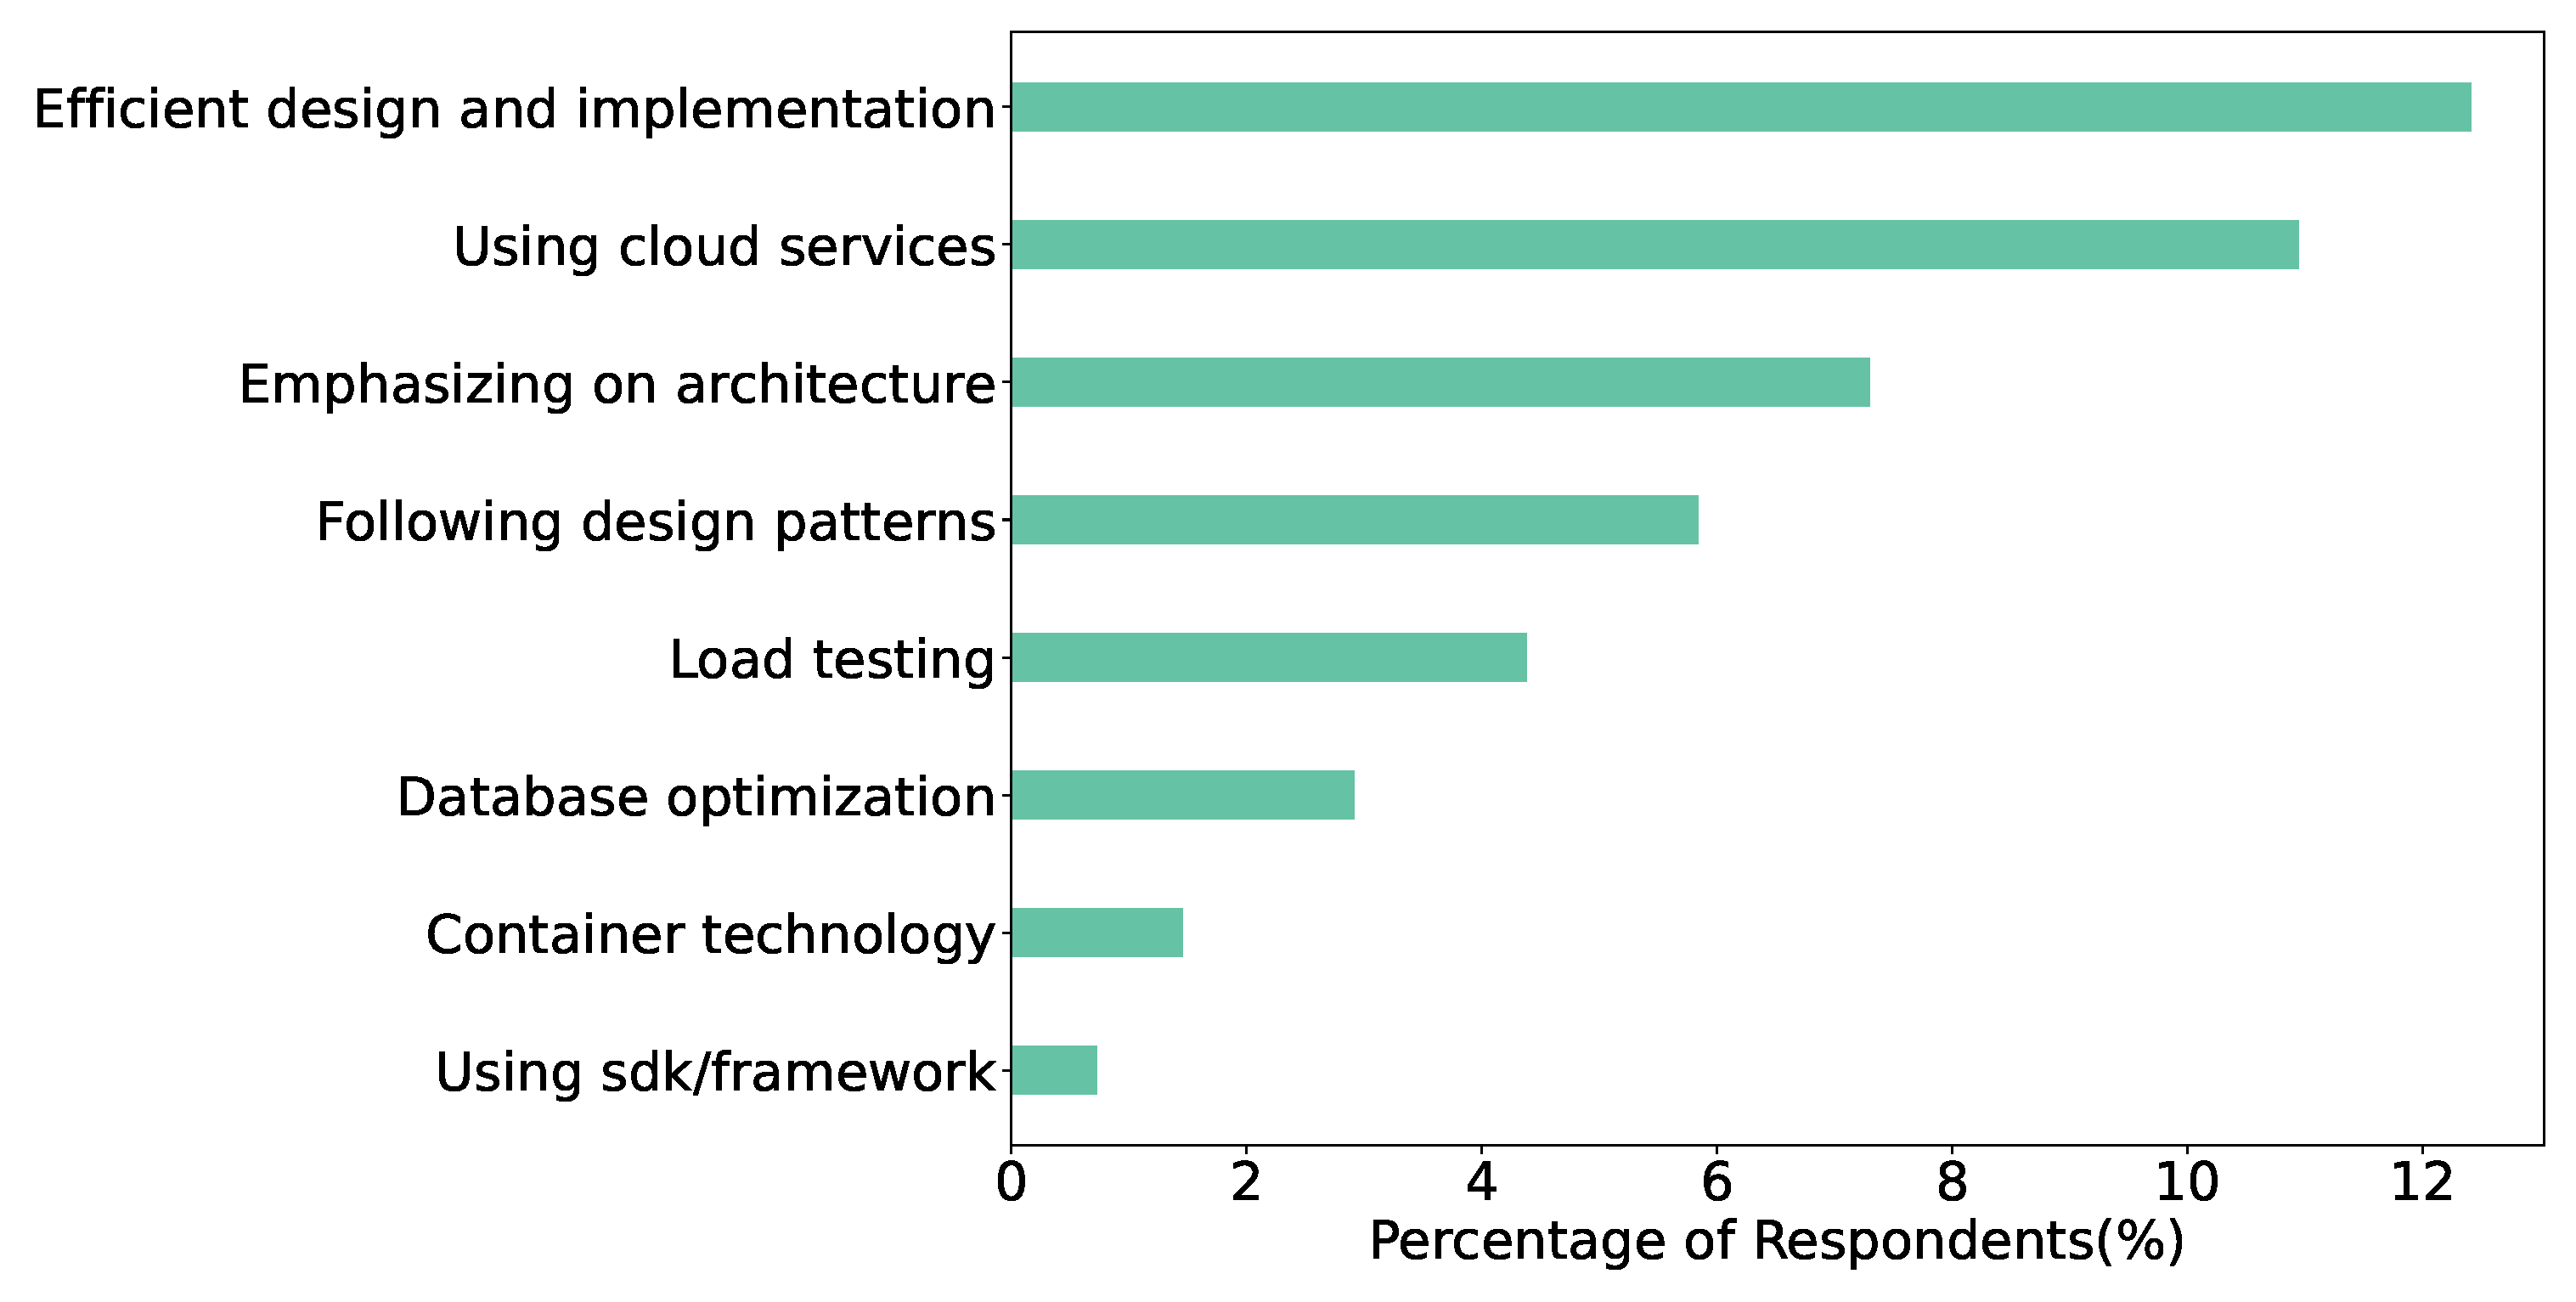
\includegraphics[scale=0.28]{Figures/Scalability.eps} 
% \caption{Measures to ensure scalability of products}
% \label{fig:Measures to ensure scalability}
% \end{figure}
% \hfill\\

 Software scalability defines the ability to scale up a solution. Issues with little importance can impede scaling up. Thus proper measures should be taken from the design stage to ensure the scalability of the system. Scalability ensured by efficient software design is the most practices strategy in the Bangladesh SE industry. 25.55\% reported using at least one of the measures in this category. The measures are,
% Recent days the cloud services offer tools to accomodate custom reactive scaling strategies. Thus, it has become easier to ensure scalability using cloud services \cite{Falatah2014}. Our results  also follows the world trend, usage of cloud services has placed 2\textsuperscript{nd} in terms popularity of scalability measures in SE industry of Bangladesh.
 \begin{enumerate}[label=(\alph*)]
 
     \item \textbf{Efficient Design and Implementation}: 12.41\% of respondents emphasize on the design and implementation of a scalable architecture. 
    \surveyquote{During implementation we always keep in mind about the scaling factor}{40}
    
     \item \textbf{Emphasizing on architecture}: 7.3\% of respondents emphasized on architecture. It is mostly micro-service architecture which they use to ensure scalability.
    \surveyquote{We follow the micro-service architecture. In a nutshell, we scale up the module vertically which is necessary. We use docker along with Jenkins for automatic deployments and scaling.}{10}

    
    \item \textbf{Following Design Patterns}: Some design patterns inherently help in the time of scaling. 5.84\% of respondents think that following these design patterns will be of great use for software scalability.
    \surveyquote{Following certain design patterns}{8}
 
 \end{enumerate}
 
 13.14\% of respondents of our survey use framework or some kind of tool to ensure scalability. The measures in this category are,
\begin{enumerate}[label=(\alph*)]

    \item \textbf{Using Cloud Services}: 10.95\% user depends on cloud services like AWS and Azure for the scalability of the system. Modern features like elastic load balancing and auto-scaling make it easy to ensure scalability.
    \surveyquote{Using AWS Elastic Load Balancer}{28}
    
    \item \textbf{Container Technology}: Container technologies include Docker, Kubernetes, which ensure OS-level virtualization. By standardizing the system, container technologies ease the scaling of an infrastructure.1.46\% of respondents use these measures to ensure product scalability. Containers enable users to scale their system without any worries about the underlying OS.
    \surveyquote{We used Docker technology}{85}
    
    \item \textbf{Using SDK/framework}: Modern frameworks ensure scalability by default. 0.73\% of respondents solely depend on the framework for scalability.
    \surveyquote{following flexible framework which allows better scalability}{14}
  
\end{enumerate}
 
 
There is one measure under the software testing category, which is load testing. Load testing can be used to check the scalability of a system. 4.38\% of respondents use load tests to check whether their system is scalable or not.
\surveyquote{through load testing and load simulation.}{35}

There is also one measure under the Database Design category, which is database optimization. Database optimization includes sharding, clustering, indexing, and scaling. 10.3\% of respondents optimize database to scale their system.
\surveyquote{Besides scaling horizontally, database scaling is performed by partitioning tables, along with multi-threaded implementations}{85}


% \subsection{Comparison among countries (RQ2)}
\label{RQ2}

In this section, we present a comparative discussion on different dimensions of software development practices and processes among different regions of the world along with Bangladesh. We do the comparison along the following dimensions:

\begin{itemize}
    \item Development methods and practices
    \item Implementation technologies
    \item Quality assurance
    \item Release and iterations
\end{itemize}

The following subsections describe these dimensions.

\subsubsection{Development methods and practices}
\label{dev_methods}

To find out the overall comparison of this section, we report the following sub-sections:

\begin{itemize}
\item Software development methodologies (Q 6).
\item Requirements gathering (Q 7).
\item Most time consuming software development activities (Q 8).
\end{itemize}

\paragraph{Software development methodologies}
From the study we see that the most acceptable model that was regularly and always used is the agile model (64\%) in Bangladesh but the usage of the scrum (44\%) in New Zealand has greater usage followed by agile (30\%) \cite{Wang2018} and in Turkey, waterfall is mostly used based on the earlier 2015 survey \cite{Garousi2015}. Again, in both Bangladesh and New Zealand, extreme programming (XP) has a lower percentage of usage.

\paragraph{Requirements Gathering}
According to \ref{fig:requirements}, using plain text (44\%) and story board (41\%) are the most widely used requirements gathering. This result is similar with the survey of Vonken et al. \cite{Vonken2012}. From their study we can find that the textual description of specifying requirements is a firm favourite in Netherlands.

\paragraph{Development activities timeline}
According to study \cite{Wang2018}, most time was spent on implementation and coding and also relatively less time was spent on maintenance in both Bangladesh and New Zealand. But requirement analysis, the activity, requires the second most time to spend in Bangladesh according to 45\% respondents where in New Zealand, it is testing (36\%) practices.

\subsubsection{Implementation technologies and tools}
\label{implementaion_techonologies}

To find out the overall comparison of this section, we report the following sub-sections:
\begin{itemize}
\item Technology Platform (Q 9).
\item Operating System (Q 10).
\item Programming Language (Q 11).
\end{itemize}


\paragraph{Technology Platforms}
As shown in \ref{fig:platforms}, most of the respondents (80\%) worked in web platform. Most respondents develop products and services for web platforms in both Bangladesh and New Zealand based on \cite{Wang2018}.

\paragraph{Operating Systems}
Windows is mostly used among developers of New Zealand based on the survey \cite{Wang2018}, but Linux is mostly used in the case for Bangladeshi developers.

\paragraph{Programming Languages}
Based on \cite{Wang2018}, Java ranks quite low in New Zealand where it is the second most used in Bangladesh and the mostly used language in Turkey \cite{Garousi2015}. Again, python did not get a respective place in the rank of used languages in New Zealand but it is used significantly in Bangladesh.

\subsubsection{What type of testing and deployment practices are used?}

To get the picture of quality assurance (QA) in countries such as Malaysia, Turkey, France, etc., different studies have been carried out. In Table \ref{table:testing_comparison}, we compare the major outcomes of testing and deployment related responses from our study with the similar results of the previous studies. The comparative picture is discussed below.

\begin{itemize}
    % \item Requirements Clarity
    \item Software Testing Practices (Q14)
    \item Level of Automated Testing (Q15)
\end{itemize}

\begin{table}[]
\caption{Comparison of testing practices and test automation between our findings and prior findings}

\begin{tabular}{llll}

\hline
\multicolumn{1}{c}{\textbf{Practices}} & \multicolumn{1}{c}{\textbf{Our Study}} & \multicolumn{1}{c}{\textbf{Prior Study}} & \multicolumn{1}{c}{\textbf{Comparison}} \\ 
\hline 


\multicolumn{1}{l|}{\multirow{2}{*}{\parbox{0.1\textwidth}{What type of testing and deployment practices are used?}}
} 
& 
\multicolumn{1}{l|}{\multirow{2}{*}{\parbox{0.25\textwidth}{
\vspace{-50pt} (1) Around half of our respondents responded about carrying out unit testing and functional testing. Also, the utilization rate of acceptance and UI testing has an appreciable percentage in Bangladesh. (2) Automated testing exercise is not usual in Bangladesh as per the majority of our respondents.
}}
} 
& 
\multicolumn{1}{l|}{\comparisoncell{0.25}{\vspace{50pt}Unit testing is observed to be the most exercised in Malaysia (68.29\%) \citep{Baharom2006}, Canada (79.27\%) \citep{Garousi2013}, New Zealand (73\%) \citep{Wang2018} in a great percentage.
}}                                  

&

\multirow{2}{*}{\parbox{0.23\textwidth}{
\vspace{-70pt} We have perceived that unit testing is moderately practiced in Bangladesh, though its usage is comparatively spacious in other countries. In the adoption of test automation, the software industry of Bangladesh is way behind France though the usage rate might have similar to other European countries.
}} \\ \cline{3-3}

\multicolumn{1}{l|}{}                                       
& 
\multicolumn{1}{l|}{}                                       
& 

\multicolumn{1}{l|}{\comparisoncell{0.25}{
\vspace{50pt} Test automation is highly embraced by France software industry and comparatively less adopted in overall Europe~\citep{dutta1999}.
}} 
&                                         
\\ \hline

\end{tabular}
\label{table:testing_comparison}
\end{table}



\paragraph{Software Testing Practices}
From our study, as per \ref{fig:testing}, we see an interesting point that unit testing (53\%) and functional testing (49\%) are moderately used in Bangladesh, whereas from \citep{Garousi2013} and \citep{Wang2018} we can see that relatively a high percentage of their survey respondents in both Canada New Zealand rely on unit testing with 79.27\% and 73\% respectively. On the other hand, the adoption of acceptance testing and UI testing is quite similar to these countries. In Malaysia, based on \citep{Baharom2006}, Baharom et al. reported that, according to their survey, unit testing (68.29\%), integration testing (78.05\%), system testing (85.37\%), and acceptance testing (78.05\%) are used by most organizations in a high percentage, and about half of the organizations are carrying out alpha and beta testing.

\boxtext{Software developers around the world usually give unit testing the top priority, but the developers in Bangladesh have comparatively less participation.}
\rifat{Is the above observation correct? 53\% usage of unit testing reported.}\khalid{added percentages. The response rate of unit testing in our survey lags compares to others. Is it okay now?}

\paragraph{Level of Automated Testing}
We have found that as per \ref{fig:autoTest}, around 25\% of our respondents are highly concerned that they have to use automated testing for their projects, while around 35\% of our respondents have expressed medium level concern and the remaining are hardly concerned about using automated testing. From the study of Dutta et al. \citep{dutta1999}, we have found that in automated testing practices, Bangladesh is quite similar to all of Europe but lags behind France. According to their study, the usage rate of automation testing tools in overall Europe is 26\%, where in France, it is as high as 61\%. But in Israel, this rate is the only 9\%.

\begin{tcolorbox}[flushleft upper,boxrule=1pt,arc=0pt,left=0pt,right=0pt,top=0pt,bottom=0pt,colback=white,after=\ignorespacesafterend\par\noindent]
\nd\it{\bf{RQ2-D3. Software testing and devops practices used.}} 
\gias{summarize}
\end{tcolorbox}

\subsubsection{Release and Iterations}
\label{vcs_comparison}

\subsubsection{Security measures}
\label{security_comparison}

3.64\% of our survey respondents reported not to use any security measures in their product. This practice is also prevalent in the Indian and Malaysian software industries. Bahl et al.\cite{Bahl2011} reported that due to misalignment with organization design, goal, and strategy in some Indian software firms, security measures are not practiced. In a study on  Malaysian developers, Farvin et al.\cite{Farvin2016} found that 31\% of respondents think it is not required to add security in requirement analysis of a product. Basharat et al.\cite{Basharat2013} reported a sense of false security in the small software industry, and standard security practices are hardly followed. This can be one reason why some Bangladesh software industry respondents do not use any security measures.  From the response of a survey on the Turkey software industry, Garousi et al.\cite{Garousi2015} ranked types of design activities in terms of frequency. In that rank, security architecture was ranked second out of five. The ranking represents that security architecture is not a frequent activity in the Turkish software industry. However, in our survey, a very few (2.19\%) respondents reported practicing security architecture.  Bangladesh, the Turkish, and the New Zealand software industry have a resemblance in the practice of security testing. Garousi et al.\cite{Garousi2015} reported that security testing is least widely used among all kinds of testing ( e.g., unit testing, integration testing). Sung et al.\cite{Sung2006} found that in the New Zealand software industry, security testing and recovery testing practices are negligible compared to functional testing. The scenario is the same for Bangladesh; we found that 6.57\% of respondents reported security testing to ensure security.


\subsubsection{Performance measures}
\label{performance_comparison}
8.76\% of respondents of our survey use performance testing to ensure the performance of their product. However, it is the second least practiced measure among all the measures. Garousi et al.\cite{Garousi2015} found that in the Turkish software industry, developers mark the lack of performance testing as the main challenge in software maintenance. However, the scenario is different for the Canadian software industry. Participants of the survey of Garousi et al.\cite{Garousi2013} reported that 40\% of them conduct performance testing, and 30\% of their total testing effort is spent on performance testing. The New Zealand software industry follows the Canadian practice. Phillips et al.\cite{Phillips2003} reported that performance testing is a common testing practice in New Zealand. However, the practice of the Bangladeshi software industry matches the practices of the Pakistan software industry. In Pakistan software industry, performance testing is hardly practiced. In the survey of Shah Jahan et al.\cite{Jahan2019}, only 5\% of participants reported conducting performance testing. It seems that performance testing is less popular in growing software industries such as Bangladesh and Pakistan.

Peer review is the least practiced measure in the Bangladesh SE industry. However, in the Turkish SE industry, peer review is ranked as the most frequent activity\cite{Garousi2015} (ranked five on a five-point Likert scale). Though the practice is only limited to code review. In architecture/design review is  hardly practiced in turkey (ranked one in a five-point Likert scale)

\subsubsection{Scalability measures}
\label{scalability_comparison}
There is no study focusing on scalability practices in specific software industries, so it is difficult to compare scalability practices. However, in a study on Finnish DevOps, Laihonen\cite{Laihonen2018} found that the Finnish software industry prefers cloud services as it helps them automate quality insurance. He also reported that DevOps are inclined towards micro-service architecture when selecting a product rather than monolith architecture. Hussain et al.\cite{Hussain2017} conducted a study to identify trends in the DevOps practices in New Zealand. For this study, besides interviewing the DevOps', they examined the job advertisements for a DevOps role. They found that containerization technologies (e,g.; Docker, Kubernetes) have a high demand in the New Zealand software industry. 94\% of job advertisement requires expertise in one or multiple containerization technologies. This indicates the popularity of docker technology in the New Zealand software industry. However, in the Bangladesh SE industry, the scenario is different. Cloud services are the second most popular (10.95\%)  measure to ensure scalability where the use of containerization technologies are not that much popular (1.46\%)

